\documentclass[twoside]{book}

% Packages required by doxygen
\usepackage{fixltx2e}
\usepackage{calc}
\usepackage{doxygen}
\usepackage{graphicx}
\usepackage[utf8]{inputenc}
\usepackage{makeidx}
\usepackage{multicol}
\usepackage{multirow}
\PassOptionsToPackage{warn}{textcomp}
\usepackage{textcomp}
\usepackage[nointegrals]{wasysym}
\usepackage[table]{xcolor}

% Font selection
\usepackage[T1]{fontenc}
\usepackage{mathptmx}
\usepackage[scaled=.90]{helvet}
\usepackage{courier}
\usepackage{amssymb}
\usepackage{sectsty}
\renewcommand{\familydefault}{\sfdefault}
\allsectionsfont{%
  \fontseries{bc}\selectfont%
  \color{darkgray}%
}
\renewcommand{\DoxyLabelFont}{%
  \fontseries{bc}\selectfont%
  \color{darkgray}%
}
\newcommand{\+}{\discretionary{\mbox{\scriptsize$\hookleftarrow$}}{}{}}

% Page & text layout
\usepackage{geometry}
\geometry{%
  a4paper,%
  top=2.5cm,%
  bottom=2.5cm,%
  left=2.5cm,%
  right=2.5cm%
}
\tolerance=750
\hfuzz=15pt
\hbadness=750
\setlength{\emergencystretch}{15pt}
\setlength{\parindent}{0cm}
\setlength{\parskip}{0.2cm}
\makeatletter
\renewcommand{\paragraph}{%
  \@startsection{paragraph}{4}{0ex}{-1.0ex}{1.0ex}{%
    \normalfont\normalsize\bfseries\SS@parafont%
  }%
}
\renewcommand{\subparagraph}{%
  \@startsection{subparagraph}{5}{0ex}{-1.0ex}{1.0ex}{%
    \normalfont\normalsize\bfseries\SS@subparafont%
  }%
}
\makeatother

% Headers & footers
\usepackage{fancyhdr}
\pagestyle{fancyplain}
\fancyhead[LE]{\fancyplain{}{\bfseries\thepage}}
\fancyhead[CE]{\fancyplain{}{}}
\fancyhead[RE]{\fancyplain{}{\bfseries\leftmark}}
\fancyhead[LO]{\fancyplain{}{\bfseries\rightmark}}
\fancyhead[CO]{\fancyplain{}{}}
\fancyhead[RO]{\fancyplain{}{\bfseries\thepage}}
\fancyfoot[LE]{\fancyplain{}{}}
\fancyfoot[CE]{\fancyplain{}{}}
\fancyfoot[RE]{\fancyplain{}{\bfseries\scriptsize Generated on Sun Oct 25 2015 16\+:17\+:43 for cdk by Doxygen }}
\fancyfoot[LO]{\fancyplain{}{\bfseries\scriptsize Generated on Sun Oct 25 2015 16\+:17\+:43 for cdk by Doxygen }}
\fancyfoot[CO]{\fancyplain{}{}}
\fancyfoot[RO]{\fancyplain{}{}}
\renewcommand{\footrulewidth}{0.4pt}
\renewcommand{\chaptermark}[1]{%
  \markboth{#1}{}%
}
\renewcommand{\sectionmark}[1]{%
  \markright{\thesection\ #1}%
}

% Indices & bibliography
\usepackage{natbib}
\usepackage[titles]{tocloft}
\setcounter{tocdepth}{3}
\setcounter{secnumdepth}{5}
\makeindex

% Custom commands
\newcommand{\clearemptydoublepage}{%
  \newpage{\pagestyle{empty}\cleardoublepage}%
}


%===== C O N T E N T S =====

\begin{document}

% Titlepage & ToC
\pagenumbering{roman}
\begin{titlepage}
\vspace*{7cm}
\begin{center}%
{\Large cdk }\\
\vspace*{1cm}
{\large Generated by Doxygen 1.8.8}\\
\vspace*{0.5cm}
{\small Sun Oct 25 2015 16:17:43}\\
\end{center}
\end{titlepage}
\clearemptydoublepage
\tableofcontents
\clearemptydoublepage
\pagenumbering{arabic}

%--- Begin generated contents ---
\chapter{libcdk}
\label{md_README}
Compiler Development Kit 
\chapter{Hierarchical Index}
\section{Class Hierarchy}
This inheritance list is sorted roughly, but not completely, alphabetically\+:\begin{DoxyCompactList}
\item \contentsline{section}{basic\+\_\+ast\+\_\+visitor}{\pageref{classbasic__ast__visitor}}{}
\item \contentsline{section}{cdk\+:\+:basic\+\_\+factory}{\pageref{classcdk_1_1basic__factory}}{}
\begin{DoxyCompactList}
\item \contentsline{section}{cdk\+:\+:yy\+\_\+factory$<$ Lexer\+Type $>$}{\pageref{classcdk_1_1yy__factory}}{}
\end{DoxyCompactList}
\item \contentsline{section}{cdk\+:\+:basic\+\_\+node}{\pageref{classcdk_1_1basic__node}}{}
\begin{DoxyCompactList}
\item \contentsline{section}{cdk\+:\+:composite\+\_\+node}{\pageref{classcdk_1_1composite__node}}{}
\item \contentsline{section}{cdk\+:\+:data\+\_\+node}{\pageref{classcdk_1_1data__node}}{}
\item \contentsline{section}{cdk\+:\+:expression\+\_\+node}{\pageref{classcdk_1_1expression__node}}{}
\begin{DoxyCompactList}
\item \contentsline{section}{cdk\+:\+:binary\+\_\+expression\+\_\+node}{\pageref{classcdk_1_1binary__expression__node}}{}
\begin{DoxyCompactList}
\item \contentsline{section}{cdk\+:\+:add\+\_\+node}{\pageref{classcdk_1_1add__node}}{}
\item \contentsline{section}{cdk\+:\+:div\+\_\+node}{\pageref{classcdk_1_1div__node}}{}
\item \contentsline{section}{cdk\+:\+:eq\+\_\+node}{\pageref{classcdk_1_1eq__node}}{}
\item \contentsline{section}{cdk\+:\+:ge\+\_\+node}{\pageref{classcdk_1_1ge__node}}{}
\item \contentsline{section}{cdk\+:\+:gt\+\_\+node}{\pageref{classcdk_1_1gt__node}}{}
\item \contentsline{section}{cdk\+:\+:le\+\_\+node}{\pageref{classcdk_1_1le__node}}{}
\item \contentsline{section}{cdk\+:\+:lt\+\_\+node}{\pageref{classcdk_1_1lt__node}}{}
\item \contentsline{section}{cdk\+:\+:mod\+\_\+node}{\pageref{classcdk_1_1mod__node}}{}
\item \contentsline{section}{cdk\+:\+:mul\+\_\+node}{\pageref{classcdk_1_1mul__node}}{}
\item \contentsline{section}{cdk\+:\+:ne\+\_\+node}{\pageref{classcdk_1_1ne__node}}{}
\item \contentsline{section}{cdk\+:\+:sub\+\_\+node}{\pageref{classcdk_1_1sub__node}}{}
\end{DoxyCompactList}
\item \contentsline{section}{cdk\+:\+:simple\+\_\+value\+\_\+node$<$ Stored\+Type $>$}{\pageref{classcdk_1_1simple__value__node}}{}
\item \contentsline{section}{cdk\+:\+:unary\+\_\+expression\+\_\+node}{\pageref{classcdk_1_1unary__expression__node}}{}
\begin{DoxyCompactList}
\item \contentsline{section}{cdk\+:\+:neg\+\_\+node}{\pageref{classcdk_1_1neg__node}}{}
\end{DoxyCompactList}
\item \contentsline{section}{cdk\+:\+:simple\+\_\+value\+\_\+node$<$ double $>$}{\pageref{classcdk_1_1simple__value__node}}{}
\begin{DoxyCompactList}
\item \contentsline{section}{cdk\+:\+:double\+\_\+node}{\pageref{classcdk_1_1double__node}}{}
\end{DoxyCompactList}
\item \contentsline{section}{cdk\+:\+:simple\+\_\+value\+\_\+node$<$ int $>$}{\pageref{classcdk_1_1simple__value__node}}{}
\begin{DoxyCompactList}
\item \contentsline{section}{cdk\+:\+:integer\+\_\+node}{\pageref{classcdk_1_1integer__node}}{}
\end{DoxyCompactList}
\item \contentsline{section}{cdk\+:\+:simple\+\_\+value\+\_\+node$<$ std\+:\+:string $>$}{\pageref{classcdk_1_1simple__value__node}}{}
\begin{DoxyCompactList}
\item \contentsline{section}{cdk\+:\+:identifier\+\_\+node}{\pageref{classcdk_1_1identifier__node}}{}
\item \contentsline{section}{cdk\+:\+:string\+\_\+node}{\pageref{classcdk_1_1string__node}}{}
\end{DoxyCompactList}
\end{DoxyCompactList}
\item \contentsline{section}{cdk\+:\+:if\+\_\+else\+\_\+node}{\pageref{classcdk_1_1if__else__node}}{}
\item \contentsline{section}{cdk\+:\+:if\+\_\+node}{\pageref{classcdk_1_1if__node}}{}
\item \contentsline{section}{cdk\+:\+:nil\+\_\+node}{\pageref{classcdk_1_1nil__node}}{}
\item \contentsline{section}{cdk\+:\+:sequence\+\_\+node}{\pageref{classcdk_1_1sequence__node}}{}
\item \contentsline{section}{cdk\+:\+:while\+\_\+node}{\pageref{classcdk_1_1while__node}}{}
\end{DoxyCompactList}
\item \contentsline{section}{cdk\+:\+:basic\+\_\+parser}{\pageref{classcdk_1_1basic__parser}}{}
\begin{DoxyCompactList}
\item \contentsline{section}{cdk\+:\+:yy\+\_\+parser$<$ Lexer\+Type $>$}{\pageref{classcdk_1_1yy__parser}}{}
\end{DoxyCompactList}
\item \contentsline{section}{cdk\+:\+:basic\+\_\+postfix\+\_\+emitter}{\pageref{classcdk_1_1basic__postfix__emitter}}{}
\begin{DoxyCompactList}
\item \contentsline{section}{cdk\+:\+:postfix\+\_\+debug\+\_\+emitter}{\pageref{classcdk_1_1postfix__debug__emitter}}{}
\item \contentsline{section}{cdk\+:\+:postfix\+\_\+ix86\+\_\+emitter}{\pageref{classcdk_1_1postfix__ix86__emitter}}{}
\end{DoxyCompactList}
\item \contentsline{section}{cdk\+:\+:basic\+\_\+scanner}{\pageref{classcdk_1_1basic__scanner}}{}
\begin{DoxyCompactList}
\item \contentsline{section}{cdk\+:\+:yy\+\_\+scanner$<$ Lexer\+Type $>$}{\pageref{classcdk_1_1yy__scanner}}{}
\end{DoxyCompactList}
\item \contentsline{section}{cdk\+:\+:basic\+\_\+target}{\pageref{classcdk_1_1basic__target}}{}
\item \contentsline{section}{basic\+\_\+type}{\pageref{structbasic__type}}{}
\item enable\+\_\+shared\+\_\+from\+\_\+this\begin{DoxyCompactList}
\item \contentsline{section}{cdk\+:\+:compiler}{\pageref{classcdk_1_1compiler}}{}
\end{DoxyCompactList}
\item \contentsline{section}{cdk\+:\+:null\+\_\+deleter}{\pageref{structcdk_1_1null__deleter}}{}
\item \contentsline{section}{cdk\+:\+:symbol\+\_\+table$<$ Symbol $>$}{\pageref{classcdk_1_1symbol__table}}{}
\end{DoxyCompactList}

\chapter{Class Index}
\section{Class List}
Here are the classes, structs, unions and interfaces with brief descriptions\+:\begin{DoxyCompactList}
\item\contentsline{section}{{\bf cdk\+::add\+\_\+node} }{\pageref{classcdk_1_1add__node}}{}
\item\contentsline{section}{{\bf basic\+\_\+ast\+\_\+visitor} }{\pageref{classbasic__ast__visitor}}{}
\item\contentsline{section}{{\bf cdk\+::basic\+\_\+factory} }{\pageref{classcdk_1_1basic__factory}}{}
\item\contentsline{section}{{\bf cdk\+::basic\+\_\+node} }{\pageref{classcdk_1_1basic__node}}{}
\item\contentsline{section}{{\bf cdk\+::basic\+\_\+parser} }{\pageref{classcdk_1_1basic__parser}}{}
\item\contentsline{section}{{\bf cdk\+::basic\+\_\+postfix\+\_\+emitter} }{\pageref{classcdk_1_1basic__postfix__emitter}}{}
\item\contentsline{section}{{\bf cdk\+::basic\+\_\+scanner} }{\pageref{classcdk_1_1basic__scanner}}{}
\item\contentsline{section}{{\bf cdk\+::basic\+\_\+target} }{\pageref{classcdk_1_1basic__target}}{}
\item\contentsline{section}{{\bf basic\+\_\+type} }{\pageref{structbasic__type}}{}
\item\contentsline{section}{{\bf cdk\+::binary\+\_\+expression\+\_\+node} }{\pageref{classcdk_1_1binary__expression__node}}{}
\item\contentsline{section}{{\bf cdk\+::compiler} }{\pageref{classcdk_1_1compiler}}{}
\item\contentsline{section}{{\bf cdk\+::composite\+\_\+node} }{\pageref{classcdk_1_1composite__node}}{}
\item\contentsline{section}{{\bf cdk\+::data\+\_\+node} }{\pageref{classcdk_1_1data__node}}{}
\item\contentsline{section}{{\bf cdk\+::div\+\_\+node} }{\pageref{classcdk_1_1div__node}}{}
\item\contentsline{section}{{\bf cdk\+::double\+\_\+node} }{\pageref{classcdk_1_1double__node}}{}
\item\contentsline{section}{{\bf cdk\+::eq\+\_\+node} }{\pageref{classcdk_1_1eq__node}}{}
\item\contentsline{section}{{\bf cdk\+::expression\+\_\+node} }{\pageref{classcdk_1_1expression__node}}{}
\item\contentsline{section}{{\bf cdk\+::ge\+\_\+node} }{\pageref{classcdk_1_1ge__node}}{}
\item\contentsline{section}{{\bf cdk\+::gt\+\_\+node} }{\pageref{classcdk_1_1gt__node}}{}
\item\contentsline{section}{{\bf cdk\+::identifier\+\_\+node} }{\pageref{classcdk_1_1identifier__node}}{}
\item\contentsline{section}{{\bf cdk\+::if\+\_\+else\+\_\+node} }{\pageref{classcdk_1_1if__else__node}}{}
\item\contentsline{section}{{\bf cdk\+::if\+\_\+node} }{\pageref{classcdk_1_1if__node}}{}
\item\contentsline{section}{{\bf cdk\+::integer\+\_\+node} }{\pageref{classcdk_1_1integer__node}}{}
\item\contentsline{section}{{\bf cdk\+::le\+\_\+node} }{\pageref{classcdk_1_1le__node}}{}
\item\contentsline{section}{{\bf cdk\+::lt\+\_\+node} }{\pageref{classcdk_1_1lt__node}}{}
\item\contentsline{section}{{\bf cdk\+::mod\+\_\+node} }{\pageref{classcdk_1_1mod__node}}{}
\item\contentsline{section}{{\bf cdk\+::mul\+\_\+node} }{\pageref{classcdk_1_1mul__node}}{}
\item\contentsline{section}{{\bf cdk\+::ne\+\_\+node} }{\pageref{classcdk_1_1ne__node}}{}
\item\contentsline{section}{{\bf cdk\+::neg\+\_\+node} }{\pageref{classcdk_1_1neg__node}}{}
\item\contentsline{section}{{\bf cdk\+::nil\+\_\+node} }{\pageref{classcdk_1_1nil__node}}{}
\item\contentsline{section}{{\bf cdk\+::null\+\_\+deleter} }{\pageref{structcdk_1_1null__deleter}}{}
\item\contentsline{section}{{\bf cdk\+::postfix\+\_\+debug\+\_\+emitter} }{\pageref{classcdk_1_1postfix__debug__emitter}}{}
\item\contentsline{section}{{\bf cdk\+::postfix\+\_\+ix86\+\_\+emitter} }{\pageref{classcdk_1_1postfix__ix86__emitter}}{}
\item\contentsline{section}{{\bf cdk\+::sequence\+\_\+node} }{\pageref{classcdk_1_1sequence__node}}{}
\item\contentsline{section}{{\bf cdk\+::simple\+\_\+value\+\_\+node$<$ Stored\+Type $>$} }{\pageref{classcdk_1_1simple__value__node}}{}
\item\contentsline{section}{{\bf cdk\+::string\+\_\+node} }{\pageref{classcdk_1_1string__node}}{}
\item\contentsline{section}{{\bf cdk\+::sub\+\_\+node} }{\pageref{classcdk_1_1sub__node}}{}
\item\contentsline{section}{{\bf cdk\+::symbol\+\_\+table$<$ Symbol $>$} }{\pageref{classcdk_1_1symbol__table}}{}
\item\contentsline{section}{{\bf cdk\+::unary\+\_\+expression\+\_\+node} }{\pageref{classcdk_1_1unary__expression__node}}{}
\item\contentsline{section}{{\bf cdk\+::while\+\_\+node} }{\pageref{classcdk_1_1while__node}}{}
\item\contentsline{section}{{\bf cdk\+::yy\+\_\+factory$<$ Lexer\+Type $>$} }{\pageref{classcdk_1_1yy__factory}}{}
\item\contentsline{section}{{\bf cdk\+::yy\+\_\+parser$<$ Lexer\+Type $>$} }{\pageref{classcdk_1_1yy__parser}}{}
\item\contentsline{section}{{\bf cdk\+::yy\+\_\+scanner$<$ Lexer\+Type $>$} }{\pageref{classcdk_1_1yy__scanner}}{}
\end{DoxyCompactList}

\chapter{Class Documentation}
\section{cdk\+:\+:add\+\_\+node Class Reference}
\label{classcdk_1_1add__node}\index{cdk\+::add\+\_\+node@{cdk\+::add\+\_\+node}}


{\ttfamily \#include $<$add\+\_\+node.\+h$>$}



Inheritance diagram for cdk\+:\+:add\+\_\+node\+:
\nopagebreak
\begin{figure}[H]
\begin{center}
\leavevmode
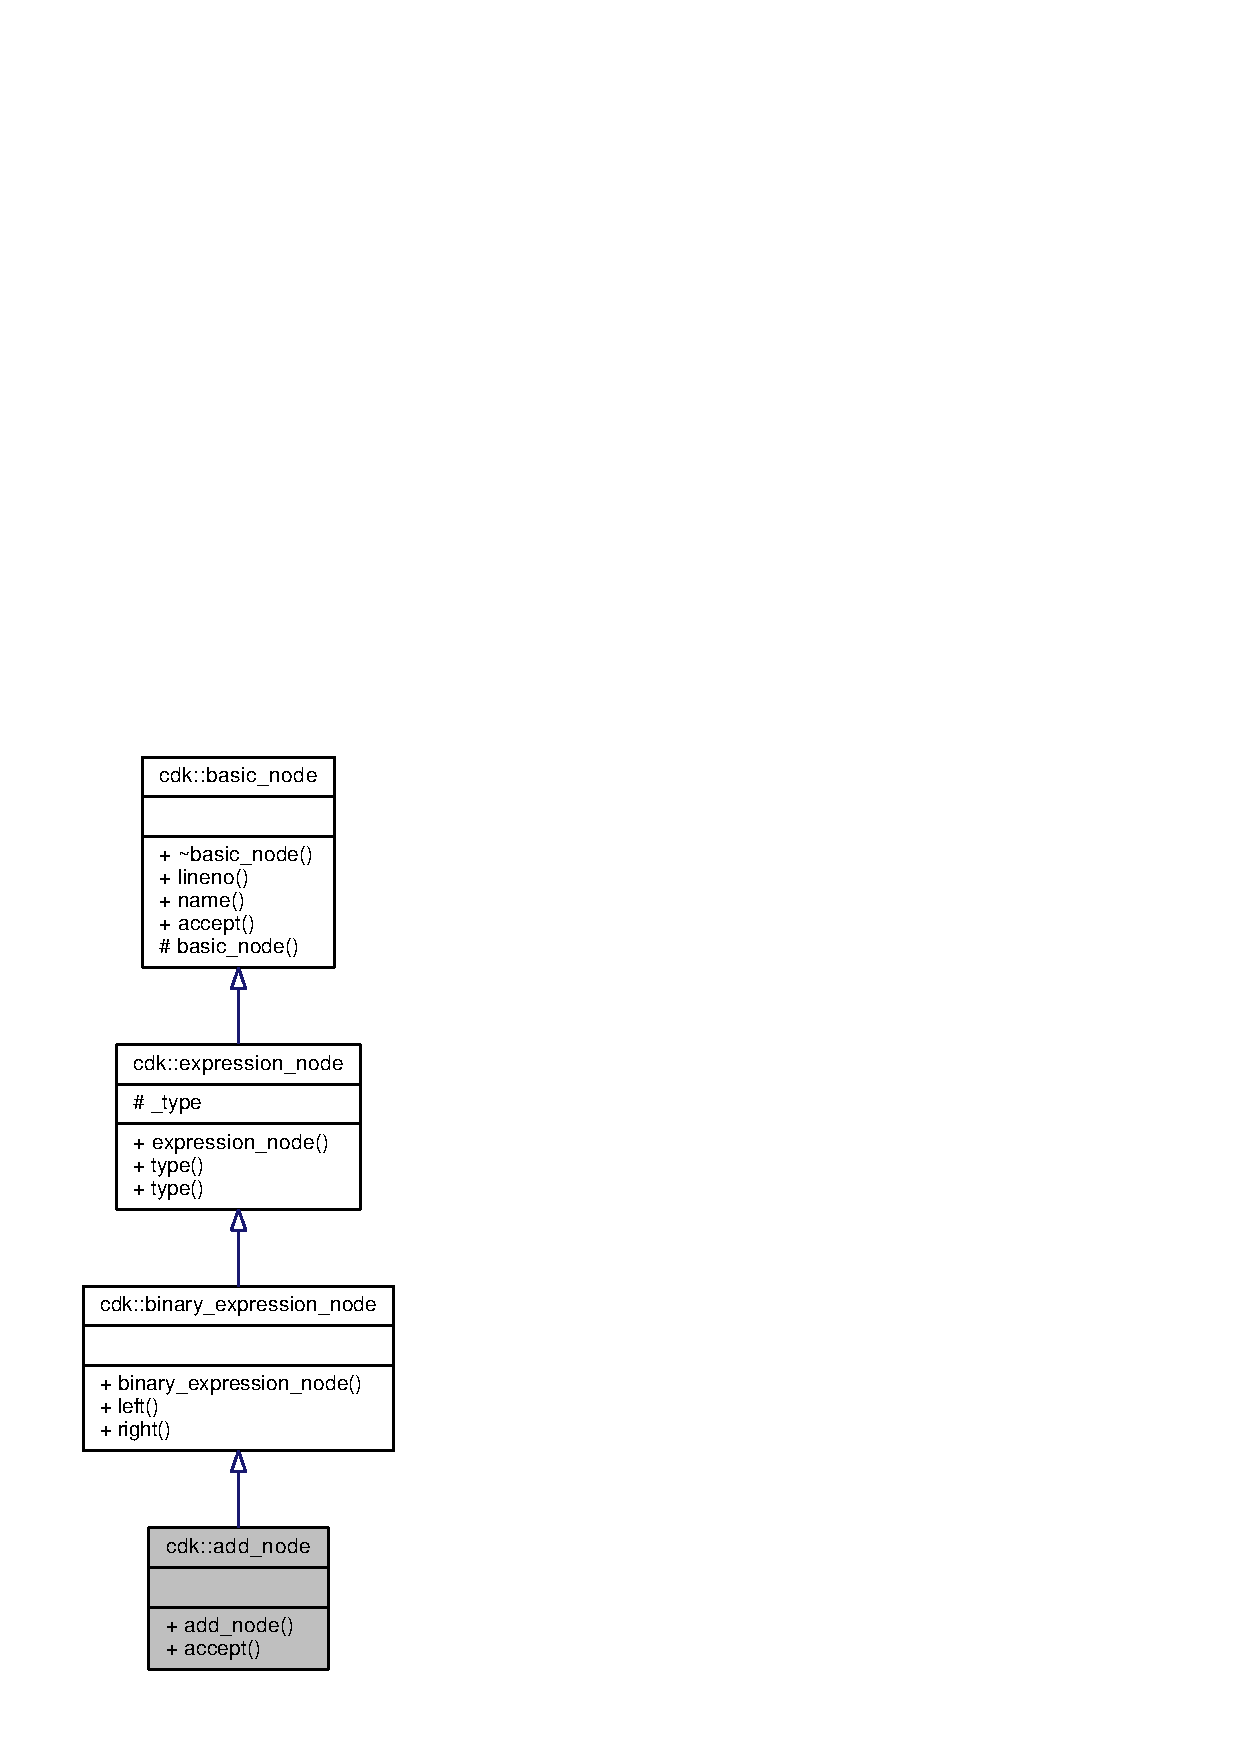
\includegraphics[width=193pt]{classcdk_1_1add__node__inherit__graph}
\end{center}
\end{figure}


Collaboration diagram for cdk\+:\+:add\+\_\+node\+:
\nopagebreak
\begin{figure}[H]
\begin{center}
\leavevmode
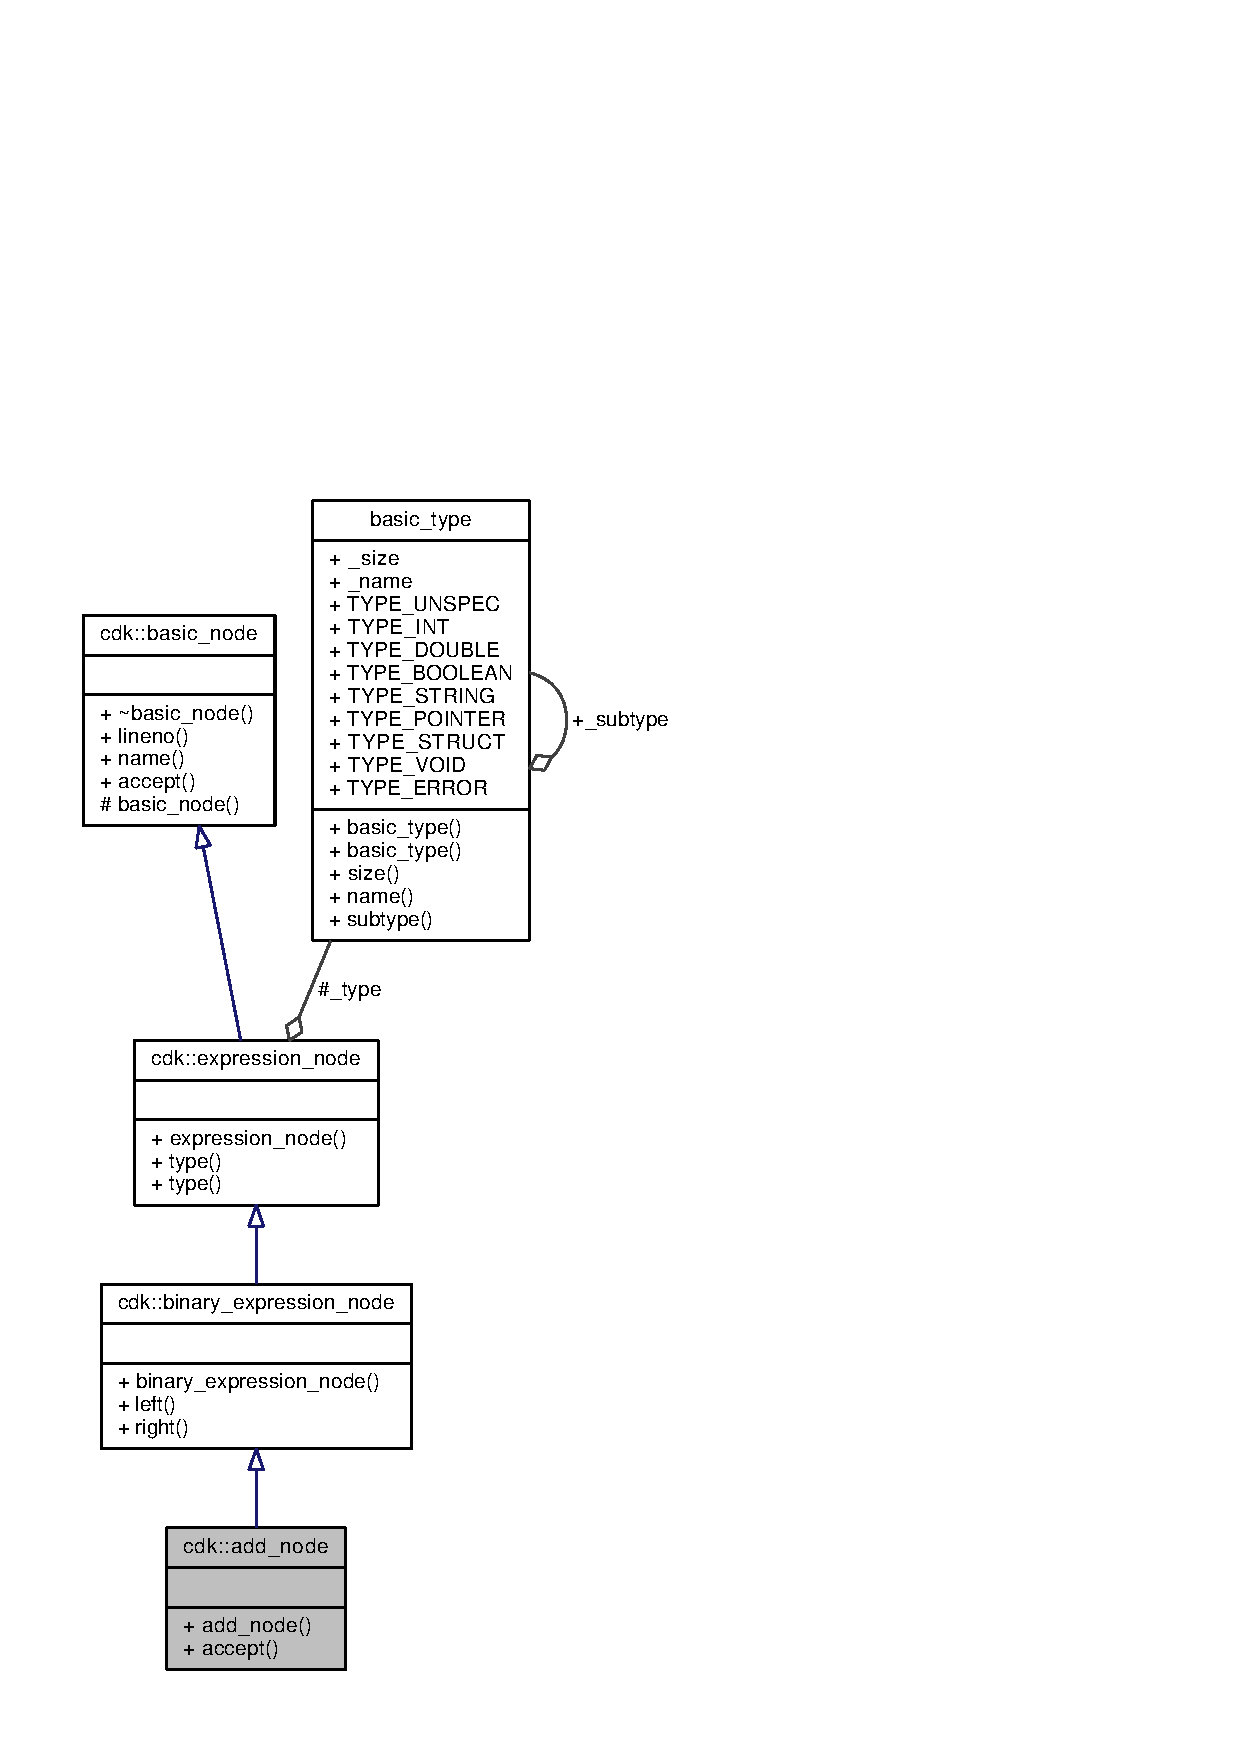
\includegraphics[height=550pt]{classcdk_1_1add__node__coll__graph}
\end{center}
\end{figure}
\subsection*{Public Member Functions}
\begin{DoxyCompactItemize}
\item 
{\bf add\+\_\+node} (int {\bf lineno}, {\bf expression\+\_\+node} $\ast$left, {\bf expression\+\_\+node} $\ast$right)
\item 
void {\bf accept} ({\bf basic\+\_\+ast\+\_\+visitor} $\ast$sp, int level)
\end{DoxyCompactItemize}
\subsection*{Additional Inherited Members}


\subsection{Detailed Description}
Class for describing the sum ('+') operator 

Definition at line 12 of file add\+\_\+node.\+h.



\subsection{Constructor \& Destructor Documentation}
\index{cdk\+::add\+\_\+node@{cdk\+::add\+\_\+node}!add\+\_\+node@{add\+\_\+node}}
\index{add\+\_\+node@{add\+\_\+node}!cdk\+::add\+\_\+node@{cdk\+::add\+\_\+node}}
\subsubsection[{add\+\_\+node}]{\setlength{\rightskip}{0pt plus 5cm}cdk\+::add\+\_\+node\+::add\+\_\+node (
\begin{DoxyParamCaption}
\item[{int}]{lineno, }
\item[{{\bf expression\+\_\+node} $\ast$}]{left, }
\item[{{\bf expression\+\_\+node} $\ast$}]{right}
\end{DoxyParamCaption}
)\hspace{0.3cm}{\ttfamily [inline]}}\label{classcdk_1_1add__node_a560eaccea3678c70d14660f91b4b349f}

\begin{DoxyParams}{Parameters}
{\em lineno} & source code line number for this node \\
\hline
{\em left} & first operand \\
\hline
{\em right} & second operand \\
\hline
\end{DoxyParams}


Definition at line 19 of file add\+\_\+node.\+h.



\subsection{Member Function Documentation}
\index{cdk\+::add\+\_\+node@{cdk\+::add\+\_\+node}!accept@{accept}}
\index{accept@{accept}!cdk\+::add\+\_\+node@{cdk\+::add\+\_\+node}}
\subsubsection[{accept}]{\setlength{\rightskip}{0pt plus 5cm}void cdk\+::add\+\_\+node\+::accept (
\begin{DoxyParamCaption}
\item[{{\bf basic\+\_\+ast\+\_\+visitor} $\ast$}]{sp, }
\item[{int}]{level}
\end{DoxyParamCaption}
)\hspace{0.3cm}{\ttfamily [inline]}, {\ttfamily [virtual]}}\label{classcdk_1_1add__node_a5a0a7fd1aacfcf589233c9b1cdda59d1}

\begin{DoxyParams}{Parameters}
{\em sp} & semantic processor visitor \\
\hline
{\em level} & syntactic tree level \\
\hline
\end{DoxyParams}


Implements {\bf cdk\+::basic\+\_\+node} \doxyref{}{p.}{classcdk_1_1basic__node_ab38adcbc95c46b809961278afae3bf05}.



Definition at line 27 of file add\+\_\+node.\+h.



The documentation for this class was generated from the following file\+:\begin{DoxyCompactItemize}
\item 
ast/add\+\_\+node.\+h\end{DoxyCompactItemize}

\section{basic\+\_\+ast\+\_\+visitor Class Reference}
\label{classbasic__ast__visitor}\index{basic\+\_\+ast\+\_\+visitor@{basic\+\_\+ast\+\_\+visitor}}


{\ttfamily \#include $<$basic\+\_\+ast\+\_\+visitor.\+h$>$}



Collaboration diagram for basic\+\_\+ast\+\_\+visitor\+:
\nopagebreak
\begin{figure}[H]
\begin{center}
\leavevmode
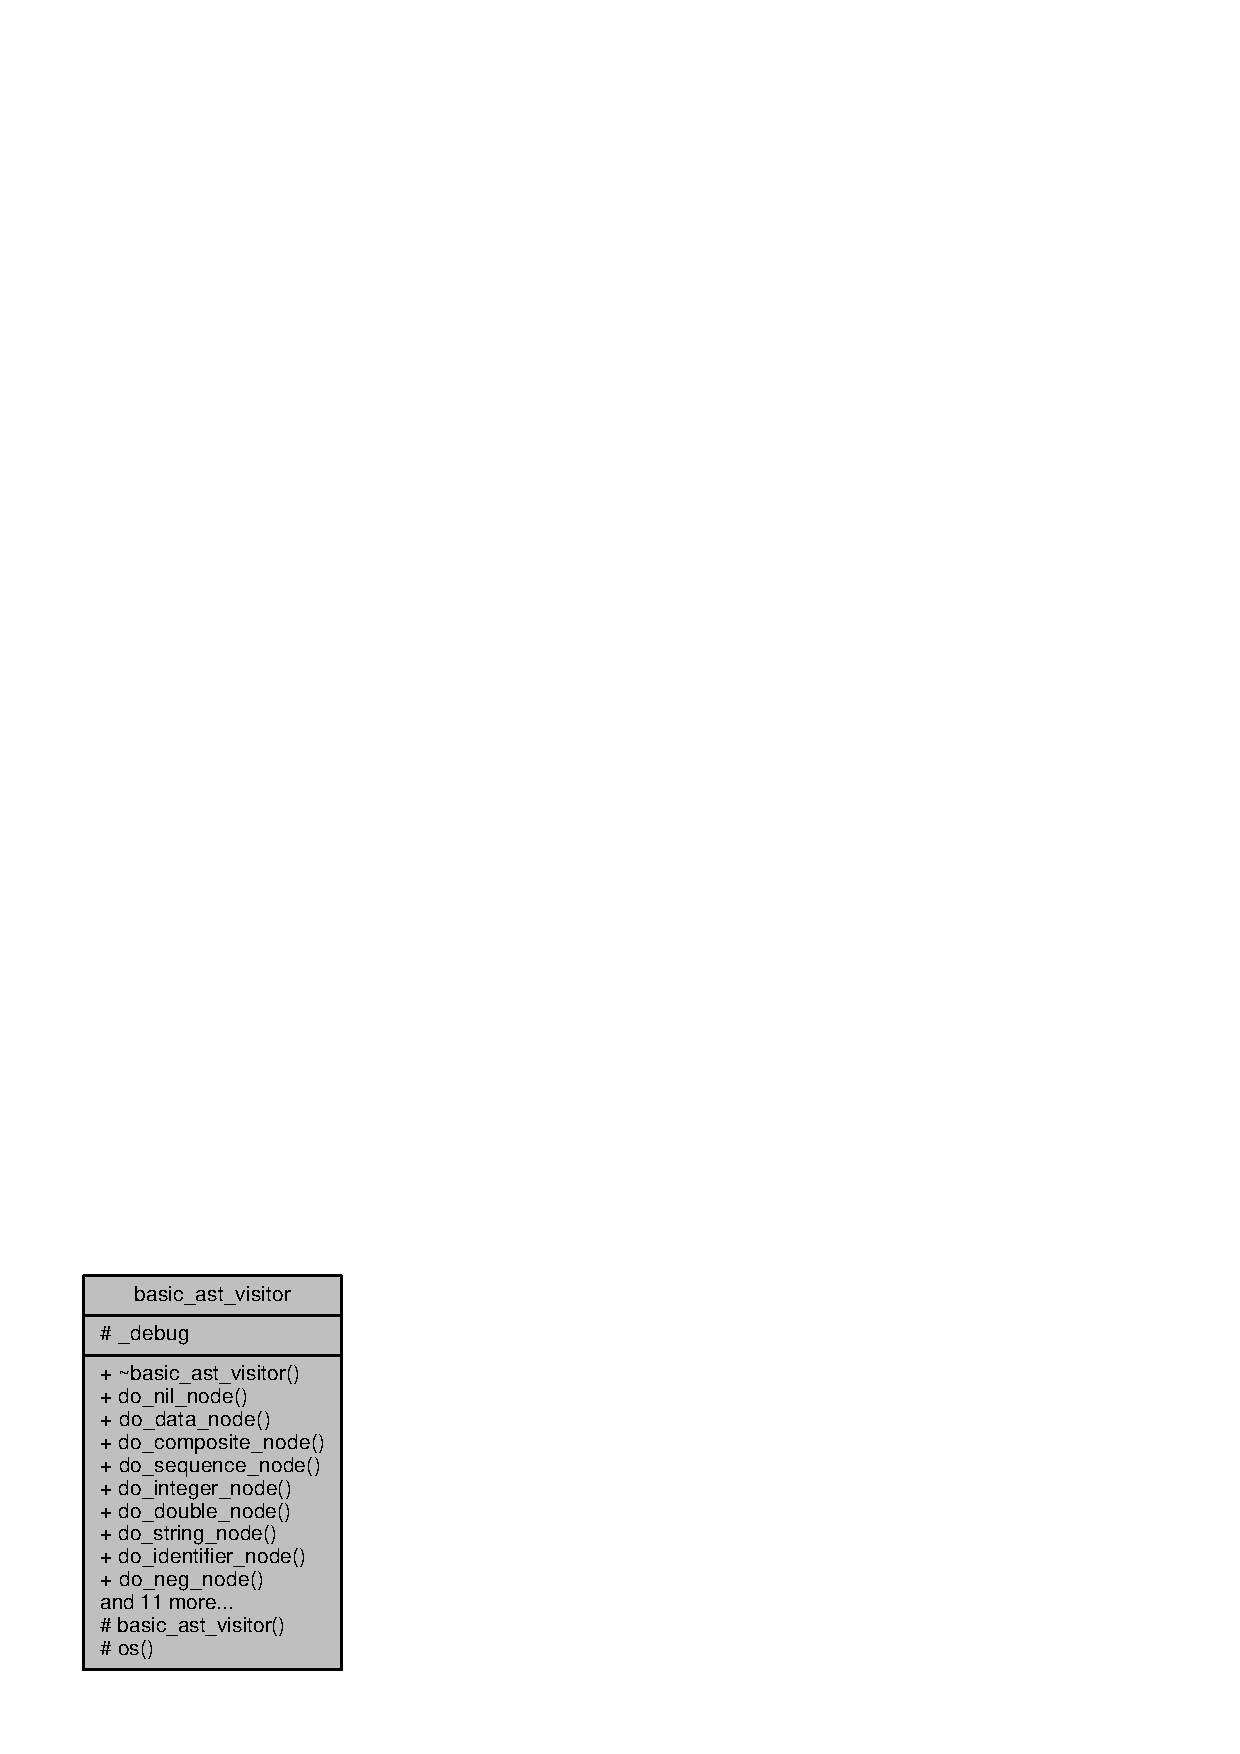
\includegraphics[width=168pt]{classbasic__ast__visitor__coll__graph}
\end{center}
\end{figure}
\subsection*{Public Member Functions}
\begin{DoxyCompactItemize}
\item 
virtual {\bf $\sim$basic\+\_\+ast\+\_\+visitor} ()
\item 
virtual void {\bfseries do\+\_\+nil\+\_\+node} ({\bf cdk\+::nil\+\_\+node} $\ast$const node, int lvl)=0\label{classbasic__ast__visitor_a02f54aebc971eb949ef263b972c1d5c9}

\item 
virtual void {\bfseries do\+\_\+data\+\_\+node} ({\bf cdk\+::data\+\_\+node} $\ast$const node, int lvl)=0\label{classbasic__ast__visitor_a92a91d350c0447876448dc89adb872d6}

\item 
virtual void {\bfseries do\+\_\+composite\+\_\+node} ({\bf cdk\+::composite\+\_\+node} $\ast$const node, int lvl)=0\label{classbasic__ast__visitor_a0b5b9548265a03019141b63c7f5934b4}

\item 
virtual void {\bfseries do\+\_\+sequence\+\_\+node} ({\bf cdk\+::sequence\+\_\+node} $\ast$const node, int lvl)=0\label{classbasic__ast__visitor_adfbe26d736fab220458165a60888e563}

\item 
virtual void {\bfseries do\+\_\+integer\+\_\+node} ({\bf cdk\+::integer\+\_\+node} $\ast$const node, int lvl)=0\label{classbasic__ast__visitor_a16cb8f6c1790a95f3e65019272645d0d}

\item 
virtual void {\bfseries do\+\_\+double\+\_\+node} ({\bf cdk\+::double\+\_\+node} $\ast$const node, int lvl)=0\label{classbasic__ast__visitor_ad44ac45e5172600955897fc6669bf14e}

\item 
virtual void {\bfseries do\+\_\+string\+\_\+node} ({\bf cdk\+::string\+\_\+node} $\ast$const node, int lvl)=0\label{classbasic__ast__visitor_a3f030ce97bbd3f136d7208dd8820d848}

\item 
virtual void {\bfseries do\+\_\+identifier\+\_\+node} ({\bf cdk\+::identifier\+\_\+node} $\ast$const node, int lvl)=0\label{classbasic__ast__visitor_a1e8c56656489408c46def651164c0506}

\item 
virtual void {\bfseries do\+\_\+neg\+\_\+node} ({\bf cdk\+::neg\+\_\+node} $\ast$const node, int lvl)=0\label{classbasic__ast__visitor_a0f8aab79e4982b9165c4f2073d0a0791}

\item 
virtual void {\bfseries do\+\_\+add\+\_\+node} ({\bf cdk\+::add\+\_\+node} $\ast$const node, int lvl)=0\label{classbasic__ast__visitor_acaf61e947882fe332740272a88d40dff}

\item 
virtual void {\bfseries do\+\_\+sub\+\_\+node} ({\bf cdk\+::sub\+\_\+node} $\ast$const node, int lvl)=0\label{classbasic__ast__visitor_ac22ba53376b0df09fcbce78030568d1b}

\item 
virtual void {\bfseries do\+\_\+mul\+\_\+node} ({\bf cdk\+::mul\+\_\+node} $\ast$const node, int lvl)=0\label{classbasic__ast__visitor_a7806c518f8fb3f9349b3b56a0ec266be}

\item 
virtual void {\bfseries do\+\_\+div\+\_\+node} ({\bf cdk\+::div\+\_\+node} $\ast$const node, int lvl)=0\label{classbasic__ast__visitor_abea4863f6219fb67e1841620d08a882d}

\item 
virtual void {\bfseries do\+\_\+mod\+\_\+node} ({\bf cdk\+::mod\+\_\+node} $\ast$const node, int lvl)=0\label{classbasic__ast__visitor_ad7ad0bac59f46e8a8eae65506973f3bb}

\item 
virtual void {\bfseries do\+\_\+lt\+\_\+node} ({\bf cdk\+::lt\+\_\+node} $\ast$const node, int lvl)=0\label{classbasic__ast__visitor_a1167e428d37a80936ebb6c99638c70ca}

\item 
virtual void {\bfseries do\+\_\+le\+\_\+node} ({\bf cdk\+::le\+\_\+node} $\ast$const node, int lvl)=0\label{classbasic__ast__visitor_a51d63c3b08b977f75ecef38dcd10f919}

\item 
virtual void {\bfseries do\+\_\+ge\+\_\+node} ({\bf cdk\+::ge\+\_\+node} $\ast$const node, int lvl)=0\label{classbasic__ast__visitor_a50cb4319b9ba03376fe567a92a0fb1ab}

\item 
virtual void {\bfseries do\+\_\+gt\+\_\+node} ({\bf cdk\+::gt\+\_\+node} $\ast$const node, int lvl)=0\label{classbasic__ast__visitor_a35d5c3dd16c3eec5797d67324608fd68}

\item 
virtual void {\bfseries do\+\_\+ne\+\_\+node} ({\bf cdk\+::ne\+\_\+node} $\ast$const node, int lvl)=0\label{classbasic__ast__visitor_adef6c9af687ca4c1a84d4e6b2f89f43c}

\item 
virtual void {\bfseries do\+\_\+eq\+\_\+node} ({\bf cdk\+::eq\+\_\+node} $\ast$const node, int lvl)=0\label{classbasic__ast__visitor_a28c9f578ae839fe555cd92615e8c2acb}

\end{DoxyCompactItemize}
\subsection*{Protected Member Functions}
\begin{DoxyCompactItemize}
\item 
{\bf basic\+\_\+ast\+\_\+visitor} (std\+::ostream \&{\bf os}=std\+::cout, bool debug=false)
\item 
std\+::ostream \& {\bf os} ()
\end{DoxyCompactItemize}
\subsection*{Protected Attributes}
\begin{DoxyCompactItemize}
\item 
bool {\bf \+\_\+debug}\label{classbasic__ast__visitor_a00d9f815e553a3313b33a952e03702f4}

\begin{DoxyCompactList}\small\item\em Debug flag. \end{DoxyCompactList}\end{DoxyCompactItemize}


\subsection{Detailed Description}
This class is only for compiling the package\+: it will not be installed. Specific compilers are supposed to define their own, with the S\+A\+M\+E N\+A\+M\+E, but defining A\+L\+L processing functions corresponding to their specific problem. 

Definition at line 41 of file basic\+\_\+ast\+\_\+visitor.\+h.



\subsection{Constructor \& Destructor Documentation}
\index{basic\+\_\+ast\+\_\+visitor@{basic\+\_\+ast\+\_\+visitor}!basic\+\_\+ast\+\_\+visitor@{basic\+\_\+ast\+\_\+visitor}}
\index{basic\+\_\+ast\+\_\+visitor@{basic\+\_\+ast\+\_\+visitor}!basic\+\_\+ast\+\_\+visitor@{basic\+\_\+ast\+\_\+visitor}}
\subsubsection[{basic\+\_\+ast\+\_\+visitor}]{\setlength{\rightskip}{0pt plus 5cm}basic\+\_\+ast\+\_\+visitor\+::basic\+\_\+ast\+\_\+visitor (
\begin{DoxyParamCaption}
\item[{std\+::ostream \&}]{os = {\ttfamily std\+:\+:cout}, }
\item[{bool}]{debug = {\ttfamily false}}
\end{DoxyParamCaption}
)\hspace{0.3cm}{\ttfamily [protected]}}\label{classbasic__ast__visitor_a194d2f7cced321e384b68782d8e33a47}
Initialization of a semantic processor.


\begin{DoxyParams}{Parameters}
{\em os} & is the output stream to be used by the semantic processor. \\
\hline
\end{DoxyParams}
\index{basic\+\_\+ast\+\_\+visitor@{basic\+\_\+ast\+\_\+visitor}!````~basic\+\_\+ast\+\_\+visitor@{$\sim$basic\+\_\+ast\+\_\+visitor}}
\index{````~basic\+\_\+ast\+\_\+visitor@{$\sim$basic\+\_\+ast\+\_\+visitor}!basic\+\_\+ast\+\_\+visitor@{basic\+\_\+ast\+\_\+visitor}}
\subsubsection[{$\sim$basic\+\_\+ast\+\_\+visitor}]{\setlength{\rightskip}{0pt plus 5cm}virtual basic\+\_\+ast\+\_\+visitor\+::$\sim$basic\+\_\+ast\+\_\+visitor (
\begin{DoxyParamCaption}
{}
\end{DoxyParamCaption}
)\hspace{0.3cm}{\ttfamily [virtual]}}\label{classbasic__ast__visitor_a110508f9dd86fc1472ffee3d2b3bd0f5}
How to destroy a semantic processor. 

\subsection{Member Function Documentation}
\index{basic\+\_\+ast\+\_\+visitor@{basic\+\_\+ast\+\_\+visitor}!os@{os}}
\index{os@{os}!basic\+\_\+ast\+\_\+visitor@{basic\+\_\+ast\+\_\+visitor}}
\subsubsection[{os}]{\setlength{\rightskip}{0pt plus 5cm}std\+::ostream\& basic\+\_\+ast\+\_\+visitor\+::os (
\begin{DoxyParamCaption}
{}
\end{DoxyParamCaption}
)\hspace{0.3cm}{\ttfamily [inline]}, {\ttfamily [protected]}}\label{classbasic__ast__visitor_ab81ab147fe687470c3e8f9ebfd2ca6f9}
Return the current output stream. \begin{DoxyReturn}{Returns}
an output stream. 
\end{DoxyReturn}


Definition at line 62 of file basic\+\_\+ast\+\_\+visitor.\+h.



The documentation for this class was generated from the following file\+:\begin{DoxyCompactItemize}
\item 
basic\+\_\+ast\+\_\+visitor.\+h\end{DoxyCompactItemize}

\section{cdk\+:\+:basic\+\_\+factory Class Reference}
\label{classcdk_1_1basic__factory}\index{cdk\+::basic\+\_\+factory@{cdk\+::basic\+\_\+factory}}


{\ttfamily \#include $<$basic\+\_\+factory.\+h$>$}



Inheritance diagram for cdk\+:\+:basic\+\_\+factory\+:
\nopagebreak
\begin{figure}[H]
\begin{center}
\leavevmode
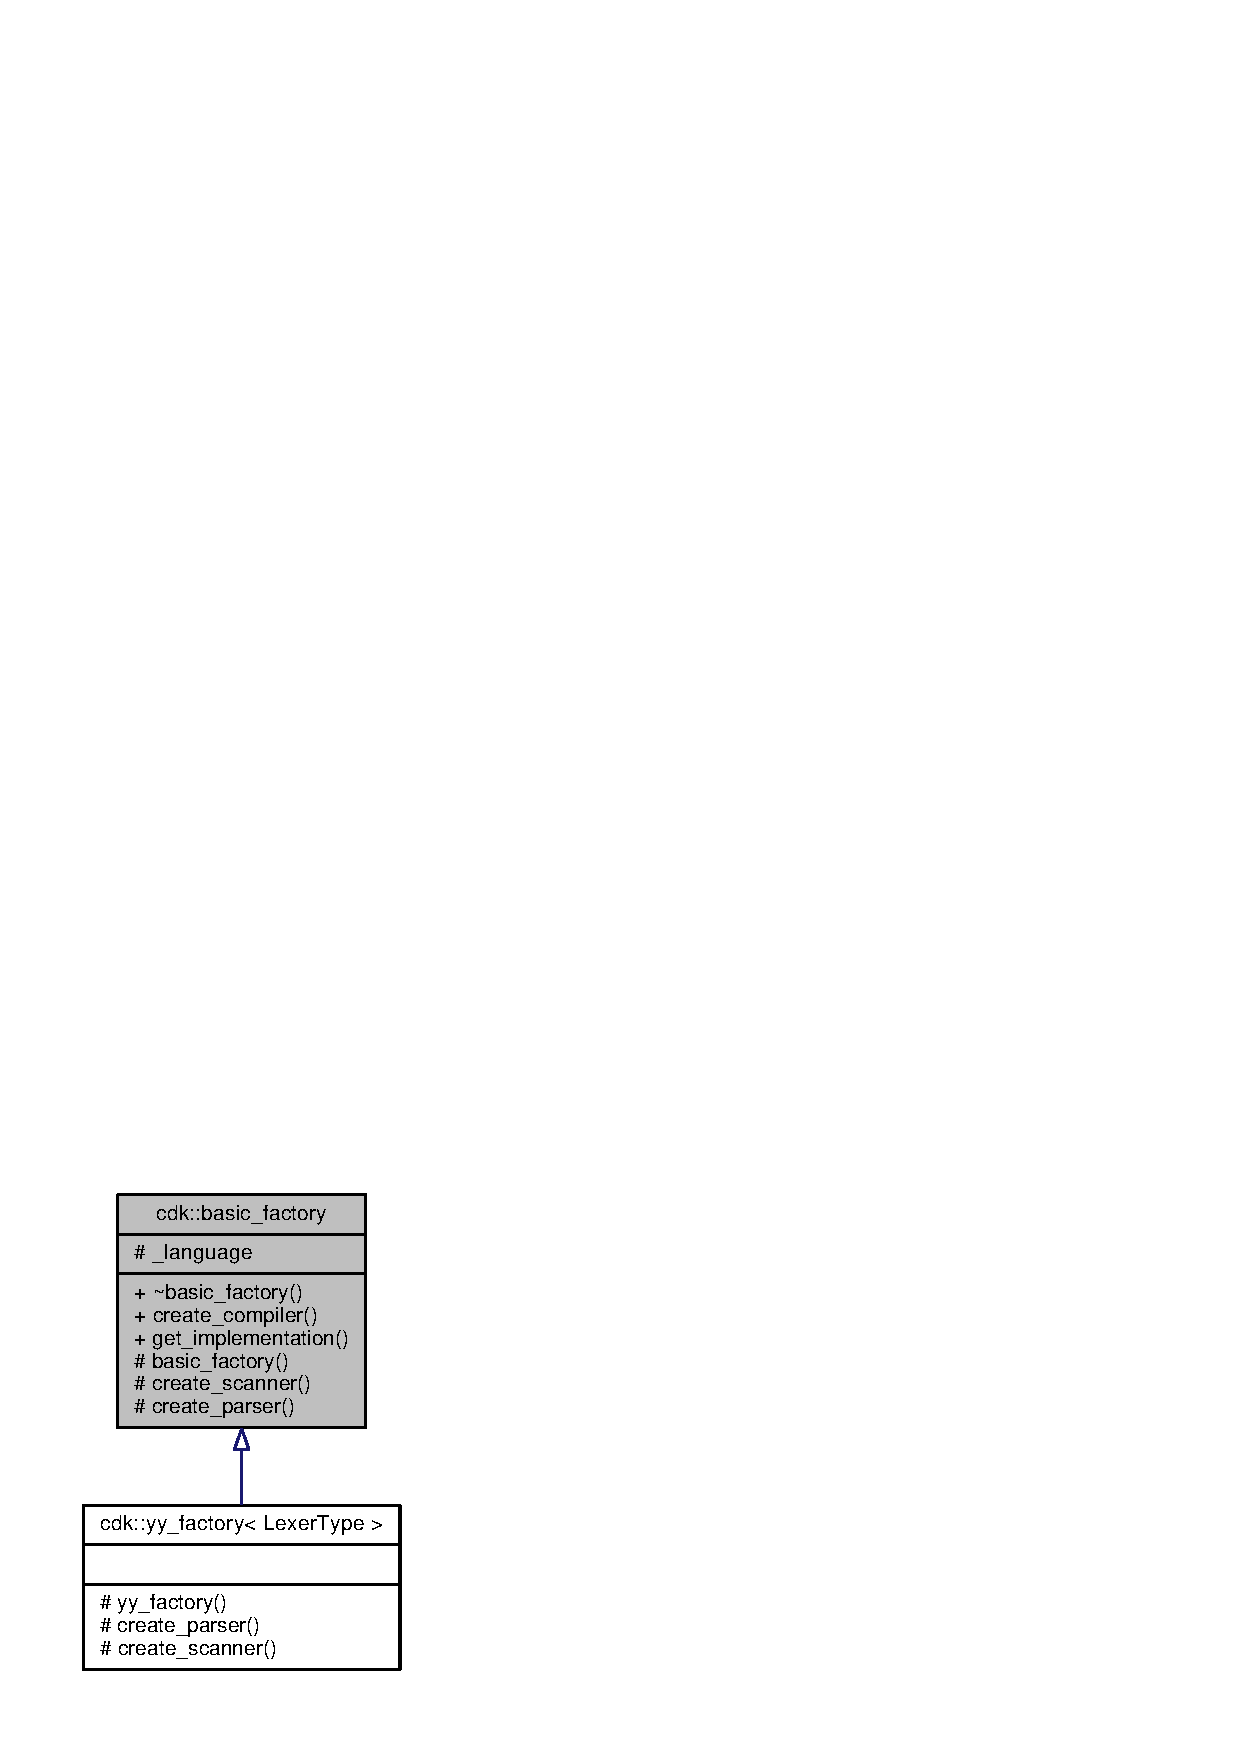
\includegraphics[width=196pt]{classcdk_1_1basic__factory__inherit__graph}
\end{center}
\end{figure}


Collaboration diagram for cdk\+:\+:basic\+\_\+factory\+:
\nopagebreak
\begin{figure}[H]
\begin{center}
\leavevmode
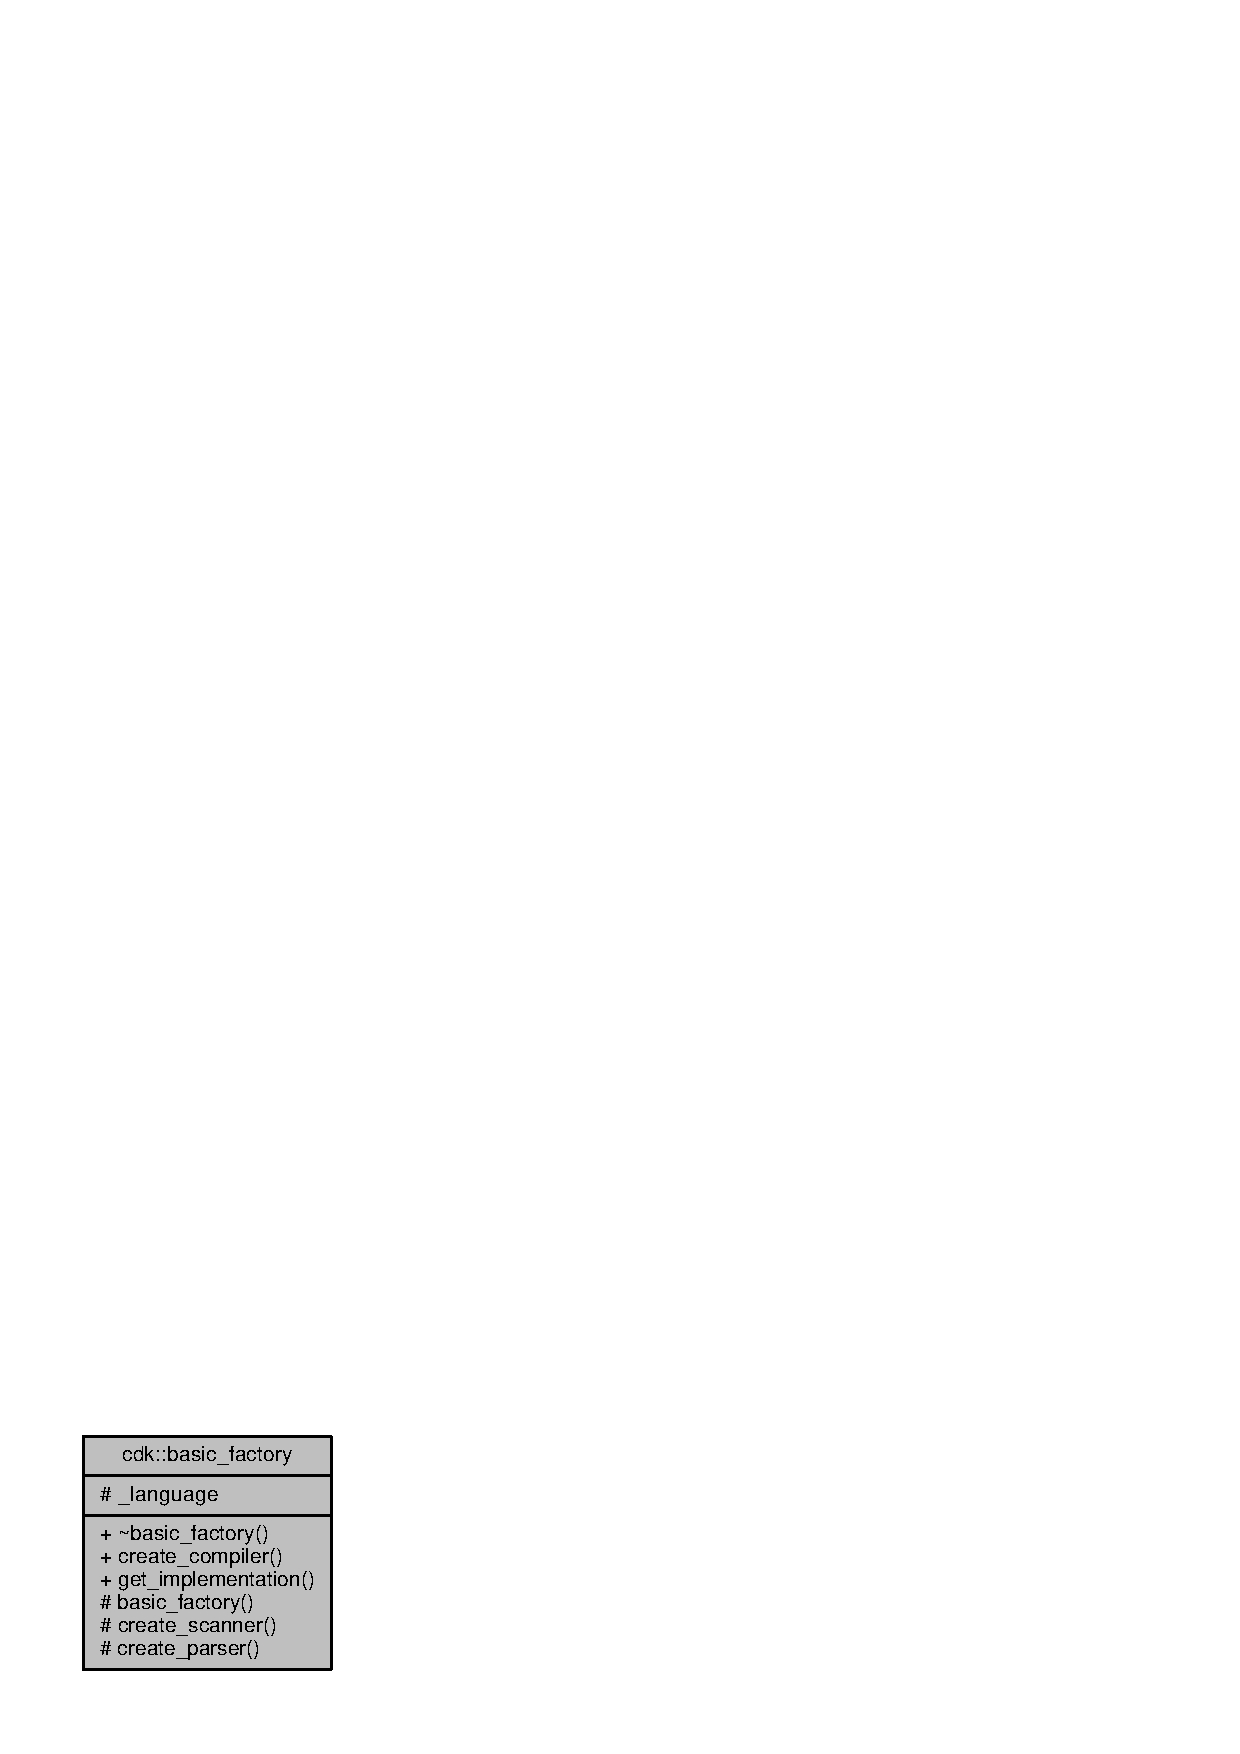
\includegraphics[width=163pt]{classcdk_1_1basic__factory__coll__graph}
\end{center}
\end{figure}
\subsection*{Public Member Functions}
\begin{DoxyCompactItemize}
\item 
virtual {\bf $\sim$basic\+\_\+factory} ()
\item 
virtual std\+::shared\+\_\+ptr$<$ {\bf compiler} $>$ {\bf create\+\_\+compiler} ()
\end{DoxyCompactItemize}
\subsection*{Static Public Member Functions}
\begin{DoxyCompactItemize}
\item 
static {\bf basic\+\_\+factory} $\ast$ {\bfseries get\+\_\+implementation} (const std\+::string \&language)\label{classcdk_1_1basic__factory_a535fded0c301dc7d002f17fe631d5fa9}

\end{DoxyCompactItemize}
\subsection*{Protected Member Functions}
\begin{DoxyCompactItemize}
\item 
{\bfseries basic\+\_\+factory} (const std\+::string \&language)\label{classcdk_1_1basic__factory_ad6019ad813cd6a082284cd4265d2ea5a}

\item 
virtual std\+::shared\+\_\+ptr\\*
$<$ {\bf basic\+\_\+scanner} $>$ {\bf create\+\_\+scanner} ()=0
\item 
virtual std\+::shared\+\_\+ptr\\*
$<$ {\bf basic\+\_\+parser} $>$ {\bf create\+\_\+parser} ()=0
\end{DoxyCompactItemize}
\subsection*{Protected Attributes}
\begin{DoxyCompactItemize}
\item 
const std\+::string {\bfseries \+\_\+language} = \char`\"{}\char`\"{}\label{classcdk_1_1basic__factory_a8c4a1162265812837a9a001973cc9a3a}

\end{DoxyCompactItemize}


\subsection{Detailed Description}
This is the main factory abstract class\+: it provides methods for creating the lexical analyser and the compiler itself. Instances of concrete subclasses will be created by the \char`\"{}main\char`\"{} function to provide instances of the scanner and compiler objects for a concrete language.
\begin{DoxyItemize}
\item keys are language names
\item values are compiler factories 
\end{DoxyItemize}

Definition at line 25 of file basic\+\_\+factory.\+h.



\subsection{Constructor \& Destructor Documentation}
\index{cdk\+::basic\+\_\+factory@{cdk\+::basic\+\_\+factory}!````~basic\+\_\+factory@{$\sim$basic\+\_\+factory}}
\index{````~basic\+\_\+factory@{$\sim$basic\+\_\+factory}!cdk\+::basic\+\_\+factory@{cdk\+::basic\+\_\+factory}}
\subsubsection[{$\sim$basic\+\_\+factory}]{\setlength{\rightskip}{0pt plus 5cm}virtual cdk\+::basic\+\_\+factory\+::$\sim$basic\+\_\+factory (
\begin{DoxyParamCaption}
{}
\end{DoxyParamCaption}
)\hspace{0.3cm}{\ttfamily [inline]}, {\ttfamily [virtual]}}\label{classcdk_1_1basic__factory_a9cb78539bfef6fef3429337c42b78554}
The superclass destructor does not do anything. Probably, it would be a good idea to clean up the factories map. 

Definition at line 53 of file basic\+\_\+factory.\+h.



\subsection{Member Function Documentation}
\index{cdk\+::basic\+\_\+factory@{cdk\+::basic\+\_\+factory}!create\+\_\+compiler@{create\+\_\+compiler}}
\index{create\+\_\+compiler@{create\+\_\+compiler}!cdk\+::basic\+\_\+factory@{cdk\+::basic\+\_\+factory}}
\subsubsection[{create\+\_\+compiler}]{\setlength{\rightskip}{0pt plus 5cm}virtual std\+::shared\+\_\+ptr$<${\bf compiler}$>$ cdk\+::basic\+\_\+factory\+::create\+\_\+compiler (
\begin{DoxyParamCaption}
{}
\end{DoxyParamCaption}
)\hspace{0.3cm}{\ttfamily [inline]}, {\ttfamily [virtual]}}\label{classcdk_1_1basic__factory_a883cf0f3e52b5a53b316914c74535de7}
Create a compiler object for a given language. 
\begin{DoxyParams}{Parameters}
{\em name} & name of the language handled by the compiler \\
\hline
\end{DoxyParams}
\begin{DoxyReturn}{Returns}
compiler object pointer 
\end{DoxyReturn}


Definition at line 79 of file basic\+\_\+factory.\+h.



References create\+\_\+parser(), and create\+\_\+scanner().



Here is the call graph for this function\+:
\nopagebreak
\begin{figure}[H]
\begin{center}
\leavevmode
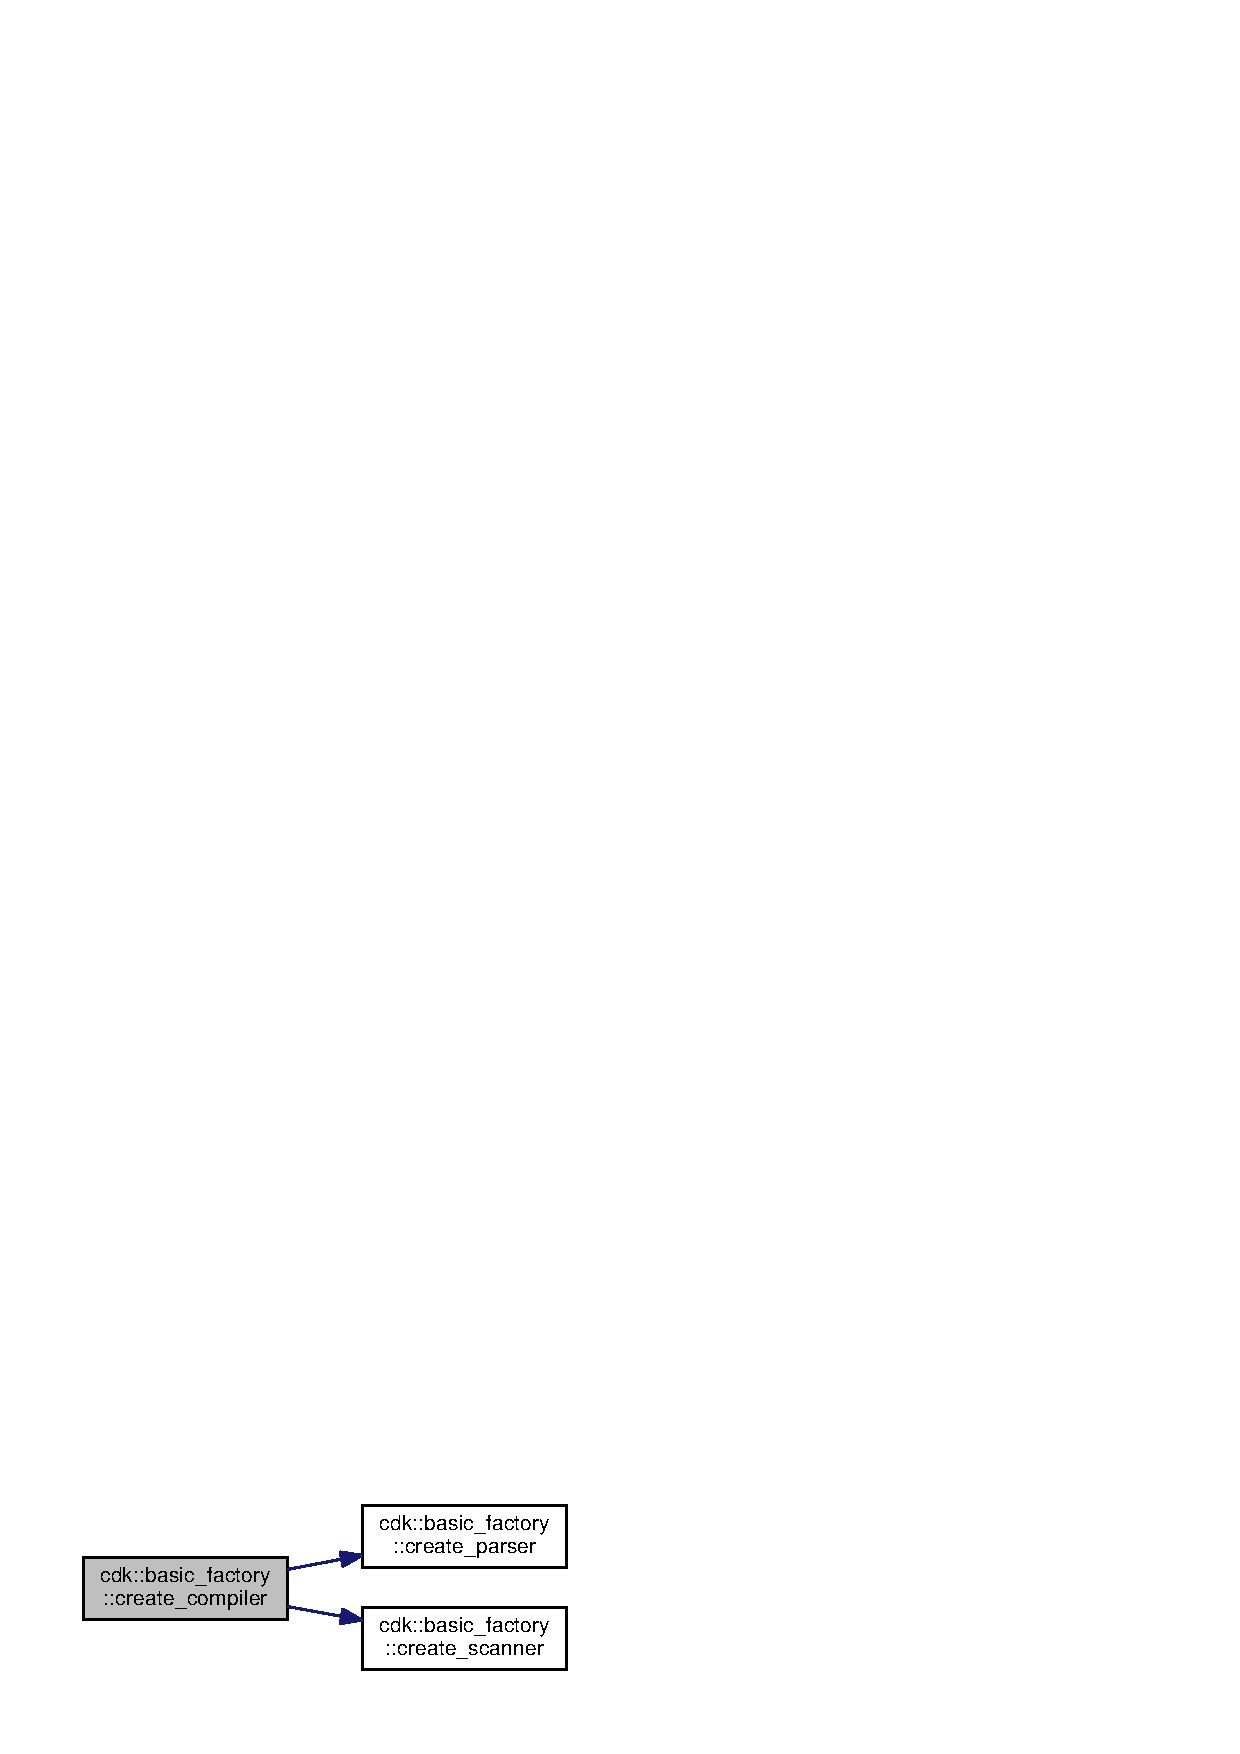
\includegraphics[width=276pt]{classcdk_1_1basic__factory_a883cf0f3e52b5a53b316914c74535de7_cgraph}
\end{center}
\end{figure}


\index{cdk\+::basic\+\_\+factory@{cdk\+::basic\+\_\+factory}!create\+\_\+parser@{create\+\_\+parser}}
\index{create\+\_\+parser@{create\+\_\+parser}!cdk\+::basic\+\_\+factory@{cdk\+::basic\+\_\+factory}}
\subsubsection[{create\+\_\+parser}]{\setlength{\rightskip}{0pt plus 5cm}virtual std\+::shared\+\_\+ptr$<${\bf basic\+\_\+parser}$>$ cdk\+::basic\+\_\+factory\+::create\+\_\+parser (
\begin{DoxyParamCaption}
{}
\end{DoxyParamCaption}
)\hspace{0.3cm}{\ttfamily [protected]}, {\ttfamily [pure virtual]}}\label{classcdk_1_1basic__factory_afc8f88801455bf131cc4039271e6b741}
Create a parser object for a given language. 
\begin{DoxyParams}{Parameters}
{\em name} & name of the input file (for debug only) \\
\hline
\end{DoxyParams}
\begin{DoxyReturn}{Returns}
parser object pointer 
\end{DoxyReturn}
\begin{DoxySeeAlso}{See also}
create\+Compiler 
\end{DoxySeeAlso}


Implemented in {\bf cdk\+::yy\+\_\+factory$<$ Lexer\+Type $>$} \doxyref{}{p.}{classcdk_1_1yy__factory_a9a051ba49001a7dbb9822b64c45135e9}.



Referenced by create\+\_\+compiler().

\index{cdk\+::basic\+\_\+factory@{cdk\+::basic\+\_\+factory}!create\+\_\+scanner@{create\+\_\+scanner}}
\index{create\+\_\+scanner@{create\+\_\+scanner}!cdk\+::basic\+\_\+factory@{cdk\+::basic\+\_\+factory}}
\subsubsection[{create\+\_\+scanner}]{\setlength{\rightskip}{0pt plus 5cm}virtual std\+::shared\+\_\+ptr$<${\bf basic\+\_\+scanner}$>$ cdk\+::basic\+\_\+factory\+::create\+\_\+scanner (
\begin{DoxyParamCaption}
{}
\end{DoxyParamCaption}
)\hspace{0.3cm}{\ttfamily [protected]}, {\ttfamily [pure virtual]}}\label{classcdk_1_1basic__factory_a25f3a81be472baccf2ab5ffb2f363608}
Create a scanner object for a given language. 
\begin{DoxyParams}{Parameters}
{\em name} & name of the input file (for debug only) \\
\hline
\end{DoxyParams}
\begin{DoxyReturn}{Returns}
scanner object pointer 
\end{DoxyReturn}
\begin{DoxySeeAlso}{See also}
create\+Compiler 
\end{DoxySeeAlso}


Implemented in {\bf cdk\+::yy\+\_\+factory$<$ Lexer\+Type $>$} \doxyref{}{p.}{classcdk_1_1yy__factory_a6132d875a397d6207727b070ed4155de}.



Referenced by create\+\_\+compiler().



The documentation for this class was generated from the following file\+:\begin{DoxyCompactItemize}
\item 
basic\+\_\+factory.\+h\end{DoxyCompactItemize}

\section{cdk\+:\+:basic\+\_\+node Class Reference}
\label{classcdk_1_1basic__node}\index{cdk\+::basic\+\_\+node@{cdk\+::basic\+\_\+node}}


{\ttfamily \#include $<$basic\+\_\+node.\+h$>$}



Inheritance diagram for cdk\+:\+:basic\+\_\+node\+:
\nopagebreak
\begin{figure}[H]
\begin{center}
\leavevmode
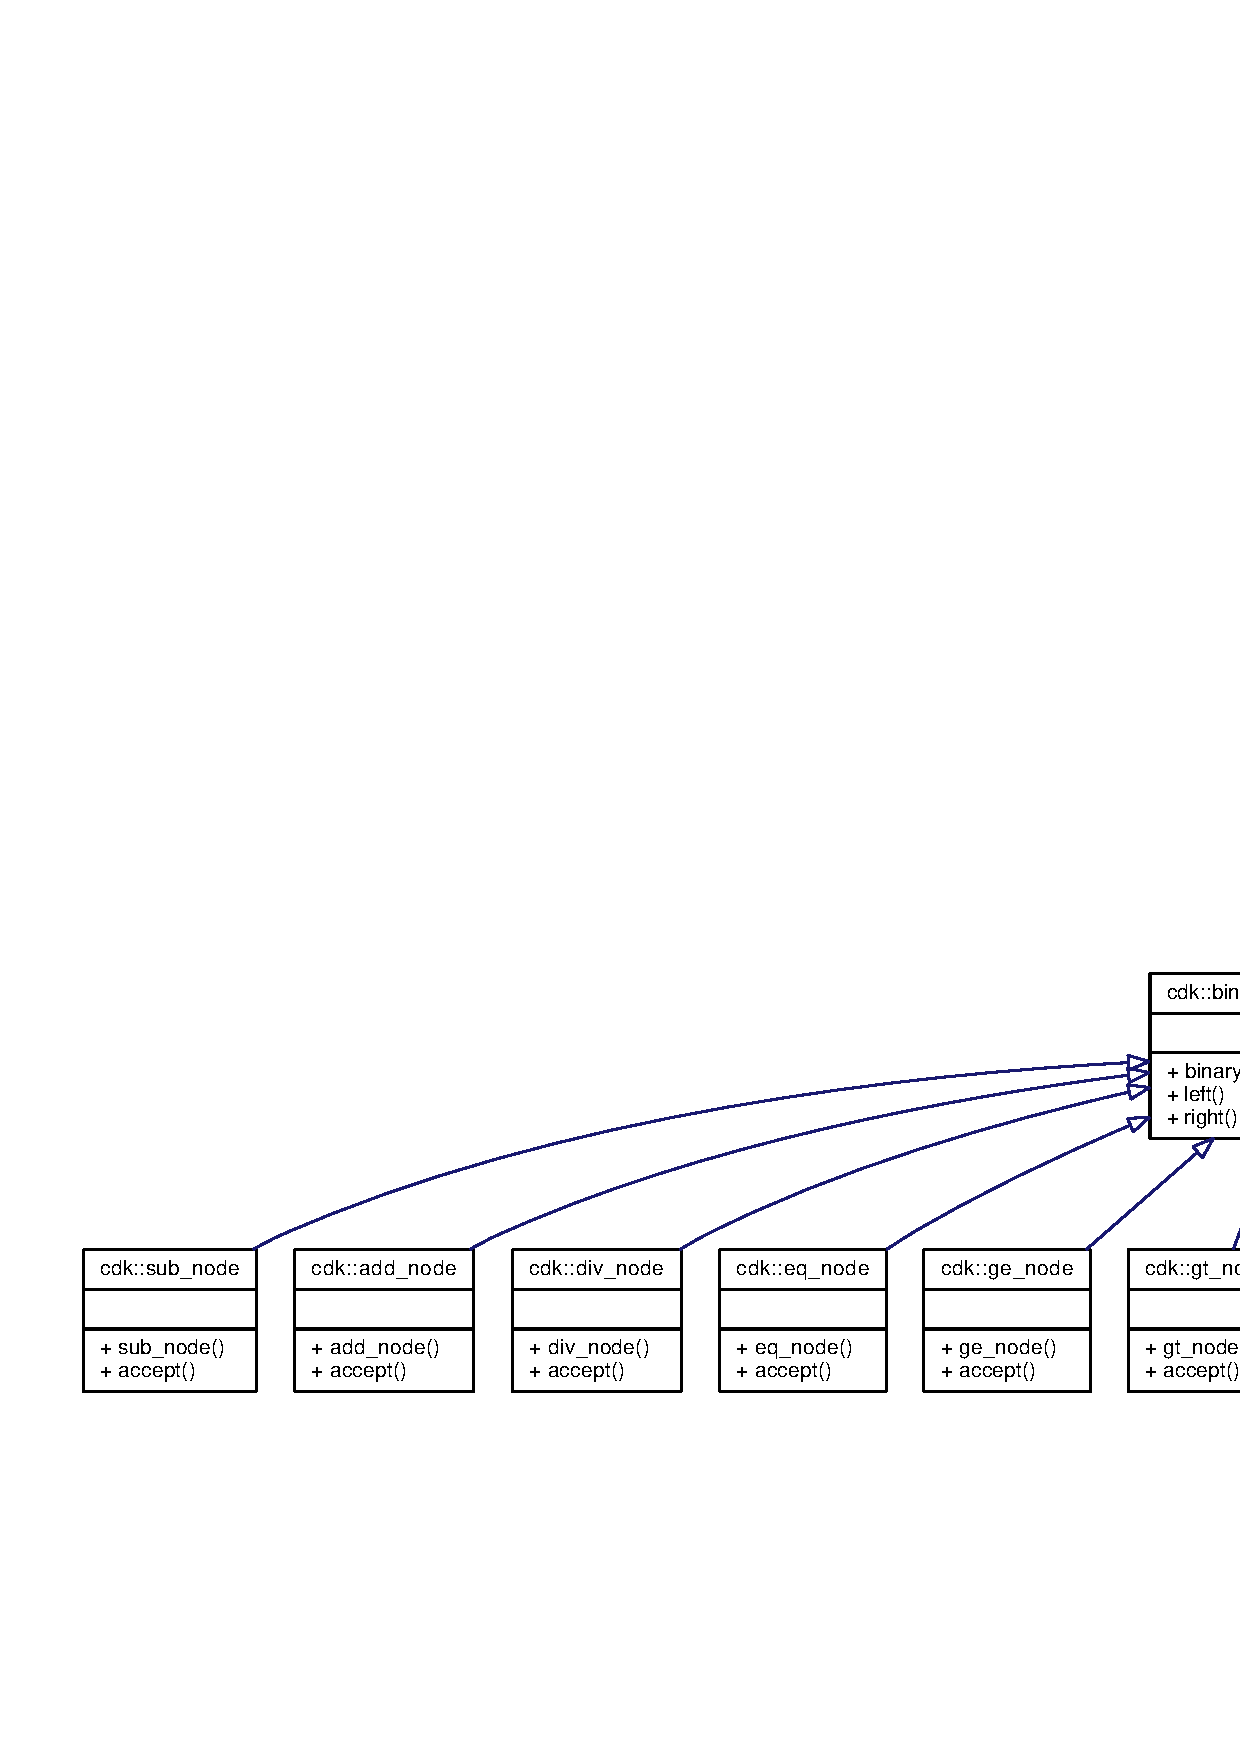
\includegraphics[width=350pt]{classcdk_1_1basic__node__inherit__graph}
\end{center}
\end{figure}


Collaboration diagram for cdk\+:\+:basic\+\_\+node\+:
\nopagebreak
\begin{figure}[H]
\begin{center}
\leavevmode
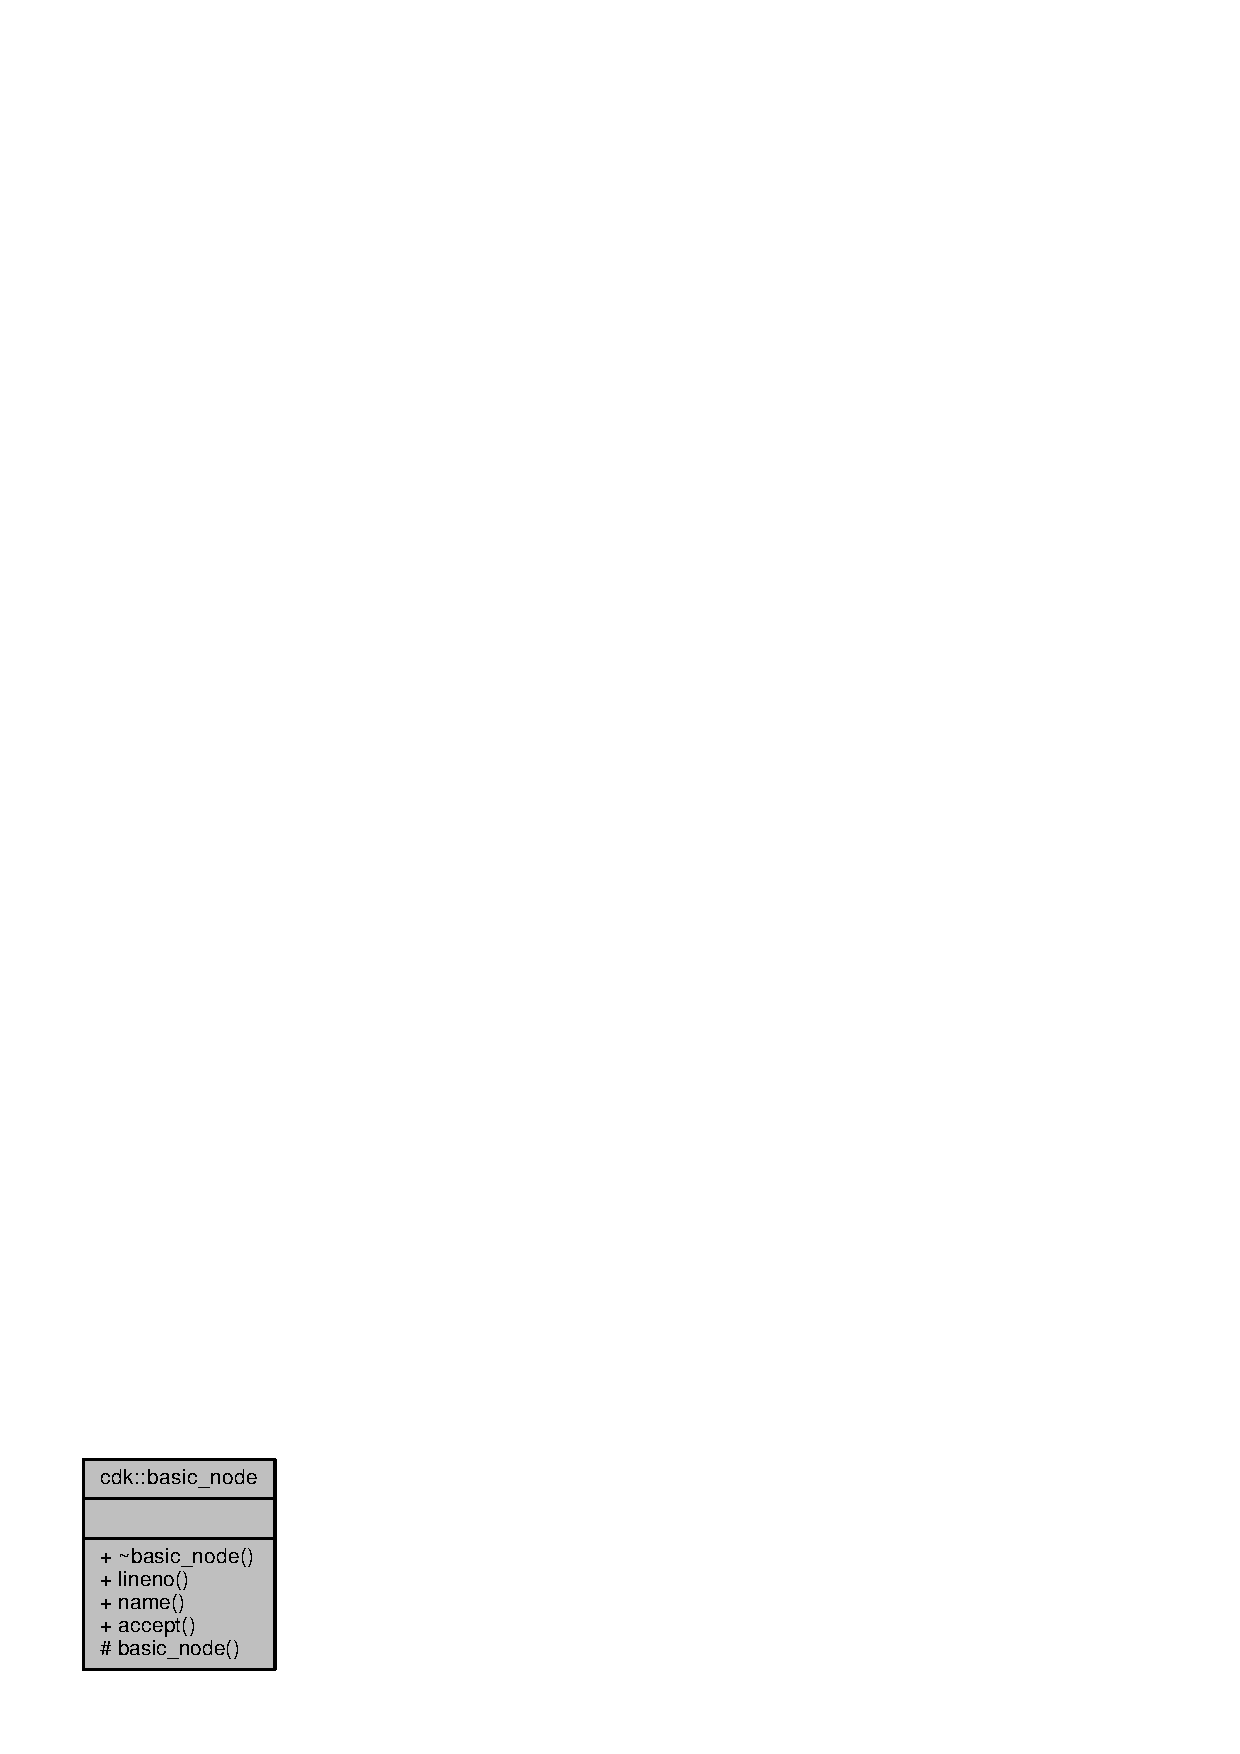
\includegraphics[width=136pt]{classcdk_1_1basic__node__coll__graph}
\end{center}
\end{figure}
\subsection*{Public Member Functions}
\begin{DoxyCompactItemize}
\item 
int {\bf lineno} () const 
\item 
std\+::string {\bf name} () const 
\item 
virtual void {\bf accept} ({\bf basic\+\_\+ast\+\_\+visitor} $\ast$sp, int level)=0
\end{DoxyCompactItemize}
\subsection*{Protected Member Functions}
\begin{DoxyCompactItemize}
\item 
{\bf basic\+\_\+node} (int {\bf lineno})
\end{DoxyCompactItemize}


\subsection{Detailed Description}
Class for describing A\+S\+T nodes. This is an abstract class and forms the root of the node hierarchy. The node hierarchy is organized in a structure according to the {\itshape Composite} design pattern\+: class {\ttfamily node} is the root of the hierarchy; class {\ttfamily simple} is a template for leaves holding simple (atomic) types; {\ttfamily composite} represents the recursive structure. Note that other recursion classes are possible by extending any of the classes in this family. 

Definition at line 21 of file basic\+\_\+node.\+h.



\subsection{Constructor \& Destructor Documentation}
\index{cdk\+::basic\+\_\+node@{cdk\+::basic\+\_\+node}!basic\+\_\+node@{basic\+\_\+node}}
\index{basic\+\_\+node@{basic\+\_\+node}!cdk\+::basic\+\_\+node@{cdk\+::basic\+\_\+node}}
\subsubsection[{basic\+\_\+node}]{\setlength{\rightskip}{0pt plus 5cm}cdk\+::basic\+\_\+node\+::basic\+\_\+node (
\begin{DoxyParamCaption}
\item[{int}]{lineno}
\end{DoxyParamCaption}
)\hspace{0.3cm}{\ttfamily [inline]}, {\ttfamily [protected]}}\label{classcdk_1_1basic__node_a4e09fec517e3a83503852de9e4fd5d72}
Simple constructor.


\begin{DoxyParams}{Parameters}
{\em lineno} & the source code line number corresponding to the node \\
\hline
\end{DoxyParams}


Definition at line 30 of file basic\+\_\+node.\+h.



\subsection{Member Function Documentation}
\index{cdk\+::basic\+\_\+node@{cdk\+::basic\+\_\+node}!accept@{accept}}
\index{accept@{accept}!cdk\+::basic\+\_\+node@{cdk\+::basic\+\_\+node}}
\subsubsection[{accept}]{\setlength{\rightskip}{0pt plus 5cm}virtual void cdk\+::basic\+\_\+node\+::accept (
\begin{DoxyParamCaption}
\item[{{\bf basic\+\_\+ast\+\_\+visitor} $\ast$}]{sp, }
\item[{int}]{level}
\end{DoxyParamCaption}
)\hspace{0.3cm}{\ttfamily [pure virtual]}}\label{classcdk_1_1basic__node_ab38adcbc95c46b809961278afae3bf05}
Every node must provide this method.


\begin{DoxyParams}{Parameters}
{\em sp} & semantic processor visitor \\
\hline
{\em level} & syntactic tree level \\
\hline
\end{DoxyParams}


Implemented in {\bf cdk\+::sequence\+\_\+node} \doxyref{}{p.}{classcdk_1_1sequence__node_a65774c75d4f946c18222043a14968190}, {\bf cdk\+::composite\+\_\+node} \doxyref{}{p.}{classcdk_1_1composite__node_af7ac243ab23b1204c44010cf42ef14a2}, {\bf cdk\+::data\+\_\+node} \doxyref{}{p.}{classcdk_1_1data__node_a9d6d6f56201fdfbe965ec399ced60df8}, {\bf cdk\+::if\+\_\+else\+\_\+node} \doxyref{}{p.}{classcdk_1_1if__else__node_a348ea45d822a94125a12156c92db48a0}, {\bf cdk\+::nil\+\_\+node} \doxyref{}{p.}{classcdk_1_1nil__node_a98fe1eb1acb00d40f91a75a18db2e86d}, {\bf cdk\+::identifier\+\_\+node} \doxyref{}{p.}{classcdk_1_1identifier__node_aab81ccb83be770047771dda4c59b0568}, {\bf cdk\+::string\+\_\+node} \doxyref{}{p.}{classcdk_1_1string__node_a8ddaf8a19a75e2ff892eadd1606cb16f}, {\bf cdk\+::if\+\_\+node} \doxyref{}{p.}{classcdk_1_1if__node_a3fee89ddd665238ed4db37fd73d01d81}, {\bf cdk\+::while\+\_\+node} \doxyref{}{p.}{classcdk_1_1while__node_a7599c47777a5423a5889c3e708bb13bb}, {\bf cdk\+::eq\+\_\+node} \doxyref{}{p.}{classcdk_1_1eq__node_ac874f2c13fc2f66ce23b08d99594368e}, {\bf cdk\+::add\+\_\+node} \doxyref{}{p.}{classcdk_1_1add__node_a5a0a7fd1aacfcf589233c9b1cdda59d1}, {\bf cdk\+::ge\+\_\+node} \doxyref{}{p.}{classcdk_1_1ge__node_a758ad0281c1e925aab356d757bedce40}, {\bf cdk\+::gt\+\_\+node} \doxyref{}{p.}{classcdk_1_1gt__node_ab1104710ad583f4b13d397bf33b2f9f5}, {\bf cdk\+::le\+\_\+node} \doxyref{}{p.}{classcdk_1_1le__node_a4d3a01246f47dcb95ab7535a9047c9d6}, {\bf cdk\+::lt\+\_\+node} \doxyref{}{p.}{classcdk_1_1lt__node_a6af8ca3130c12e7a38860c9e92aaaa97}, {\bf cdk\+::mod\+\_\+node} \doxyref{}{p.}{classcdk_1_1mod__node_a990120f568275fb78d9adf66ec46434a}, {\bf cdk\+::mul\+\_\+node} \doxyref{}{p.}{classcdk_1_1mul__node_a82daadfc3194683a75c2e0630d09318d}, {\bf cdk\+::ne\+\_\+node} \doxyref{}{p.}{classcdk_1_1ne__node_a66ac549e9cc152c1d4c23dfe0c3c3830}, {\bf cdk\+::sub\+\_\+node} \doxyref{}{p.}{classcdk_1_1sub__node_a6200490aef72dc9483ac91047ba78e12}, {\bf cdk\+::div\+\_\+node} \doxyref{}{p.}{classcdk_1_1div__node_a18fdb1b825aeba112a607964f3901a6d}, {\bf cdk\+::double\+\_\+node} \doxyref{}{p.}{classcdk_1_1double__node_a3338941e9e94a4f88df4a418092c1ec8}, {\bf cdk\+::integer\+\_\+node} \doxyref{}{p.}{classcdk_1_1integer__node_a6b47d4c572b80bbaed62604a8c68788d}, and {\bf cdk\+::neg\+\_\+node} \doxyref{}{p.}{classcdk_1_1neg__node_ac49b8a32b9edaccfe38000cdb23d44c2}.

\index{cdk\+::basic\+\_\+node@{cdk\+::basic\+\_\+node}!lineno@{lineno}}
\index{lineno@{lineno}!cdk\+::basic\+\_\+node@{cdk\+::basic\+\_\+node}}
\subsubsection[{lineno}]{\setlength{\rightskip}{0pt plus 5cm}int cdk\+::basic\+\_\+node\+::lineno (
\begin{DoxyParamCaption}
{}
\end{DoxyParamCaption}
) const\hspace{0.3cm}{\ttfamily [inline]}}\label{classcdk_1_1basic__node_a4750afc3539d2b8f53ca74dbdd181a02}
\begin{DoxyReturn}{Returns}
the line number of the corresponding source code 
\end{DoxyReturn}


Definition at line 40 of file basic\+\_\+node.\+h.

\index{cdk\+::basic\+\_\+node@{cdk\+::basic\+\_\+node}!name@{name}}
\index{name@{name}!cdk\+::basic\+\_\+node@{cdk\+::basic\+\_\+node}}
\subsubsection[{name}]{\setlength{\rightskip}{0pt plus 5cm}std\+::string cdk\+::basic\+\_\+node\+::name (
\begin{DoxyParamCaption}
{}
\end{DoxyParamCaption}
) const\hspace{0.3cm}{\ttfamily [inline]}}\label{classcdk_1_1basic__node_a181c07863b3f40eaabac9a5e69160cab}
\begin{DoxyReturn}{Returns}
the name of the node's class 
\end{DoxyReturn}


Definition at line 47 of file basic\+\_\+node.\+h.



The documentation for this class was generated from the following file\+:\begin{DoxyCompactItemize}
\item 
ast/basic\+\_\+node.\+h\end{DoxyCompactItemize}

\section{cdk\+:\+:basic\+\_\+parser Class Reference}
\label{classcdk_1_1basic__parser}\index{cdk\+::basic\+\_\+parser@{cdk\+::basic\+\_\+parser}}


Inheritance diagram for cdk\+:\+:basic\+\_\+parser\+:
\nopagebreak
\begin{figure}[H]
\begin{center}
\leavevmode
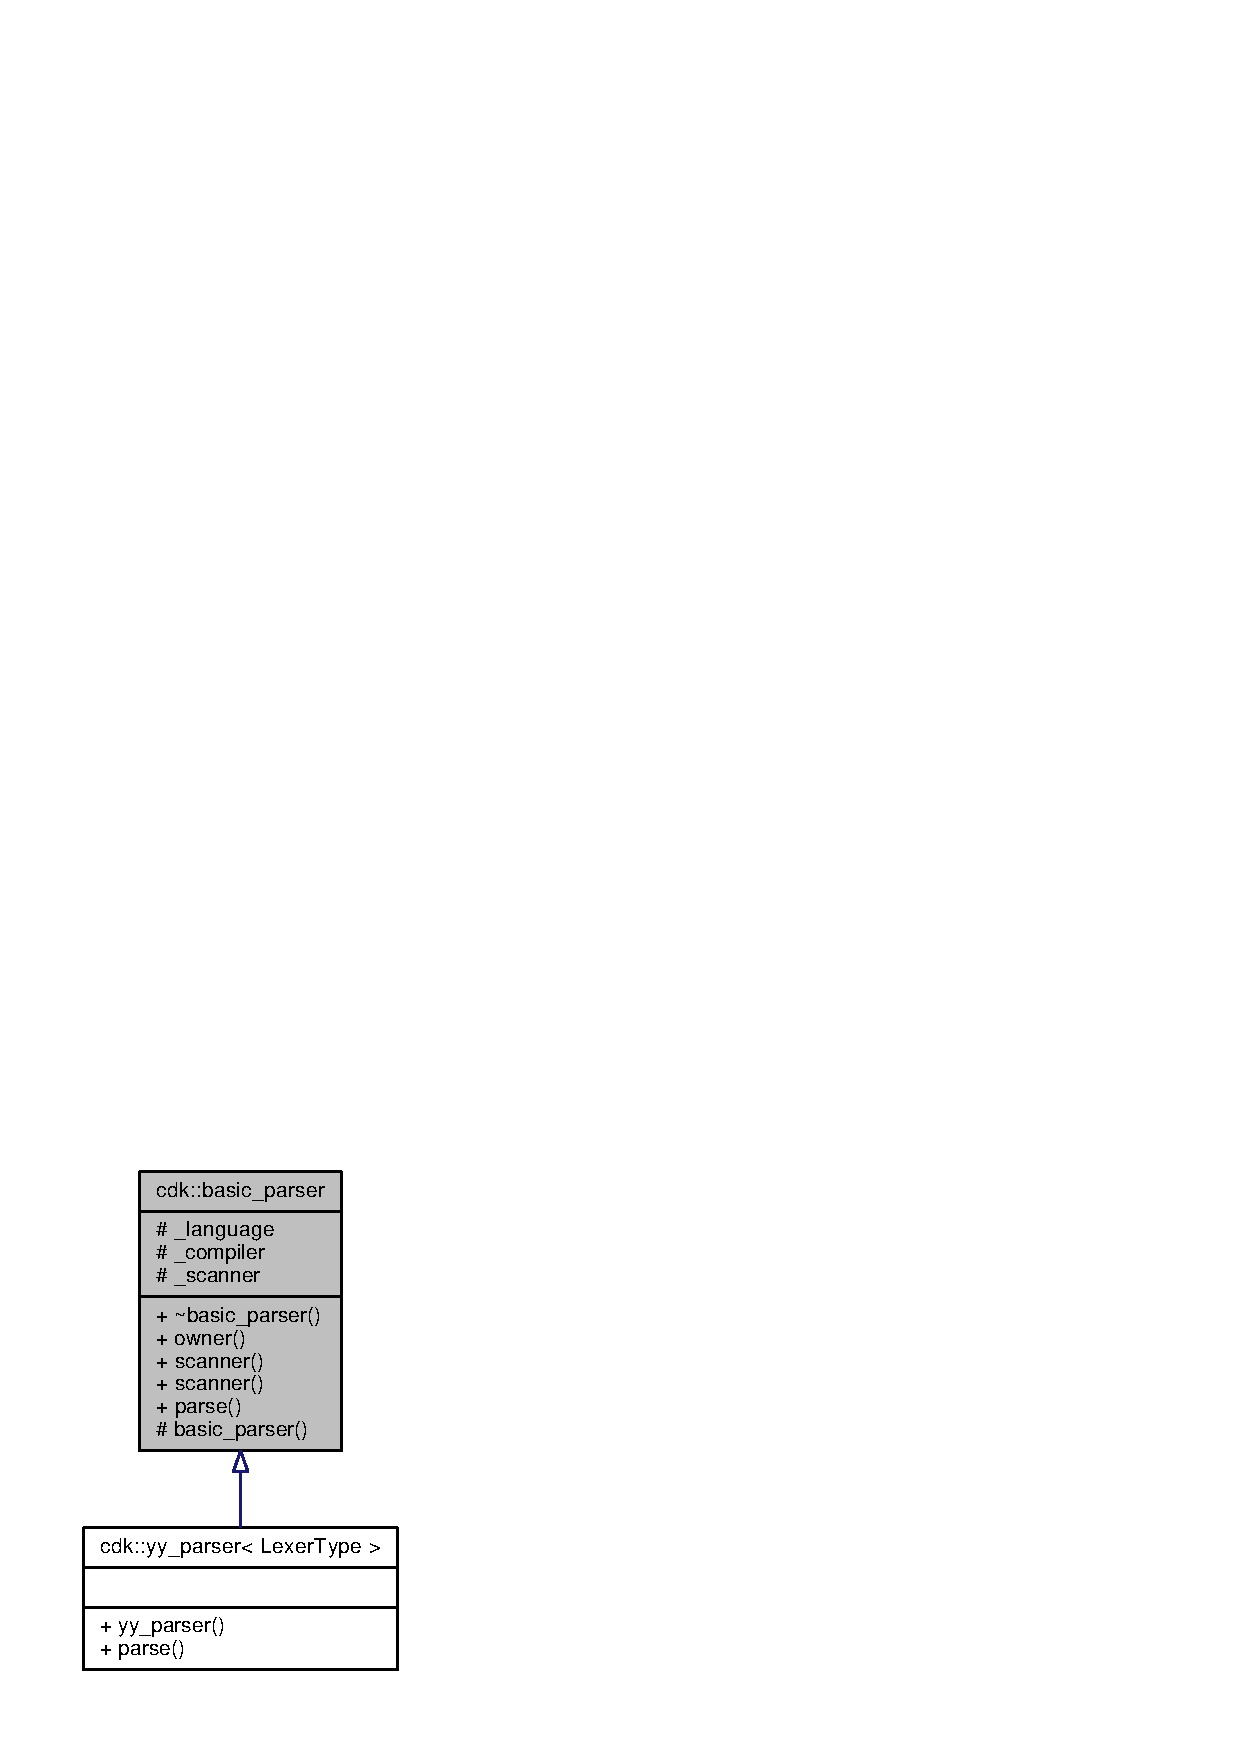
\includegraphics[width=195pt]{classcdk_1_1basic__parser__inherit__graph}
\end{center}
\end{figure}


Collaboration diagram for cdk\+:\+:basic\+\_\+parser\+:
\nopagebreak
\begin{figure}[H]
\begin{center}
\leavevmode
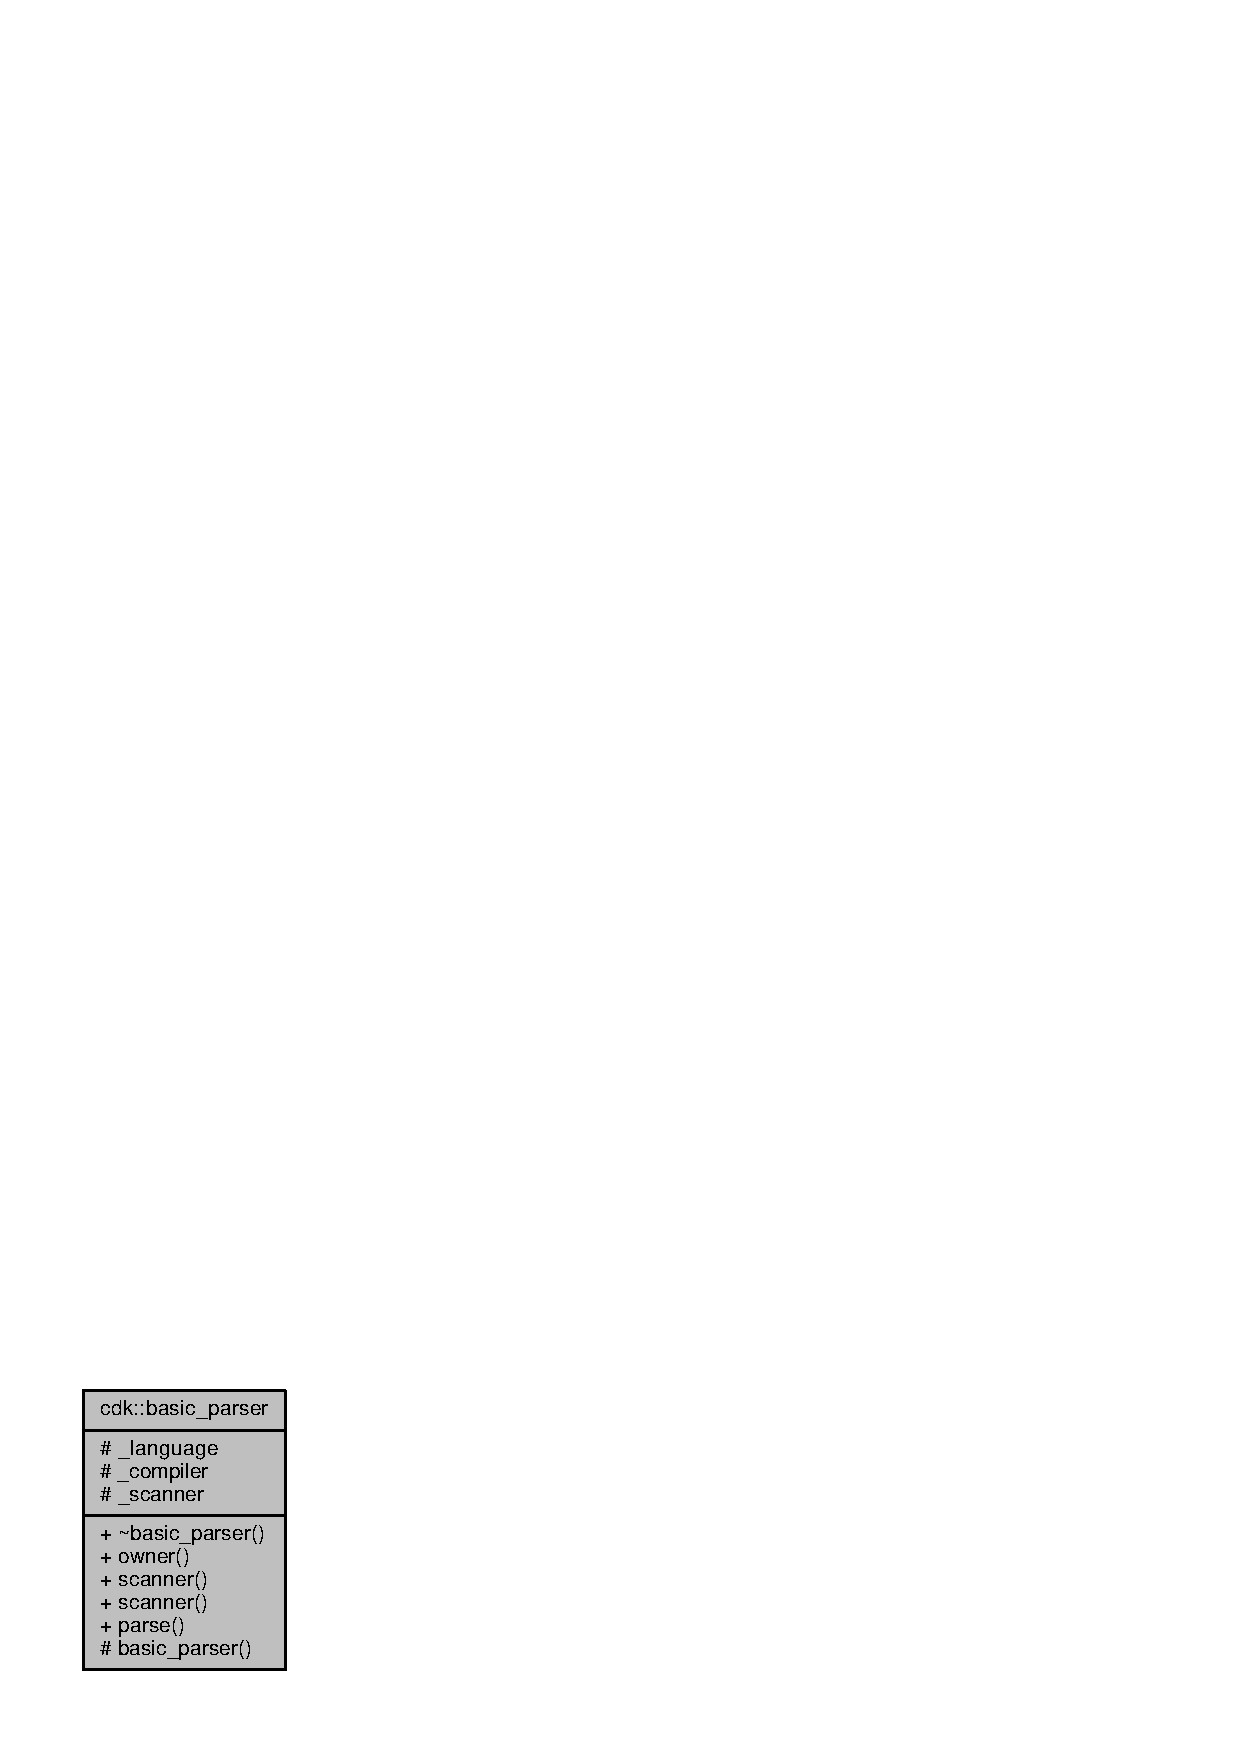
\includegraphics[width=141pt]{classcdk_1_1basic__parser__coll__graph}
\end{center}
\end{figure}
\subsection*{Public Member Functions}
\begin{DoxyCompactItemize}
\item 
std\+::shared\+\_\+ptr$<$ {\bf compiler} $>$ {\bfseries owner} ()\label{classcdk_1_1basic__parser_a536c2274f7b00c0e17858b0ee1a400d6}

\item 
std\+::shared\+\_\+ptr$<$ {\bf basic\+\_\+scanner} $>$ {\bfseries scanner} ()\label{classcdk_1_1basic__parser_a68543c111a7fef48ebe70c47b02ead09}

\item 
void {\bfseries scanner} (std\+::shared\+\_\+ptr$<$ {\bf basic\+\_\+scanner} $>$ scanner)\label{classcdk_1_1basic__parser_acc2215d959879e6fbac2f3e505c6bc03}

\item 
virtual int {\bf parse} ()=0
\end{DoxyCompactItemize}
\subsection*{Protected Member Functions}
\begin{DoxyCompactItemize}
\item 
{\bfseries basic\+\_\+parser} (const std\+::string \&language, std\+::shared\+\_\+ptr$<$ {\bf basic\+\_\+scanner} $>$ scanner)\label{classcdk_1_1basic__parser_a11506116556681fc7fbfe4a974ec0b34}

\end{DoxyCompactItemize}
\subsection*{Protected Attributes}
\begin{DoxyCompactItemize}
\item 
const std\+::string {\bfseries \+\_\+language} = \char`\"{}\char`\"{}\label{classcdk_1_1basic__parser_a1c97f24997ae2bceeae4822e32a449e4}

\item 
std\+::shared\+\_\+ptr$<$ {\bf compiler} $>$ {\bfseries \+\_\+compiler} = nullptr\label{classcdk_1_1basic__parser_a1071aa82583cd806add631b8453fbfb1}

\item 
std\+::shared\+\_\+ptr$<$ {\bf basic\+\_\+scanner} $>$ {\bfseries \+\_\+scanner} = nullptr\label{classcdk_1_1basic__parser_aa88b520cd9bc71be71c9ad9dedbd9895}

\end{DoxyCompactItemize}
\subsection*{Friends}
\begin{DoxyCompactItemize}
\item 
class {\bfseries compiler}\label{classcdk_1_1basic__parser_a6450bc9182feebc4fe52fbf86fa0ba40}

\end{DoxyCompactItemize}


\subsection{Detailed Description}


Definition at line 13 of file basic\+\_\+parser.\+h.



\subsection{Member Function Documentation}
\index{cdk\+::basic\+\_\+parser@{cdk\+::basic\+\_\+parser}!parse@{parse}}
\index{parse@{parse}!cdk\+::basic\+\_\+parser@{cdk\+::basic\+\_\+parser}}
\subsubsection[{parse}]{\setlength{\rightskip}{0pt plus 5cm}virtual int cdk\+::basic\+\_\+parser\+::parse (
\begin{DoxyParamCaption}
{}
\end{DoxyParamCaption}
)\hspace{0.3cm}{\ttfamily [pure virtual]}}\label{classcdk_1_1basic__parser_a974c94ef048509a80bd042ee9c783513}
Parse algorithm\+: the compiler object stores the result. 
\begin{DoxyParams}{Parameters}
{\em compiler} & the compiler object this parser belongs to. \\
\hline
\end{DoxyParams}
\begin{DoxyReturn}{Returns}
true if the operation is successful 
\end{DoxyReturn}


Implemented in {\bf cdk\+::yy\+\_\+parser$<$ Lexer\+Type $>$} \doxyref{}{p.}{classcdk_1_1yy__parser_a998a98a7b38a6772fb24ae0eeb87ef17}.



The documentation for this class was generated from the following file\+:\begin{DoxyCompactItemize}
\item 
basic\+\_\+parser.\+h\end{DoxyCompactItemize}

\section{cdk\+:\+:basic\+\_\+postfix\+\_\+emitter Class Reference}
\label{classcdk_1_1basic__postfix__emitter}\index{cdk\+::basic\+\_\+postfix\+\_\+emitter@{cdk\+::basic\+\_\+postfix\+\_\+emitter}}


{\ttfamily \#include $<$basic\+\_\+postfix\+\_\+emitter.\+h$>$}



Inheritance diagram for cdk\+:\+:basic\+\_\+postfix\+\_\+emitter\+:
\nopagebreak
\begin{figure}[H]
\begin{center}
\leavevmode
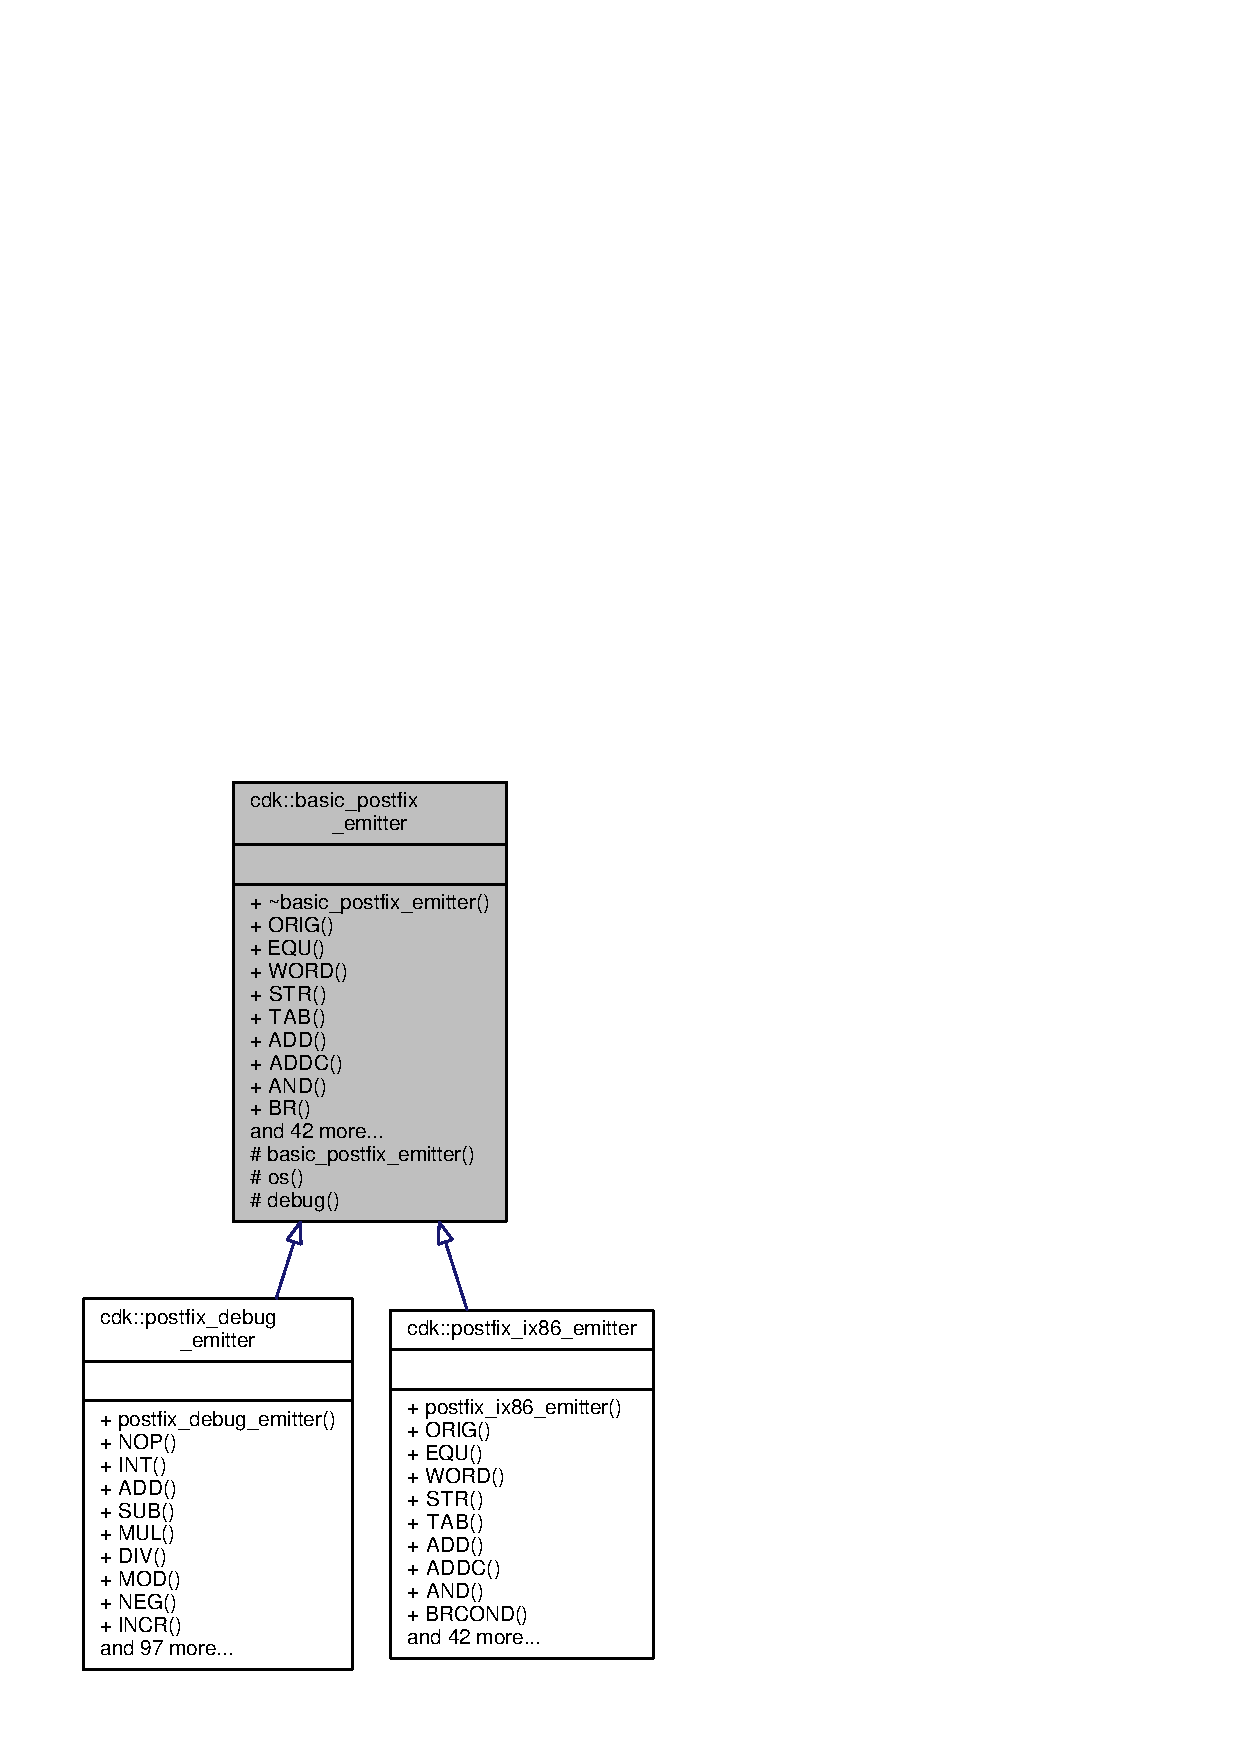
\includegraphics[width=318pt]{classcdk_1_1basic__postfix__emitter__inherit__graph}
\end{center}
\end{figure}


Collaboration diagram for cdk\+:\+:basic\+\_\+postfix\+\_\+emitter\+:
\nopagebreak
\begin{figure}[H]
\begin{center}
\leavevmode
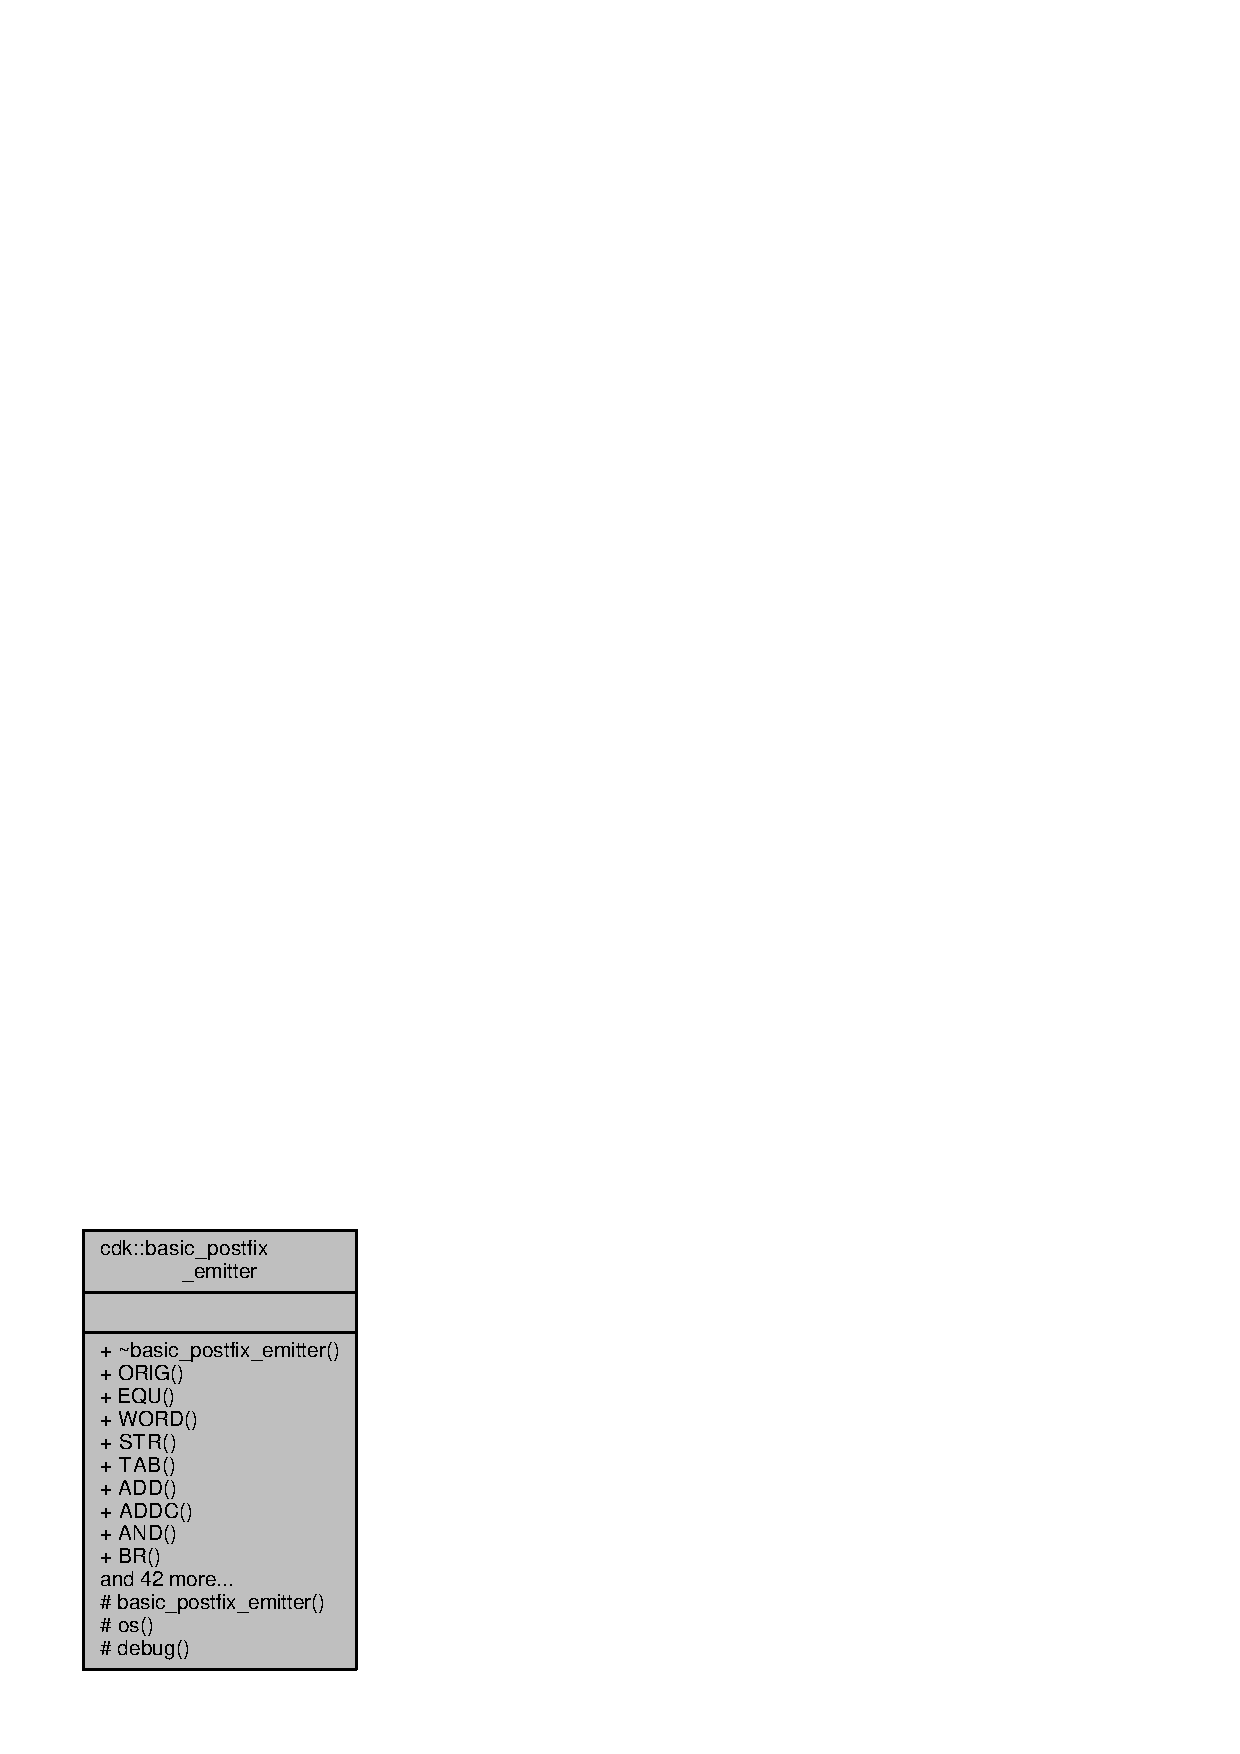
\includegraphics[width=175pt]{classcdk_1_1basic__postfix__emitter__coll__graph}
\end{center}
\end{figure}
\subsection*{Public Member Functions}
\begin{DoxyCompactItemize}
\item 
virtual {\bf $\sim$basic\+\_\+postfix\+\_\+emitter} ()
\item 
virtual void {\bfseries O\+R\+I\+G} (int)=0\label{classcdk_1_1basic__postfix__emitter_af66165e8f4e5a0fe4bf077bfe3e9611c}

\item 
virtual void {\bfseries E\+Q\+U} (std\+::string, int)=0\label{classcdk_1_1basic__postfix__emitter_ae7488e587652910e45409f82be277402}

\item 
virtual void {\bfseries W\+O\+R\+D} (std\+::string, int)=0\label{classcdk_1_1basic__postfix__emitter_a0beb8e87e629adf3ab248ec8c122f2a9}

\item 
virtual void {\bfseries S\+T\+R} (std\+::string, std\+::string)=0\label{classcdk_1_1basic__postfix__emitter_a561510fb8b3ebd8d7d7f5e07255c374d}

\item 
virtual void {\bfseries T\+A\+B} (std\+::string, int)=0\label{classcdk_1_1basic__postfix__emitter_adfc8362edf35b90a2a06d5db3e38a40e}

\item 
virtual void {\bfseries A\+D\+D} ()=0\label{classcdk_1_1basic__postfix__emitter_a166a0afe31c5b1249b45c8f909bad6a1}

\item 
virtual void {\bfseries A\+D\+D\+C} ()=0\label{classcdk_1_1basic__postfix__emitter_ad2fb5791a8a36c00d807efd85ba7508d}

\item 
virtual void {\bfseries A\+N\+D} ()=0\label{classcdk_1_1basic__postfix__emitter_a0e1eed9bc80ca1ace031793aeca088d2}

\item 
virtual void {\bfseries B\+R} (std\+::string)=0\label{classcdk_1_1basic__postfix__emitter_a8f6b549211dd46dd6edb74166beccaee}

\item 
virtual void {\bfseries B\+R\+C\+O\+N\+D} (std\+::string, std\+::string)=0\label{classcdk_1_1basic__postfix__emitter_afbfe6647474a3338bec171b44ac2728b}

\item 
virtual void {\bfseries C\+A\+L\+L} (std\+::string)=0\label{classcdk_1_1basic__postfix__emitter_afce2babf830192bb7c008202d94c0b1e}

\item 
virtual void {\bfseries C\+A\+L\+L\+C\+O\+N\+D} (std\+::string, std\+::string)=0\label{classcdk_1_1basic__postfix__emitter_ab94c46ed1d4702a2aa3b709aa30a53a6}

\item 
virtual void {\bfseries C\+L\+C} ()=0\label{classcdk_1_1basic__postfix__emitter_abd5772172ea0d91ed4da1bd8ee7b2fb5}

\item 
virtual void {\bfseries C\+M\+C} ()=0\label{classcdk_1_1basic__postfix__emitter_a5fe7d27a6bab7a18ee0c0a1b33db119f}

\item 
virtual void {\bfseries C\+M\+P} ()=0\label{classcdk_1_1basic__postfix__emitter_a2f5572c7a7ead89bf463f779826a9aa2}

\item 
virtual void {\bfseries C\+O\+M} ()=0\label{classcdk_1_1basic__postfix__emitter_ad5fa32f0a8a042074a360fe3ad6131ea}

\item 
virtual void {\bfseries D\+E\+C} ()=0\label{classcdk_1_1basic__postfix__emitter_af2249fe5f5dffd58e236e8a92ecce588}

\item 
virtual void {\bfseries D\+I\+V} ()=0\label{classcdk_1_1basic__postfix__emitter_af91bf2f2e22ce0584f7ed2d1ac86784f}

\item 
virtual void {\bfseries D\+S\+I} ()=0\label{classcdk_1_1basic__postfix__emitter_a9d5bdd7531ea1199b37cc04664cb7c52}

\item 
virtual void {\bfseries E\+N\+I} ()=0\label{classcdk_1_1basic__postfix__emitter_a58f2c247bd1e955ab49ba2890a4cca1c}

\item 
virtual void {\bfseries I\+N\+C} ()=0\label{classcdk_1_1basic__postfix__emitter_a0ecfc996fe98accfd7ce91593543adee}

\item 
virtual void {\bfseries I\+N\+T} (int)=0\label{classcdk_1_1basic__postfix__emitter_a7696ceafbfaa94b56e517005c4451d18}

\item 
virtual void {\bfseries J\+M\+P} (std\+::string)=0\label{classcdk_1_1basic__postfix__emitter_a6b69b6284da7299d71b0294ebbbaef60}

\item 
virtual void {\bfseries J\+M\+P\+C\+O\+N\+D} (std\+::string, std\+::string)=0\label{classcdk_1_1basic__postfix__emitter_ab0e8c60b877df9c721b08b156f83fd0c}

\item 
virtual void {\bfseries M\+O\+V} ()=0\label{classcdk_1_1basic__postfix__emitter_a4480ffe2d77a5ac4f8502be600ac08d3}

\item 
virtual void {\bfseries M\+U\+L} ()=0\label{classcdk_1_1basic__postfix__emitter_a1b4edc79e9074688feb51609f1b8137b}

\item 
virtual void {\bfseries M\+V\+B\+H} ()=0\label{classcdk_1_1basic__postfix__emitter_a584fefb1f335e4b9ba04b8844cdc3e21}

\item 
virtual void {\bfseries M\+V\+B\+L} ()=0\label{classcdk_1_1basic__postfix__emitter_ae60e5813a739d43884be425baf152f72}

\item 
virtual void {\bfseries N\+E\+G} ()=0\label{classcdk_1_1basic__postfix__emitter_abcf3ea8d995b9c898e8b97920c1f3d19}

\item 
virtual void {\bfseries N\+O\+P} ()=0\label{classcdk_1_1basic__postfix__emitter_a8b45caa490a5b0aef1aa2a25cd3a163e}

\item 
virtual void {\bfseries O\+R} ()=0\label{classcdk_1_1basic__postfix__emitter_a8bffc779f5bc6b0878adc68aa19763f8}

\item 
virtual void {\bfseries P\+O\+P} ()=0\label{classcdk_1_1basic__postfix__emitter_a87f4067fc2c1fc7e5cb4676a0cd691e5}

\item 
virtual void {\bfseries P\+U\+S\+H} (int value)=0\label{classcdk_1_1basic__postfix__emitter_ae330fba22afd103ef31ec578b3044064}

\item 
virtual void {\bfseries R\+E\+T} ()=0\label{classcdk_1_1basic__postfix__emitter_a80e164209c2b470c46040e12c8c796b2}

\item 
virtual void {\bfseries R\+E\+T\+N} (int)=0\label{classcdk_1_1basic__postfix__emitter_a49d4847065b9b9c8364949b5d07e62f1}

\item 
virtual void {\bfseries R\+O\+L} (int)=0\label{classcdk_1_1basic__postfix__emitter_aeede745ec6d7d8a06226ccbaecfc3a21}

\item 
virtual void {\bfseries R\+O\+L\+C} (int)=0\label{classcdk_1_1basic__postfix__emitter_aa34bacf7cb787b8be7bed0a73e55ec64}

\item 
virtual void {\bfseries R\+O\+R} (int)=0\label{classcdk_1_1basic__postfix__emitter_a16c566ba60778cb964c1df8c3cd50bde}

\item 
virtual void {\bfseries R\+O\+R\+C} (int)=0\label{classcdk_1_1basic__postfix__emitter_ae1d0e7b0eb4234b694d7ac3e2bf17b9e}

\item 
virtual void {\bfseries R\+T\+I} ()=0\label{classcdk_1_1basic__postfix__emitter_adedd584bec1b349acaeeea2d6ddd0907}

\item 
virtual void {\bfseries S\+H\+L} (int)=0\label{classcdk_1_1basic__postfix__emitter_a21d9b8518e41b200699c5f84012ee705}

\item 
virtual void {\bfseries S\+H\+L\+A} (int)=0\label{classcdk_1_1basic__postfix__emitter_a9227abe7c4a415b67aac9e38affb90a9}

\item 
virtual void {\bfseries S\+H\+R} (int)=0\label{classcdk_1_1basic__postfix__emitter_a06a2289095b1a45e1dbe1575cd78cc03}

\item 
virtual void {\bfseries S\+H\+R\+A} (int)=0\label{classcdk_1_1basic__postfix__emitter_a8351461f83386d6865a3ff1b8a5f6c24}

\item 
virtual void {\bfseries S\+T\+C} ()=0\label{classcdk_1_1basic__postfix__emitter_a7476ce1ea0dd76b4250e4406f14ef164}

\item 
virtual void {\bfseries S\+U\+B} ()=0\label{classcdk_1_1basic__postfix__emitter_af396160c6fe8d66e96244b825e0a6243}

\item 
virtual void {\bfseries S\+U\+B\+B} ()=0\label{classcdk_1_1basic__postfix__emitter_a7a96b8a16148b51b2f6f04d9e80226f6}

\item 
virtual void {\bfseries T\+E\+S\+T} ()=0\label{classcdk_1_1basic__postfix__emitter_a944645da0e07dddaaab64806168dbc81}

\item 
virtual void {\bfseries X\+C\+H} ()=0\label{classcdk_1_1basic__postfix__emitter_ae383aa17f0100e5888be13f82df561c0}

\item 
virtual void {\bfseries X\+O\+R} ()=0\label{classcdk_1_1basic__postfix__emitter_a4f81d834e05b994699cffbee1f3e3aad}

\item 
virtual void {\bfseries L\+A\+B\+E\+L} (std\+::string)=0\label{classcdk_1_1basic__postfix__emitter_a538fc78f19108ec1635246825ecb16fa}

\end{DoxyCompactItemize}
\subsection*{Protected Member Functions}
\begin{DoxyCompactItemize}
\item 
{\bfseries basic\+\_\+postfix\+\_\+emitter} (std\+::shared\+\_\+ptr$<$ {\bf compiler} $>$ \&{\bf compiler})\label{classcdk_1_1basic__postfix__emitter_acaf970d10f218a088bd57ca6bcadce35}

\item 
std\+::ostream \& {\bfseries os} ()\label{classcdk_1_1basic__postfix__emitter_a34b69125c2b35e846461de6328894166}

\item 
bool {\bfseries debug} ()\label{classcdk_1_1basic__postfix__emitter_ab8a379fd593474bc165f8187d831affd}

\end{DoxyCompactItemize}


\subsection{Detailed Description}
The postfix code emitter defines an interface to be used by semantic analysers, as defined by the strategy design pattern. Specific implementations will provide the realization of the postfix commands for a particular target machine.

\paragraph*{Rotation and shift instructions}

Shift and rotation operations have as maximum value the number of bits of the underlying processor register (32 bits in a ix86-\/family processor). Safe operation for values above is not guaranteed.

These operations use two values from the stack\+: the value at the top specifies the number of bits to rotate/shift; the second from the top is the value to be rotated/shifted.

\paragraph*{Logical instructions}

Logical instructions perform logical operations using the elements at the top of the stack. Arguments are taken from the stack, the result is put on the stack.

\paragraph*{Type conversion instructions}

Type conversion instructions perform elementary type conversions. The conversions are from and to integers and simple and double precision floating point values.

\paragraph*{Integer comparison instructions}

The comparison instructions are binary operations that leave at the top of the stack 0 (zero) or 1 (one), depending on the result result of the comparison\+: respectively, {\ttfamily false} or {\ttfamily true}. The value may be directly used to perform conditional jumps (e.\+g., J\+Z, J\+N\+Z), that use the value of the top of the stack instead of relying on special processor registers ({\itshape flags}).

\paragraph*{Function definition instructions}

In a stack machine the arguments for a function call are already in the stack. Thus, it is not necessary to put them there (it is enough not to remove them). When building functions that conform to the C calling convetions, those arguments are destroyed by the caller, {\itshape after} the return of the callee, using {\ttfamily T\+R\+A\+S\+H}, stating the total size (i.\+e., for all arguments). Regarding the callee, it must create a distinct activation register {\ttfamily E\+N\+T\+E\+R} or {\ttfamily S\+T\+A\+R\+T}) and, when no longer needed, destroy it ({\ttfamily L\+E\+A\+V\+E}). The latter action must be performed immediately before returning control to the caller.

Similarly, to return values from a function, the callee must call {\ttfamily P\+O\+P} to store the return value in the accumulator register, so that it survives the destruction of the invocation context. The caller must call {\ttfamily P\+U\+S\+H}, to put the accumulator in the stack. An analogous procedure is valid for {\ttfamily D\+P\+O\+P/\+D\+P\+U\+S\+H} (for double precision floating point return values).

\paragraph*{Addressing instructions}

Note [{\itshape 4}] that these operations (A\+D\+D\+R, L\+O\+C\+A\+L) put at the top of the stack the symbol's address, independently of its origin. O endereço pode posteriormente ser utilizado como ponteiro, obtido o valor nesse endereço (L\+O\+A\+D) ou guardar um valor nesse endereço (S\+T\+O\+R\+E). No entanto, nas duas últimas situações, devido à frequência com que ocorrem e o número de ciclos de relógio que levam a executar, podem ser substituídas com vantagem pela operações descritas em [{\itshape 10}].

\char`\"{}\+Quick opcodes\char`\"{} are shortcuts for groups of operations commonly used together. These opcodes may be made efficient by implementing them in different ways than the original set of high-\/level operations would suggest, i.\+e., the code generated by {\ttfamily A\+D\+D\+R\+V} may be more efficient than the code generated by {\ttfamily A\+D\+D\+R} followed by {\ttfamily L\+O\+A\+D}. Nevertheless, the outcome is the same.

\paragraph*{Load instructions}

The load instructions assume that the top of the stack contains an address pointing to the data to be read. Each load instruction will replace the address at the top of the stack with the contents of the position it points to. Load instructions differ only in what they load.

\paragraph*{Store instructions}

Store instructions assume the stack contains at the top the address where data is to be stored. That data is in the stack, immediately after (below) the address. Store instructions differ only in what they store.

\paragraph*{Labels}

In a declaration of a symbol common to more than one module, other modules may also contain common or external declarations. Nevertheless, only one initialized declaration is allowed. Declarations need not be associated with any particular segments.

In a declaration common to several modules, any number of modules may contain common or external declarations, but only one of them may contain an initialized declaration. A declaration does not need to be specified in a specific segment. 

Definition at line 107 of file basic\+\_\+postfix\+\_\+emitter.\+h.



\subsection{Constructor \& Destructor Documentation}
\index{cdk\+::basic\+\_\+postfix\+\_\+emitter@{cdk\+::basic\+\_\+postfix\+\_\+emitter}!````~basic\+\_\+postfix\+\_\+emitter@{$\sim$basic\+\_\+postfix\+\_\+emitter}}
\index{````~basic\+\_\+postfix\+\_\+emitter@{$\sim$basic\+\_\+postfix\+\_\+emitter}!cdk\+::basic\+\_\+postfix\+\_\+emitter@{cdk\+::basic\+\_\+postfix\+\_\+emitter}}
\subsubsection[{$\sim$basic\+\_\+postfix\+\_\+emitter}]{\setlength{\rightskip}{0pt plus 5cm}virtual cdk\+::basic\+\_\+postfix\+\_\+emitter\+::$\sim$basic\+\_\+postfix\+\_\+emitter (
\begin{DoxyParamCaption}
{}
\end{DoxyParamCaption}
)\hspace{0.3cm}{\ttfamily [inline]}, {\ttfamily [virtual]}}\label{classcdk_1_1basic__postfix__emitter_a4379176e34cbebf1ed583cf1666a3273}
Destructor\+: the only action is to flush the output stream. 

Definition at line 129 of file basic\+\_\+postfix\+\_\+emitter.\+h.



The documentation for this class was generated from the following file\+:\begin{DoxyCompactItemize}
\item 
emitters/basic\+\_\+postfix\+\_\+emitter.\+h\end{DoxyCompactItemize}

\section{cdk\+:\+:basic\+\_\+scanner Class Reference}
\label{classcdk_1_1basic__scanner}\index{cdk\+::basic\+\_\+scanner@{cdk\+::basic\+\_\+scanner}}


Inheritance diagram for cdk\+:\+:basic\+\_\+scanner\+:
\nopagebreak
\begin{figure}[H]
\begin{center}
\leavevmode
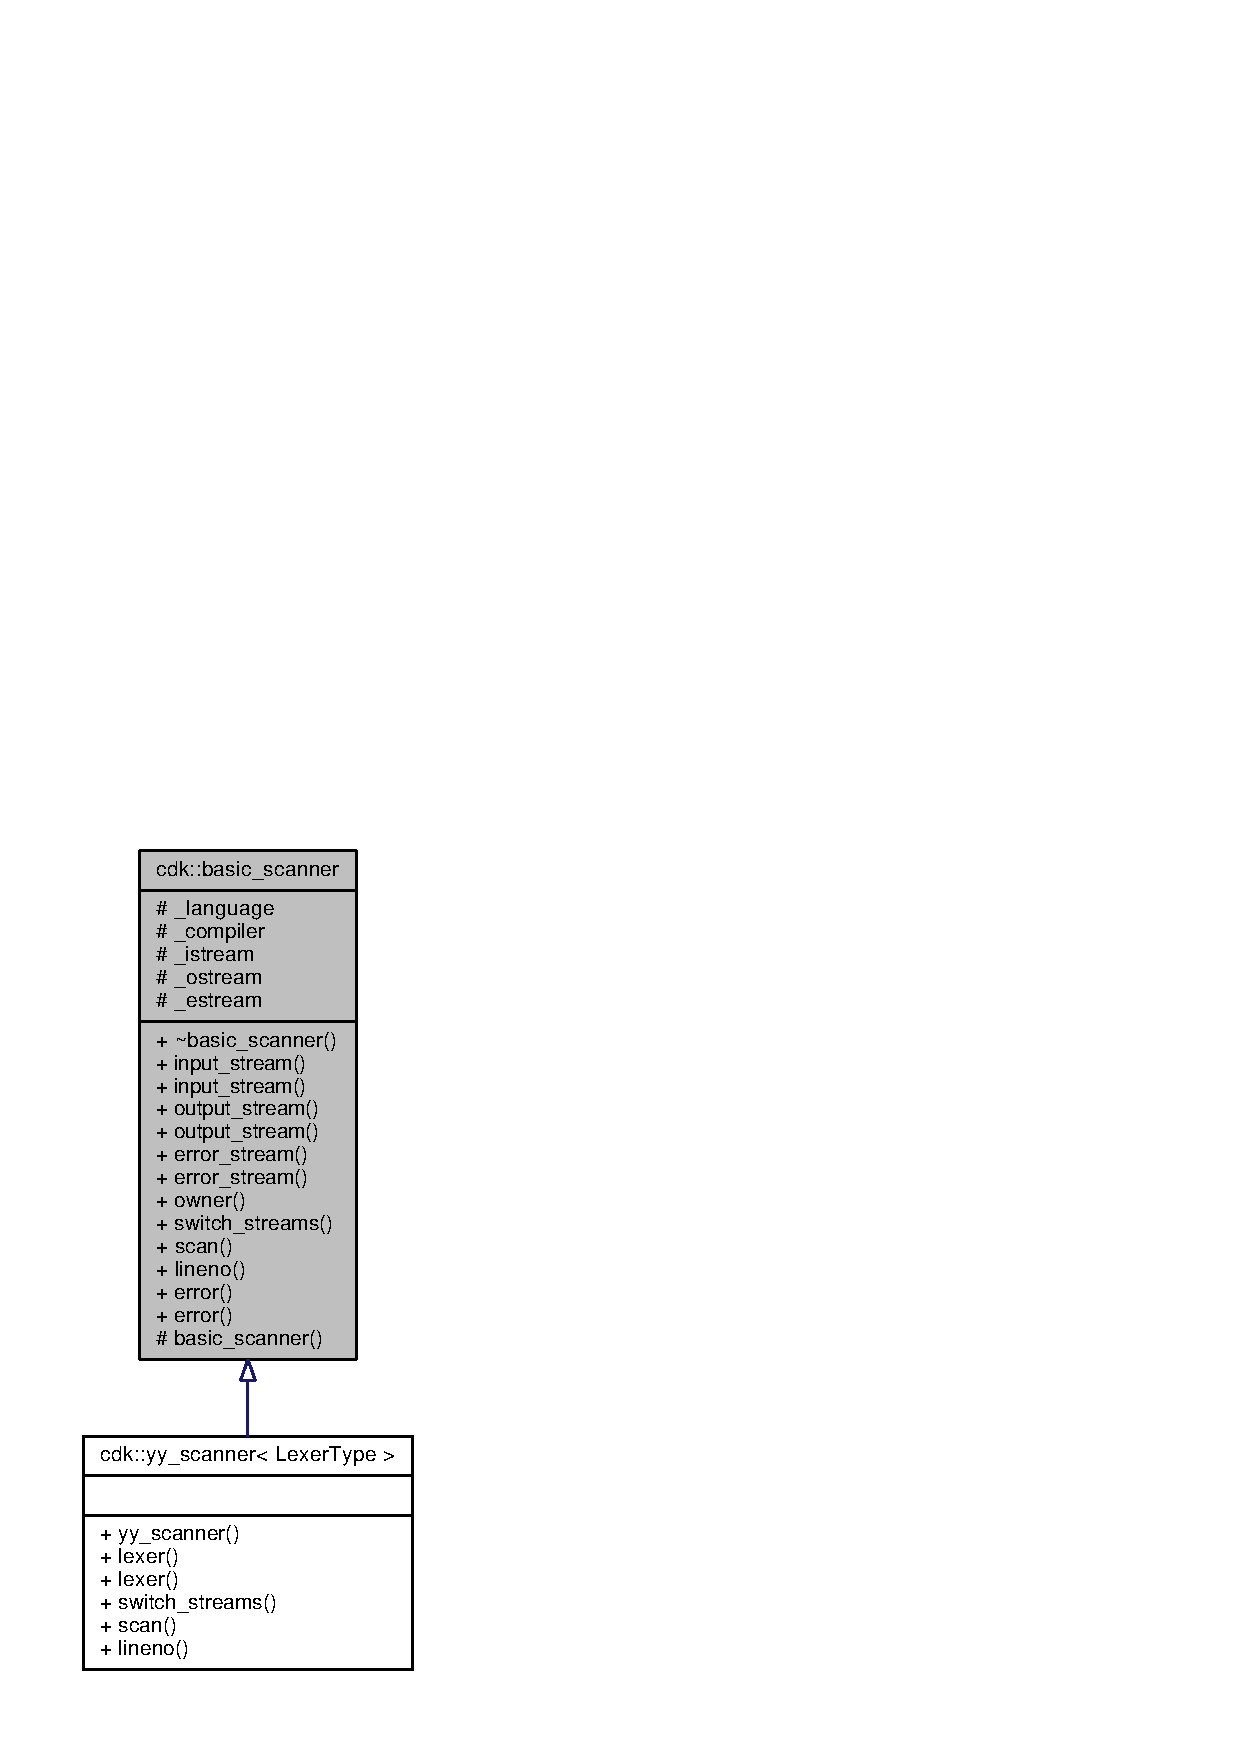
\includegraphics[width=202pt]{classcdk_1_1basic__scanner__inherit__graph}
\end{center}
\end{figure}


Collaboration diagram for cdk\+:\+:basic\+\_\+scanner\+:
\nopagebreak
\begin{figure}[H]
\begin{center}
\leavevmode
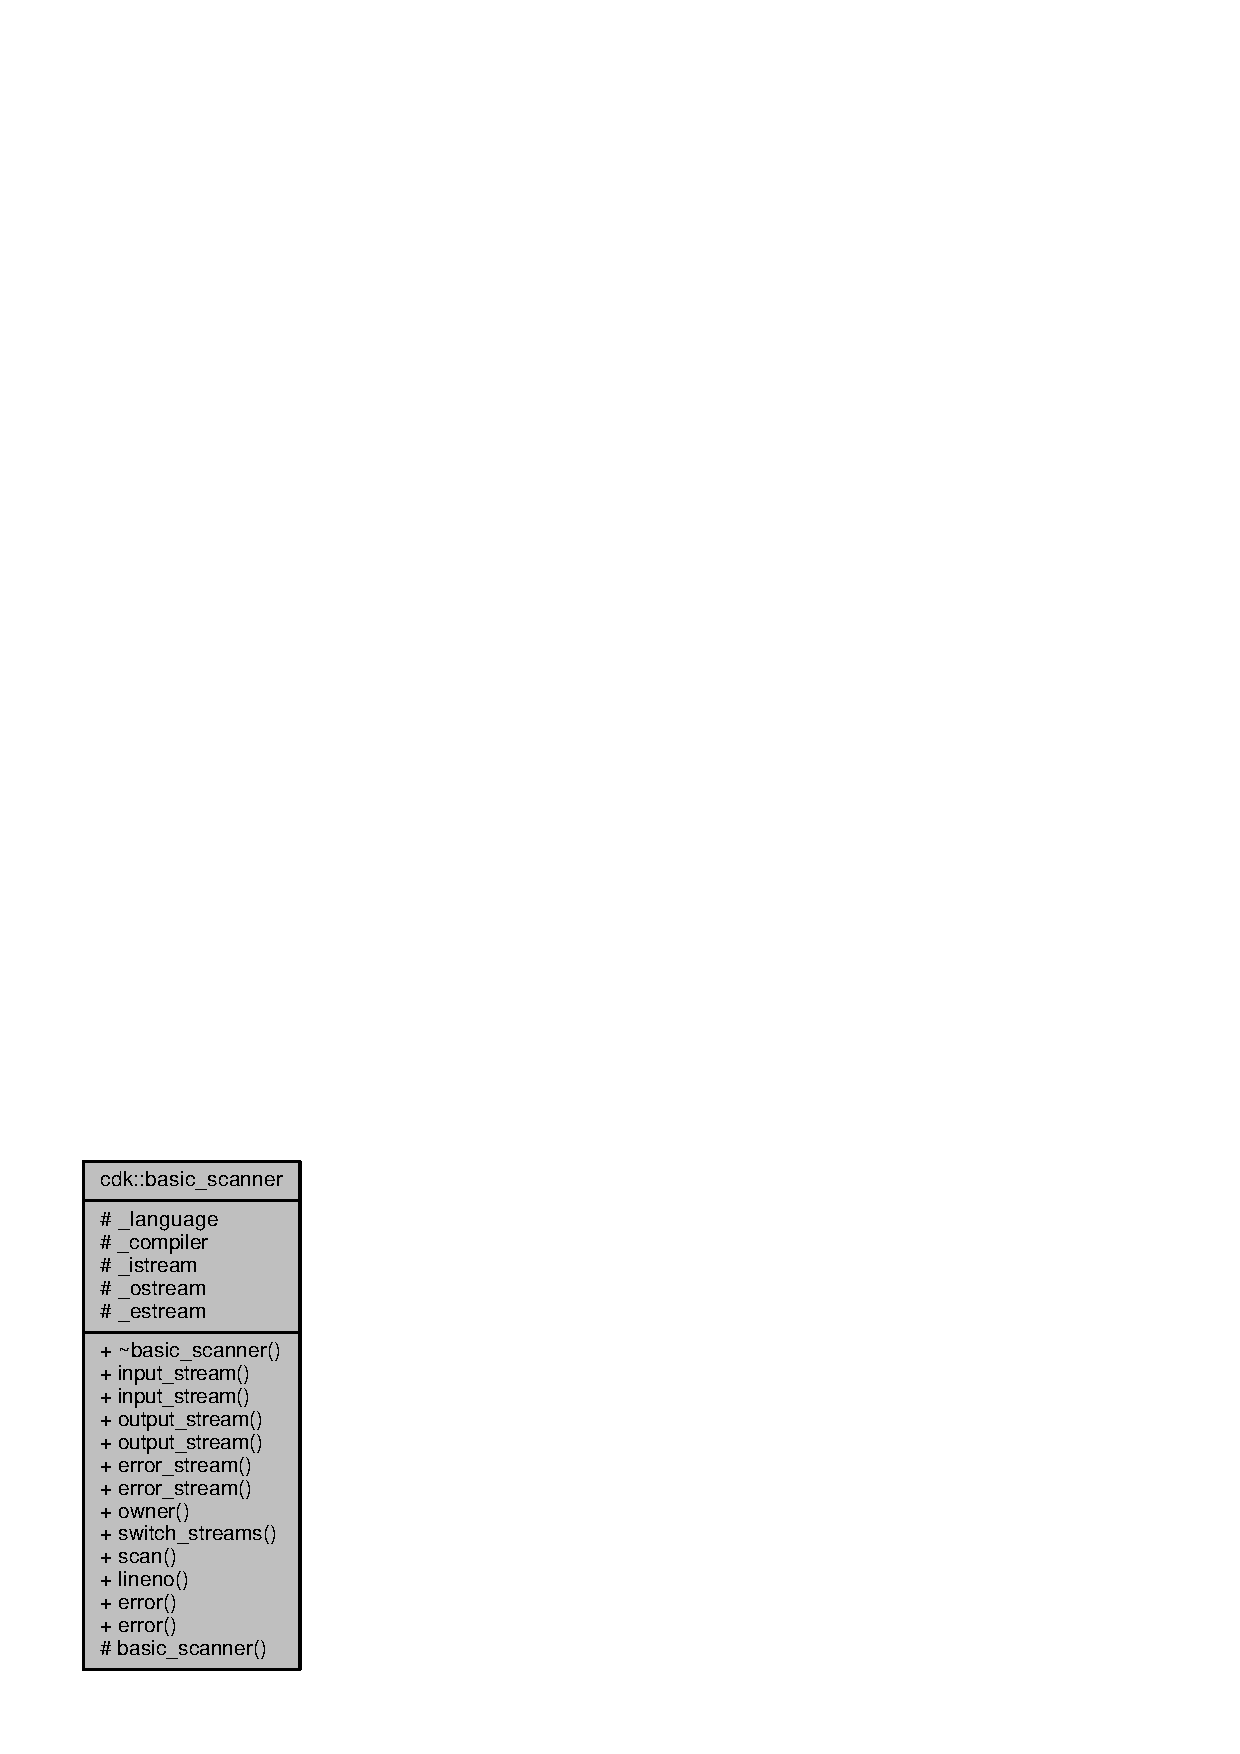
\includegraphics[width=148pt]{classcdk_1_1basic__scanner__coll__graph}
\end{center}
\end{figure}
\subsection*{Public Member Functions}
\begin{DoxyCompactItemize}
\item 
virtual {\bf $\sim$basic\+\_\+scanner} ()\label{classcdk_1_1basic__scanner_a84724c88be29e36456e3d91a4e6408e9}

\begin{DoxyCompactList}\small\item\em How to destroy a scanner. \end{DoxyCompactList}\item 
std\+::shared\+\_\+ptr$<$ std\+::istream $>$ {\bfseries input\+\_\+stream} ()\label{classcdk_1_1basic__scanner_a1844bebafdea3dddd4533e37c9c493f0}

\item 
void {\bfseries input\+\_\+stream} (std\+::shared\+\_\+ptr$<$ std\+::istream $>$ istr)\label{classcdk_1_1basic__scanner_a9c6dd4e6d2d776e670cde1c5801cb8c4}

\item 
std\+::shared\+\_\+ptr$<$ std\+::ostream $>$ {\bfseries output\+\_\+stream} ()\label{classcdk_1_1basic__scanner_a90349782202ffa3c4afd0368215d5c74}

\item 
void {\bfseries output\+\_\+stream} (std\+::shared\+\_\+ptr$<$ std\+::ostream $>$ ostr)\label{classcdk_1_1basic__scanner_af48b0fdaef91f8620fd8307a7bcce21f}

\item 
std\+::shared\+\_\+ptr$<$ std\+::ostream $>$ {\bfseries error\+\_\+stream} ()\label{classcdk_1_1basic__scanner_a7b915ebc3e30a39b98358fa0ab9e291e}

\item 
void {\bfseries error\+\_\+stream} (std\+::shared\+\_\+ptr$<$ std\+::ostream $>$ estr)\label{classcdk_1_1basic__scanner_a1907b7d54ba7b569a46abe427ef3c72e}

\item 
std\+::shared\+\_\+ptr$<$ {\bf compiler} $>$ {\bfseries owner} ()\label{classcdk_1_1basic__scanner_a5997574b9ef358ae140995d2b455146a}

\item 
virtual void {\bfseries switch\+\_\+streams} ()=0\label{classcdk_1_1basic__scanner_a945cd1fe3044cd563a21b5821f607a4e}

\item 
virtual int {\bf scan} ()=0
\item 
virtual int {\bf lineno} () const =0
\item 
virtual void {\bf error} (const std\+::string \&message) const 
\item 
virtual void {\bf error} (const char $\ast$const message) const 
\end{DoxyCompactItemize}
\subsection*{Protected Member Functions}
\begin{DoxyCompactItemize}
\item 
{\bfseries basic\+\_\+scanner} (const std\+::string \&language)\label{classcdk_1_1basic__scanner_a2248aa3bdf1cbbd99791c082c0ff0622}

\end{DoxyCompactItemize}
\subsection*{Protected Attributes}
\begin{DoxyCompactItemize}
\item 
const std\+::string {\bfseries \+\_\+language} = \char`\"{}\char`\"{}\label{classcdk_1_1basic__scanner_a5df3f99fae0e4d32f37a7c866b5a49f9}

\item 
std\+::shared\+\_\+ptr$<$ {\bf compiler} $>$ {\bfseries \+\_\+compiler} = nullptr\label{classcdk_1_1basic__scanner_adacdfd18dfe6318bbcf10d164e491a90}

\item 
std\+::shared\+\_\+ptr$<$ std\+::istream $>$ {\bfseries \+\_\+istream}
\item 
std\+::shared\+\_\+ptr$<$ std\+::ostream $>$ {\bfseries \+\_\+ostream}
\item 
std\+::shared\+\_\+ptr$<$ std\+::ostream $>$ {\bfseries \+\_\+estream}
\end{DoxyCompactItemize}
\subsection*{Friends}
\begin{DoxyCompactItemize}
\item 
class {\bfseries basic\+\_\+parser}\label{classcdk_1_1basic__scanner_a0cda9b397092fcd36f20439c161a8f79}

\item 
class {\bfseries compiler}\label{classcdk_1_1basic__scanner_a6450bc9182feebc4fe52fbf86fa0ba40}

\end{DoxyCompactItemize}


\subsection{Detailed Description}


Definition at line 15 of file basic\+\_\+scanner.\+h.



\subsection{Member Function Documentation}
\index{cdk\+::basic\+\_\+scanner@{cdk\+::basic\+\_\+scanner}!error@{error}}
\index{error@{error}!cdk\+::basic\+\_\+scanner@{cdk\+::basic\+\_\+scanner}}
\subsubsection[{error}]{\setlength{\rightskip}{0pt plus 5cm}virtual void cdk\+::basic\+\_\+scanner\+::error (
\begin{DoxyParamCaption}
\item[{const std\+::string \&}]{message}
\end{DoxyParamCaption}
) const\hspace{0.3cm}{\ttfamily [inline]}, {\ttfamily [virtual]}}\label{classcdk_1_1basic__scanner_a50d22c9986f6559e20b18522e0eae8d6}
Output error message. 

Definition at line 110 of file basic\+\_\+scanner.\+h.



References lineno().



Here is the call graph for this function\+:
\nopagebreak
\begin{figure}[H]
\begin{center}
\leavevmode
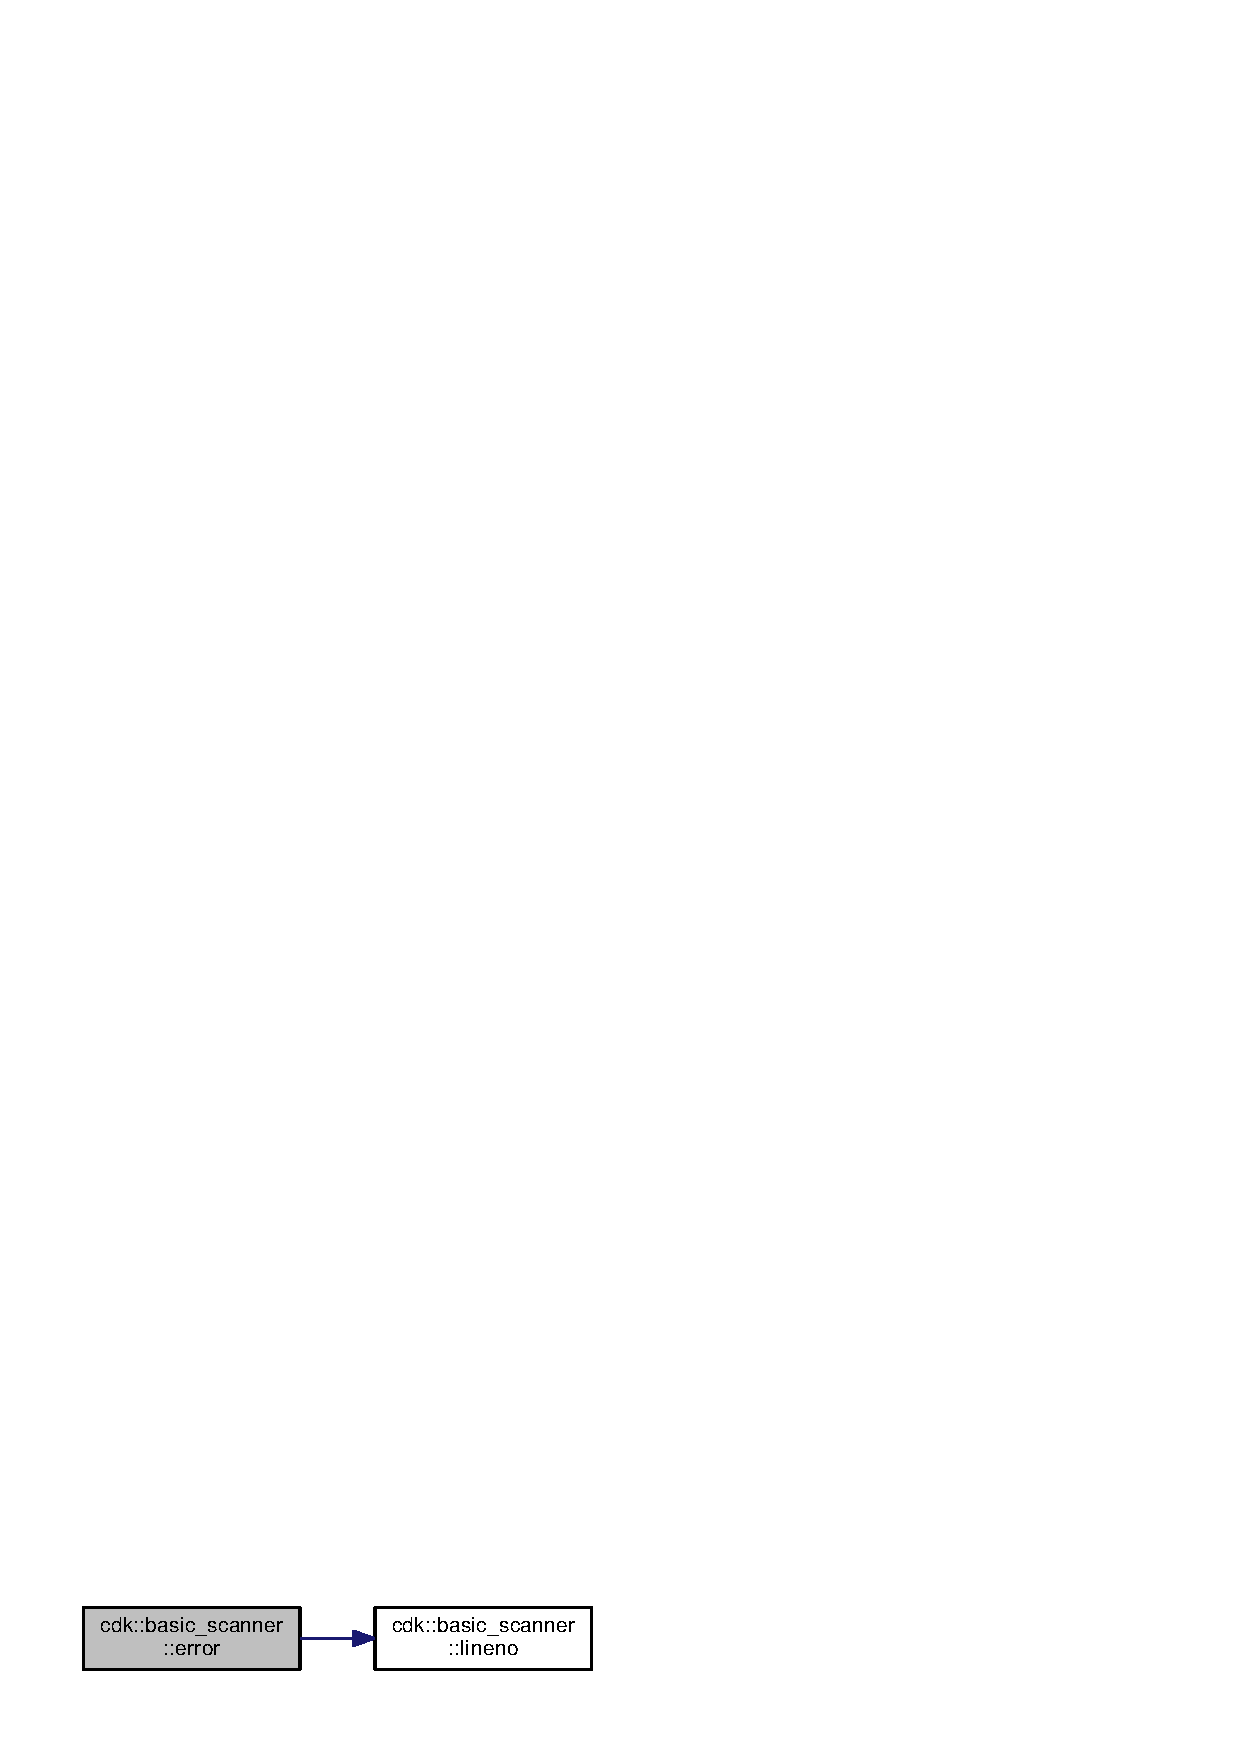
\includegraphics[width=288pt]{classcdk_1_1basic__scanner_a50d22c9986f6559e20b18522e0eae8d6_cgraph}
\end{center}
\end{figure}


\index{cdk\+::basic\+\_\+scanner@{cdk\+::basic\+\_\+scanner}!error@{error}}
\index{error@{error}!cdk\+::basic\+\_\+scanner@{cdk\+::basic\+\_\+scanner}}
\subsubsection[{error}]{\setlength{\rightskip}{0pt plus 5cm}virtual void cdk\+::basic\+\_\+scanner\+::error (
\begin{DoxyParamCaption}
\item[{const char $\ast$const}]{message}
\end{DoxyParamCaption}
) const\hspace{0.3cm}{\ttfamily [inline]}, {\ttfamily [virtual]}}\label{classcdk_1_1basic__scanner_a3ba3fc8471abf2d50b9a86c97a66a2ed}
Output error message. 

Definition at line 117 of file basic\+\_\+scanner.\+h.



References lineno().



Here is the call graph for this function\+:
\nopagebreak
\begin{figure}[H]
\begin{center}
\leavevmode
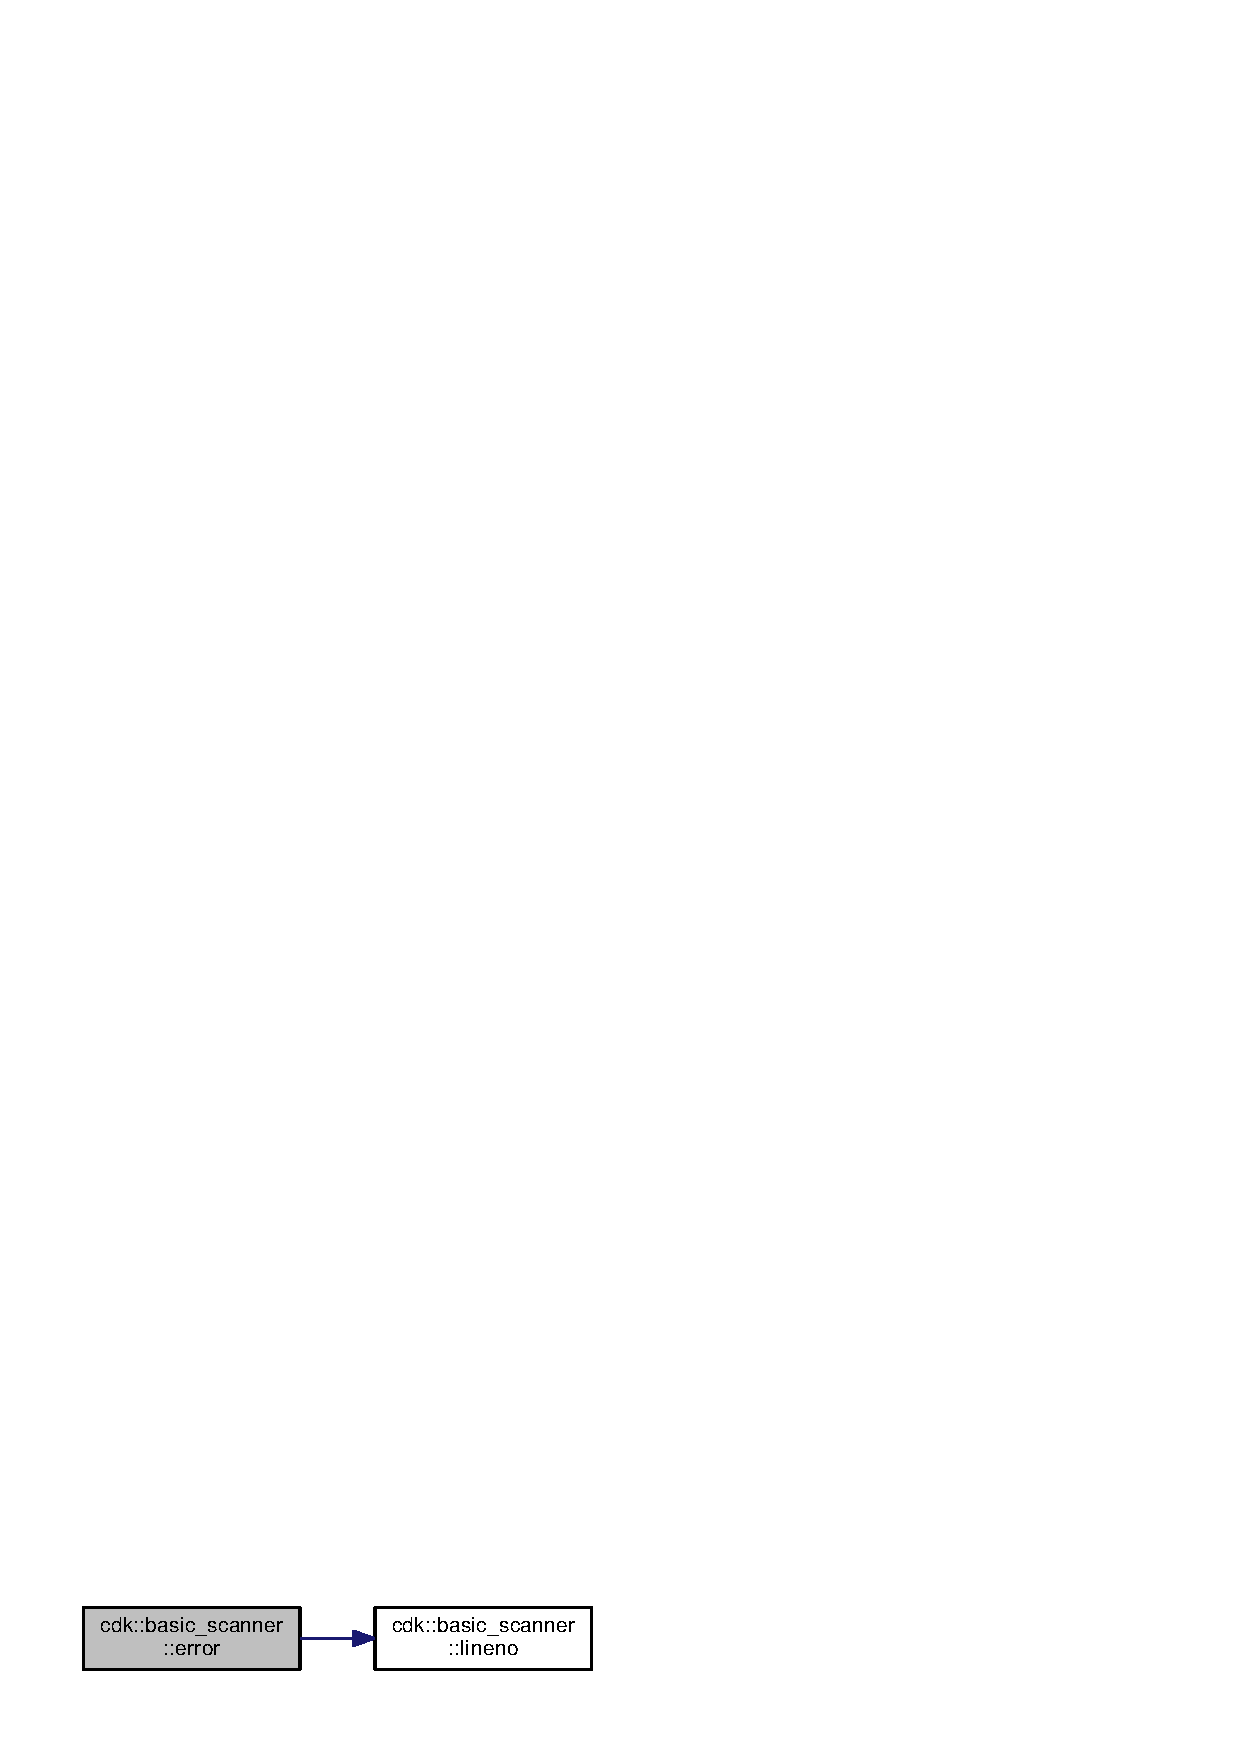
\includegraphics[width=288pt]{classcdk_1_1basic__scanner_a3ba3fc8471abf2d50b9a86c97a66a2ed_cgraph}
\end{center}
\end{figure}


\index{cdk\+::basic\+\_\+scanner@{cdk\+::basic\+\_\+scanner}!lineno@{lineno}}
\index{lineno@{lineno}!cdk\+::basic\+\_\+scanner@{cdk\+::basic\+\_\+scanner}}
\subsubsection[{lineno}]{\setlength{\rightskip}{0pt plus 5cm}virtual int cdk\+::basic\+\_\+scanner\+::lineno (
\begin{DoxyParamCaption}
{}
\end{DoxyParamCaption}
) const\hspace{0.3cm}{\ttfamily [pure virtual]}}\label{classcdk_1_1basic__scanner_a958d6207e97b29606410fba4204a60db}
Return current source line. 

Implemented in {\bf cdk\+::yy\+\_\+scanner$<$ Lexer\+Type $>$} \doxyref{}{p.}{classcdk_1_1yy__scanner_a5a4af647608bcfbcb1c022c75b6ce093}.



Referenced by error().

\index{cdk\+::basic\+\_\+scanner@{cdk\+::basic\+\_\+scanner}!scan@{scan}}
\index{scan@{scan}!cdk\+::basic\+\_\+scanner@{cdk\+::basic\+\_\+scanner}}
\subsubsection[{scan}]{\setlength{\rightskip}{0pt plus 5cm}virtual int cdk\+::basic\+\_\+scanner\+::scan (
\begin{DoxyParamCaption}
{}
\end{DoxyParamCaption}
)\hspace{0.3cm}{\ttfamily [pure virtual]}}\label{classcdk_1_1basic__scanner_aad8bc66ab0e2247392a91057b1bd55cf}
Scanning algorithm\+: the compiler object stores the result. 
\begin{DoxyParams}{Parameters}
{\em compiler} & the compiler object this parser belongs to. \\
\hline
\end{DoxyParams}
\begin{DoxyReturn}{Returns}
true if the operation is successful 
\end{DoxyReturn}


Implemented in {\bf cdk\+::yy\+\_\+scanner$<$ Lexer\+Type $>$} \doxyref{}{p.}{classcdk_1_1yy__scanner_af3a3f2fc181718ef27ea44870474e3ec}.



\subsection{Member Data Documentation}
\index{cdk\+::basic\+\_\+scanner@{cdk\+::basic\+\_\+scanner}!\+\_\+estream@{\+\_\+estream}}
\index{\+\_\+estream@{\+\_\+estream}!cdk\+::basic\+\_\+scanner@{cdk\+::basic\+\_\+scanner}}
\subsubsection[{\+\_\+estream}]{\setlength{\rightskip}{0pt plus 5cm}std\+::shared\+\_\+ptr$<$std\+::ostream$>$ cdk\+::basic\+\_\+scanner\+::\+\_\+estream\hspace{0.3cm}{\ttfamily [protected]}}\label{classcdk_1_1basic__scanner_ac0c7edce1f9288b2cc5a93087807879c}
{\bfseries Initial value\+:}
\begin{DoxyCode}
= std::shared\_ptr<std::ostream>(&std::cerr,
                                                                           null\_deleter())
\end{DoxyCode}


Definition at line 37 of file basic\+\_\+scanner.\+h.

\index{cdk\+::basic\+\_\+scanner@{cdk\+::basic\+\_\+scanner}!\+\_\+istream@{\+\_\+istream}}
\index{\+\_\+istream@{\+\_\+istream}!cdk\+::basic\+\_\+scanner@{cdk\+::basic\+\_\+scanner}}
\subsubsection[{\+\_\+istream}]{\setlength{\rightskip}{0pt plus 5cm}std\+::shared\+\_\+ptr$<$std\+::istream$>$ cdk\+::basic\+\_\+scanner\+::\+\_\+istream\hspace{0.3cm}{\ttfamily [protected]}}\label{classcdk_1_1basic__scanner_af1c1bc5c903b5335ad6d4ddd28ea1c65}
{\bfseries Initial value\+:}
\begin{DoxyCode}
= std::shared\_ptr<std::istream>(&std::cin,
                                                                           null\_deleter())
\end{DoxyCode}


Definition at line 29 of file basic\+\_\+scanner.\+h.

\index{cdk\+::basic\+\_\+scanner@{cdk\+::basic\+\_\+scanner}!\+\_\+ostream@{\+\_\+ostream}}
\index{\+\_\+ostream@{\+\_\+ostream}!cdk\+::basic\+\_\+scanner@{cdk\+::basic\+\_\+scanner}}
\subsubsection[{\+\_\+ostream}]{\setlength{\rightskip}{0pt plus 5cm}std\+::shared\+\_\+ptr$<$std\+::ostream$>$ cdk\+::basic\+\_\+scanner\+::\+\_\+ostream\hspace{0.3cm}{\ttfamily [protected]}}\label{classcdk_1_1basic__scanner_a4a1e22ea48e5cbe116e68f99b7463096}
{\bfseries Initial value\+:}
\begin{DoxyCode}
= std::shared\_ptr<std::ostream>(&std::cout,
                                                                           null\_deleter())
\end{DoxyCode}


Definition at line 33 of file basic\+\_\+scanner.\+h.



The documentation for this class was generated from the following file\+:\begin{DoxyCompactItemize}
\item 
basic\+\_\+scanner.\+h\end{DoxyCompactItemize}

\section{cdk\+:\+:basic\+\_\+target Class Reference}
\label{classcdk_1_1basic__target}\index{cdk\+::basic\+\_\+target@{cdk\+::basic\+\_\+target}}


Collaboration diagram for cdk\+:\+:basic\+\_\+target\+:
\nopagebreak
\begin{figure}[H]
\begin{center}
\leavevmode
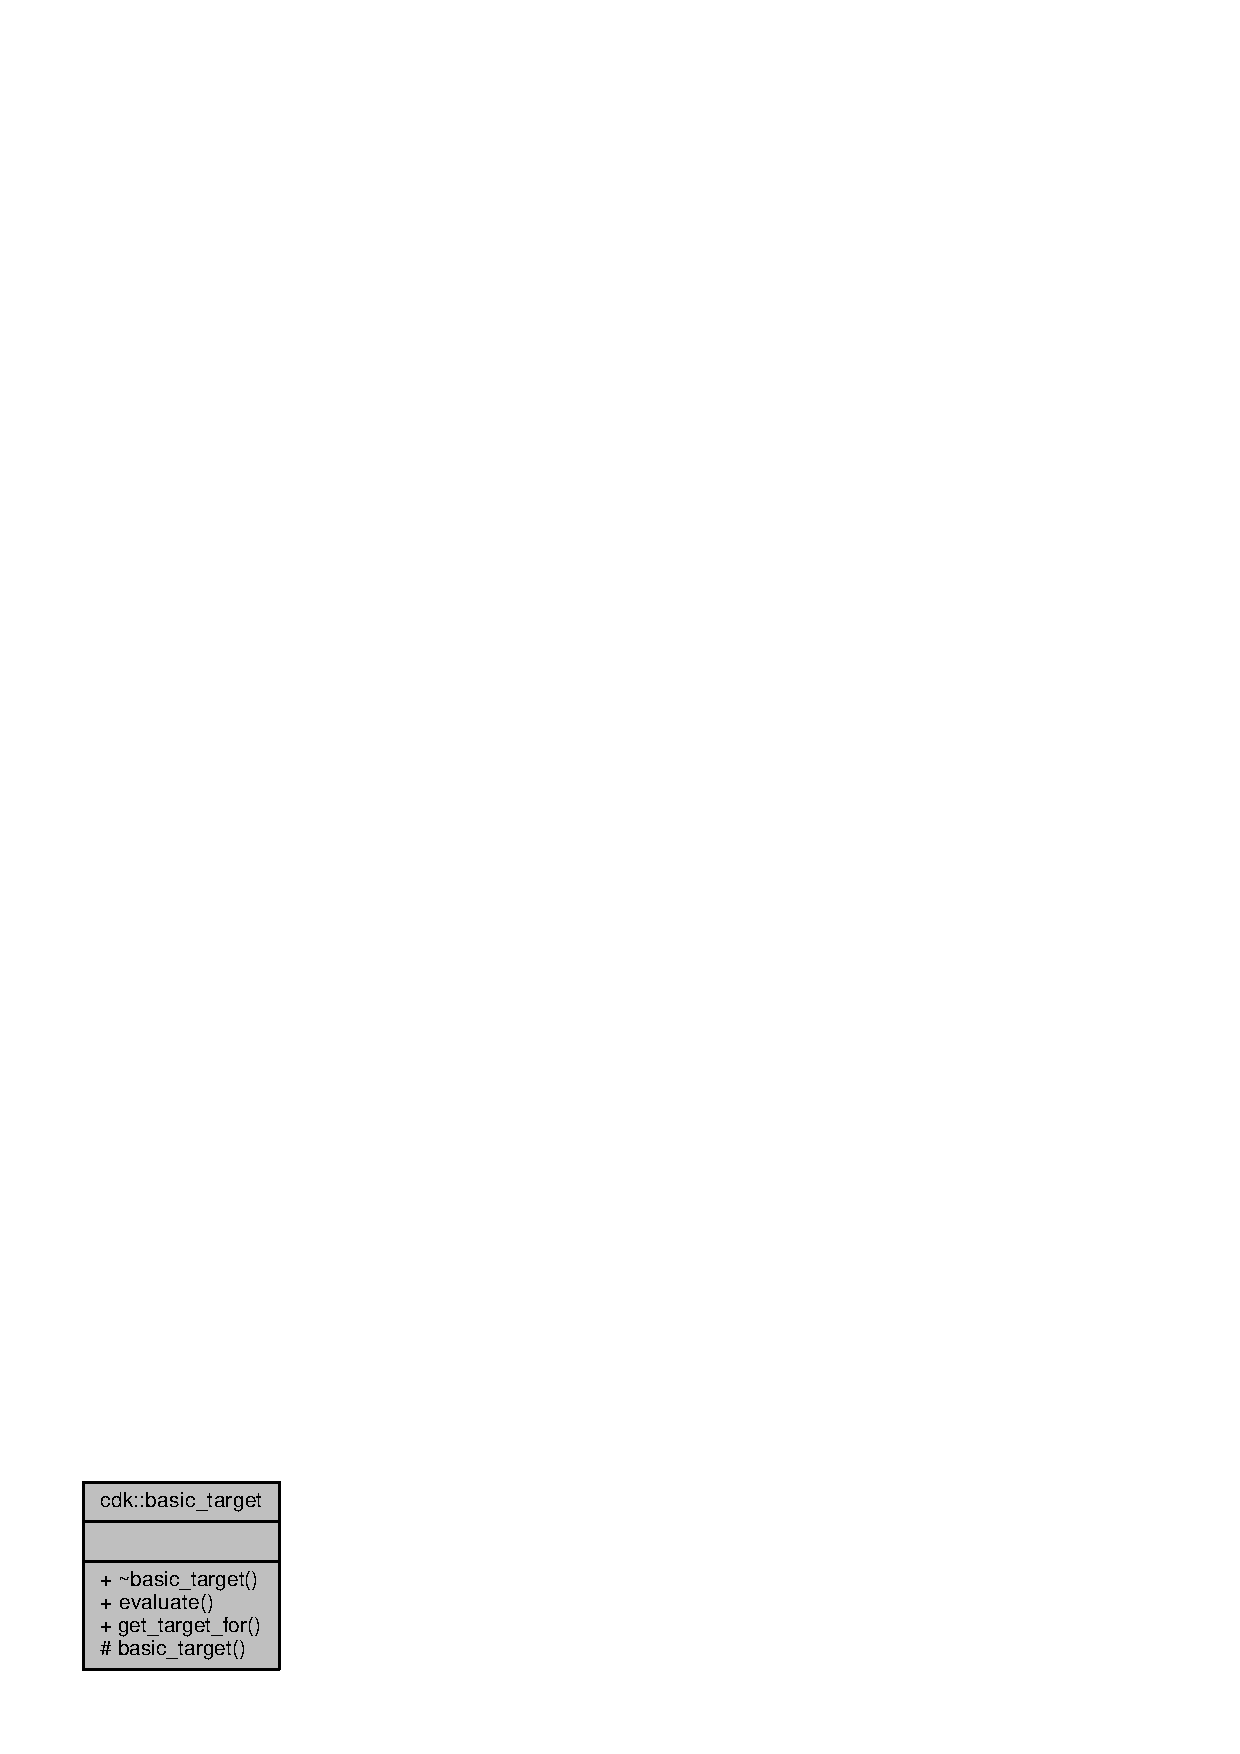
\includegraphics[width=138pt]{classcdk_1_1basic__target__coll__graph}
\end{center}
\end{figure}
\subsection*{Public Member Functions}
\begin{DoxyCompactItemize}
\item 
virtual {\bf $\sim$basic\+\_\+target} ()\label{classcdk_1_1basic__target_aaa74cb39cf10b2735b1abc15680898fa}

\begin{DoxyCompactList}\small\item\em How to destroy an evaluator. \end{DoxyCompactList}\item 
virtual bool {\bf evaluate} (std\+::shared\+\_\+ptr$<$ {\bf compiler} $>$)=0
\end{DoxyCompactItemize}
\subsection*{Static Public Member Functions}
\begin{DoxyCompactItemize}
\item 
static {\bf basic\+\_\+target} $\ast$ {\bf get\+\_\+target\+\_\+for} (const std\+::string \&target)
\end{DoxyCompactItemize}
\subsection*{Protected Member Functions}
\begin{DoxyCompactItemize}
\item 
{\bfseries basic\+\_\+target} (const char $\ast$target)\label{classcdk_1_1basic__target_a789431eed534e3827eb2686ed00f30b8}

\end{DoxyCompactItemize}


\subsection{Detailed Description}


Definition at line 16 of file basic\+\_\+target.\+h.



\subsection{Member Function Documentation}
\index{cdk\+::basic\+\_\+target@{cdk\+::basic\+\_\+target}!evaluate@{evaluate}}
\index{evaluate@{evaluate}!cdk\+::basic\+\_\+target@{cdk\+::basic\+\_\+target}}
\subsubsection[{evaluate}]{\setlength{\rightskip}{0pt plus 5cm}virtual bool cdk\+::basic\+\_\+target\+::evaluate (
\begin{DoxyParamCaption}
\item[{std\+::shared\+\_\+ptr$<$ {\bf compiler} $>$}]{}
\end{DoxyParamCaption}
)\hspace{0.3cm}{\ttfamily [pure virtual]}}\label{classcdk_1_1basic__target_a0db773c9c4f84a36df0949187aab9adb}
Evaluation algorithm for a syntax tree\+: processes the tree and sends the result to the output stream. 
\begin{DoxyParams}{Parameters}
{\em compiler} & object representing the compiler as a whole \\
\hline
\end{DoxyParams}
\begin{DoxyReturn}{Returns}
true if the operation is successful 
\end{DoxyReturn}


Referenced by cdk\+::compiler\+::evaluate().

\index{cdk\+::basic\+\_\+target@{cdk\+::basic\+\_\+target}!get\+\_\+target\+\_\+for@{get\+\_\+target\+\_\+for}}
\index{get\+\_\+target\+\_\+for@{get\+\_\+target\+\_\+for}!cdk\+::basic\+\_\+target@{cdk\+::basic\+\_\+target}}
\subsubsection[{get\+\_\+target\+\_\+for}]{\setlength{\rightskip}{0pt plus 5cm}static {\bf basic\+\_\+target}$\ast$ cdk\+::basic\+\_\+target\+::get\+\_\+target\+\_\+for (
\begin{DoxyParamCaption}
\item[{const std\+::string \&}]{target}
\end{DoxyParamCaption}
)\hspace{0.3cm}{\ttfamily [inline]}, {\ttfamily [static]}}\label{classcdk_1_1basic__target_a50126c8601a5b82dcce46e43d4258064}
How to get an evaluator for a given target. 
\begin{DoxyParams}{Parameters}
{\em target} & the target name\+: \char`\"{}asm\char`\"{}, \char`\"{}c\char`\"{}, \char`\"{}xml\char`\"{}, etc. \\
\hline
\end{DoxyParams}
\begin{DoxyReturn}{Returns}
a pointer to the evaluator object 
\end{DoxyReturn}


Definition at line 33 of file basic\+\_\+target.\+h.



Referenced by cdk\+::compiler\+::evaluate().



The documentation for this class was generated from the following file\+:\begin{DoxyCompactItemize}
\item 
basic\+\_\+target.\+h\end{DoxyCompactItemize}

\section{basic\+\_\+type Struct Reference}
\label{structbasic__type}\index{basic\+\_\+type@{basic\+\_\+type}}


{\ttfamily \#include $<$basic\+\_\+type.\+h$>$}



Collaboration diagram for basic\+\_\+type\+:
\nopagebreak
\begin{figure}[H]
\begin{center}
\leavevmode
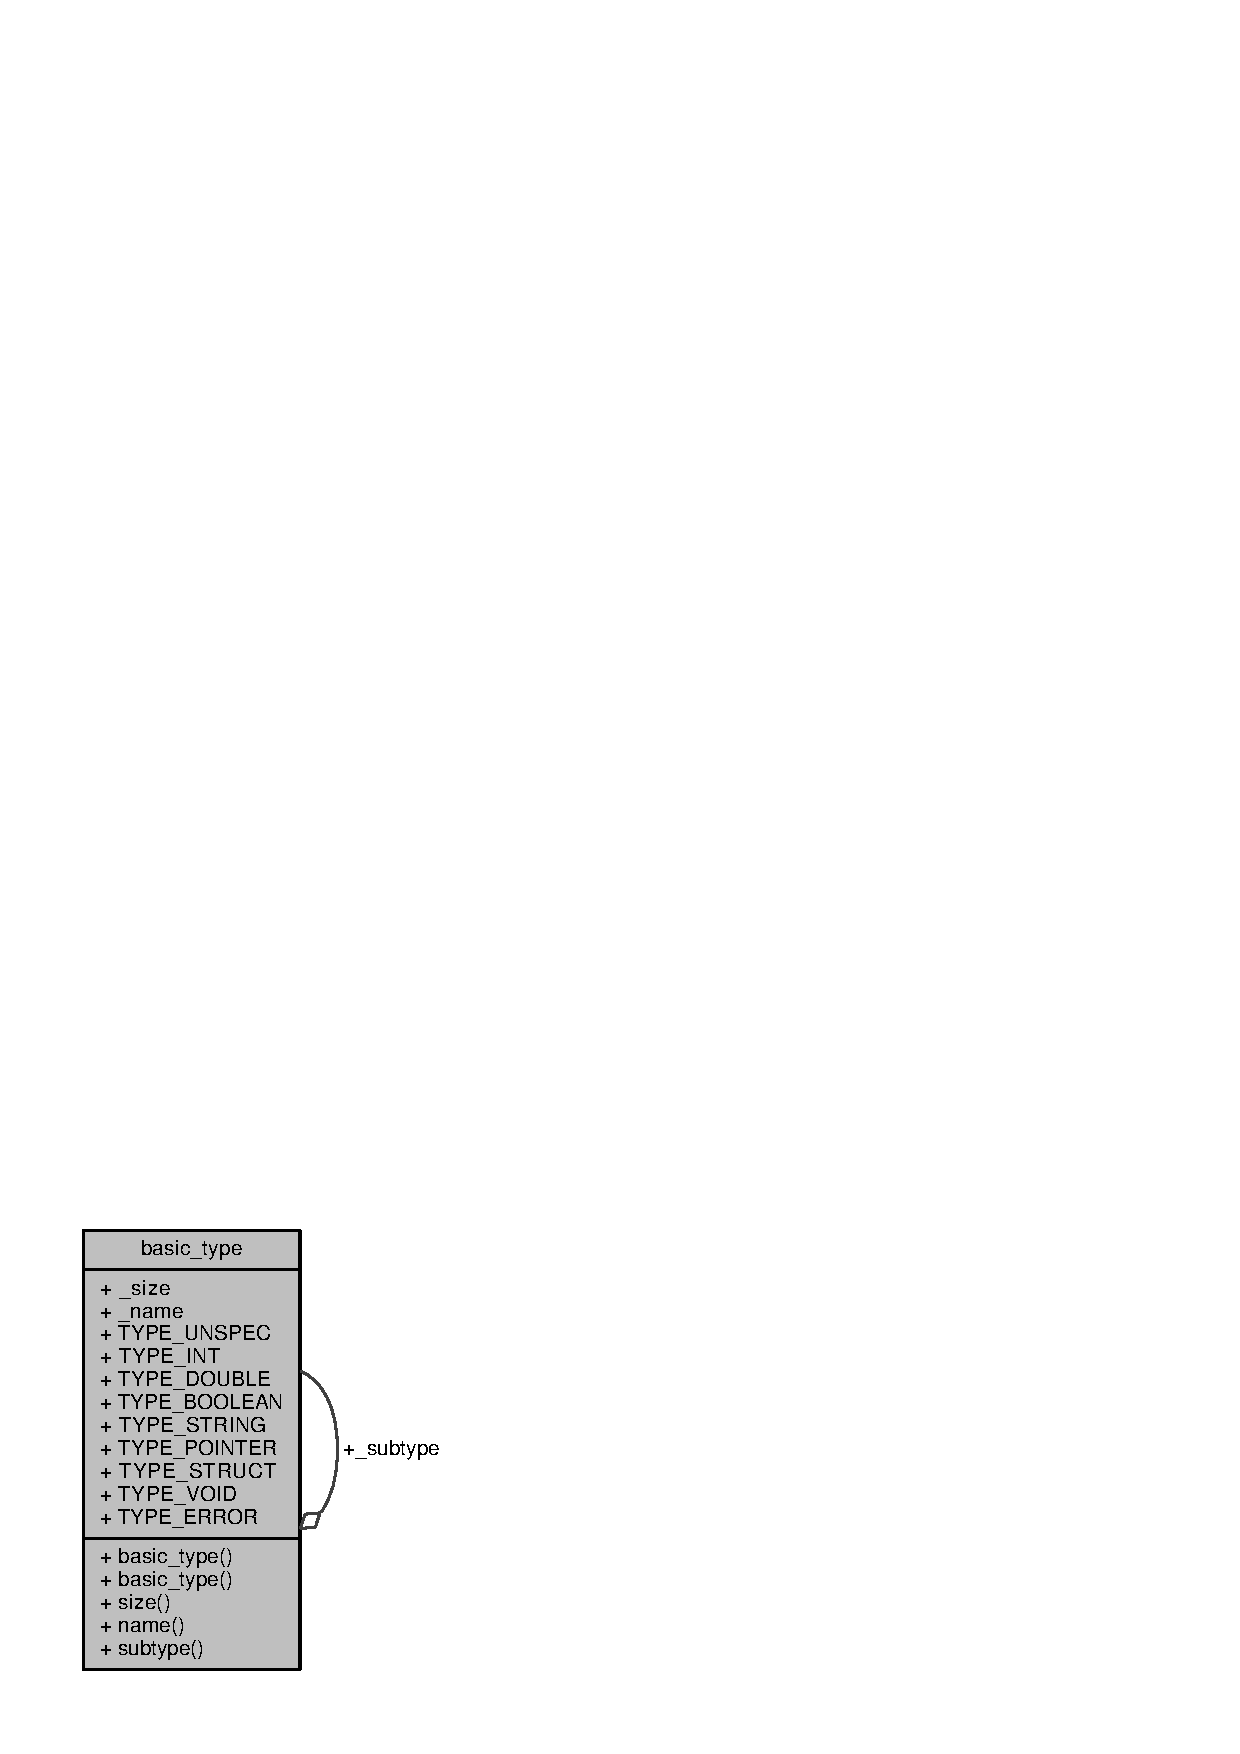
\includegraphics[width=215pt]{structbasic__type__coll__graph}
\end{center}
\end{figure}
\subsection*{Public Types}
\begin{DoxyCompactItemize}
\item 
typedef unsigned long int {\bfseries type}\label{structbasic__type_a7c0a7a590da8a3705a88d5e207e4b9ad}

\end{DoxyCompactItemize}
\subsection*{Public Member Functions}
\begin{DoxyCompactItemize}
\item 
{\bfseries basic\+\_\+type} (size\+\_\+t size, type name)\label{structbasic__type_a700988000343593c00601ec255b04d0b}

\item 
size\+\_\+t {\bfseries size} ()\label{structbasic__type_a4f76b416ac41dde6d7a9f51d7e909891}

\item 
type {\bfseries name} ()\label{structbasic__type_aaf747bec5153a84f07097482a77eae29}

\item 
{\bf basic\+\_\+type} $\ast$ {\bfseries subtype} ()\label{structbasic__type_ac3c708c8bbd2274461227daee6b50a6a}

\end{DoxyCompactItemize}
\subsection*{Public Attributes}
\begin{DoxyCompactItemize}
\item 
size\+\_\+t {\bfseries \+\_\+size} = 0\label{structbasic__type_a7d0e7cd683e46caea2c165fb8ebf26c5}

\item 
type {\bfseries \+\_\+name} = T\+Y\+P\+E\+\_\+\+U\+N\+S\+P\+E\+C\label{structbasic__type_a3fc97d3a8fc1f7ab3d037359ad705a42}

\item 
{\bf basic\+\_\+type} $\ast$ {\bfseries \+\_\+subtype} = nullptr\label{structbasic__type_a2ce9b0a06193a2bd685f106bc72a6089}

\end{DoxyCompactItemize}
\subsection*{Static Public Attributes}
\begin{DoxyCompactItemize}
\item 
static const type {\bfseries T\+Y\+P\+E\+\_\+\+U\+N\+S\+P\+E\+C} = 0\label{structbasic__type_a7787995e345f10d3cc6c48d0708c8a36}

\item 
static const type {\bfseries T\+Y\+P\+E\+\_\+\+I\+N\+T} = 1\+U\+L$<$$<$0\label{structbasic__type_a6c904b5d042062de5ac5c454bc9426a6}

\item 
static const type {\bfseries T\+Y\+P\+E\+\_\+\+D\+O\+U\+B\+L\+E} = 1\+U\+L$<$$<$1\label{structbasic__type_aa8786b1860b50978829feb20e614b4c3}

\item 
static const type {\bfseries T\+Y\+P\+E\+\_\+\+B\+O\+O\+L\+E\+A\+N} = 1\+U\+L$<$$<$2\label{structbasic__type_a62f257e76816cc338762e6a1182174ef}

\item 
static const type {\bfseries T\+Y\+P\+E\+\_\+\+S\+T\+R\+I\+N\+G} = 1\+U\+L$<$$<$3\label{structbasic__type_a2f6ab0d223597c328005e6c2276f523e}

\item 
static const type {\bfseries T\+Y\+P\+E\+\_\+\+P\+O\+I\+N\+T\+E\+R} = 1\+U\+L$<$$<$4\label{structbasic__type_a9ded574c7b6d0a63acd29b87d8c16efe}

\item 
static const type {\bfseries T\+Y\+P\+E\+\_\+\+S\+T\+R\+U\+C\+T} = 1\+U\+L$<$$<$5\label{structbasic__type_a0e3320ba9749776fbf1303d353fec55e}

\item 
static const type {\bfseries T\+Y\+P\+E\+\_\+\+V\+O\+I\+D} = 1\+U\+L$<$$<$30\label{structbasic__type_a59e3a52115cbe7ac8a43d64072bb98a3}

\item 
static const type {\bfseries T\+Y\+P\+E\+\_\+\+E\+R\+R\+O\+R} = 1\+U\+L$<$$<$31\label{structbasic__type_af5146fc165cffff72de991842d60840c}

\end{DoxyCompactItemize}


\subsection{Detailed Description}
This is a quick and very dirty approach to type information. It is defined this way (even though it's not extensible at all) for simplicity.

Nevertheless, new types can be added simply by using other integer values other than the ones listed. 

Definition at line 15 of file basic\+\_\+type.\+h.



The documentation for this struct was generated from the following file\+:\begin{DoxyCompactItemize}
\item 
basic\+\_\+type.\+h\end{DoxyCompactItemize}

\section{cdk\+:\+:binary\+\_\+expression\+\_\+node Class Reference}
\label{classcdk_1_1binary__expression__node}\index{cdk\+::binary\+\_\+expression\+\_\+node@{cdk\+::binary\+\_\+expression\+\_\+node}}


{\ttfamily \#include $<$binary\+\_\+expression\+\_\+node.\+h$>$}



Inheritance diagram for cdk\+:\+:binary\+\_\+expression\+\_\+node\+:
\nopagebreak
\begin{figure}[H]
\begin{center}
\leavevmode
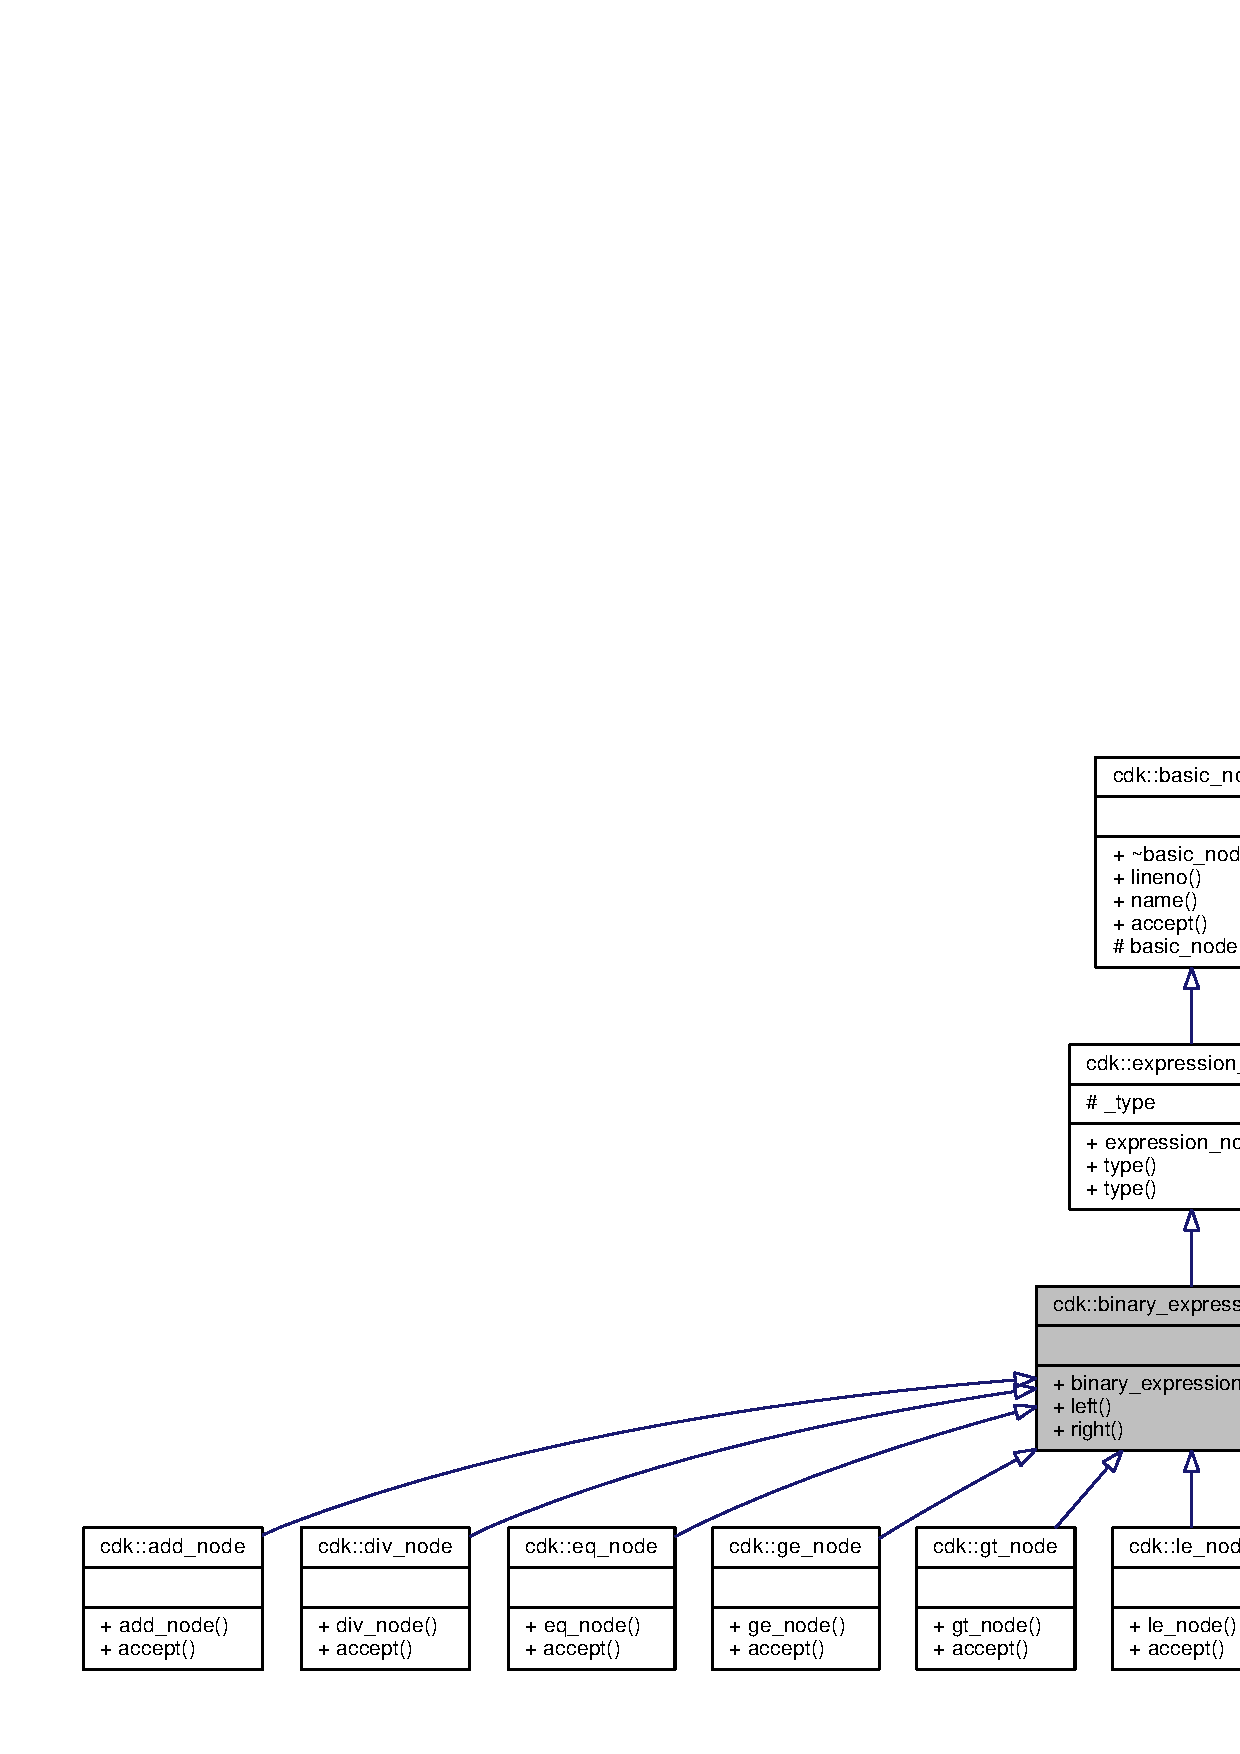
\includegraphics[width=350pt]{classcdk_1_1binary__expression__node__inherit__graph}
\end{center}
\end{figure}


Collaboration diagram for cdk\+:\+:binary\+\_\+expression\+\_\+node\+:
\nopagebreak
\begin{figure}[H]
\begin{center}
\leavevmode
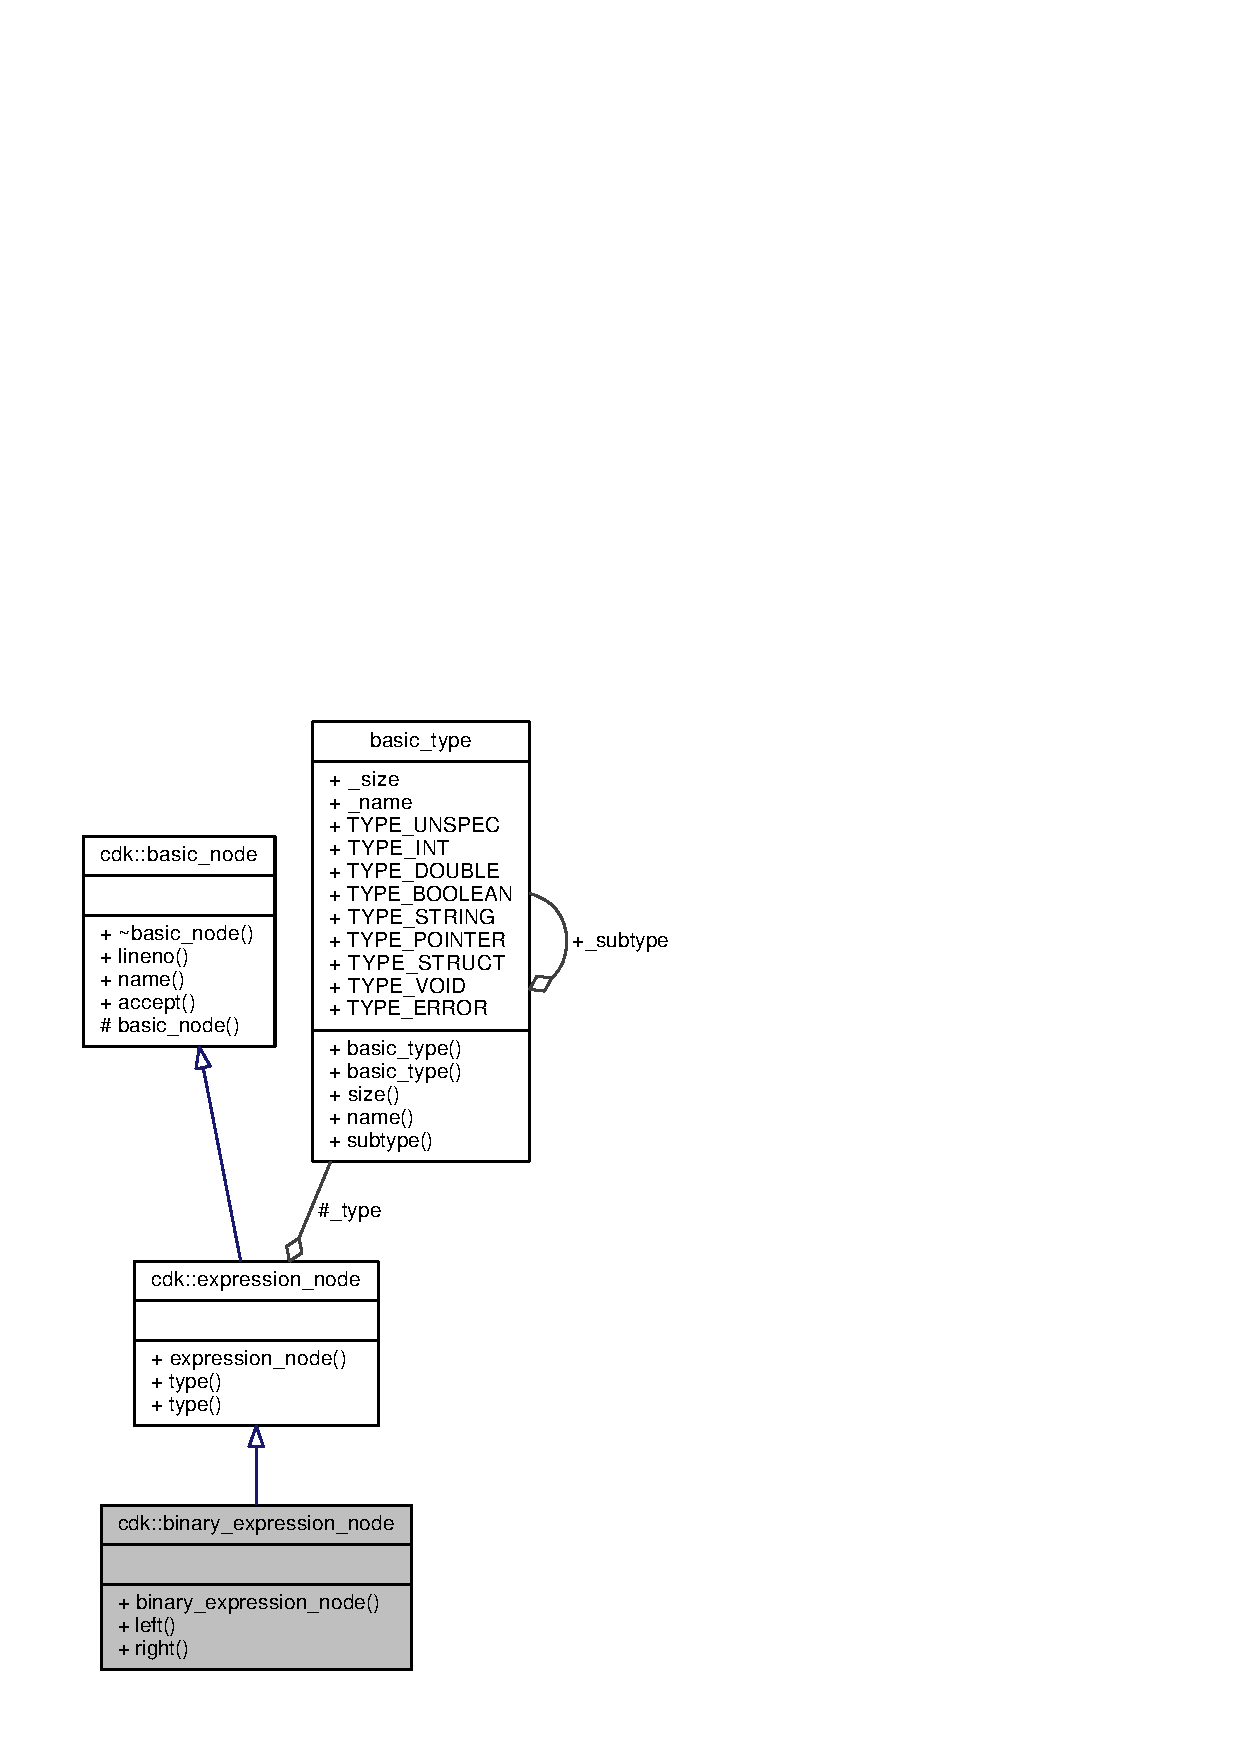
\includegraphics[width=325pt]{classcdk_1_1binary__expression__node__coll__graph}
\end{center}
\end{figure}
\subsection*{Public Member Functions}
\begin{DoxyCompactItemize}
\item 
{\bf binary\+\_\+expression\+\_\+node} (int {\bf lineno}, {\bf expression\+\_\+node} $\ast$left, {\bf expression\+\_\+node} $\ast$right)
\item 
{\bf expression\+\_\+node} $\ast$ {\bfseries left} ()\label{classcdk_1_1binary__expression__node_a8ac0b884a1ea56ed16d78997066d120d}

\item 
{\bf expression\+\_\+node} $\ast$ {\bfseries right} ()\label{classcdk_1_1binary__expression__node_a763e869d08583a828bd1b6b5433dde52}

\end{DoxyCompactItemize}
\subsection*{Additional Inherited Members}


\subsection{Detailed Description}
Class for describing binary operators. 

Definition at line 12 of file binary\+\_\+expression\+\_\+node.\+h.



\subsection{Constructor \& Destructor Documentation}
\index{cdk\+::binary\+\_\+expression\+\_\+node@{cdk\+::binary\+\_\+expression\+\_\+node}!binary\+\_\+expression\+\_\+node@{binary\+\_\+expression\+\_\+node}}
\index{binary\+\_\+expression\+\_\+node@{binary\+\_\+expression\+\_\+node}!cdk\+::binary\+\_\+expression\+\_\+node@{cdk\+::binary\+\_\+expression\+\_\+node}}
\subsubsection[{binary\+\_\+expression\+\_\+node}]{\setlength{\rightskip}{0pt plus 5cm}cdk\+::binary\+\_\+expression\+\_\+node\+::binary\+\_\+expression\+\_\+node (
\begin{DoxyParamCaption}
\item[{int}]{lineno, }
\item[{{\bf expression\+\_\+node} $\ast$}]{left, }
\item[{{\bf expression\+\_\+node} $\ast$}]{right}
\end{DoxyParamCaption}
)\hspace{0.3cm}{\ttfamily [inline]}}\label{classcdk_1_1binary__expression__node_a06fa367b484369bec4645ea5274b46df}

\begin{DoxyParams}{Parameters}
{\em lineno} & source code line number for this node \\
\hline
{\em left} & first operand \\
\hline
{\em right} & second operand \\
\hline
\end{DoxyParams}


Definition at line 21 of file binary\+\_\+expression\+\_\+node.\+h.



The documentation for this class was generated from the following file\+:\begin{DoxyCompactItemize}
\item 
ast/binary\+\_\+expression\+\_\+node.\+h\end{DoxyCompactItemize}

\section{cdk\+:\+:compiler Class Reference}
\label{classcdk_1_1compiler}\index{cdk\+::compiler@{cdk\+::compiler}}


Inheritance diagram for cdk\+:\+:compiler\+:
\nopagebreak
\begin{figure}[H]
\begin{center}
\leavevmode
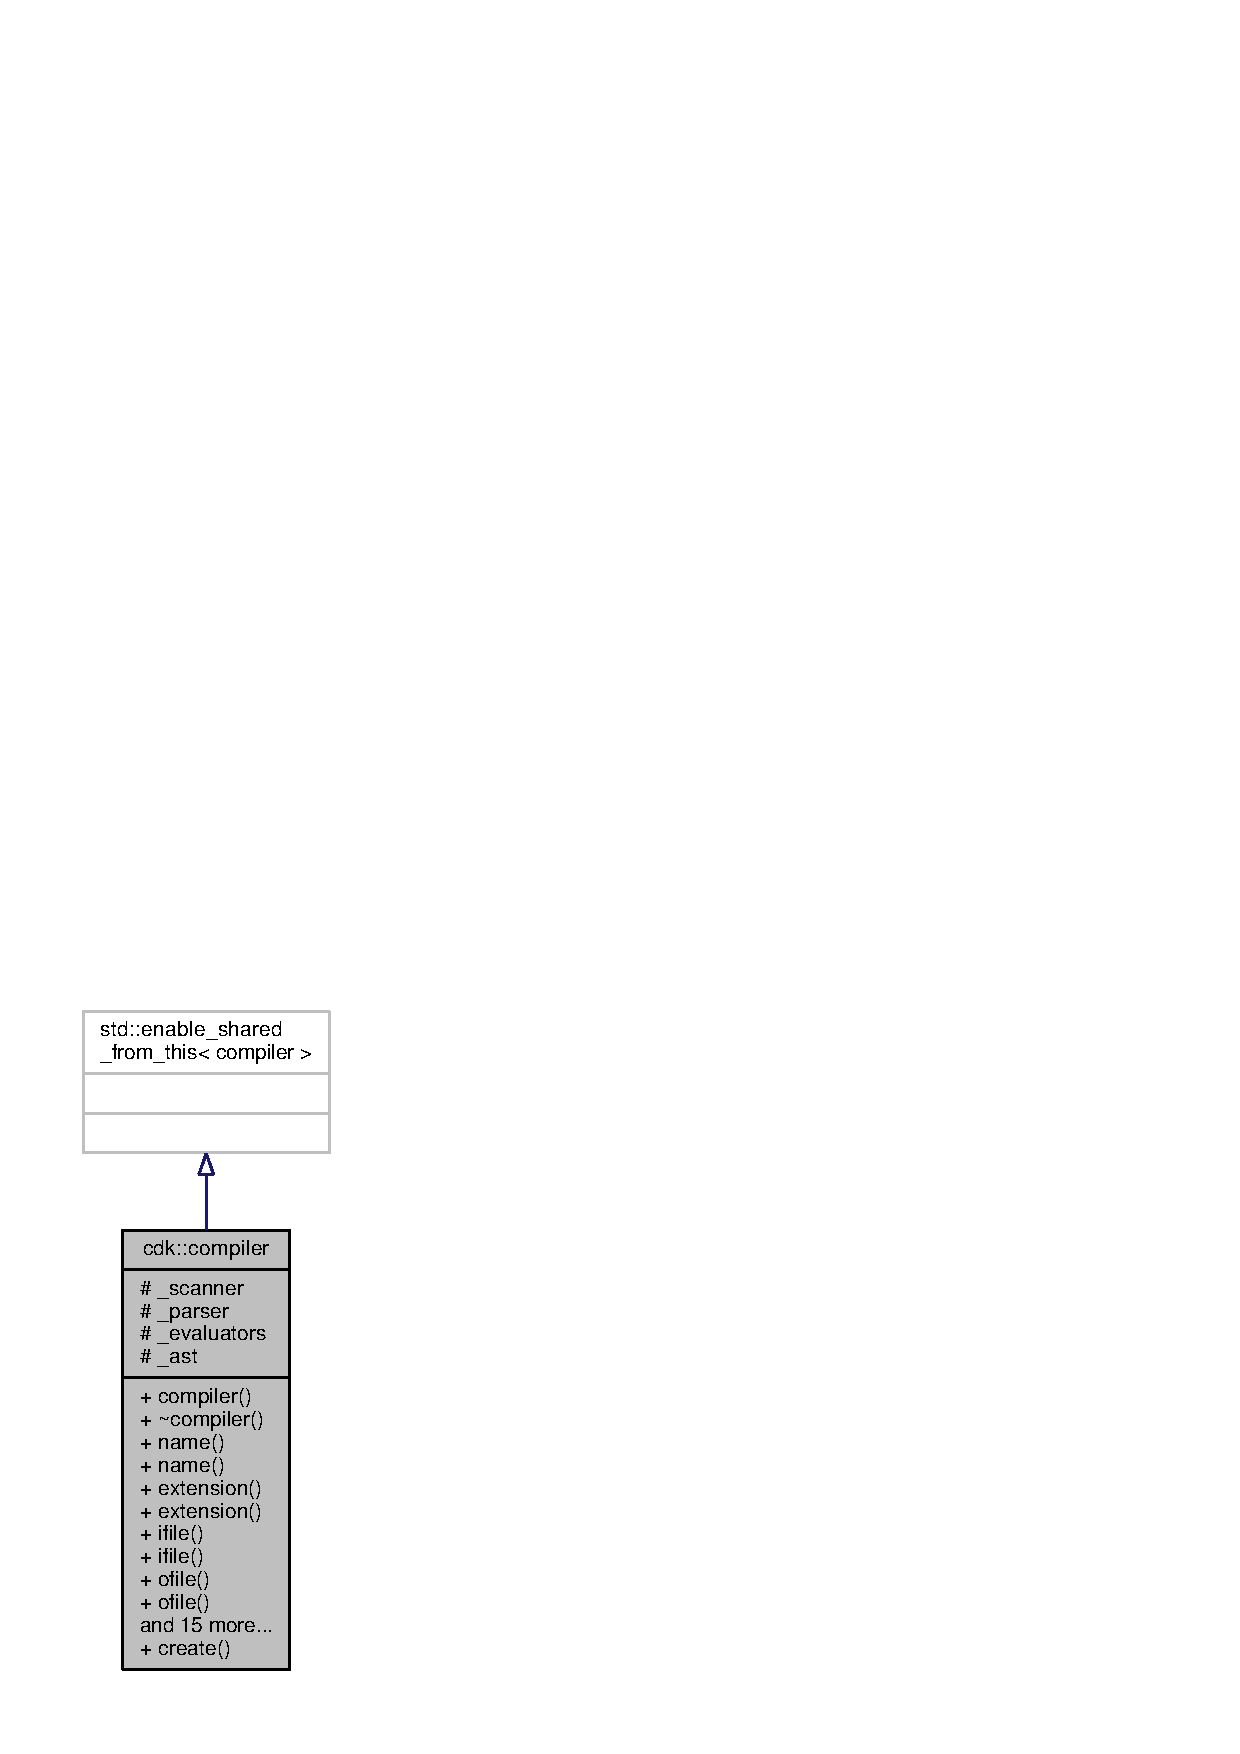
\includegraphics[width=162pt]{classcdk_1_1compiler__inherit__graph}
\end{center}
\end{figure}


Collaboration diagram for cdk\+:\+:compiler\+:
\nopagebreak
\begin{figure}[H]
\begin{center}
\leavevmode
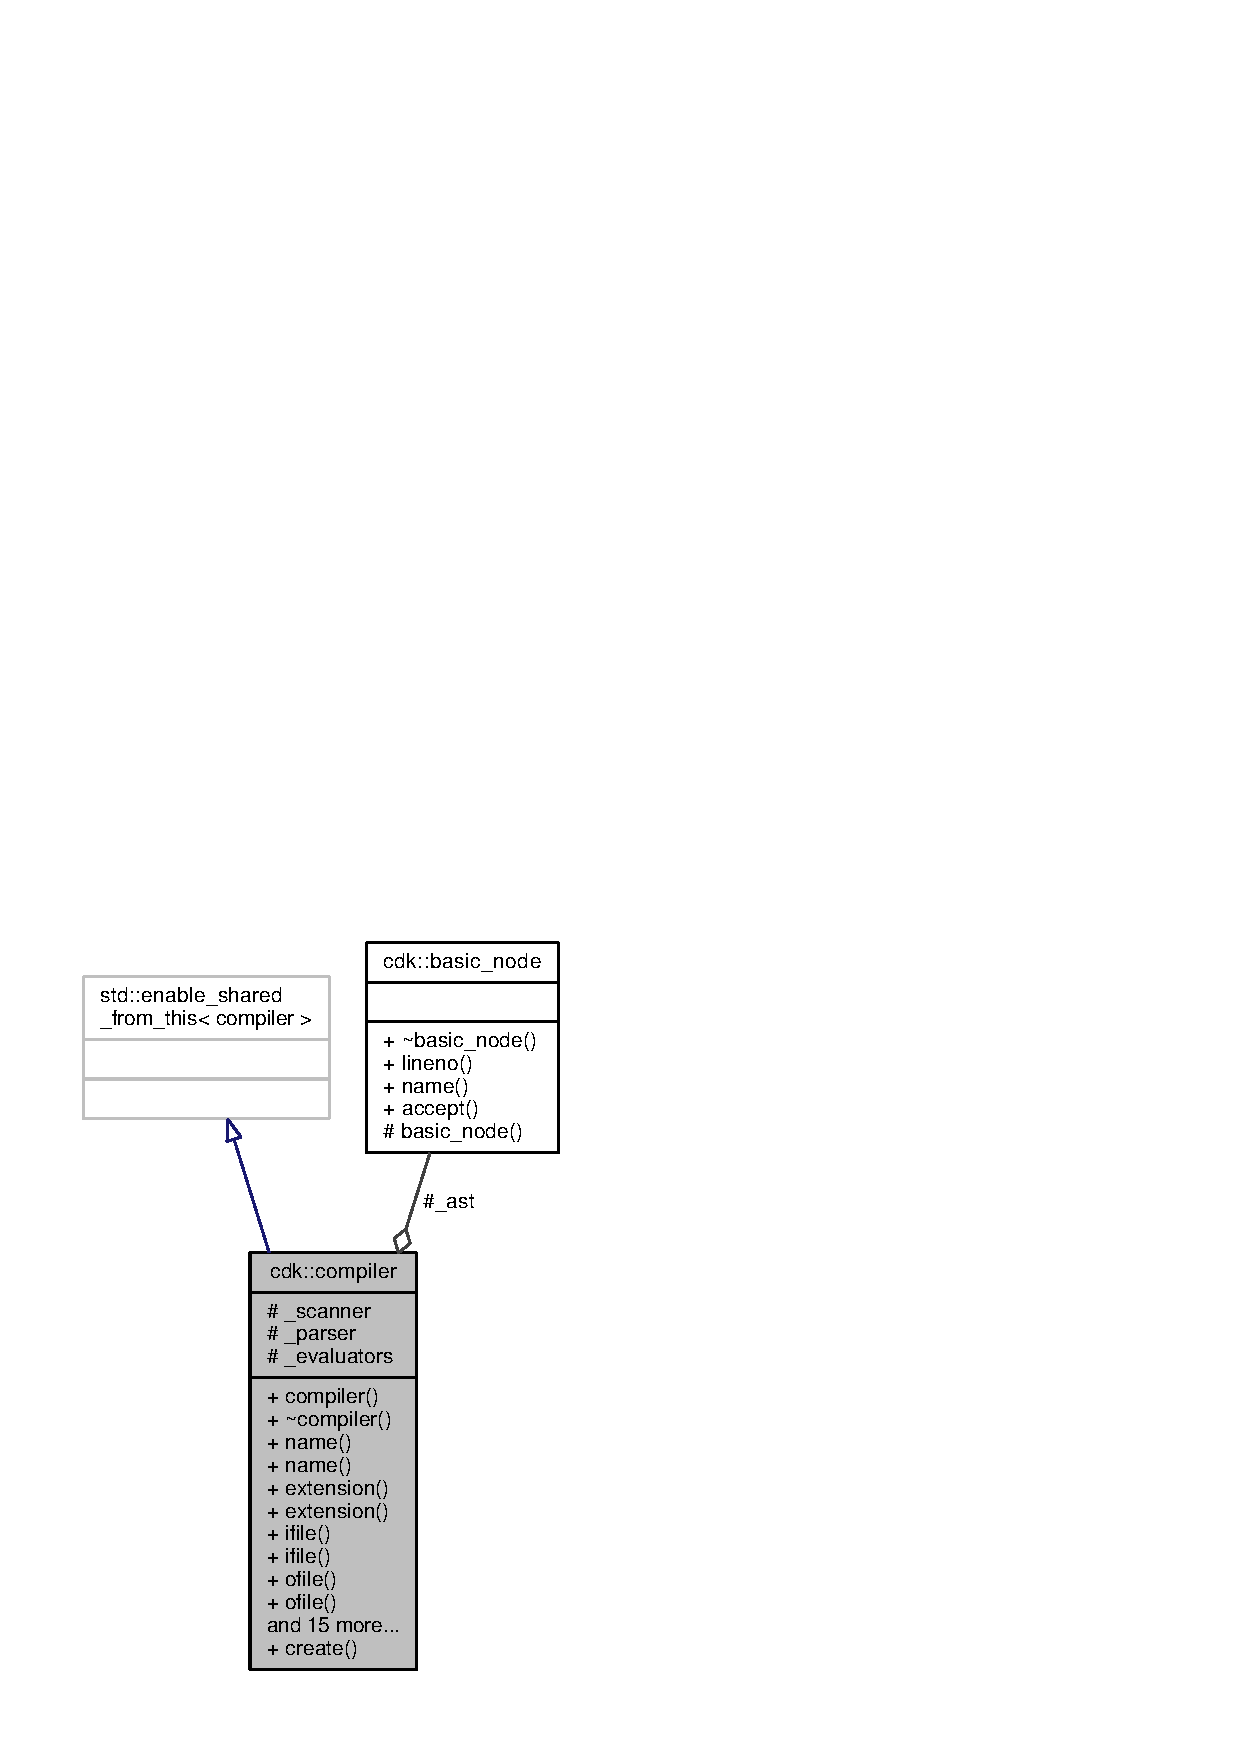
\includegraphics[width=272pt]{classcdk_1_1compiler__coll__graph}
\end{center}
\end{figure}
\subsection*{Public Member Functions}
\begin{DoxyCompactItemize}
\item 
{\bfseries compiler} (const std\+::string \&language, std\+::shared\+\_\+ptr$<$ {\bf basic\+\_\+scanner} $>$ scanner, std\+::shared\+\_\+ptr$<$ {\bf basic\+\_\+parser} $>$ parser)\label{classcdk_1_1compiler_a0718890212e30c490d31158ea8d75f73}

\item 
const std\+::string \& {\bfseries name} () const \label{classcdk_1_1compiler_a15f8502422151ac34bcaaa78790cfa41}

\item 
void {\bfseries name} (const std\+::string \&name)\label{classcdk_1_1compiler_a933cbe2e866df6bcf976f3b2bca53873}

\item 
const std\+::string \& {\bfseries extension} () const \label{classcdk_1_1compiler_a5f94c7de284d1b6eea8a8f613b177830}

\item 
void {\bfseries extension} (const std\+::string \&extension)\label{classcdk_1_1compiler_a944e52a202d89b3ba19988eacdc617b2}

\item 
const std\+::string \& {\bfseries ifile} () const \label{classcdk_1_1compiler_a7477c2ec092266198bdecdedb198f2ed}

\item 
void {\bfseries ifile} (const std\+::string \&ifile)\label{classcdk_1_1compiler_ac7a952f66fed4125e3054b5c7592ddb1}

\item 
const std\+::string \& {\bfseries ofile} () const \label{classcdk_1_1compiler_a1b372fc1814ae74cd4dcb36aefb86705}

\item 
void {\bfseries ofile} (const std\+::string \&ofile)\label{classcdk_1_1compiler_a2077beaf9b1bc9d087830d609a397de5}

\item 
std\+::shared\+\_\+ptr$<$ std\+::istream $>$ {\bfseries istream} ()\label{classcdk_1_1compiler_ae7cf9a49176b0ab9239f0c4d2e5b1668}

\item 
std\+::shared\+\_\+ptr$<$ std\+::ostream $>$ {\bfseries ostream} ()\label{classcdk_1_1compiler_a36a108cb45b06e37eca6dfc4075784fa}

\item 
{\bf basic\+\_\+node} $\ast$ {\bfseries ast} ()\label{classcdk_1_1compiler_ae95606d4deb9e5be056685b1f634d10f}

\item 
void {\bfseries ast} ({\bf basic\+\_\+node} $\ast$ast)\label{classcdk_1_1compiler_a841837c96b96d9c59532e57982011dc0}

\item 
std\+::shared\+\_\+ptr$<$ {\bf basic\+\_\+scanner} $>$ {\bfseries scanner} ()\label{classcdk_1_1compiler_abc44fb2cd388b0c4f76e0797e0972ecf}

\item 
void {\bfseries scanner} (std\+::shared\+\_\+ptr$<$ {\bf basic\+\_\+scanner} $>$ scanner)\label{classcdk_1_1compiler_a4ee8a64e131f0fd1d179e8be8d88e654}

\item 
std\+::shared\+\_\+ptr$<$ {\bf basic\+\_\+parser} $>$ {\bfseries parser} ()\label{classcdk_1_1compiler_a701f3411ada26d678b133134f492e6dd}

\item 
void {\bfseries parser} (std\+::shared\+\_\+ptr$<$ {\bf basic\+\_\+parser} $>$ parser)\label{classcdk_1_1compiler_a52a6e6b5cfa7361ceb0372ef6b4a9f73}

\item 
bool {\bfseries optimize} () const \label{classcdk_1_1compiler_a0fae7c4f7f79d9fc48fbdfc872a75f73}

\item 
void {\bfseries optimize} (bool optimize)\label{classcdk_1_1compiler_afd34aede83f1a60e8f2685b7a9e31ffe}

\item 
bool {\bfseries debug} () const \label{classcdk_1_1compiler_a3b619e3c4583fe01ba1befc783908ad2}

\item 
void {\bfseries debug} (bool debug)\label{classcdk_1_1compiler_a672a0cd7f68b61956fdbd541b21445a1}

\item 
int {\bfseries errors} () const \label{classcdk_1_1compiler_a29b5ea1436004c2b14789091b96969db}

\item 
int {\bfseries parse} ()\label{classcdk_1_1compiler_a1f39738f2142ebdabfc2122b635fa9d7}

\item 
bool {\bf evaluate} ()
\end{DoxyCompactItemize}
\subsection*{Static Public Member Functions}
\begin{DoxyCompactItemize}
\item 
static std\+::shared\+\_\+ptr$<$ {\bf compiler} $>$ {\bfseries create} (const std\+::string \&language, std\+::shared\+\_\+ptr$<$ {\bf basic\+\_\+scanner} $>$ scanner, std\+::shared\+\_\+ptr$<$ {\bf basic\+\_\+parser} $>$ parser)\label{classcdk_1_1compiler_a0e14073a550646ab3ffeb20ec2c31691}

\end{DoxyCompactItemize}
\subsection*{Protected Attributes}
\begin{DoxyCompactItemize}
\item 
std\+::shared\+\_\+ptr$<$ {\bf basic\+\_\+scanner} $>$ {\bfseries \+\_\+scanner} = nullptr\label{classcdk_1_1compiler_aae1fd7a956e254db62736223f36abfe1}

\item 
std\+::shared\+\_\+ptr$<$ {\bf basic\+\_\+parser} $>$ {\bfseries \+\_\+parser} = nullptr\label{classcdk_1_1compiler_a4cf06cfabdd2a17f1f00c875cf67f27a}

\item 
std\+::vector$<$ std\+::shared\+\_\+ptr\\*
$<$ {\bf basic\+\_\+target} $>$ $>$ {\bfseries \+\_\+evaluators}\label{classcdk_1_1compiler_a1effd69d16b8b813ee1abfa47a9152cb}

\item 
{\bf basic\+\_\+node} $\ast$ {\bfseries \+\_\+ast}\label{classcdk_1_1compiler_a9d9ee8c3f17a0c87ba64f3e86aa7e52f}

\end{DoxyCompactItemize}


\subsection{Detailed Description}


Definition at line 20 of file compiler.\+h.



\subsection{Member Function Documentation}
\index{cdk\+::compiler@{cdk\+::compiler}!evaluate@{evaluate}}
\index{evaluate@{evaluate}!cdk\+::compiler@{cdk\+::compiler}}
\subsubsection[{evaluate}]{\setlength{\rightskip}{0pt plus 5cm}bool cdk\+::compiler\+::evaluate (
\begin{DoxyParamCaption}
{}
\end{DoxyParamCaption}
)\hspace{0.3cm}{\ttfamily [inline]}}\label{classcdk_1_1compiler_a0c0d48f8b1101bb17bd1908785d62eff}
Processes the A\+S\+T and produces the output file. The specific processing strategy is provided independently by each back-\/end implementation (evaluator subclasses). 

Definition at line 189 of file compiler.\+h.



References cdk\+::basic\+\_\+target\+::evaluate(), and cdk\+::basic\+\_\+target\+::get\+\_\+target\+\_\+for().



Here is the call graph for this function\+:
\nopagebreak
\begin{figure}[H]
\begin{center}
\leavevmode
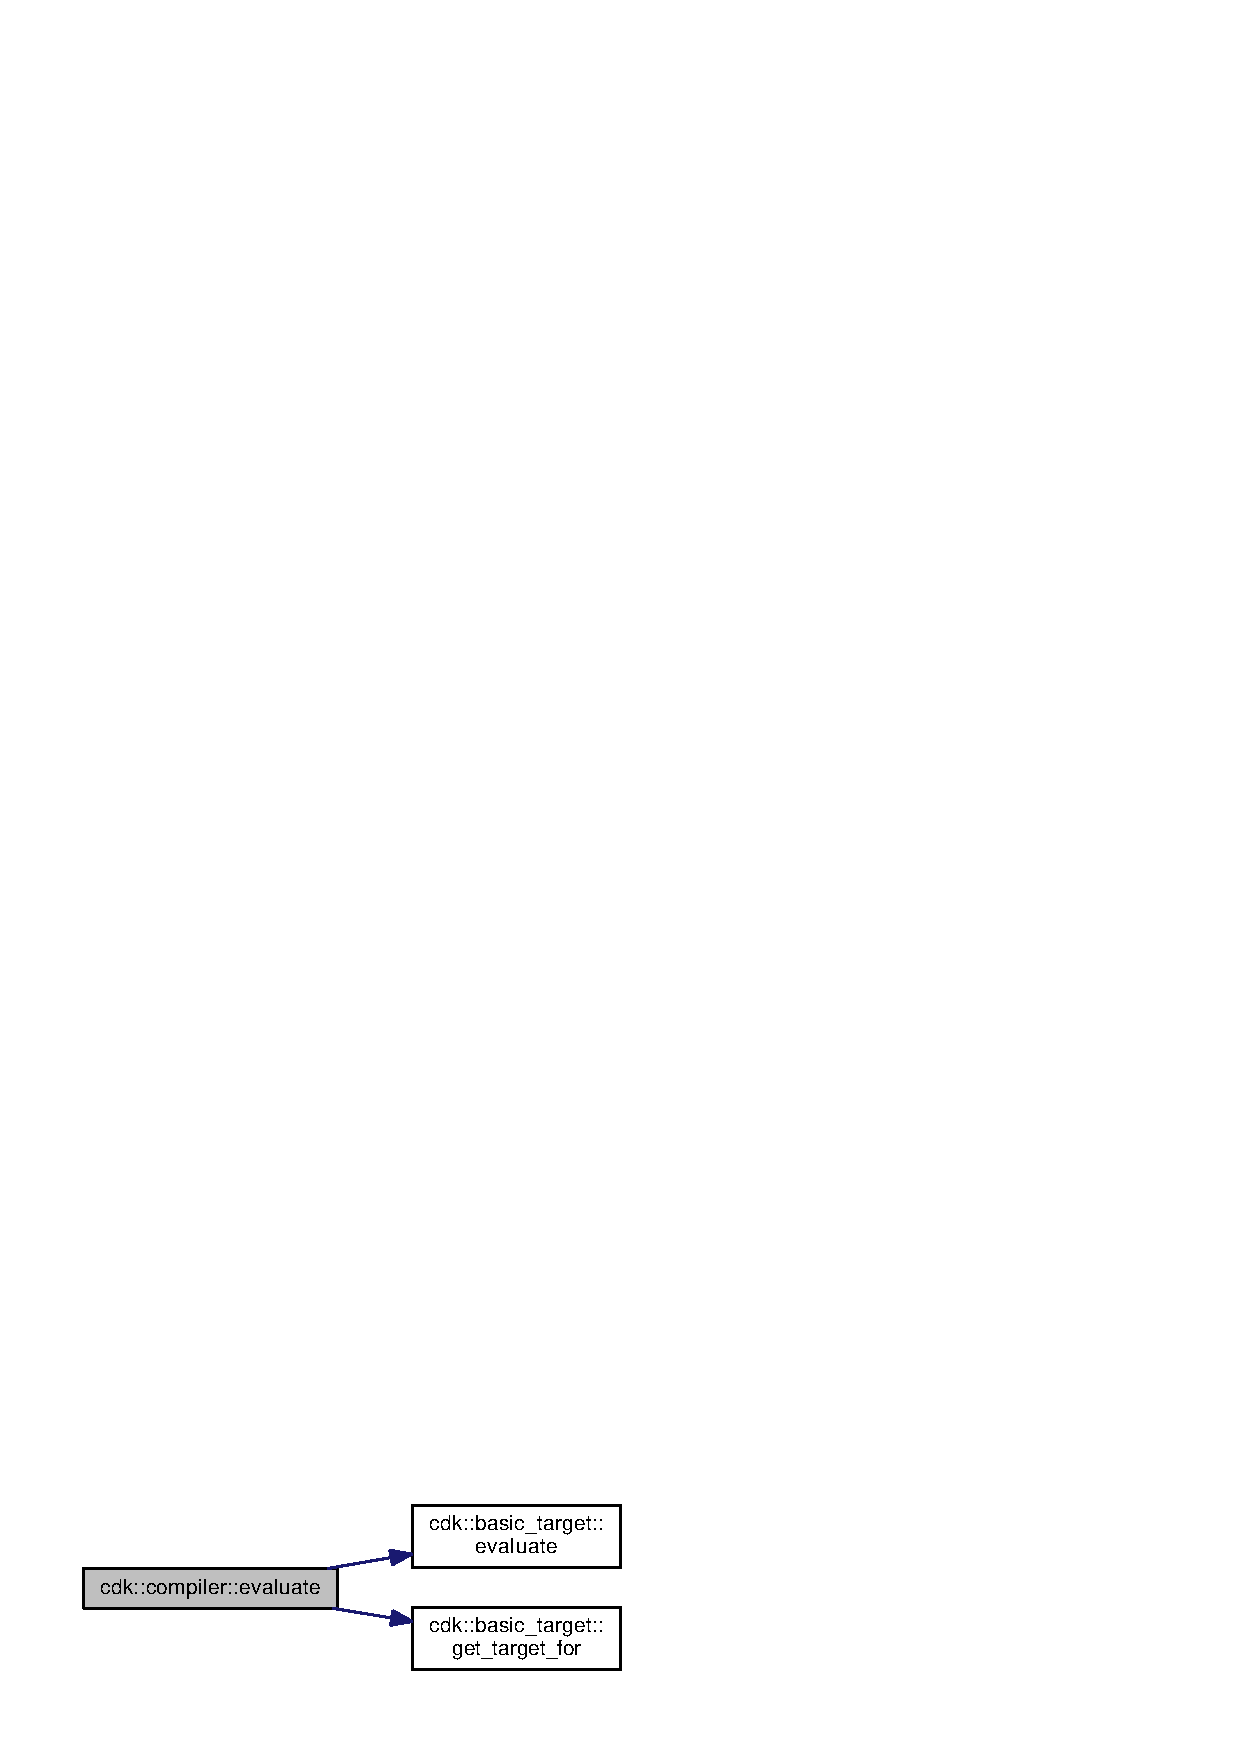
\includegraphics[width=302pt]{classcdk_1_1compiler_a0c0d48f8b1101bb17bd1908785d62eff_cgraph}
\end{center}
\end{figure}




The documentation for this class was generated from the following file\+:\begin{DoxyCompactItemize}
\item 
compiler.\+h\end{DoxyCompactItemize}

\section{cdk\+:\+:composite\+\_\+node Class Reference}
\label{classcdk_1_1composite__node}\index{cdk\+::composite\+\_\+node@{cdk\+::composite\+\_\+node}}


Inheritance diagram for cdk\+:\+:composite\+\_\+node\+:
\nopagebreak
\begin{figure}[H]
\begin{center}
\leavevmode
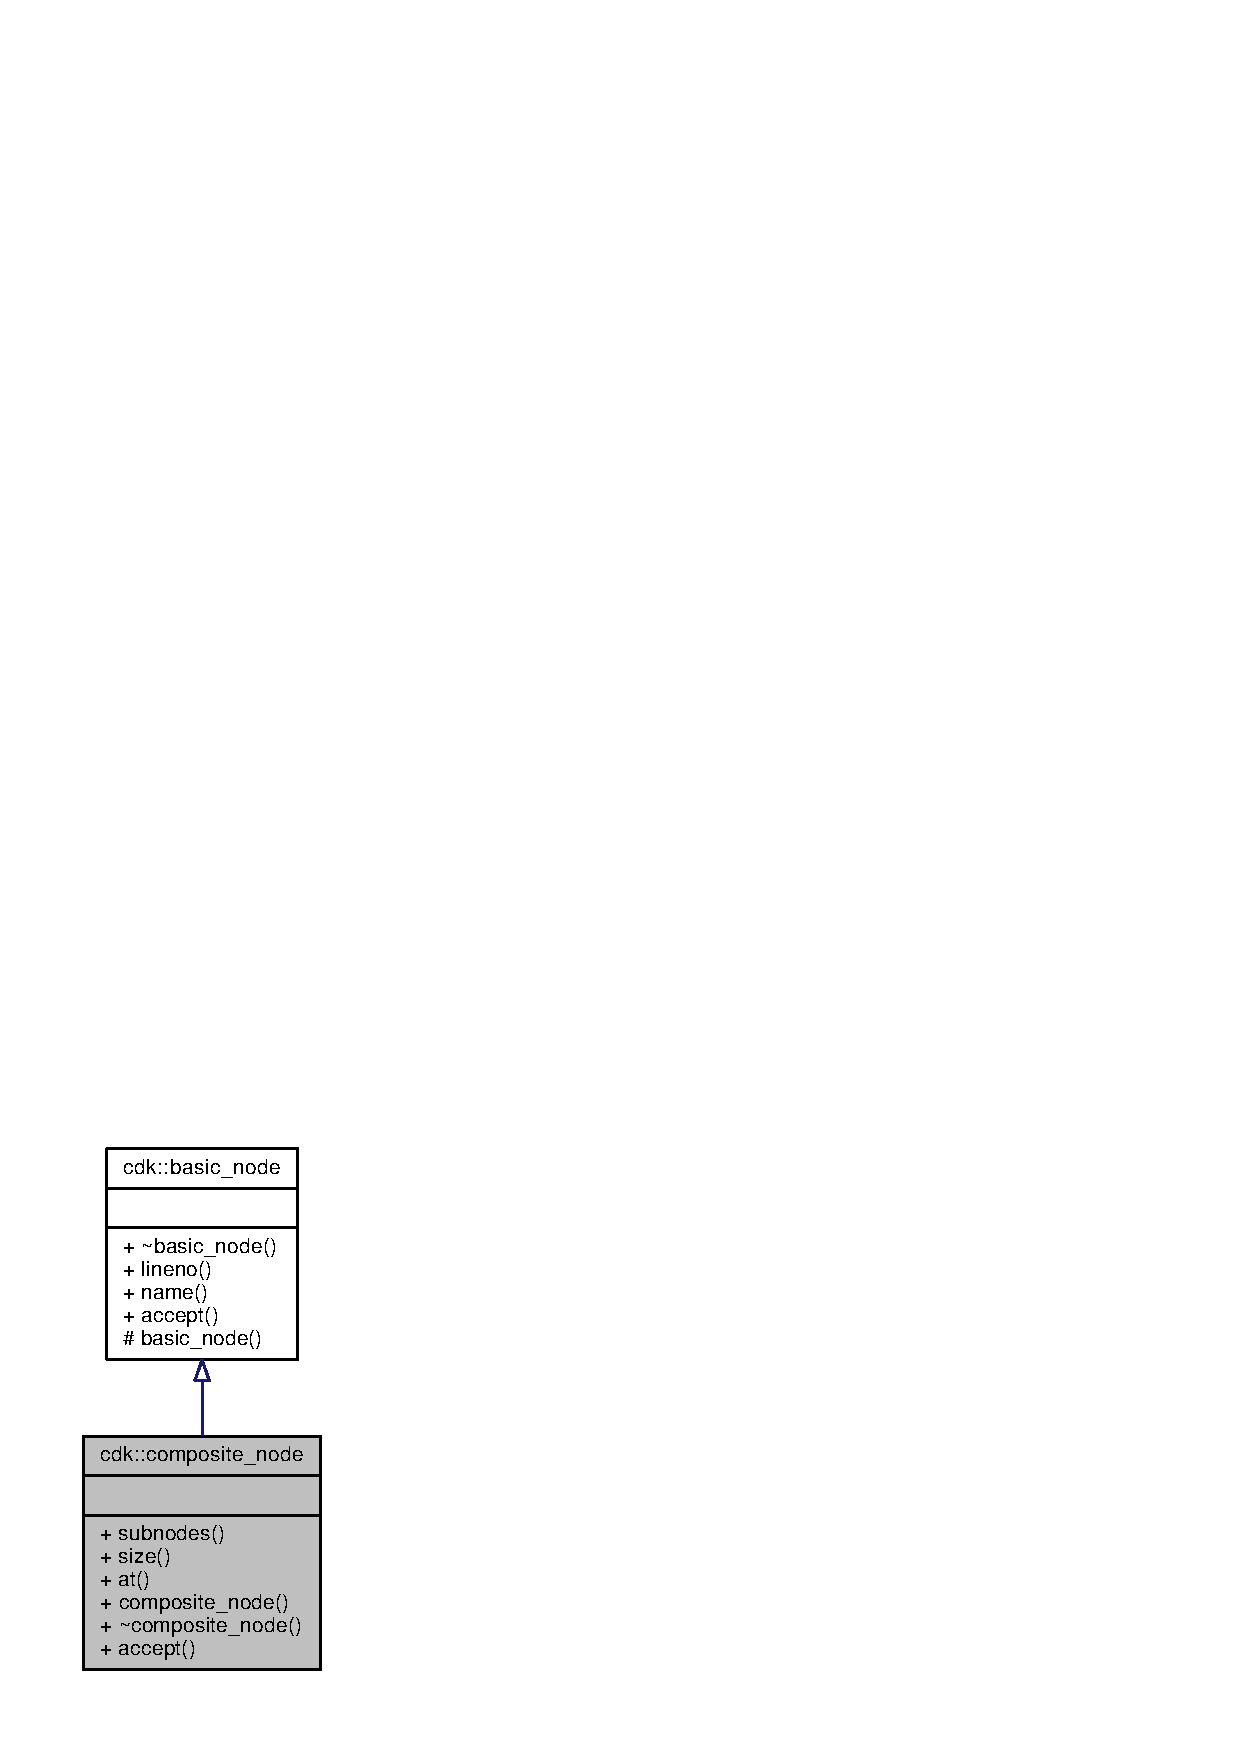
\includegraphics[width=158pt]{classcdk_1_1composite__node__inherit__graph}
\end{center}
\end{figure}


Collaboration diagram for cdk\+:\+:composite\+\_\+node\+:
\nopagebreak
\begin{figure}[H]
\begin{center}
\leavevmode
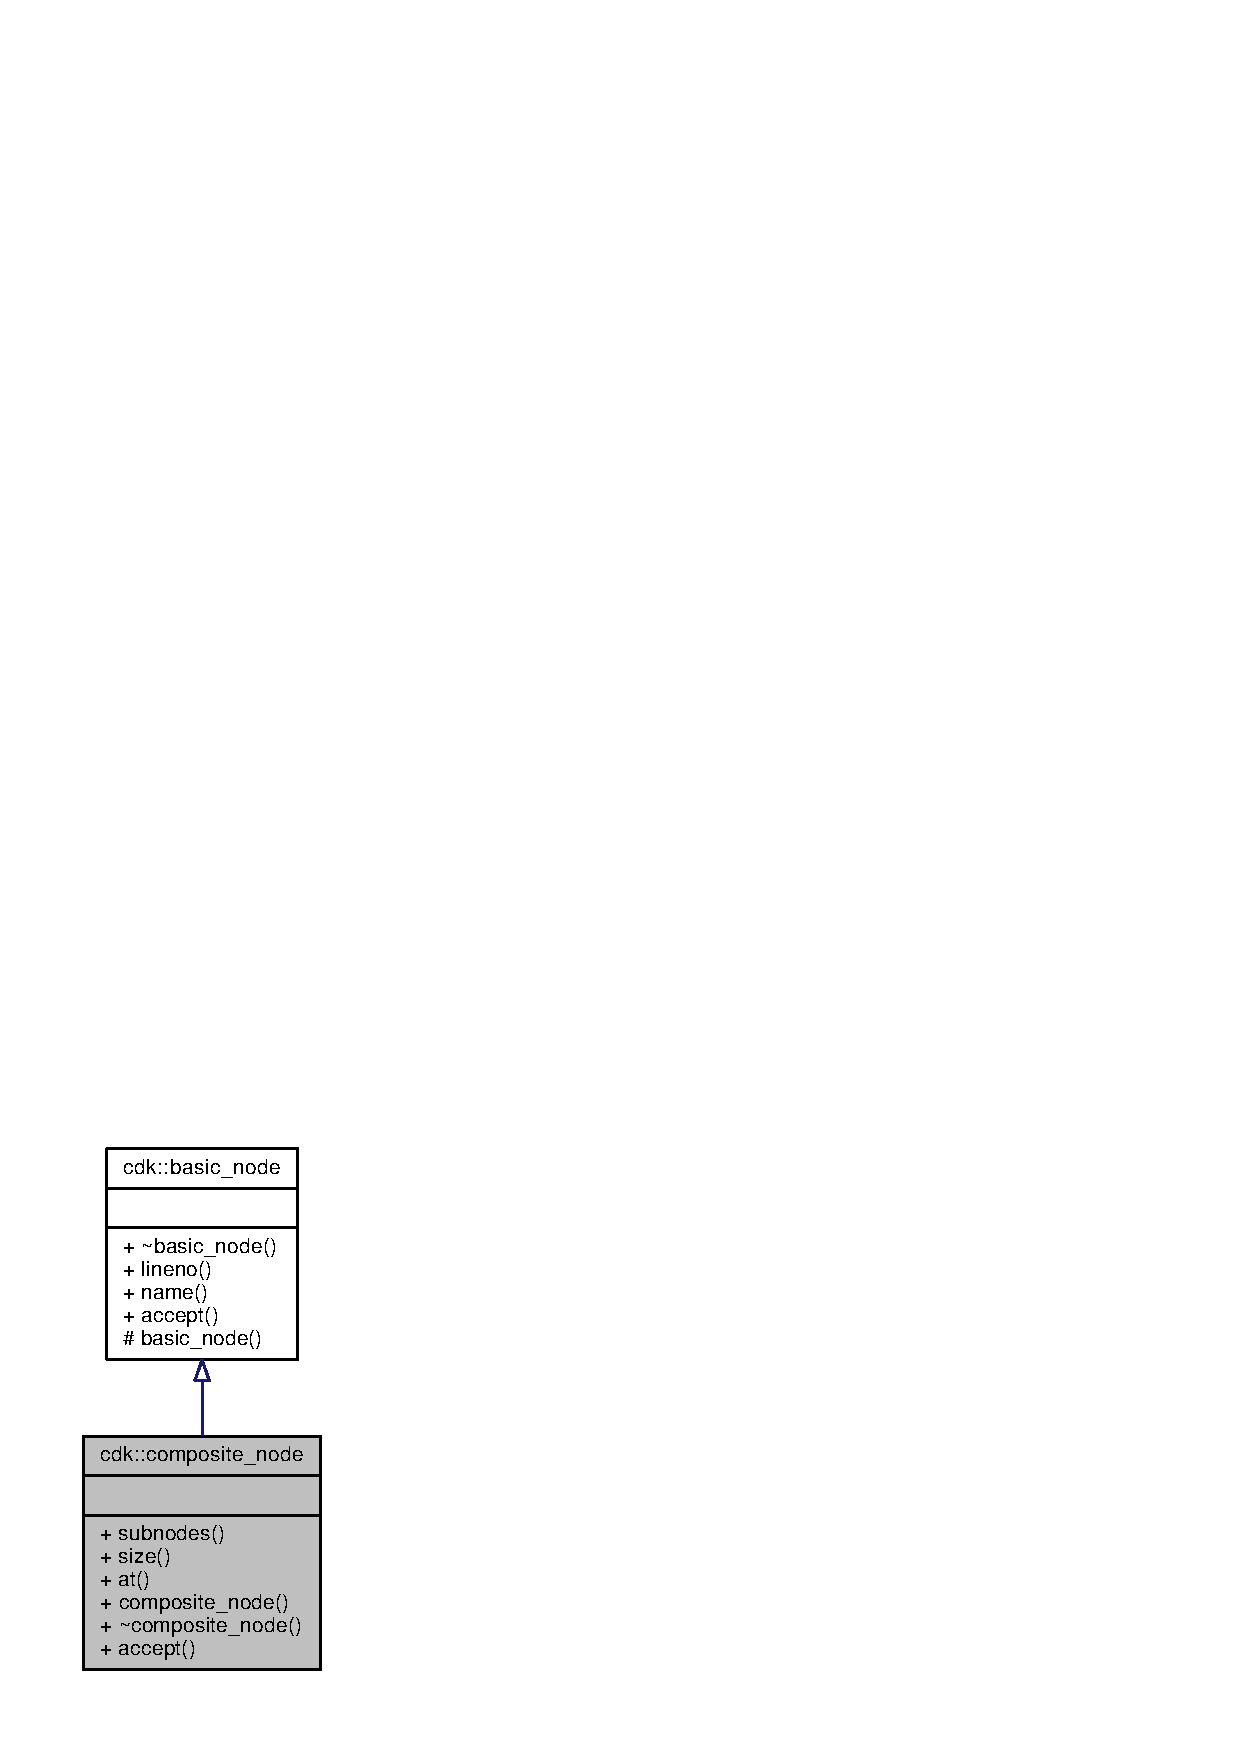
\includegraphics[width=158pt]{classcdk_1_1composite__node__coll__graph}
\end{center}
\end{figure}
\subsection*{Public Member Functions}
\begin{DoxyCompactItemize}
\item 
std\+::vector$<$ {\bf basic\+\_\+node} $\ast$ $>$ \& {\bfseries subnodes} ()\label{classcdk_1_1composite__node_aa06e19a09122ee3adc47eb6ed5154864}

\item 
size\+\_\+t {\bfseries size} ()\label{classcdk_1_1composite__node_a51c0c078759cf3b6827d3739ffd80463}

\item 
{\bf basic\+\_\+node} $\ast$ {\bfseries at} (size\+\_\+t i)\label{classcdk_1_1composite__node_a5496f0b49a5ef8ea118ba27dfb640015}

\item 
{\bf composite\+\_\+node} (int {\bf lineno}, int nops,...)
\item 
{\bf $\sim$composite\+\_\+node} ()
\item 
void {\bf accept} ({\bf basic\+\_\+ast\+\_\+visitor} $\ast$sp, int level)
\end{DoxyCompactItemize}
\subsection*{Additional Inherited Members}


\subsection{Detailed Description}


Definition at line 11 of file composite\+\_\+node.\+h.



\subsection{Constructor \& Destructor Documentation}
\index{cdk\+::composite\+\_\+node@{cdk\+::composite\+\_\+node}!composite\+\_\+node@{composite\+\_\+node}}
\index{composite\+\_\+node@{composite\+\_\+node}!cdk\+::composite\+\_\+node@{cdk\+::composite\+\_\+node}}
\subsubsection[{composite\+\_\+node}]{\setlength{\rightskip}{0pt plus 5cm}cdk\+::composite\+\_\+node\+::composite\+\_\+node (
\begin{DoxyParamCaption}
\item[{int}]{lineno, }
\item[{int}]{nops, }
\item[{}]{...}
\end{DoxyParamCaption}
)\hspace{0.3cm}{\ttfamily [inline]}}\label{classcdk_1_1composite__node_a3834fb5b7f00fdf5a89b2504b06a322b}
The constructor of a composite node takes the same first argument as any other node. The second argument is the number of child nodes\+: this argument is followed by the child nodes themselves. Note that no effort is made to ensure that the given number of children matches the actual children passed to the function. {\bfseries You have been warned...}


\begin{DoxyParams}{Parameters}
{\em lineno} & the source code line number that originated the node \\
\hline
{\em nops} & the number of child nodes \\
\hline
{\em ...} & the child nodes \\
\hline
\end{DoxyParams}


Definition at line 39 of file composite\+\_\+node.\+h.

\index{cdk\+::composite\+\_\+node@{cdk\+::composite\+\_\+node}!````~composite\+\_\+node@{$\sim$composite\+\_\+node}}
\index{````~composite\+\_\+node@{$\sim$composite\+\_\+node}!cdk\+::composite\+\_\+node@{cdk\+::composite\+\_\+node}}
\subsubsection[{$\sim$composite\+\_\+node}]{\setlength{\rightskip}{0pt plus 5cm}cdk\+::composite\+\_\+node\+::$\sim$composite\+\_\+node (
\begin{DoxyParamCaption}
{}
\end{DoxyParamCaption}
)\hspace{0.3cm}{\ttfamily [inline]}}\label{classcdk_1_1composite__node_ab0ee2b262c7b6b55a9ddb052be60b648}
This is the destructor for composite nodes. Note that this destructor also causes the destruction of the node's children. 

Definition at line 54 of file composite\+\_\+node.\+h.



\subsection{Member Function Documentation}
\index{cdk\+::composite\+\_\+node@{cdk\+::composite\+\_\+node}!accept@{accept}}
\index{accept@{accept}!cdk\+::composite\+\_\+node@{cdk\+::composite\+\_\+node}}
\subsubsection[{accept}]{\setlength{\rightskip}{0pt plus 5cm}void cdk\+::composite\+\_\+node\+::accept (
\begin{DoxyParamCaption}
\item[{{\bf basic\+\_\+ast\+\_\+visitor} $\ast$}]{sp, }
\item[{int}]{level}
\end{DoxyParamCaption}
)\hspace{0.3cm}{\ttfamily [inline]}, {\ttfamily [virtual]}}\label{classcdk_1_1composite__node_af7ac243ab23b1204c44010cf42ef14a2}

\begin{DoxyParams}{Parameters}
{\em sp} & semantic processor visitor \\
\hline
{\em level} & syntactic tree level \\
\hline
\end{DoxyParams}


Implements {\bf cdk\+::basic\+\_\+node} \doxyref{}{p.}{classcdk_1_1basic__node_ab38adcbc95c46b809961278afae3bf05}.



Definition at line 64 of file composite\+\_\+node.\+h.



The documentation for this class was generated from the following file\+:\begin{DoxyCompactItemize}
\item 
ast/composite\+\_\+node.\+h\end{DoxyCompactItemize}

\section{cdk\+:\+:data\+\_\+node Class Reference}
\label{classcdk_1_1data__node}\index{cdk\+::data\+\_\+node@{cdk\+::data\+\_\+node}}


{\ttfamily \#include $<$data\+\_\+node.\+h$>$}



Inheritance diagram for cdk\+:\+:data\+\_\+node\+:
\nopagebreak
\begin{figure}[H]
\begin{center}
\leavevmode
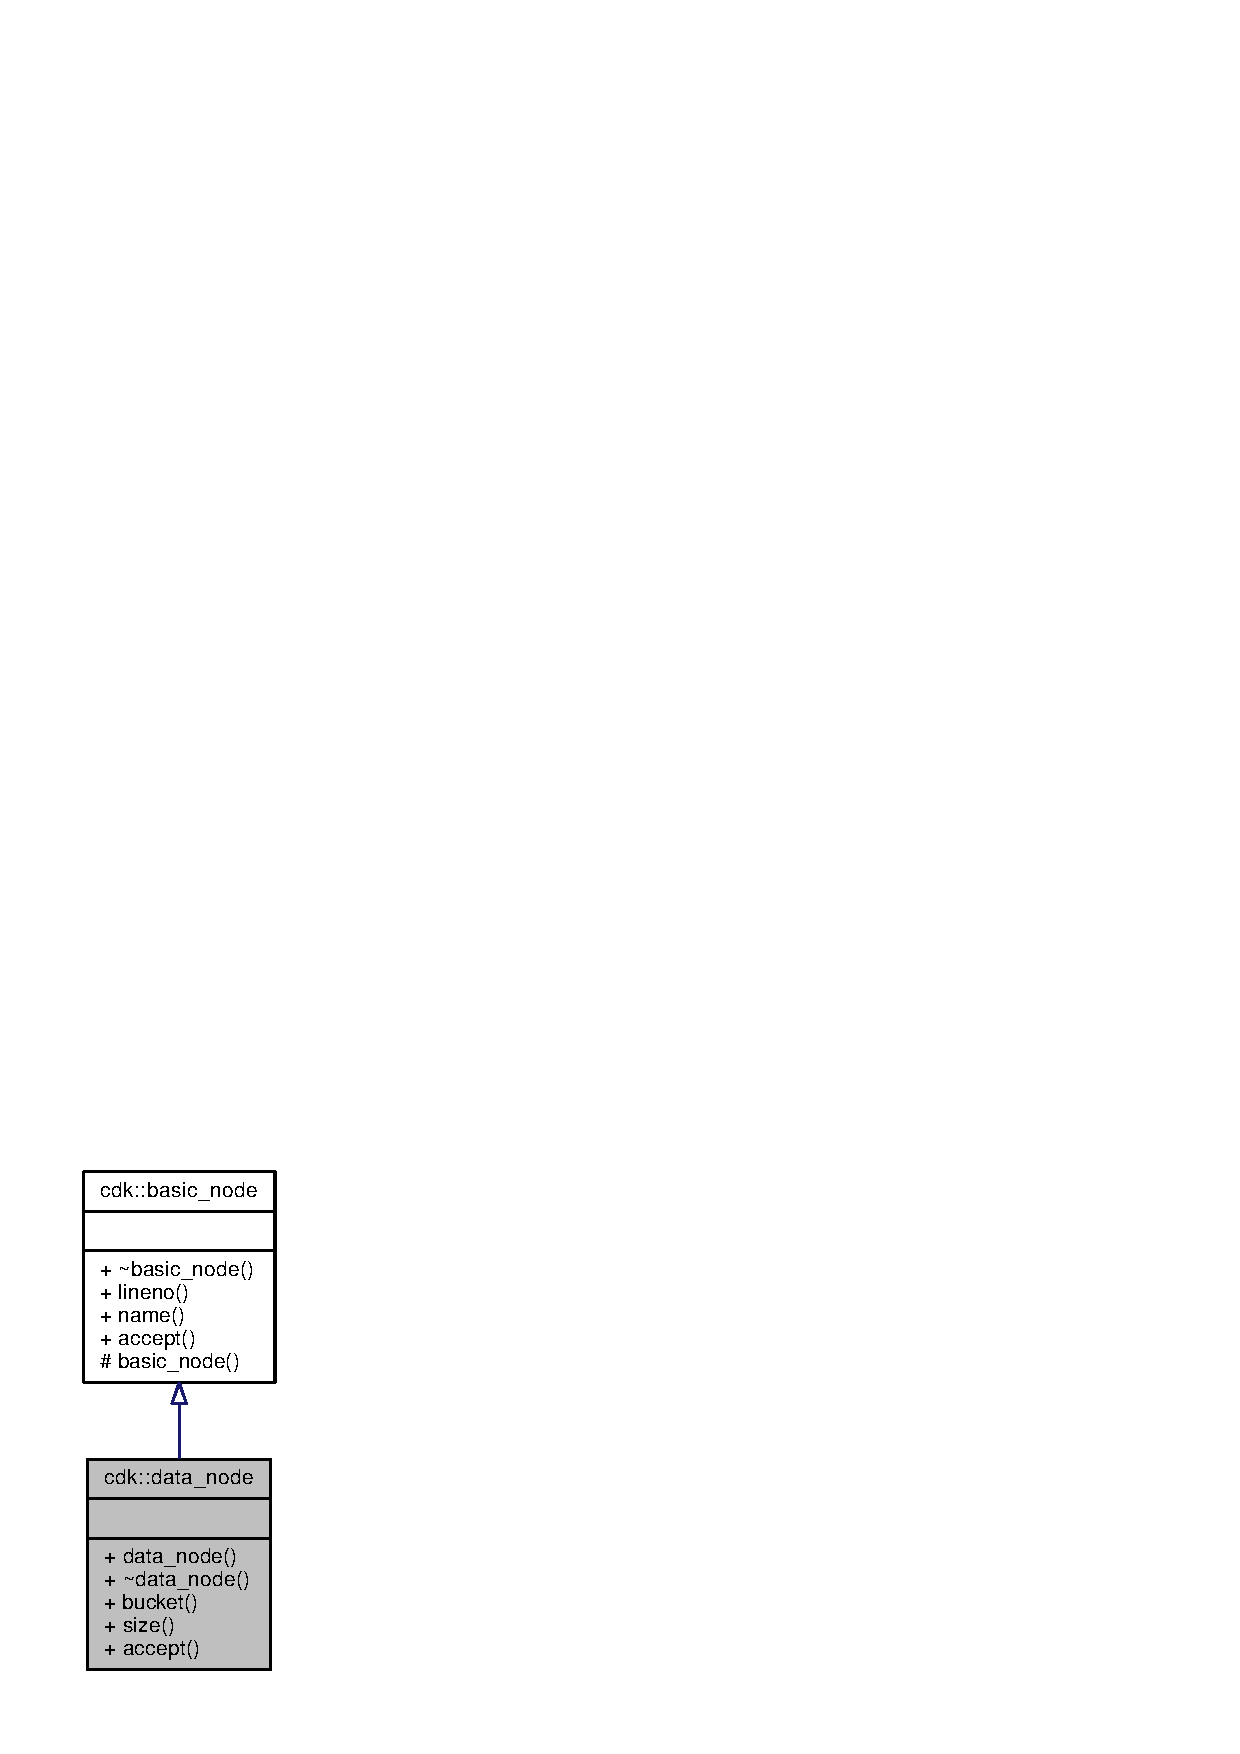
\includegraphics[width=136pt]{classcdk_1_1data__node__inherit__graph}
\end{center}
\end{figure}


Collaboration diagram for cdk\+:\+:data\+\_\+node\+:
\nopagebreak
\begin{figure}[H]
\begin{center}
\leavevmode
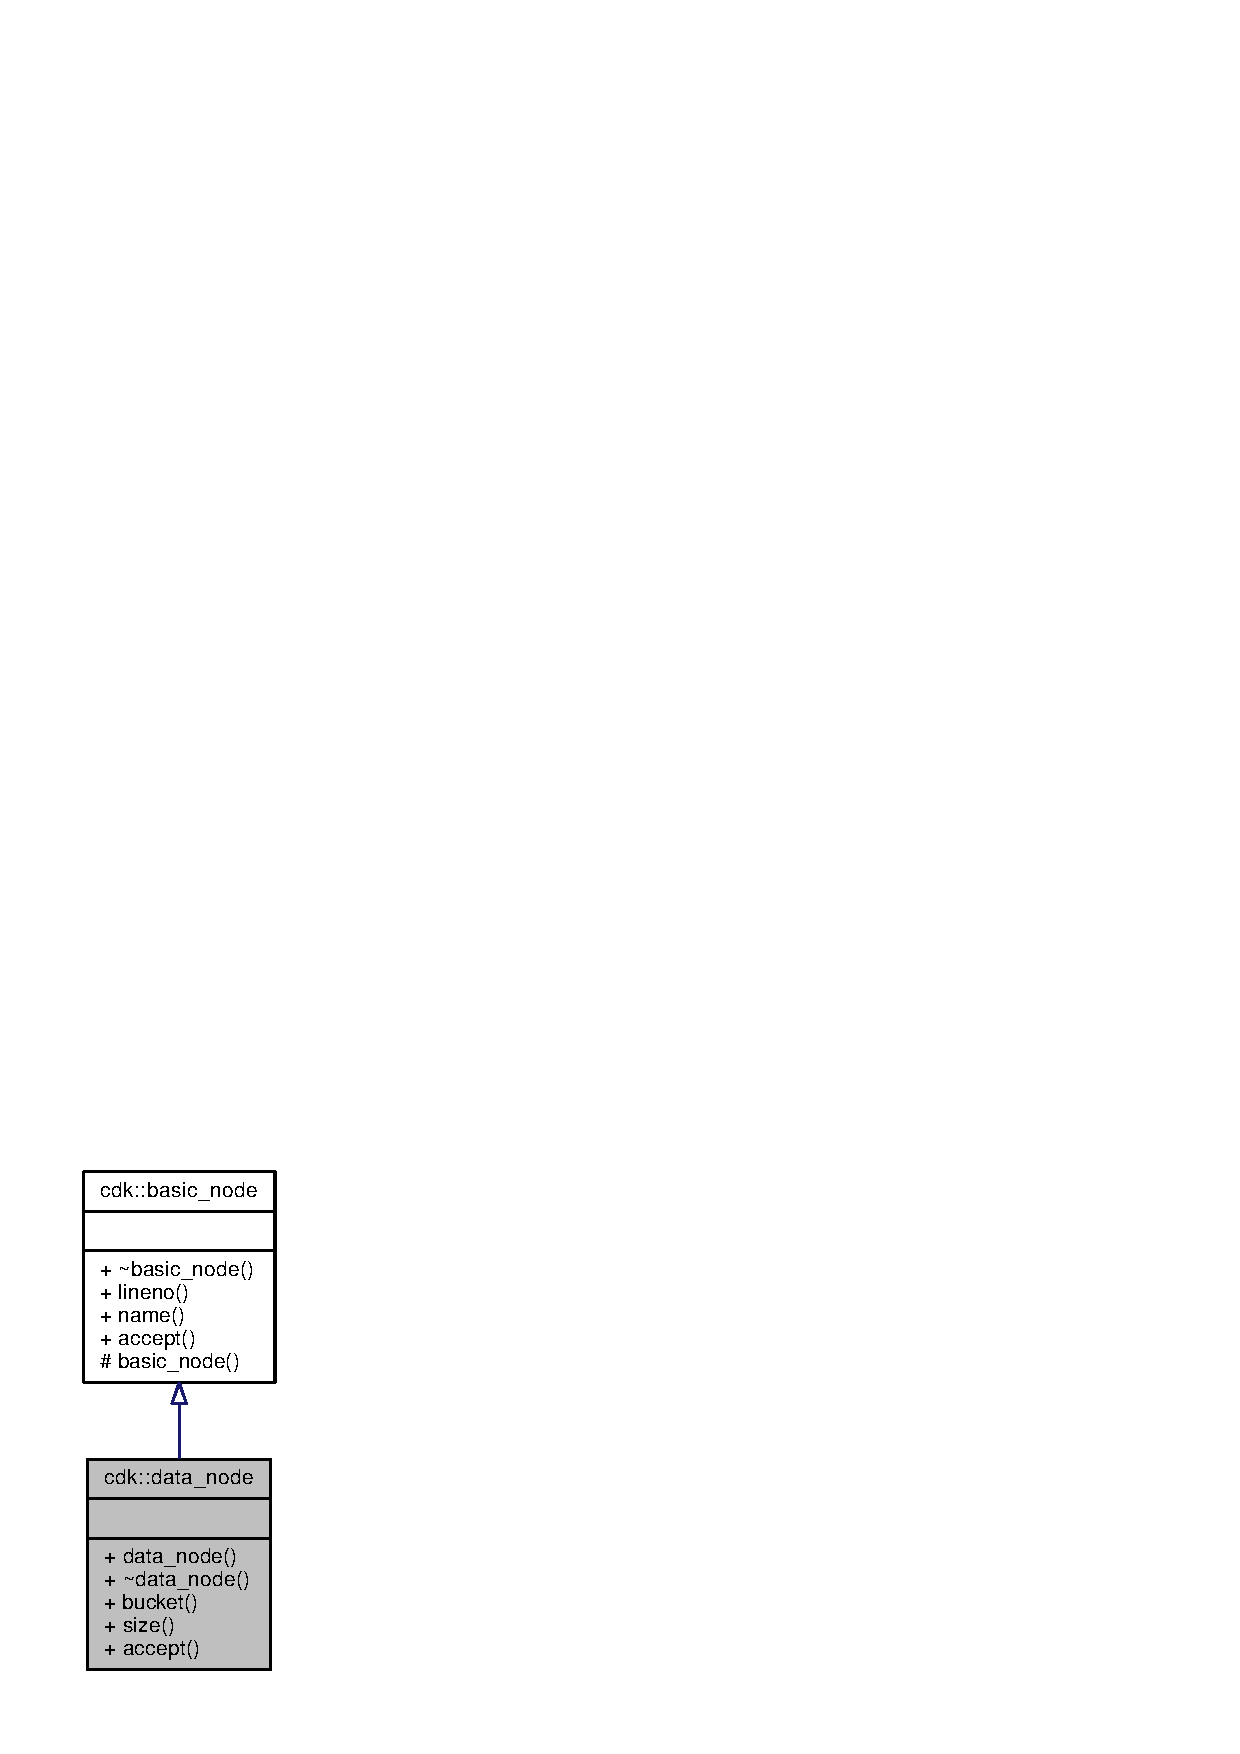
\includegraphics[width=136pt]{classcdk_1_1data__node__coll__graph}
\end{center}
\end{figure}
\subsection*{Public Member Functions}
\begin{DoxyCompactItemize}
\item 
{\bf data\+\_\+node} (int {\bf lineno}, void $\ast$data, size\+\_\+t nbytes)
\item 
{\bf $\sim$data\+\_\+node} ()
\item 
void $\ast$ {\bfseries bucket} ()\label{classcdk_1_1data__node_a6b68a4bf2fdbce288421128d9c980944}

\item 
size\+\_\+t {\bfseries size} ()\label{classcdk_1_1data__node_a14645461b55cd730f23e95f5ae023bb6}

\item 
void {\bf accept} ({\bf basic\+\_\+ast\+\_\+visitor} $\ast$sp, int level)
\end{DoxyCompactItemize}
\subsection*{Additional Inherited Members}


\subsection{Detailed Description}
Class for describing syntactic tree leaves for holding data buffers. This class does not inherit from the {\ttfamily Simple} template. 

Definition at line 14 of file data\+\_\+node.\+h.



\subsection{Constructor \& Destructor Documentation}
\index{cdk\+::data\+\_\+node@{cdk\+::data\+\_\+node}!data\+\_\+node@{data\+\_\+node}}
\index{data\+\_\+node@{data\+\_\+node}!cdk\+::data\+\_\+node@{cdk\+::data\+\_\+node}}
\subsubsection[{data\+\_\+node}]{\setlength{\rightskip}{0pt plus 5cm}cdk\+::data\+\_\+node\+::data\+\_\+node (
\begin{DoxyParamCaption}
\item[{int}]{lineno, }
\item[{void $\ast$}]{data, }
\item[{size\+\_\+t}]{nbytes}
\end{DoxyParamCaption}
)\hspace{0.3cm}{\ttfamily [inline]}}\label{classcdk_1_1data__node_a28f06602d5b68131bed91f668545eb28}
Constructor for nodes that hold opaque data buffers. Each buffer is characterized by its data and the corresponding data size.


\begin{DoxyParams}{Parameters}
{\em lineno} & the source code line number corresponding to this node \\
\hline
{\em data} & the opaque data buffer \\
\hline
{\em nbytes} & the size (bytes) of the data buffer \\
\hline
\end{DoxyParams}


Definition at line 28 of file data\+\_\+node.\+h.

\index{cdk\+::data\+\_\+node@{cdk\+::data\+\_\+node}!````~data\+\_\+node@{$\sim$data\+\_\+node}}
\index{````~data\+\_\+node@{$\sim$data\+\_\+node}!cdk\+::data\+\_\+node@{cdk\+::data\+\_\+node}}
\subsubsection[{$\sim$data\+\_\+node}]{\setlength{\rightskip}{0pt plus 5cm}cdk\+::data\+\_\+node\+::$\sim$data\+\_\+node (
\begin{DoxyParamCaption}
{}
\end{DoxyParamCaption}
)\hspace{0.3cm}{\ttfamily [inline]}}\label{classcdk_1_1data__node_a196cea550b65cde781468694fecc2d9b}
The destructor. We have defined it explicitly (even though it was not needed) to emphasize that the data buffer is {\bfseries not} destroyed when the node itself dies. 

Definition at line 37 of file data\+\_\+node.\+h.



\subsection{Member Function Documentation}
\index{cdk\+::data\+\_\+node@{cdk\+::data\+\_\+node}!accept@{accept}}
\index{accept@{accept}!cdk\+::data\+\_\+node@{cdk\+::data\+\_\+node}}
\subsubsection[{accept}]{\setlength{\rightskip}{0pt plus 5cm}void cdk\+::data\+\_\+node\+::accept (
\begin{DoxyParamCaption}
\item[{{\bf basic\+\_\+ast\+\_\+visitor} $\ast$}]{sp, }
\item[{int}]{level}
\end{DoxyParamCaption}
)\hspace{0.3cm}{\ttfamily [inline]}, {\ttfamily [virtual]}}\label{classcdk_1_1data__node_a9d6d6f56201fdfbe965ec399ced60df8}

\begin{DoxyParams}{Parameters}
{\em sp} & semantic processor visitor \\
\hline
{\em level} & syntactic tree level \\
\hline
\end{DoxyParams}


Implements {\bf cdk\+::basic\+\_\+node} \doxyref{}{p.}{classcdk_1_1basic__node_ab38adcbc95c46b809961278afae3bf05}.



Definition at line 51 of file data\+\_\+node.\+h.



The documentation for this class was generated from the following file\+:\begin{DoxyCompactItemize}
\item 
ast/data\+\_\+node.\+h\end{DoxyCompactItemize}

\section{cdk\+:\+:div\+\_\+node Class Reference}
\label{classcdk_1_1div__node}\index{cdk\+::div\+\_\+node@{cdk\+::div\+\_\+node}}


{\ttfamily \#include $<$div\+\_\+node.\+h$>$}



Inheritance diagram for cdk\+:\+:div\+\_\+node\+:
\nopagebreak
\begin{figure}[H]
\begin{center}
\leavevmode
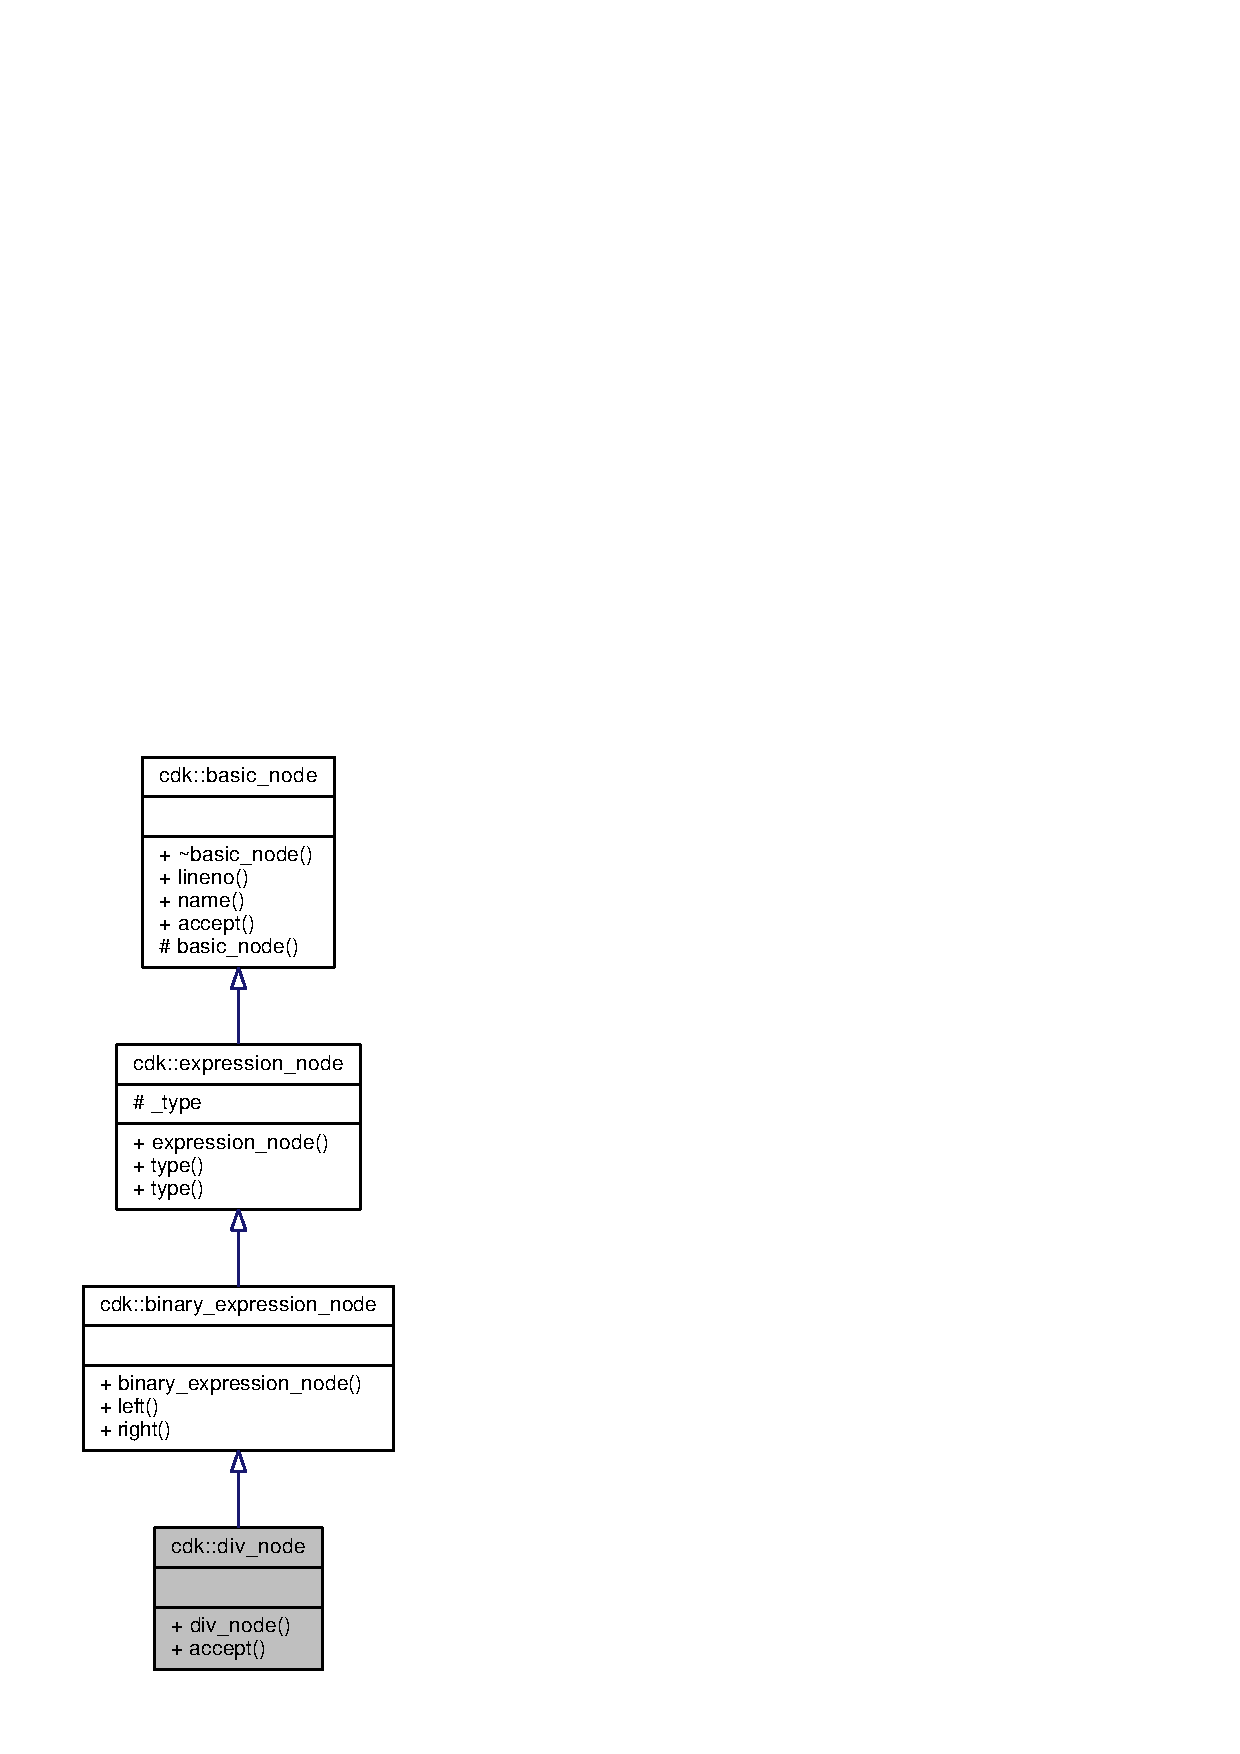
\includegraphics[width=193pt]{classcdk_1_1div__node__inherit__graph}
\end{center}
\end{figure}


Collaboration diagram for cdk\+:\+:div\+\_\+node\+:
\nopagebreak
\begin{figure}[H]
\begin{center}
\leavevmode
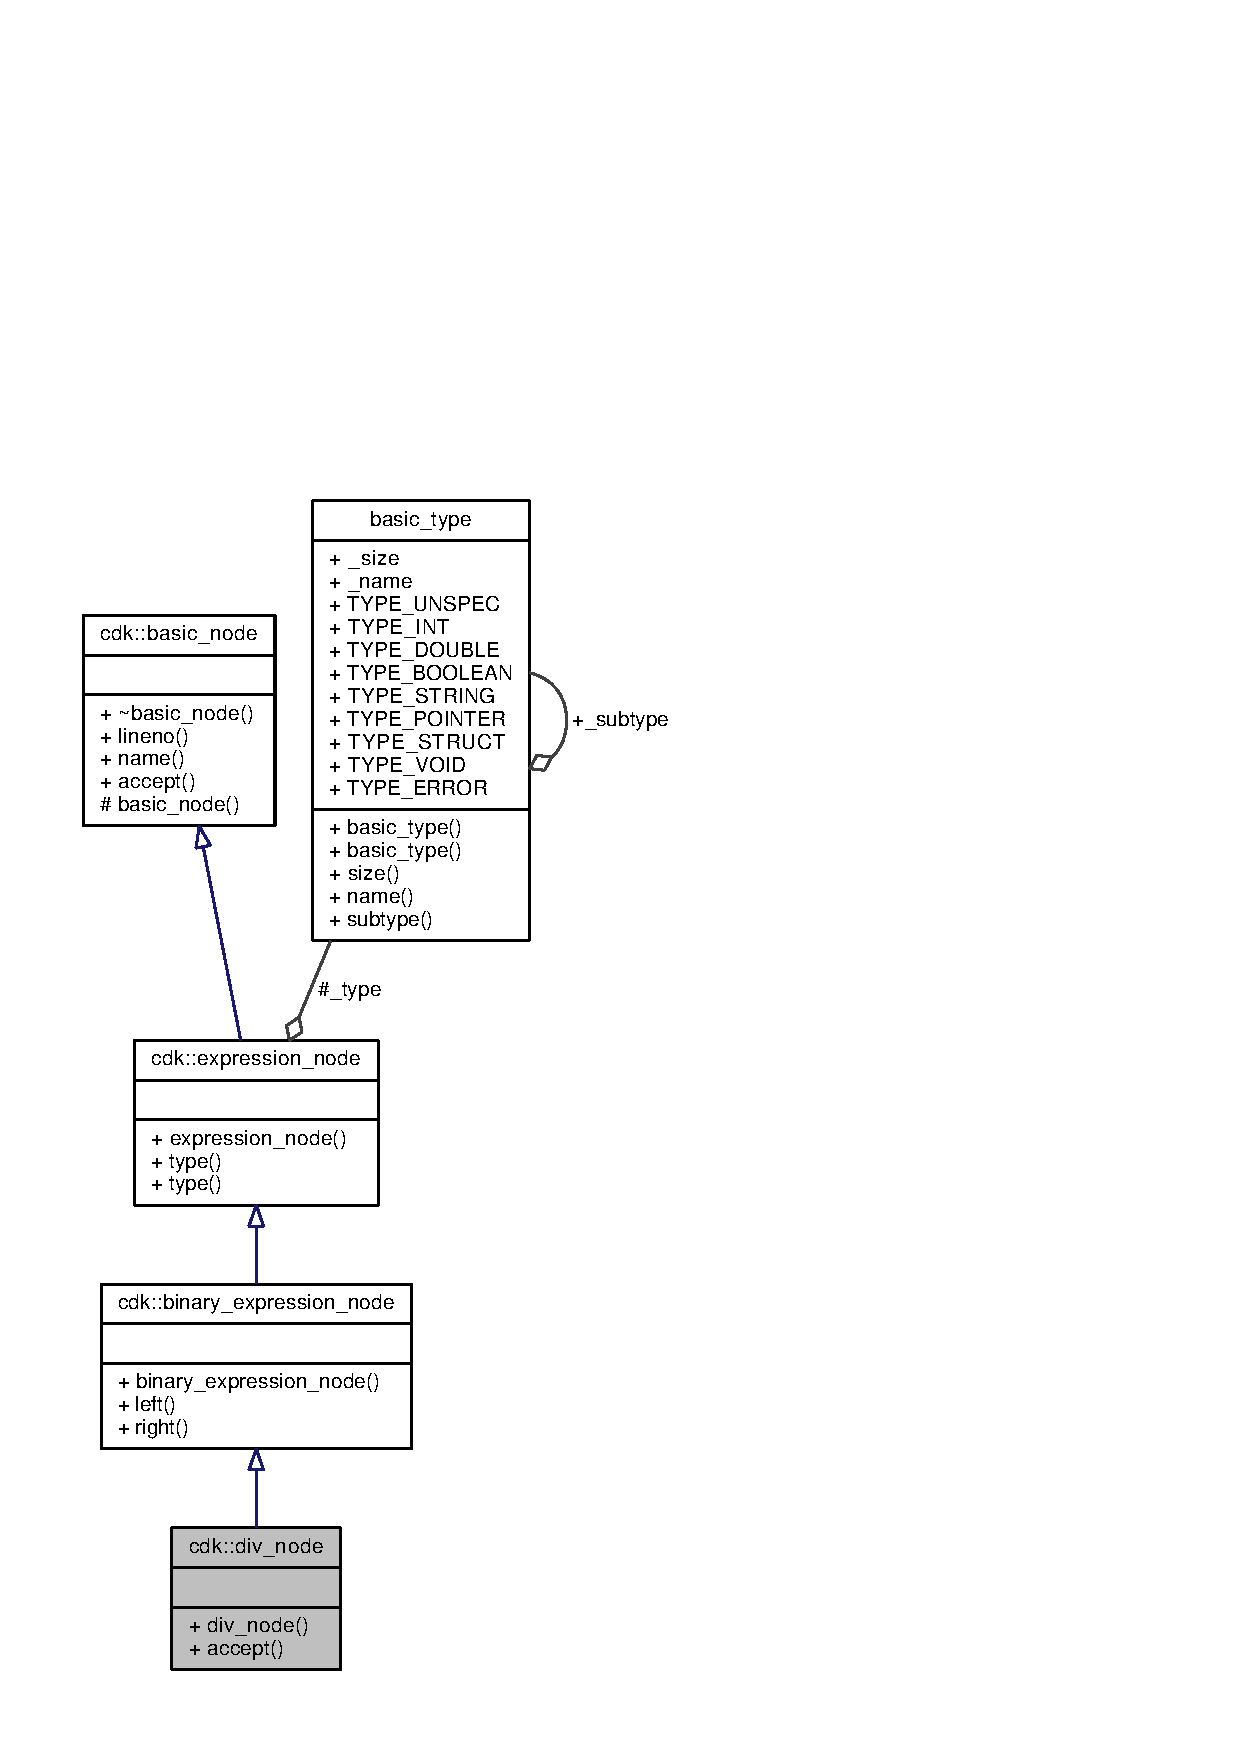
\includegraphics[height=550pt]{classcdk_1_1div__node__coll__graph}
\end{center}
\end{figure}
\subsection*{Public Member Functions}
\begin{DoxyCompactItemize}
\item 
{\bf div\+\_\+node} (int {\bf lineno}, {\bf expression\+\_\+node} $\ast$left, {\bf expression\+\_\+node} $\ast$right)
\item 
void {\bf accept} ({\bf basic\+\_\+ast\+\_\+visitor} $\ast$sp, int level)
\end{DoxyCompactItemize}
\subsection*{Additional Inherited Members}


\subsection{Detailed Description}
Class for describing the division operator 

Definition at line 12 of file div\+\_\+node.\+h.



\subsection{Constructor \& Destructor Documentation}
\index{cdk\+::div\+\_\+node@{cdk\+::div\+\_\+node}!div\+\_\+node@{div\+\_\+node}}
\index{div\+\_\+node@{div\+\_\+node}!cdk\+::div\+\_\+node@{cdk\+::div\+\_\+node}}
\subsubsection[{div\+\_\+node}]{\setlength{\rightskip}{0pt plus 5cm}cdk\+::div\+\_\+node\+::div\+\_\+node (
\begin{DoxyParamCaption}
\item[{int}]{lineno, }
\item[{{\bf expression\+\_\+node} $\ast$}]{left, }
\item[{{\bf expression\+\_\+node} $\ast$}]{right}
\end{DoxyParamCaption}
)\hspace{0.3cm}{\ttfamily [inline]}}\label{classcdk_1_1div__node_ae5883f44a0fd349b2a8994bc209b155c}
\begin{DoxySeeAlso}{See also}
Binary\+Expression 
\end{DoxySeeAlso}


Definition at line 15 of file div\+\_\+node.\+h.



\subsection{Member Function Documentation}
\index{cdk\+::div\+\_\+node@{cdk\+::div\+\_\+node}!accept@{accept}}
\index{accept@{accept}!cdk\+::div\+\_\+node@{cdk\+::div\+\_\+node}}
\subsubsection[{accept}]{\setlength{\rightskip}{0pt plus 5cm}void cdk\+::div\+\_\+node\+::accept (
\begin{DoxyParamCaption}
\item[{{\bf basic\+\_\+ast\+\_\+visitor} $\ast$}]{sp, }
\item[{int}]{level}
\end{DoxyParamCaption}
)\hspace{0.3cm}{\ttfamily [inline]}, {\ttfamily [virtual]}}\label{classcdk_1_1div__node_a18fdb1b825aeba112a607964f3901a6d}

\begin{DoxyParams}{Parameters}
{\em sp} & semantic processor visitor \\
\hline
{\em level} & syntactic tree level \\
\hline
\end{DoxyParams}


Implements {\bf cdk\+::basic\+\_\+node} \doxyref{}{p.}{classcdk_1_1basic__node_ab38adcbc95c46b809961278afae3bf05}.



Definition at line 23 of file div\+\_\+node.\+h.



The documentation for this class was generated from the following file\+:\begin{DoxyCompactItemize}
\item 
ast/div\+\_\+node.\+h\end{DoxyCompactItemize}

\section{cdk\+:\+:double\+\_\+node Class Reference}
\label{classcdk_1_1double__node}\index{cdk\+::double\+\_\+node@{cdk\+::double\+\_\+node}}


{\ttfamily \#include $<$double\+\_\+node.\+h$>$}



Inheritance diagram for cdk\+:\+:double\+\_\+node\+:
\nopagebreak
\begin{figure}[H]
\begin{center}
\leavevmode
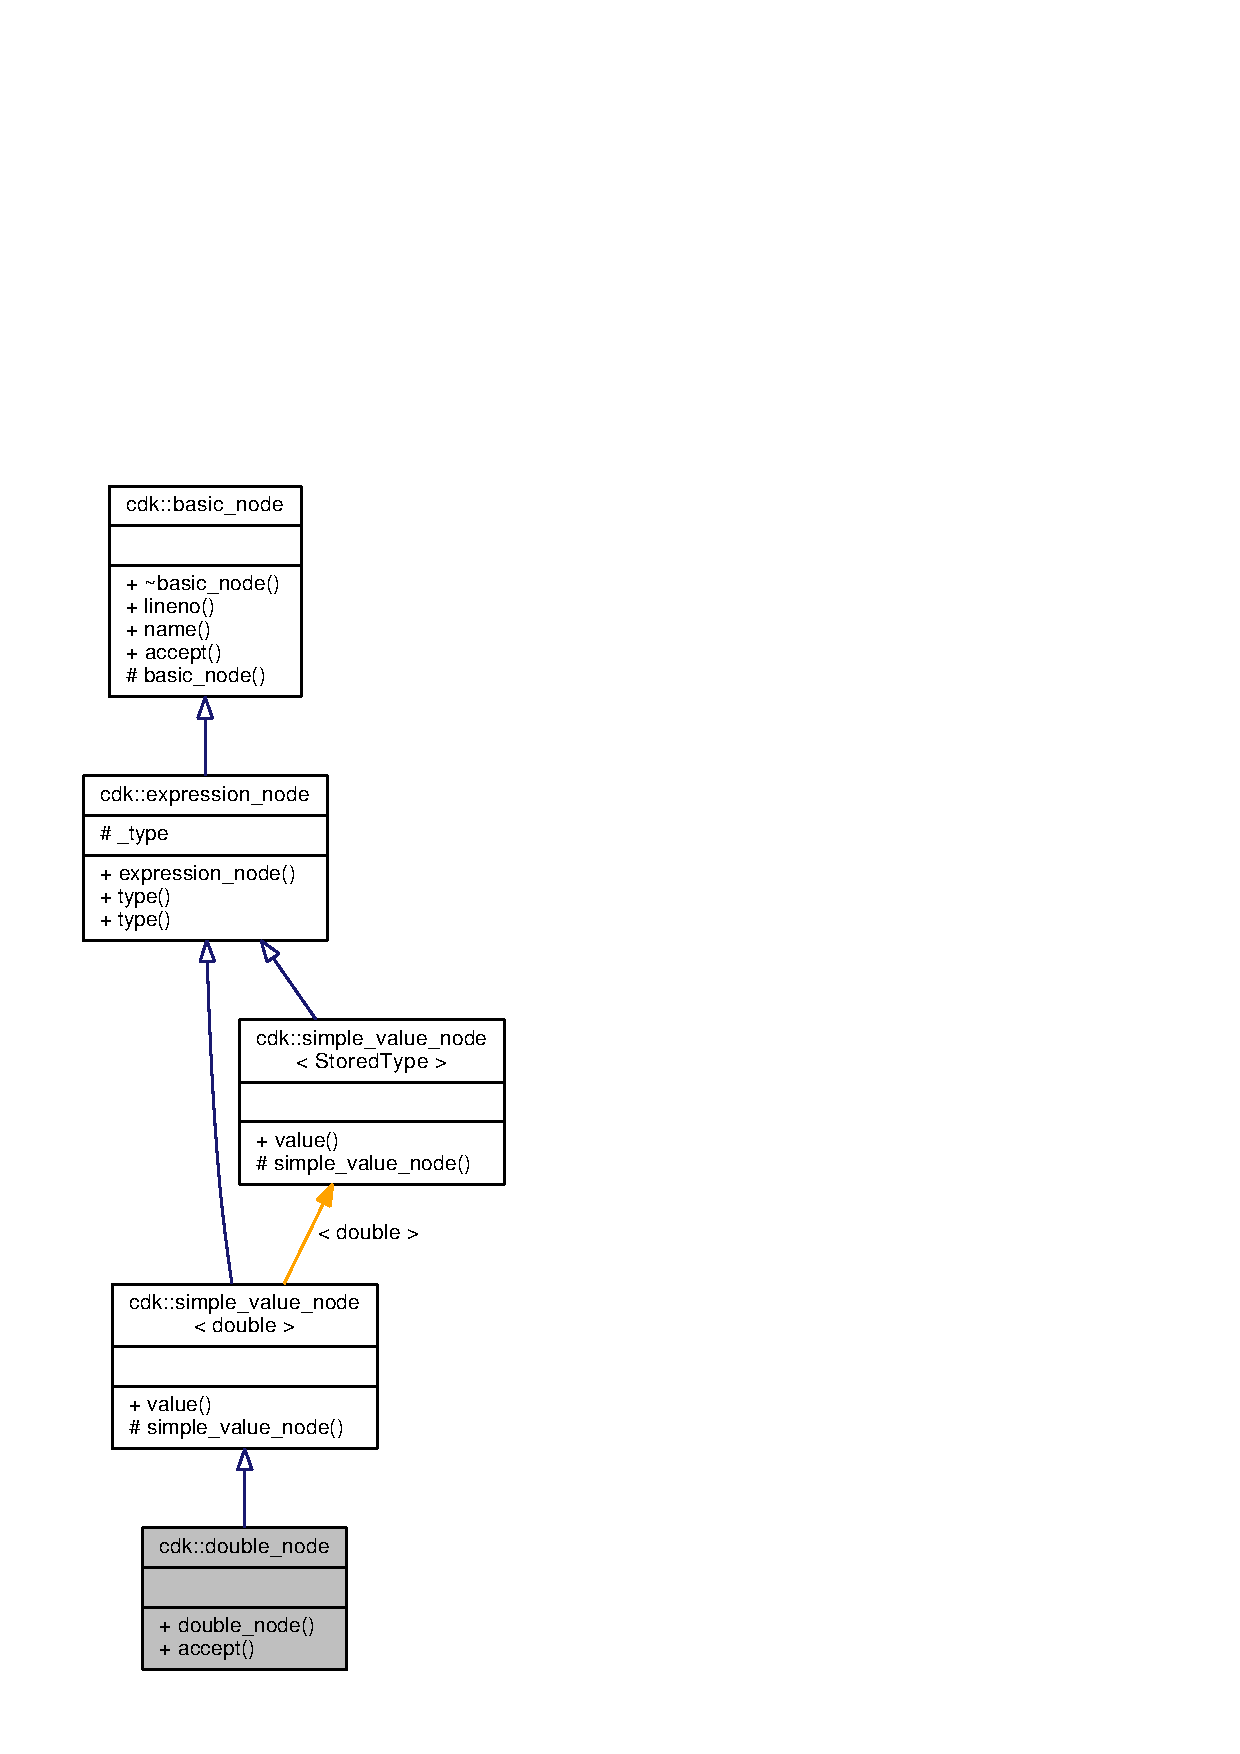
\includegraphics[height=550pt]{classcdk_1_1double__node__inherit__graph}
\end{center}
\end{figure}


Collaboration diagram for cdk\+:\+:double\+\_\+node\+:
\nopagebreak
\begin{figure}[H]
\begin{center}
\leavevmode
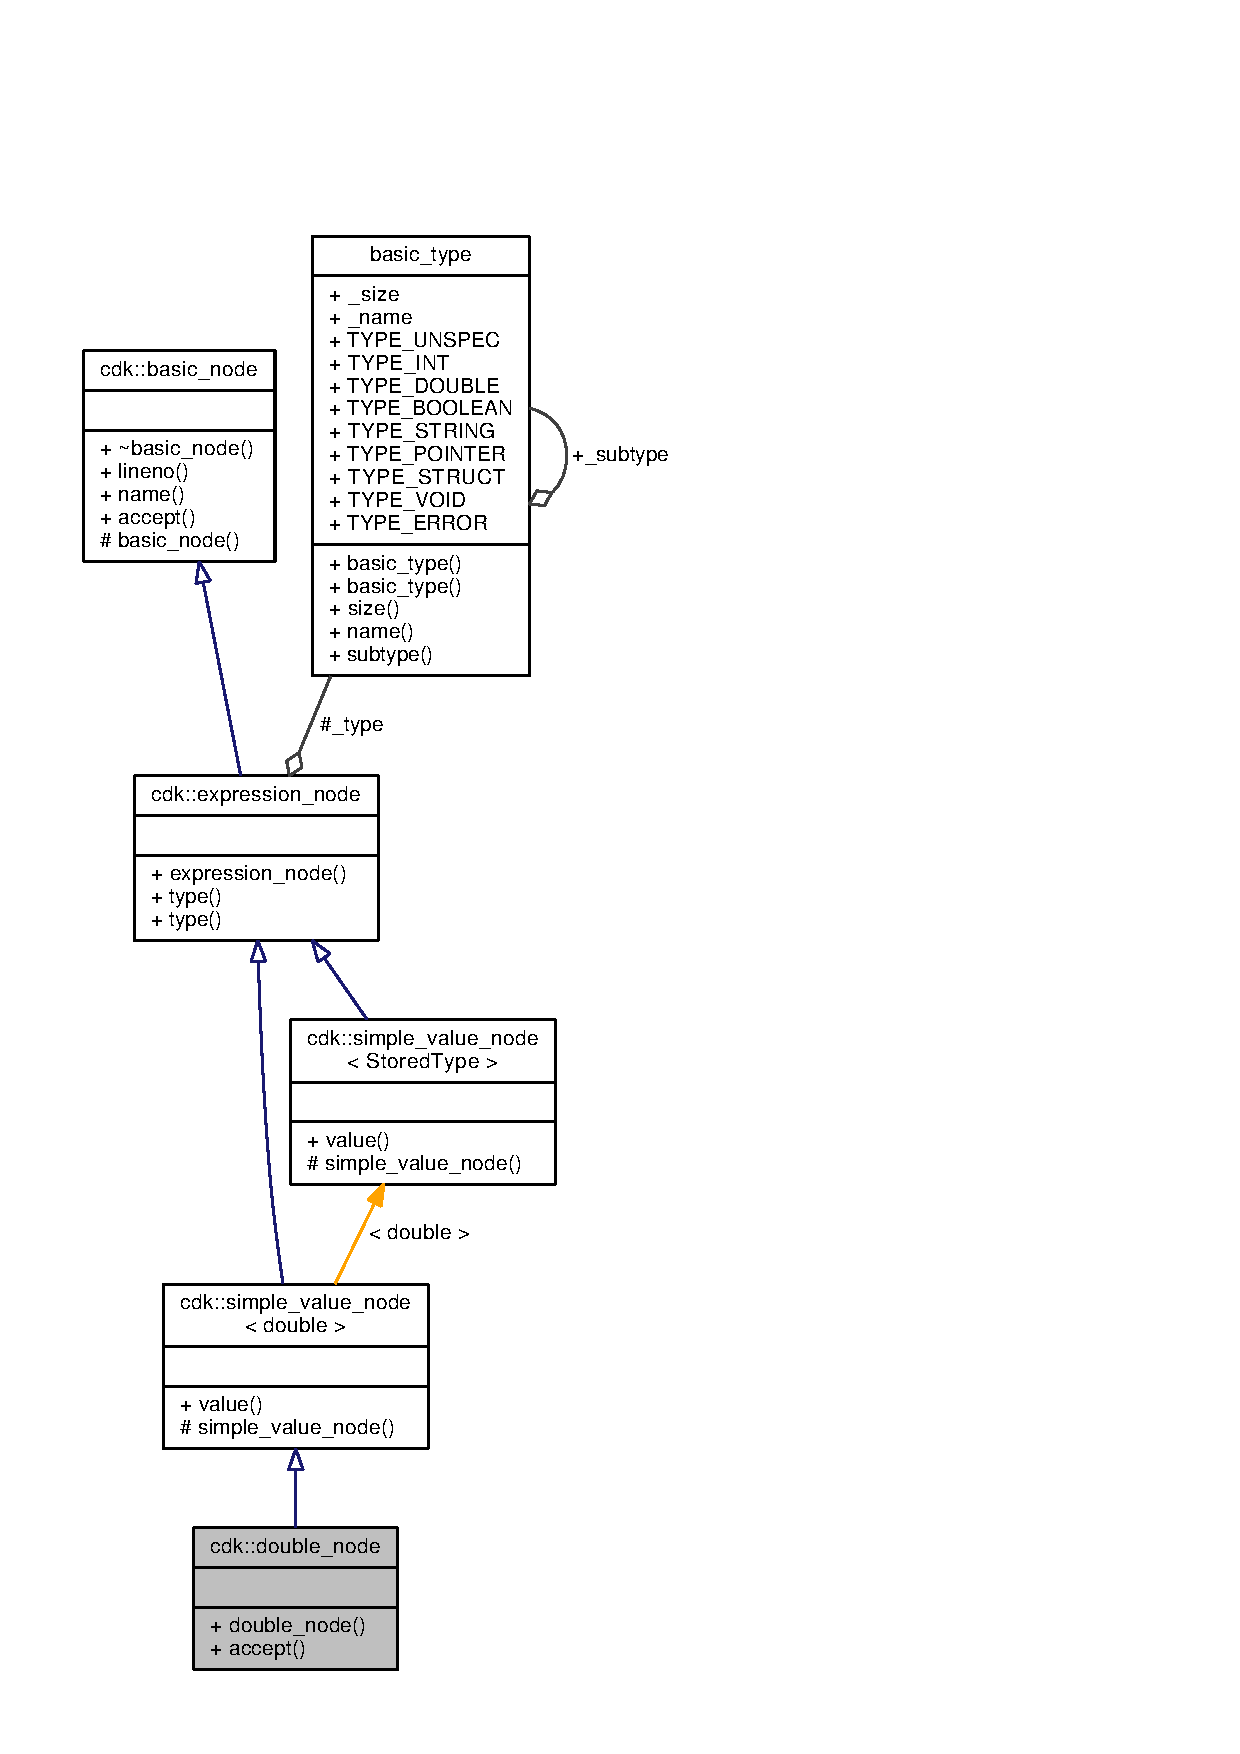
\includegraphics[height=550pt]{classcdk_1_1double__node__coll__graph}
\end{center}
\end{figure}
\subsection*{Public Member Functions}
\begin{DoxyCompactItemize}
\item 
{\bfseries double\+\_\+node} (int {\bf lineno}, double d)\label{classcdk_1_1double__node_aae6671702e1b25b696f7c54fc23a4a99}

\item 
void {\bf accept} ({\bf basic\+\_\+ast\+\_\+visitor} $\ast$sp, int level)
\end{DoxyCompactItemize}
\subsection*{Additional Inherited Members}


\subsection{Detailed Description}
Class for describing syntactic tree leaves for holding double precision values. 

Definition at line 13 of file double\+\_\+node.\+h.



\subsection{Member Function Documentation}
\index{cdk\+::double\+\_\+node@{cdk\+::double\+\_\+node}!accept@{accept}}
\index{accept@{accept}!cdk\+::double\+\_\+node@{cdk\+::double\+\_\+node}}
\subsubsection[{accept}]{\setlength{\rightskip}{0pt plus 5cm}void cdk\+::double\+\_\+node\+::accept (
\begin{DoxyParamCaption}
\item[{{\bf basic\+\_\+ast\+\_\+visitor} $\ast$}]{sp, }
\item[{int}]{level}
\end{DoxyParamCaption}
)\hspace{0.3cm}{\ttfamily [inline]}, {\ttfamily [virtual]}}\label{classcdk_1_1double__node_a3338941e9e94a4f88df4a418092c1ec8}

\begin{DoxyParams}{Parameters}
{\em sp} & semantic processor visitor \\
\hline
{\em level} & syntactic tree level \\
\hline
\end{DoxyParams}


Implements {\bf cdk\+::basic\+\_\+node} \doxyref{}{p.}{classcdk_1_1basic__node_ab38adcbc95c46b809961278afae3bf05}.



Definition at line 23 of file double\+\_\+node.\+h.



The documentation for this class was generated from the following file\+:\begin{DoxyCompactItemize}
\item 
ast/double\+\_\+node.\+h\end{DoxyCompactItemize}

\section{cdk\+:\+:eq\+\_\+node Class Reference}
\label{classcdk_1_1eq__node}\index{cdk\+::eq\+\_\+node@{cdk\+::eq\+\_\+node}}


{\ttfamily \#include $<$eq\+\_\+node.\+h$>$}



Inheritance diagram for cdk\+:\+:eq\+\_\+node\+:
\nopagebreak
\begin{figure}[H]
\begin{center}
\leavevmode
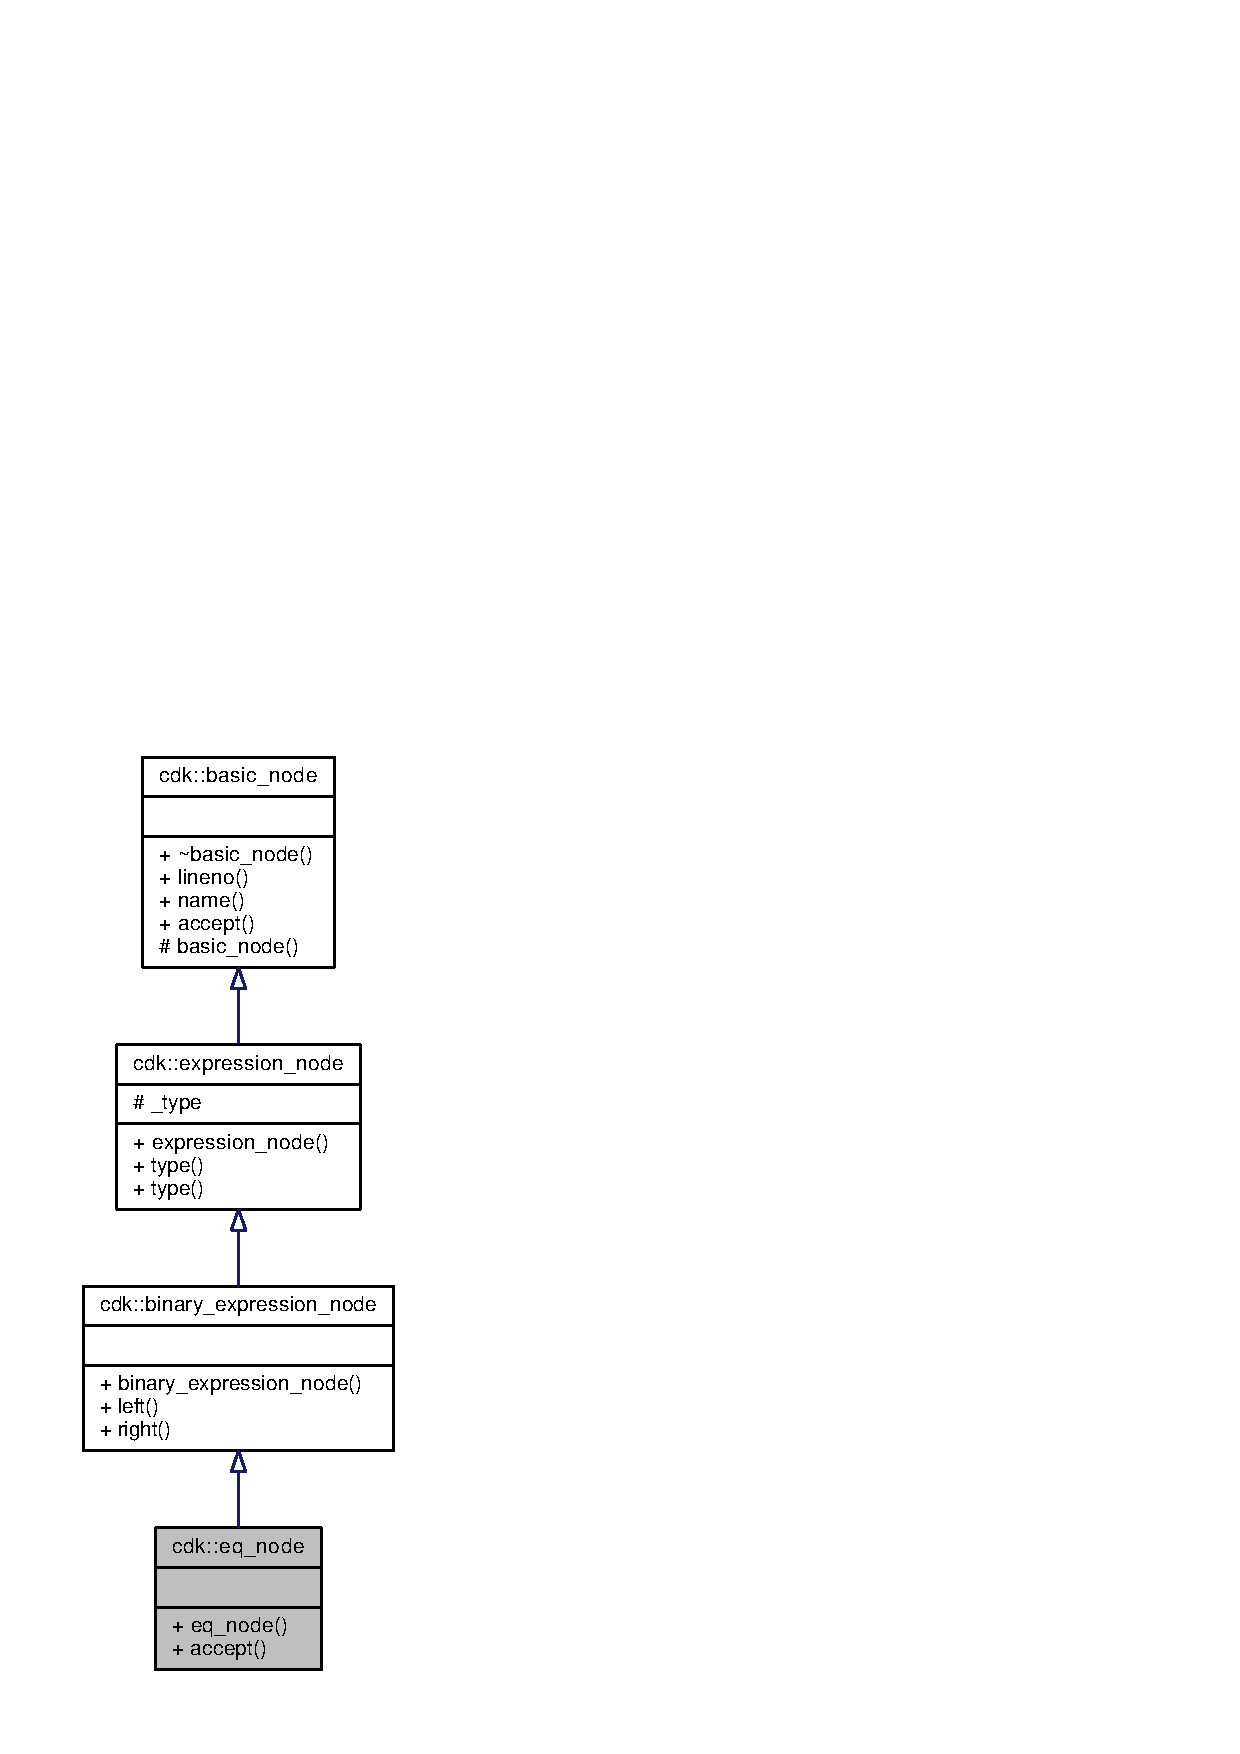
\includegraphics[width=193pt]{classcdk_1_1eq__node__inherit__graph}
\end{center}
\end{figure}


Collaboration diagram for cdk\+:\+:eq\+\_\+node\+:
\nopagebreak
\begin{figure}[H]
\begin{center}
\leavevmode
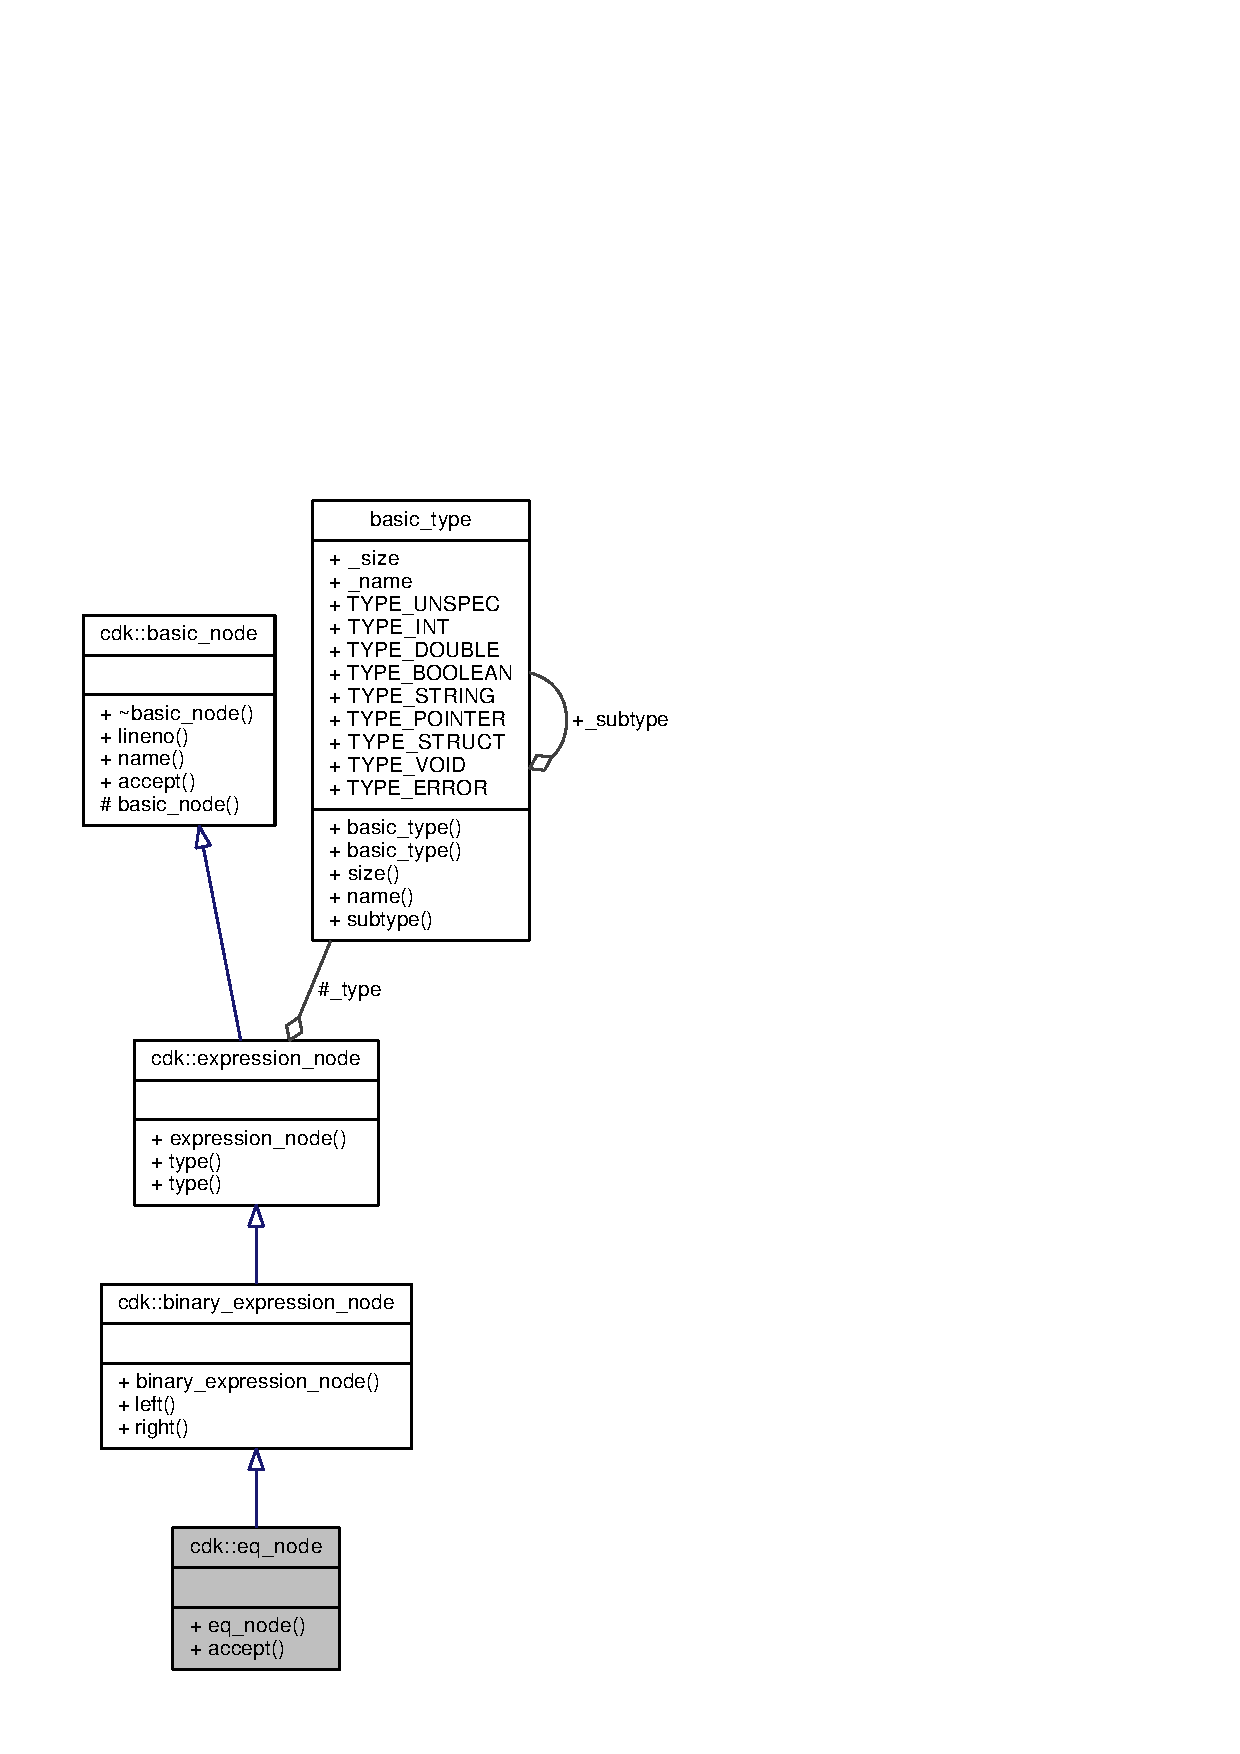
\includegraphics[height=550pt]{classcdk_1_1eq__node__coll__graph}
\end{center}
\end{figure}
\subsection*{Public Member Functions}
\begin{DoxyCompactItemize}
\item 
{\bf eq\+\_\+node} (int {\bf lineno}, {\bf expression\+\_\+node} $\ast$left, {\bf expression\+\_\+node} $\ast$right)
\item 
void {\bf accept} ({\bf basic\+\_\+ast\+\_\+visitor} $\ast$sp, int level)
\end{DoxyCompactItemize}
\subsection*{Additional Inherited Members}


\subsection{Detailed Description}
Class for describing the equality operator 

Definition at line 12 of file eq\+\_\+node.\+h.



\subsection{Constructor \& Destructor Documentation}
\index{cdk\+::eq\+\_\+node@{cdk\+::eq\+\_\+node}!eq\+\_\+node@{eq\+\_\+node}}
\index{eq\+\_\+node@{eq\+\_\+node}!cdk\+::eq\+\_\+node@{cdk\+::eq\+\_\+node}}
\subsubsection[{eq\+\_\+node}]{\setlength{\rightskip}{0pt plus 5cm}cdk\+::eq\+\_\+node\+::eq\+\_\+node (
\begin{DoxyParamCaption}
\item[{int}]{lineno, }
\item[{{\bf expression\+\_\+node} $\ast$}]{left, }
\item[{{\bf expression\+\_\+node} $\ast$}]{right}
\end{DoxyParamCaption}
)\hspace{0.3cm}{\ttfamily [inline]}}\label{classcdk_1_1eq__node_a69cb18aa9ce0d7907192204fe24f4518}

\begin{DoxyParams}{Parameters}
{\em lineno} & source code line number for this node \\
\hline
{\em left} & first operand \\
\hline
{\em right} & second operand \\
\hline
\end{DoxyParams}


Definition at line 20 of file eq\+\_\+node.\+h.



\subsection{Member Function Documentation}
\index{cdk\+::eq\+\_\+node@{cdk\+::eq\+\_\+node}!accept@{accept}}
\index{accept@{accept}!cdk\+::eq\+\_\+node@{cdk\+::eq\+\_\+node}}
\subsubsection[{accept}]{\setlength{\rightskip}{0pt plus 5cm}void cdk\+::eq\+\_\+node\+::accept (
\begin{DoxyParamCaption}
\item[{{\bf basic\+\_\+ast\+\_\+visitor} $\ast$}]{sp, }
\item[{int}]{level}
\end{DoxyParamCaption}
)\hspace{0.3cm}{\ttfamily [inline]}, {\ttfamily [virtual]}}\label{classcdk_1_1eq__node_ac874f2c13fc2f66ce23b08d99594368e}

\begin{DoxyParams}{Parameters}
{\em sp} & semantic processor visitor \\
\hline
{\em level} & syntactic tree level \\
\hline
\end{DoxyParams}


Implements {\bf cdk\+::basic\+\_\+node} \doxyref{}{p.}{classcdk_1_1basic__node_ab38adcbc95c46b809961278afae3bf05}.



Definition at line 28 of file eq\+\_\+node.\+h.



The documentation for this class was generated from the following file\+:\begin{DoxyCompactItemize}
\item 
ast/eq\+\_\+node.\+h\end{DoxyCompactItemize}

\section{cdk\+:\+:expression\+\_\+node Class Reference}
\label{classcdk_1_1expression__node}\index{cdk\+::expression\+\_\+node@{cdk\+::expression\+\_\+node}}


{\ttfamily \#include $<$expression\+\_\+node.\+h$>$}



Inheritance diagram for cdk\+:\+:expression\+\_\+node\+:
\nopagebreak
\begin{figure}[H]
\begin{center}
\leavevmode
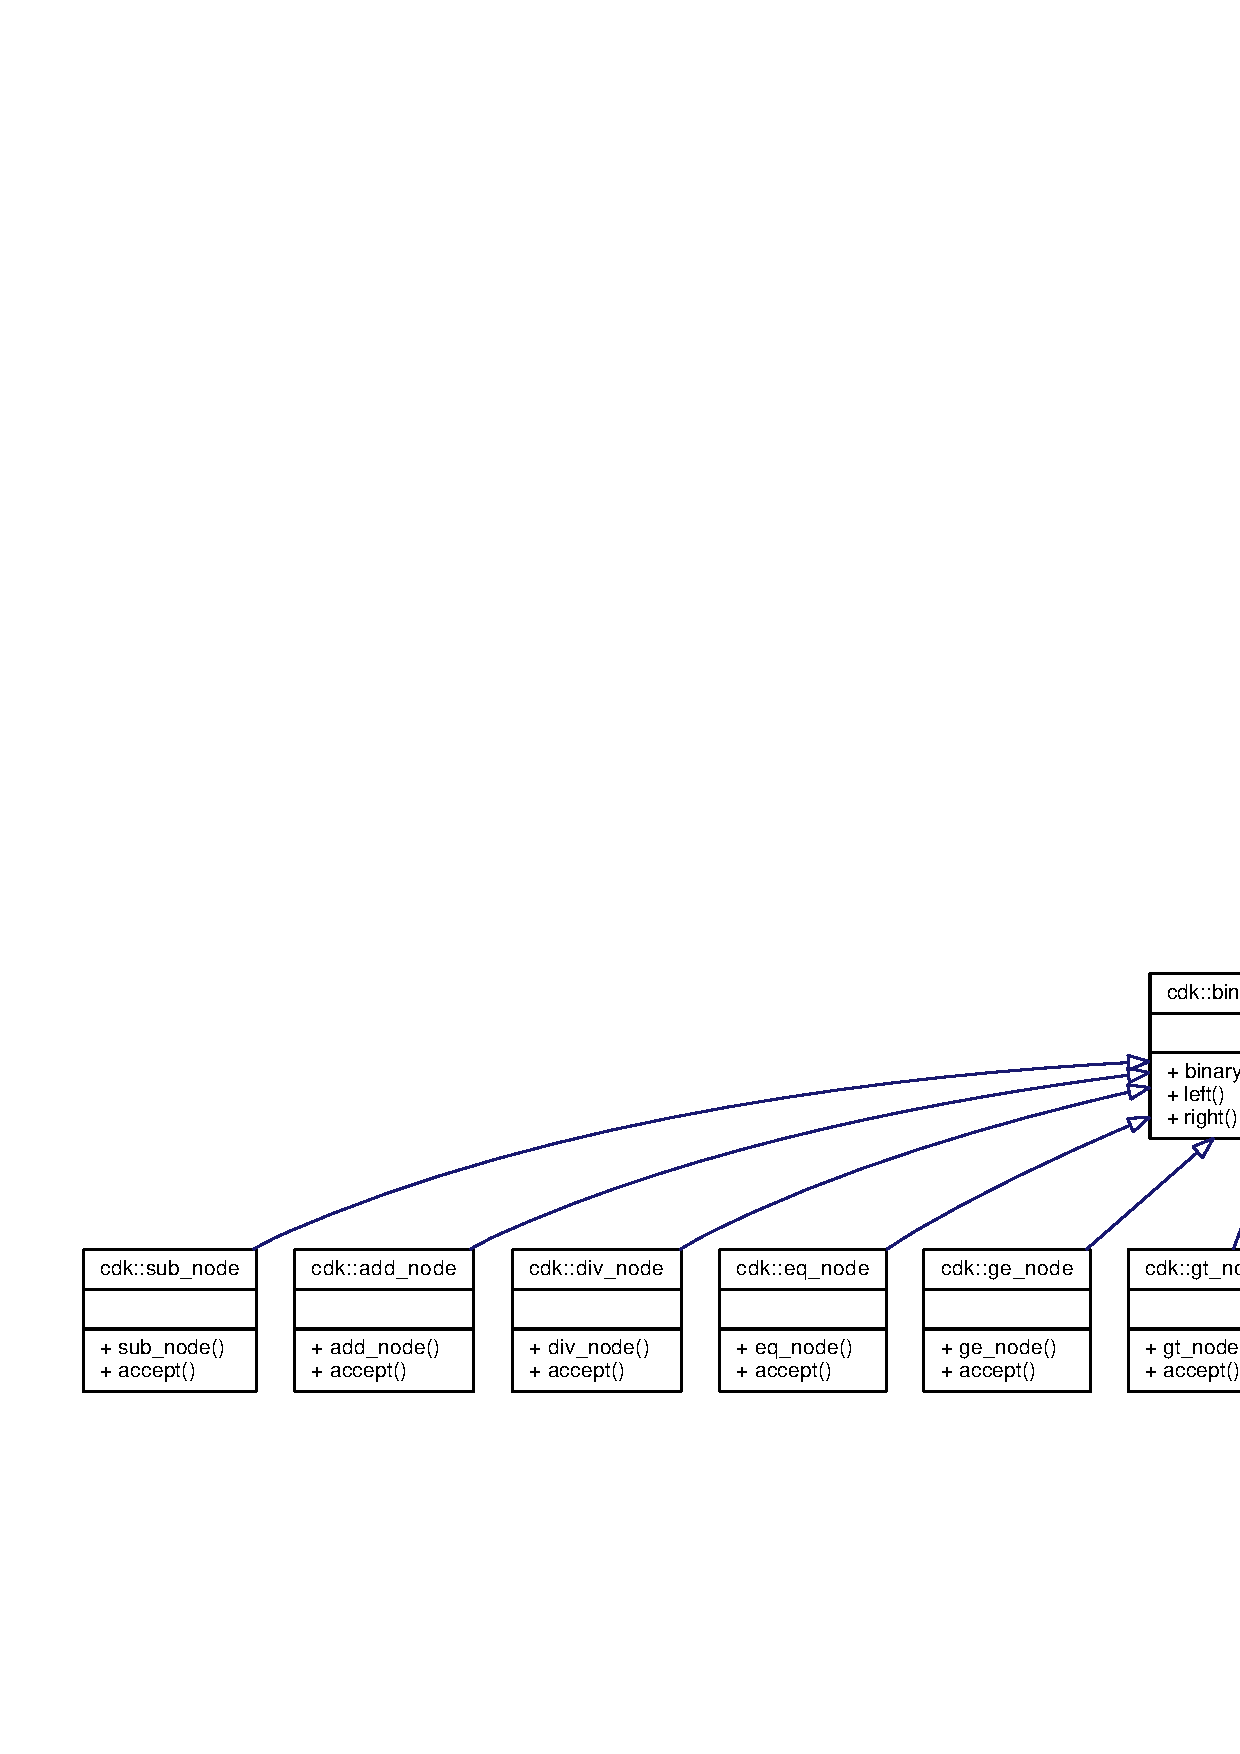
\includegraphics[width=350pt]{classcdk_1_1expression__node__inherit__graph}
\end{center}
\end{figure}


Collaboration diagram for cdk\+:\+:expression\+\_\+node\+:
\nopagebreak
\begin{figure}[H]
\begin{center}
\leavevmode
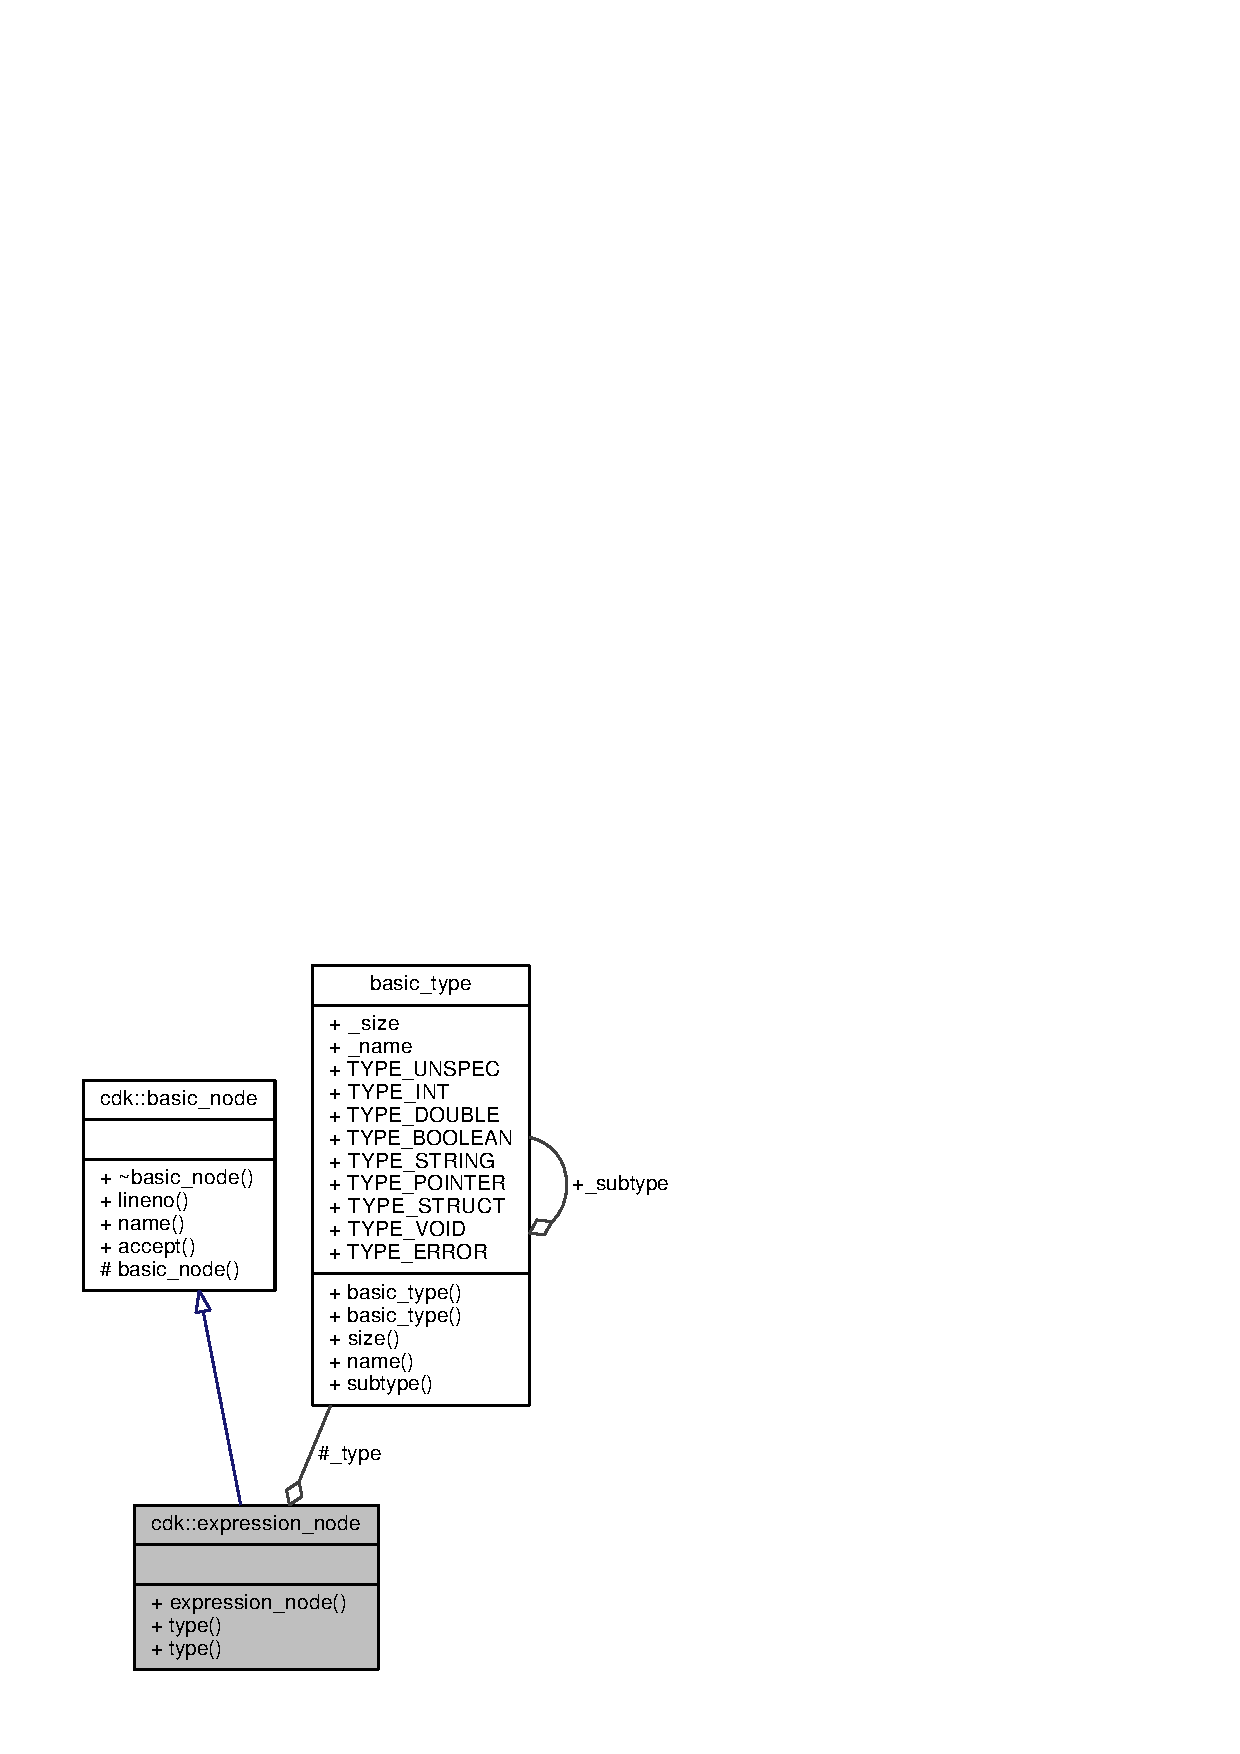
\includegraphics[width=325pt]{classcdk_1_1expression__node__coll__graph}
\end{center}
\end{figure}
\subsection*{Public Member Functions}
\begin{DoxyCompactItemize}
\item 
{\bf expression\+\_\+node} (int {\bf lineno})
\item 
virtual {\bf basic\+\_\+type} $\ast$ {\bfseries type} ()\label{classcdk_1_1expression__node_a1dcde2e24b7eb3544a2cb4814d3d757b}

\item 
virtual void {\bfseries type} ({\bf basic\+\_\+type} $\ast$type)\label{classcdk_1_1expression__node_a56d9027882f84e135d92020149708cb1}

\end{DoxyCompactItemize}
\subsection*{Protected Attributes}
\begin{DoxyCompactItemize}
\item 
{\bf basic\+\_\+type} $\ast$ {\bfseries \+\_\+type}\label{classcdk_1_1expression__node_aee258e43ef6a7f84c83e47eb1524d9f6}

\end{DoxyCompactItemize}
\subsection*{Additional Inherited Members}


\subsection{Detailed Description}
Expressions are typed nodes, i.\+e., able to store a type description. 

Definition at line 14 of file expression\+\_\+node.\+h.



\subsection{Constructor \& Destructor Documentation}
\index{cdk\+::expression\+\_\+node@{cdk\+::expression\+\_\+node}!expression\+\_\+node@{expression\+\_\+node}}
\index{expression\+\_\+node@{expression\+\_\+node}!cdk\+::expression\+\_\+node@{cdk\+::expression\+\_\+node}}
\subsubsection[{expression\+\_\+node}]{\setlength{\rightskip}{0pt plus 5cm}cdk\+::expression\+\_\+node\+::expression\+\_\+node (
\begin{DoxyParamCaption}
\item[{int}]{lineno}
\end{DoxyParamCaption}
)\hspace{0.3cm}{\ttfamily [inline]}}\label{classcdk_1_1expression__node_a026555785146a09f2d53d56e1bb1e984}
Simple constructor.


\begin{DoxyParams}{Parameters}
{\em lineno} & the source code line number corresponding to the node \\
\hline
\end{DoxyParams}


Definition at line 27 of file expression\+\_\+node.\+h.



The documentation for this class was generated from the following file\+:\begin{DoxyCompactItemize}
\item 
ast/expression\+\_\+node.\+h\end{DoxyCompactItemize}

\section{cdk\+:\+:ge\+\_\+node Class Reference}
\label{classcdk_1_1ge__node}\index{cdk\+::ge\+\_\+node@{cdk\+::ge\+\_\+node}}


{\ttfamily \#include $<$ge\+\_\+node.\+h$>$}



Inheritance diagram for cdk\+:\+:ge\+\_\+node\+:
\nopagebreak
\begin{figure}[H]
\begin{center}
\leavevmode
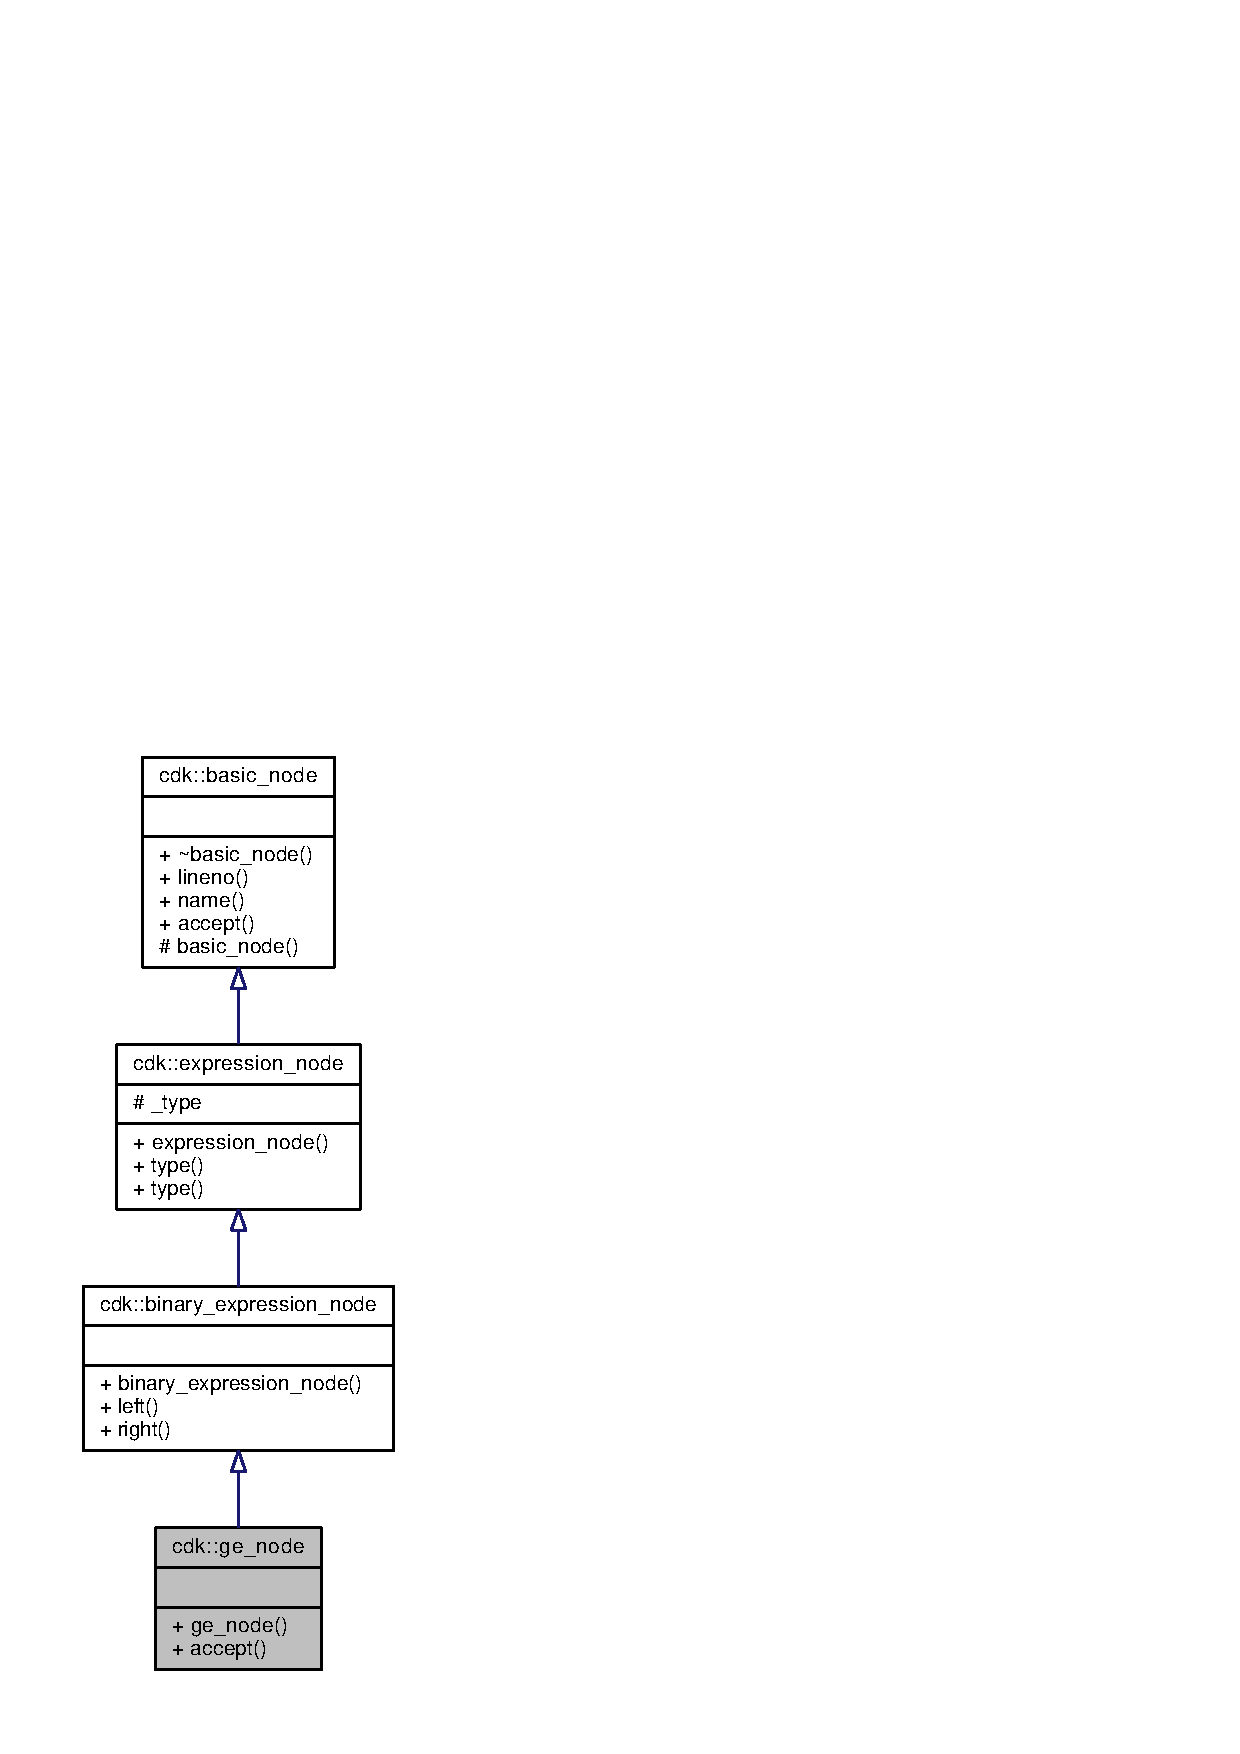
\includegraphics[width=193pt]{classcdk_1_1ge__node__inherit__graph}
\end{center}
\end{figure}


Collaboration diagram for cdk\+:\+:ge\+\_\+node\+:
\nopagebreak
\begin{figure}[H]
\begin{center}
\leavevmode
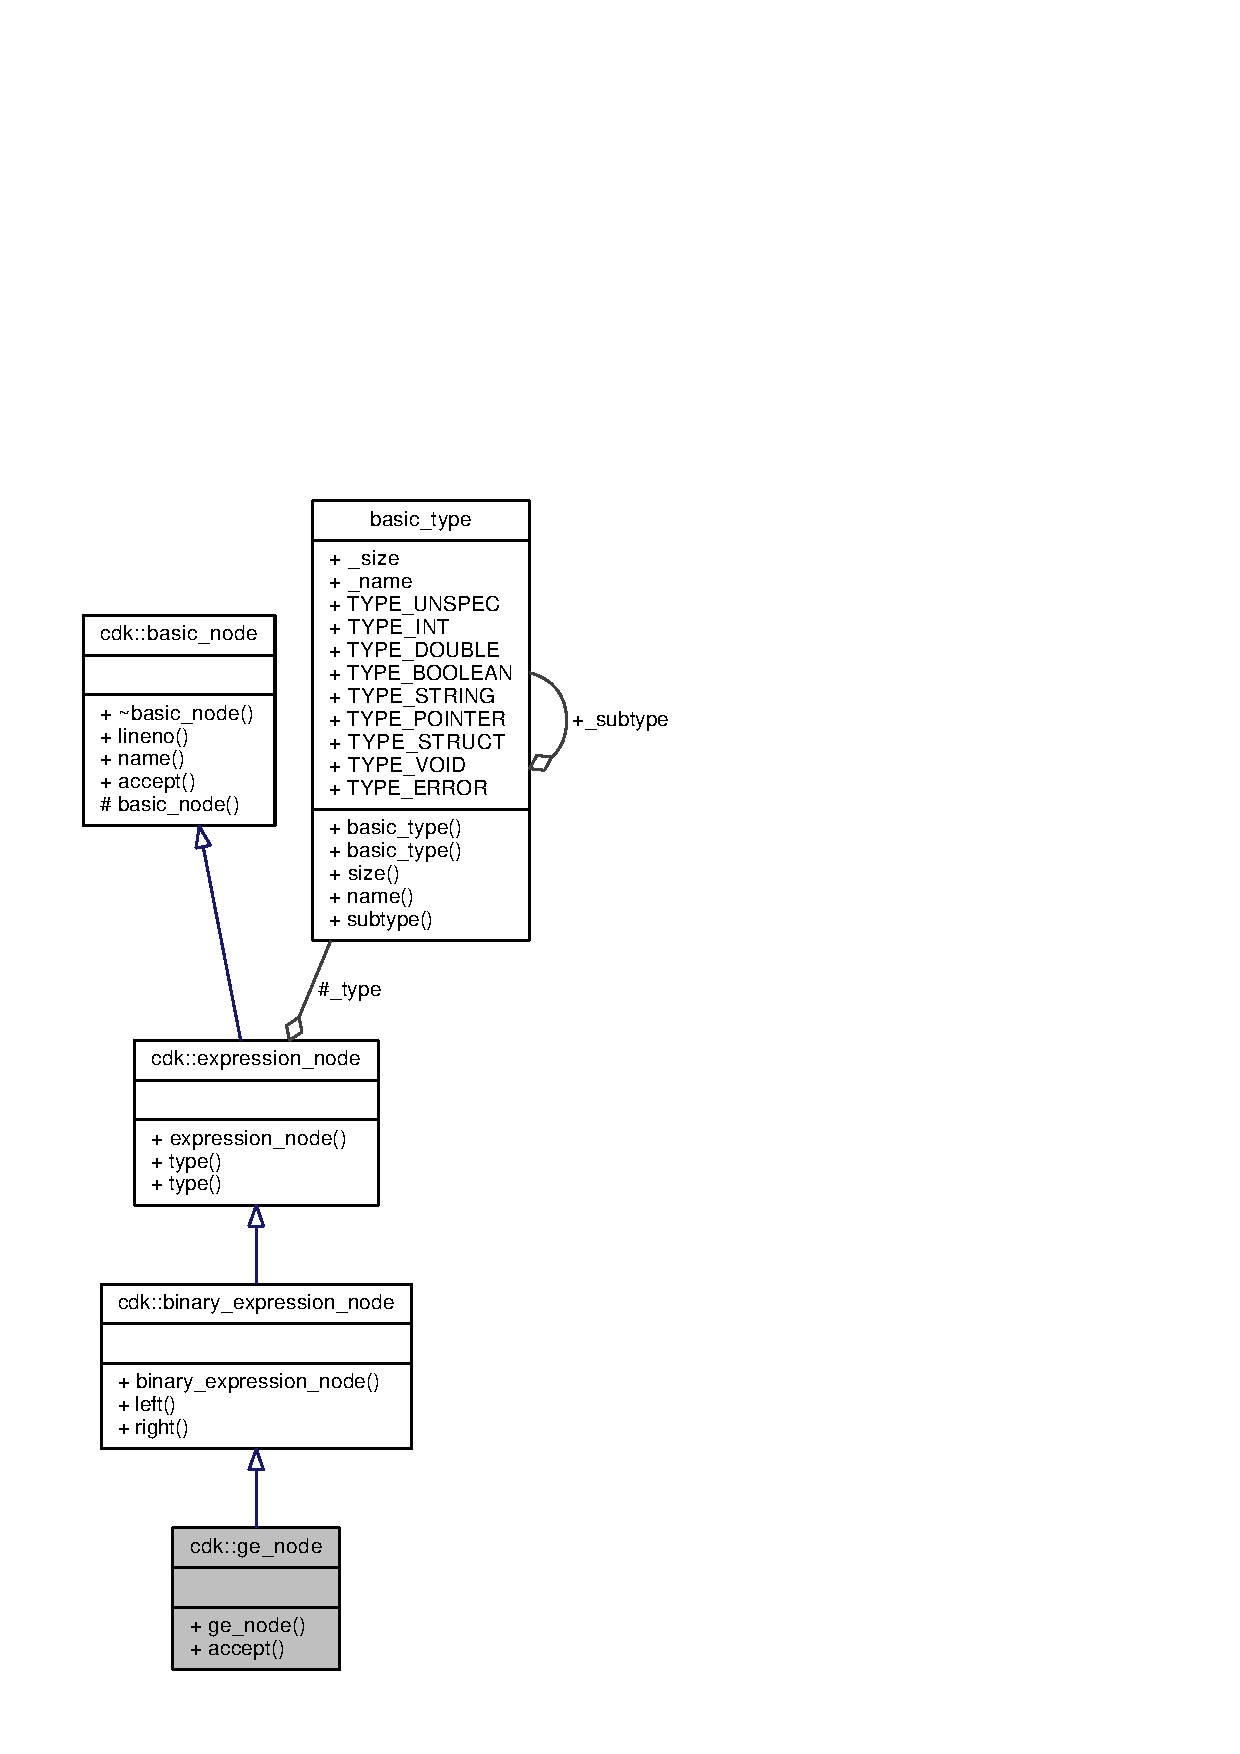
\includegraphics[height=550pt]{classcdk_1_1ge__node__coll__graph}
\end{center}
\end{figure}
\subsection*{Public Member Functions}
\begin{DoxyCompactItemize}
\item 
{\bf ge\+\_\+node} (int {\bf lineno}, {\bf expression\+\_\+node} $\ast$left, {\bf expression\+\_\+node} $\ast$right)
\item 
void {\bf accept} ({\bf basic\+\_\+ast\+\_\+visitor} $\ast$sp, int level)
\end{DoxyCompactItemize}
\subsection*{Additional Inherited Members}


\subsection{Detailed Description}
Class for describing the greater-\/than-\/or-\/equal operator 

Definition at line 12 of file ge\+\_\+node.\+h.



\subsection{Constructor \& Destructor Documentation}
\index{cdk\+::ge\+\_\+node@{cdk\+::ge\+\_\+node}!ge\+\_\+node@{ge\+\_\+node}}
\index{ge\+\_\+node@{ge\+\_\+node}!cdk\+::ge\+\_\+node@{cdk\+::ge\+\_\+node}}
\subsubsection[{ge\+\_\+node}]{\setlength{\rightskip}{0pt plus 5cm}cdk\+::ge\+\_\+node\+::ge\+\_\+node (
\begin{DoxyParamCaption}
\item[{int}]{lineno, }
\item[{{\bf expression\+\_\+node} $\ast$}]{left, }
\item[{{\bf expression\+\_\+node} $\ast$}]{right}
\end{DoxyParamCaption}
)\hspace{0.3cm}{\ttfamily [inline]}}\label{classcdk_1_1ge__node_a41b006478853b8f128a381d136a9055f}

\begin{DoxyParams}{Parameters}
{\em lineno} & source code line number for this node \\
\hline
{\em left} & first operand \\
\hline
{\em right} & second operand \\
\hline
\end{DoxyParams}


Definition at line 19 of file ge\+\_\+node.\+h.



\subsection{Member Function Documentation}
\index{cdk\+::ge\+\_\+node@{cdk\+::ge\+\_\+node}!accept@{accept}}
\index{accept@{accept}!cdk\+::ge\+\_\+node@{cdk\+::ge\+\_\+node}}
\subsubsection[{accept}]{\setlength{\rightskip}{0pt plus 5cm}void cdk\+::ge\+\_\+node\+::accept (
\begin{DoxyParamCaption}
\item[{{\bf basic\+\_\+ast\+\_\+visitor} $\ast$}]{sp, }
\item[{int}]{level}
\end{DoxyParamCaption}
)\hspace{0.3cm}{\ttfamily [inline]}, {\ttfamily [virtual]}}\label{classcdk_1_1ge__node_a758ad0281c1e925aab356d757bedce40}

\begin{DoxyParams}{Parameters}
{\em sp} & semantic processor visitor \\
\hline
{\em level} & syntactic tree level \\
\hline
\end{DoxyParams}


Implements {\bf cdk\+::basic\+\_\+node} \doxyref{}{p.}{classcdk_1_1basic__node_ab38adcbc95c46b809961278afae3bf05}.



Definition at line 27 of file ge\+\_\+node.\+h.



The documentation for this class was generated from the following file\+:\begin{DoxyCompactItemize}
\item 
ast/ge\+\_\+node.\+h\end{DoxyCompactItemize}

\section{cdk\+:\+:gt\+\_\+node Class Reference}
\label{classcdk_1_1gt__node}\index{cdk\+::gt\+\_\+node@{cdk\+::gt\+\_\+node}}


{\ttfamily \#include $<$gt\+\_\+node.\+h$>$}



Inheritance diagram for cdk\+:\+:gt\+\_\+node\+:
\nopagebreak
\begin{figure}[H]
\begin{center}
\leavevmode
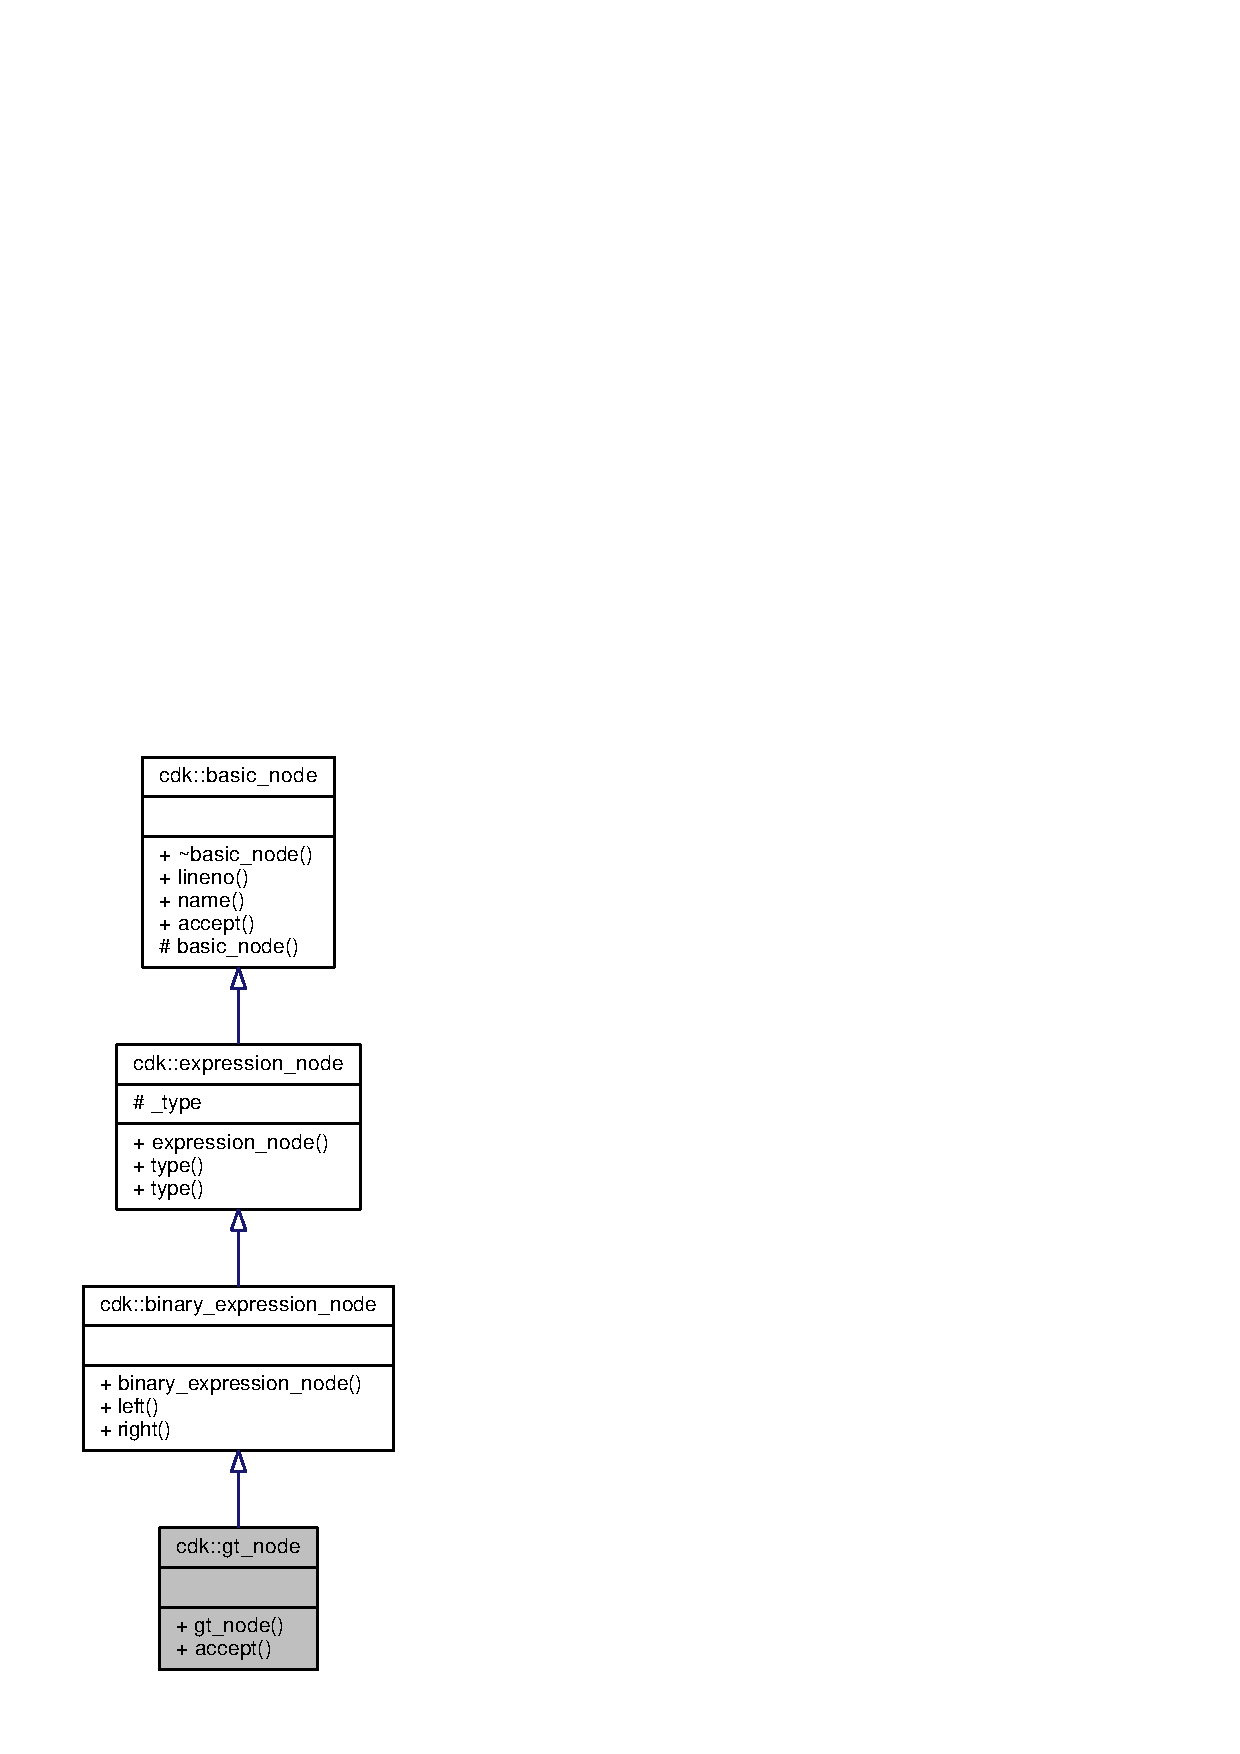
\includegraphics[width=193pt]{classcdk_1_1gt__node__inherit__graph}
\end{center}
\end{figure}


Collaboration diagram for cdk\+:\+:gt\+\_\+node\+:
\nopagebreak
\begin{figure}[H]
\begin{center}
\leavevmode
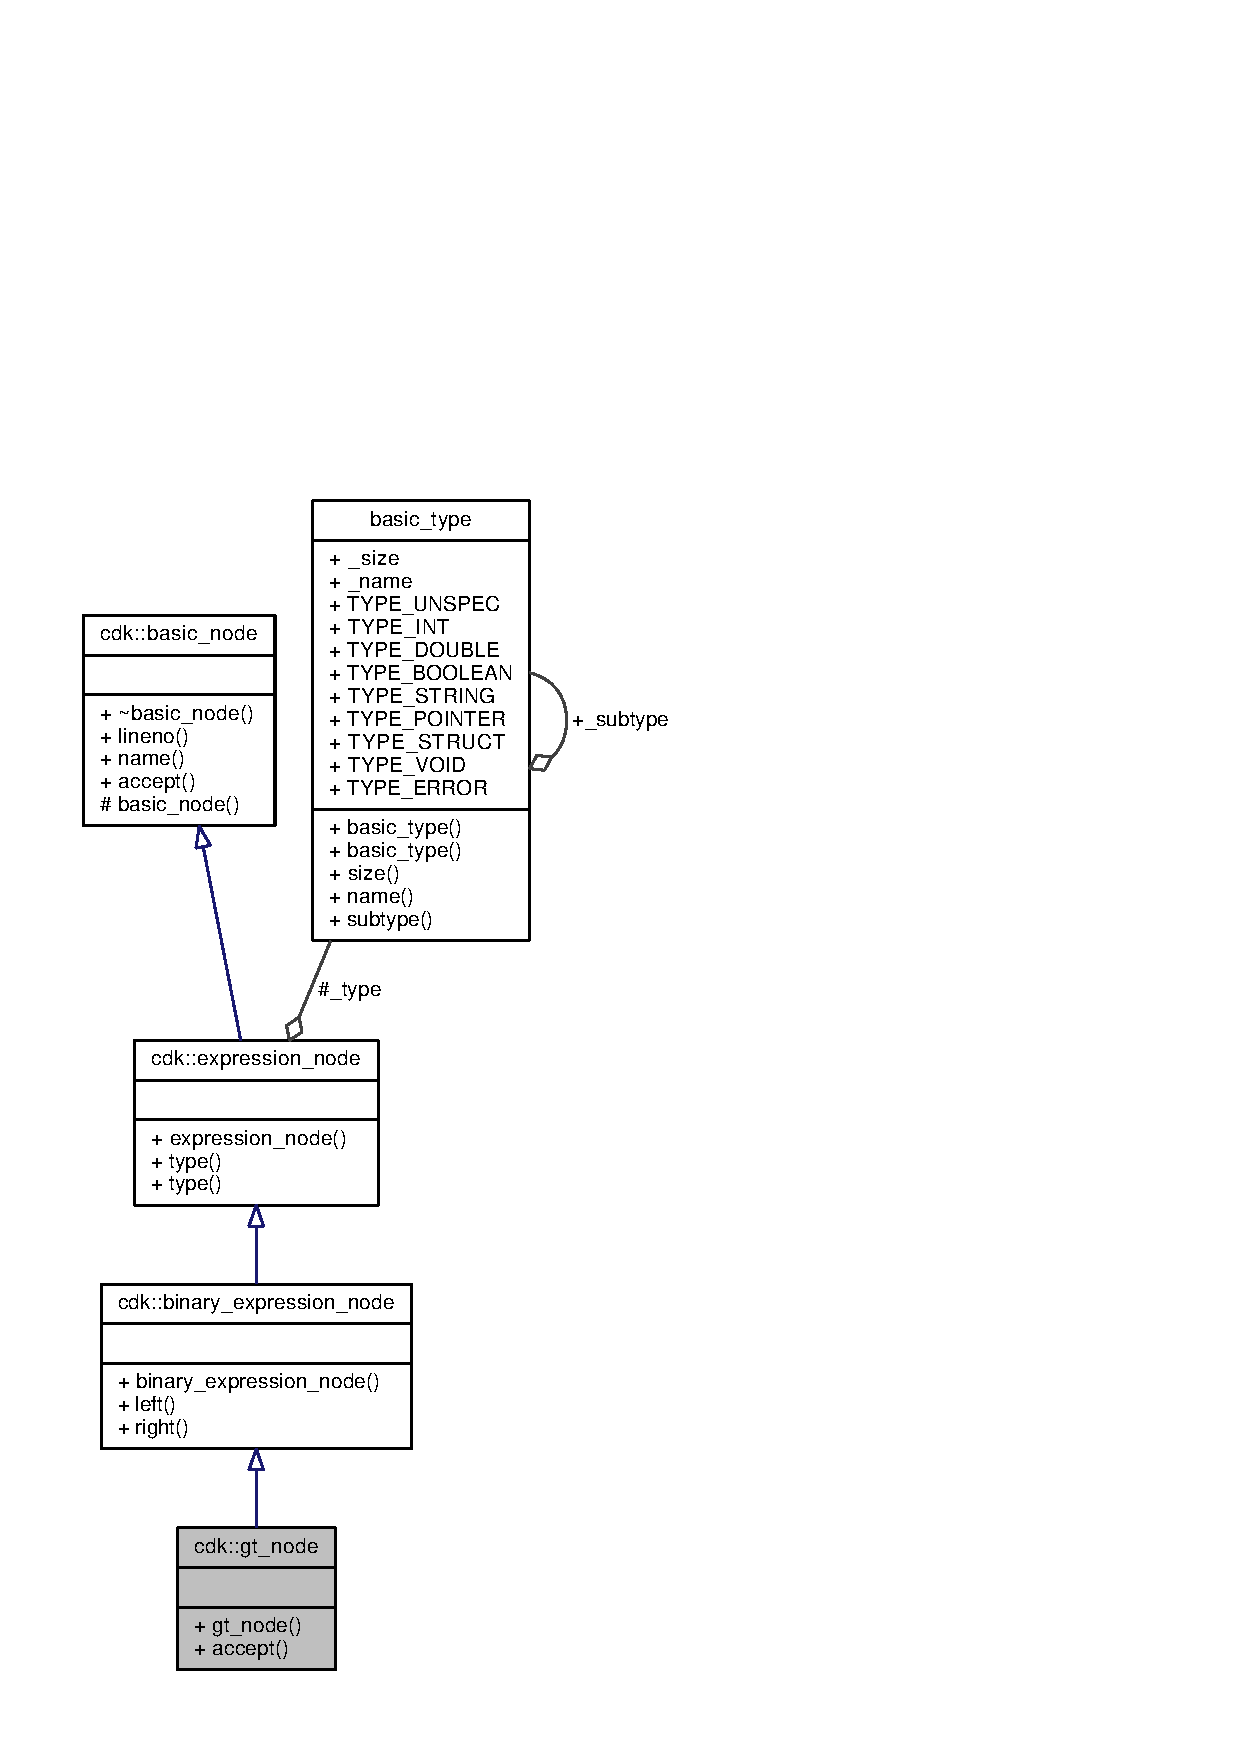
\includegraphics[height=550pt]{classcdk_1_1gt__node__coll__graph}
\end{center}
\end{figure}
\subsection*{Public Member Functions}
\begin{DoxyCompactItemize}
\item 
{\bf gt\+\_\+node} (int {\bf lineno}, {\bf expression\+\_\+node} $\ast$left, {\bf expression\+\_\+node} $\ast$right)
\item 
void {\bf accept} ({\bf basic\+\_\+ast\+\_\+visitor} $\ast$sp, int level)
\end{DoxyCompactItemize}
\subsection*{Additional Inherited Members}


\subsection{Detailed Description}
Class for describing the greater-\/than operator 

Definition at line 12 of file gt\+\_\+node.\+h.



\subsection{Constructor \& Destructor Documentation}
\index{cdk\+::gt\+\_\+node@{cdk\+::gt\+\_\+node}!gt\+\_\+node@{gt\+\_\+node}}
\index{gt\+\_\+node@{gt\+\_\+node}!cdk\+::gt\+\_\+node@{cdk\+::gt\+\_\+node}}
\subsubsection[{gt\+\_\+node}]{\setlength{\rightskip}{0pt plus 5cm}cdk\+::gt\+\_\+node\+::gt\+\_\+node (
\begin{DoxyParamCaption}
\item[{int}]{lineno, }
\item[{{\bf expression\+\_\+node} $\ast$}]{left, }
\item[{{\bf expression\+\_\+node} $\ast$}]{right}
\end{DoxyParamCaption}
)\hspace{0.3cm}{\ttfamily [inline]}}\label{classcdk_1_1gt__node_addd29c7a03ecba8714dbb097c856dfd9}

\begin{DoxyParams}{Parameters}
{\em lineno} & source code line number for this node \\
\hline
{\em left} & first operand \\
\hline
{\em right} & second operand \\
\hline
\end{DoxyParams}


Definition at line 19 of file gt\+\_\+node.\+h.



\subsection{Member Function Documentation}
\index{cdk\+::gt\+\_\+node@{cdk\+::gt\+\_\+node}!accept@{accept}}
\index{accept@{accept}!cdk\+::gt\+\_\+node@{cdk\+::gt\+\_\+node}}
\subsubsection[{accept}]{\setlength{\rightskip}{0pt plus 5cm}void cdk\+::gt\+\_\+node\+::accept (
\begin{DoxyParamCaption}
\item[{{\bf basic\+\_\+ast\+\_\+visitor} $\ast$}]{sp, }
\item[{int}]{level}
\end{DoxyParamCaption}
)\hspace{0.3cm}{\ttfamily [inline]}, {\ttfamily [virtual]}}\label{classcdk_1_1gt__node_ab1104710ad583f4b13d397bf33b2f9f5}

\begin{DoxyParams}{Parameters}
{\em sp} & semantic processor visitor \\
\hline
{\em level} & syntactic tree level \\
\hline
\end{DoxyParams}


Implements {\bf cdk\+::basic\+\_\+node} \doxyref{}{p.}{classcdk_1_1basic__node_ab38adcbc95c46b809961278afae3bf05}.



Definition at line 27 of file gt\+\_\+node.\+h.



The documentation for this class was generated from the following file\+:\begin{DoxyCompactItemize}
\item 
ast/gt\+\_\+node.\+h\end{DoxyCompactItemize}

\section{cdk\+:\+:identifier\+\_\+node Class Reference}
\label{classcdk_1_1identifier__node}\index{cdk\+::identifier\+\_\+node@{cdk\+::identifier\+\_\+node}}


{\ttfamily \#include $<$identifier\+\_\+node.\+h$>$}



Inheritance diagram for cdk\+:\+:identifier\+\_\+node\+:
\nopagebreak
\begin{figure}[H]
\begin{center}
\leavevmode
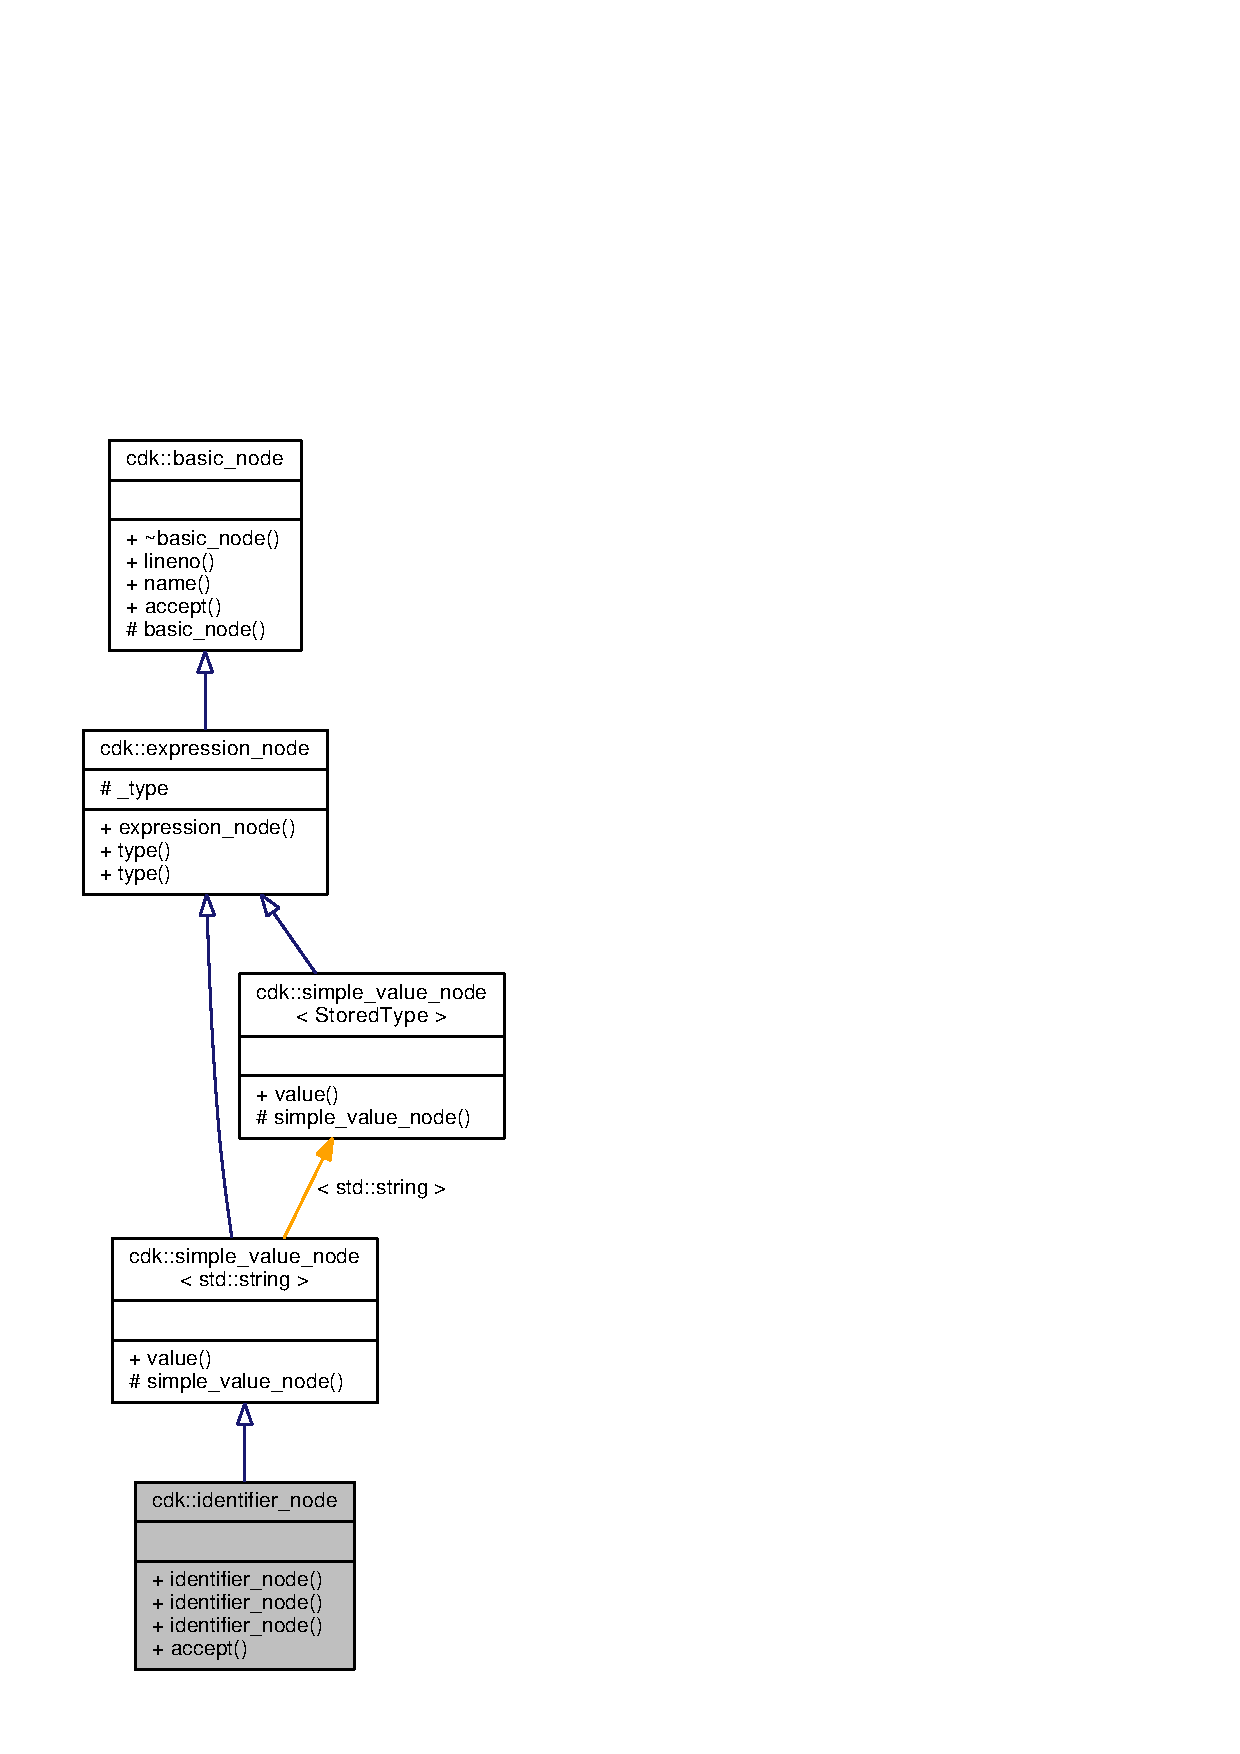
\includegraphics[height=550pt]{classcdk_1_1identifier__node__inherit__graph}
\end{center}
\end{figure}


Collaboration diagram for cdk\+:\+:identifier\+\_\+node\+:
\nopagebreak
\begin{figure}[H]
\begin{center}
\leavevmode
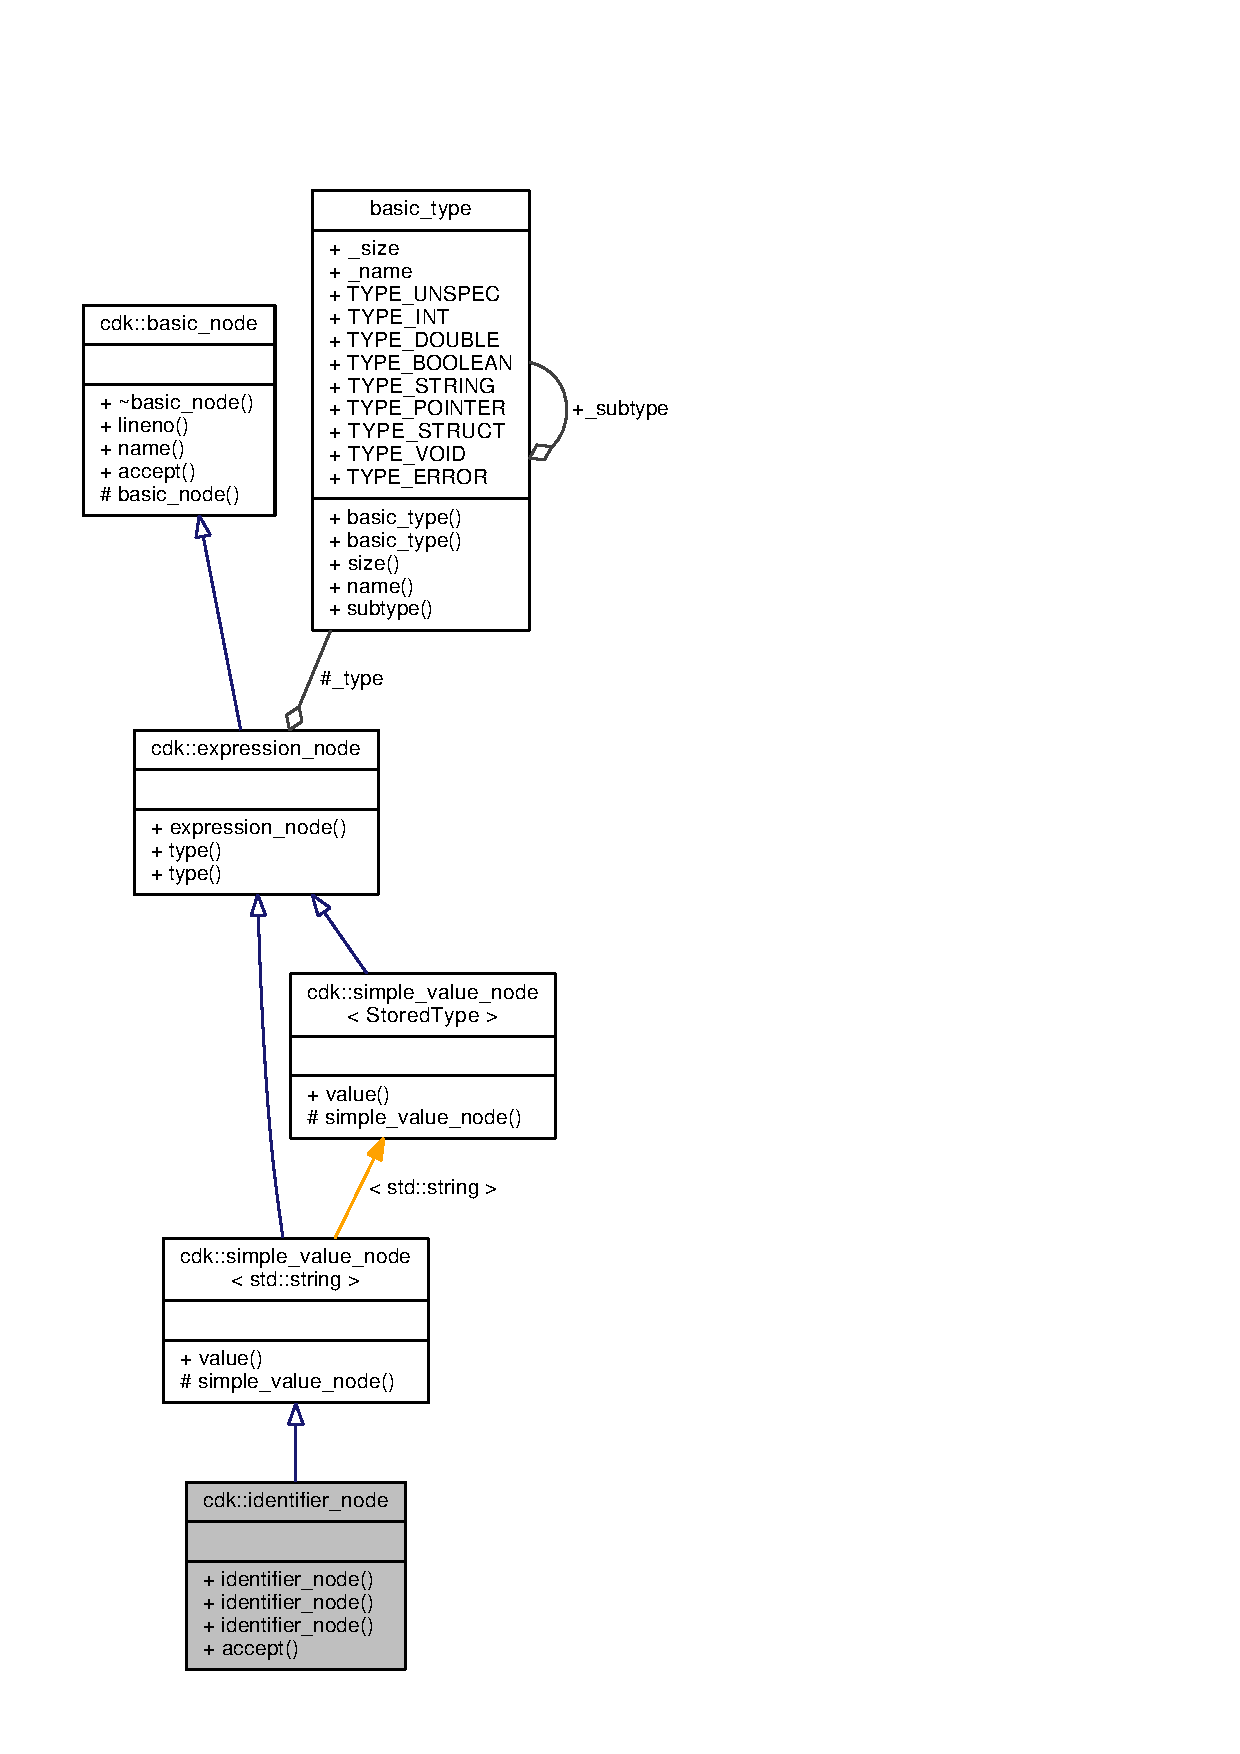
\includegraphics[height=550pt]{classcdk_1_1identifier__node__coll__graph}
\end{center}
\end{figure}
\subsection*{Public Member Functions}
\begin{DoxyCompactItemize}
\item 
{\bfseries identifier\+\_\+node} (int {\bf lineno}, const char $\ast$s)\label{classcdk_1_1identifier__node_a32a35cd71c74683e207d61b2e98617a7}

\item 
{\bfseries identifier\+\_\+node} (int {\bf lineno}, const std\+::string \&s)\label{classcdk_1_1identifier__node_acccfedc767de59f3a0cadec310619b18}

\item 
{\bfseries identifier\+\_\+node} (int {\bf lineno}, const std\+::string $\ast$s)\label{classcdk_1_1identifier__node_abeee88138b0a82b0ce6f92ddf3aeb02a}

\item 
void {\bf accept} ({\bf basic\+\_\+ast\+\_\+visitor} $\ast$sp, int level)
\end{DoxyCompactItemize}
\subsection*{Additional Inherited Members}


\subsection{Detailed Description}
Class for describing syntactic tree leaves for holding identifier values. 

Definition at line 14 of file identifier\+\_\+node.\+h.



\subsection{Member Function Documentation}
\index{cdk\+::identifier\+\_\+node@{cdk\+::identifier\+\_\+node}!accept@{accept}}
\index{accept@{accept}!cdk\+::identifier\+\_\+node@{cdk\+::identifier\+\_\+node}}
\subsubsection[{accept}]{\setlength{\rightskip}{0pt plus 5cm}void cdk\+::identifier\+\_\+node\+::accept (
\begin{DoxyParamCaption}
\item[{{\bf basic\+\_\+ast\+\_\+visitor} $\ast$}]{sp, }
\item[{int}]{level}
\end{DoxyParamCaption}
)\hspace{0.3cm}{\ttfamily [inline]}, {\ttfamily [virtual]}}\label{classcdk_1_1identifier__node_aab81ccb83be770047771dda4c59b0568}

\begin{DoxyParams}{Parameters}
{\em sp} & semantic processor visitor \\
\hline
{\em level} & syntactic tree level \\
\hline
\end{DoxyParams}


Implements {\bf cdk\+::basic\+\_\+node} \doxyref{}{p.}{classcdk_1_1basic__node_ab38adcbc95c46b809961278afae3bf05}.



Definition at line 30 of file identifier\+\_\+node.\+h.



The documentation for this class was generated from the following file\+:\begin{DoxyCompactItemize}
\item 
ast/identifier\+\_\+node.\+h\end{DoxyCompactItemize}

\section{cdk\+:\+:if\+\_\+else\+\_\+node Class Reference}
\label{classcdk_1_1if__else__node}\index{cdk\+::if\+\_\+else\+\_\+node@{cdk\+::if\+\_\+else\+\_\+node}}


{\ttfamily \#include $<$if\+\_\+else\+\_\+node.\+h$>$}



Inheritance diagram for cdk\+:\+:if\+\_\+else\+\_\+node\+:
\nopagebreak
\begin{figure}[H]
\begin{center}
\leavevmode
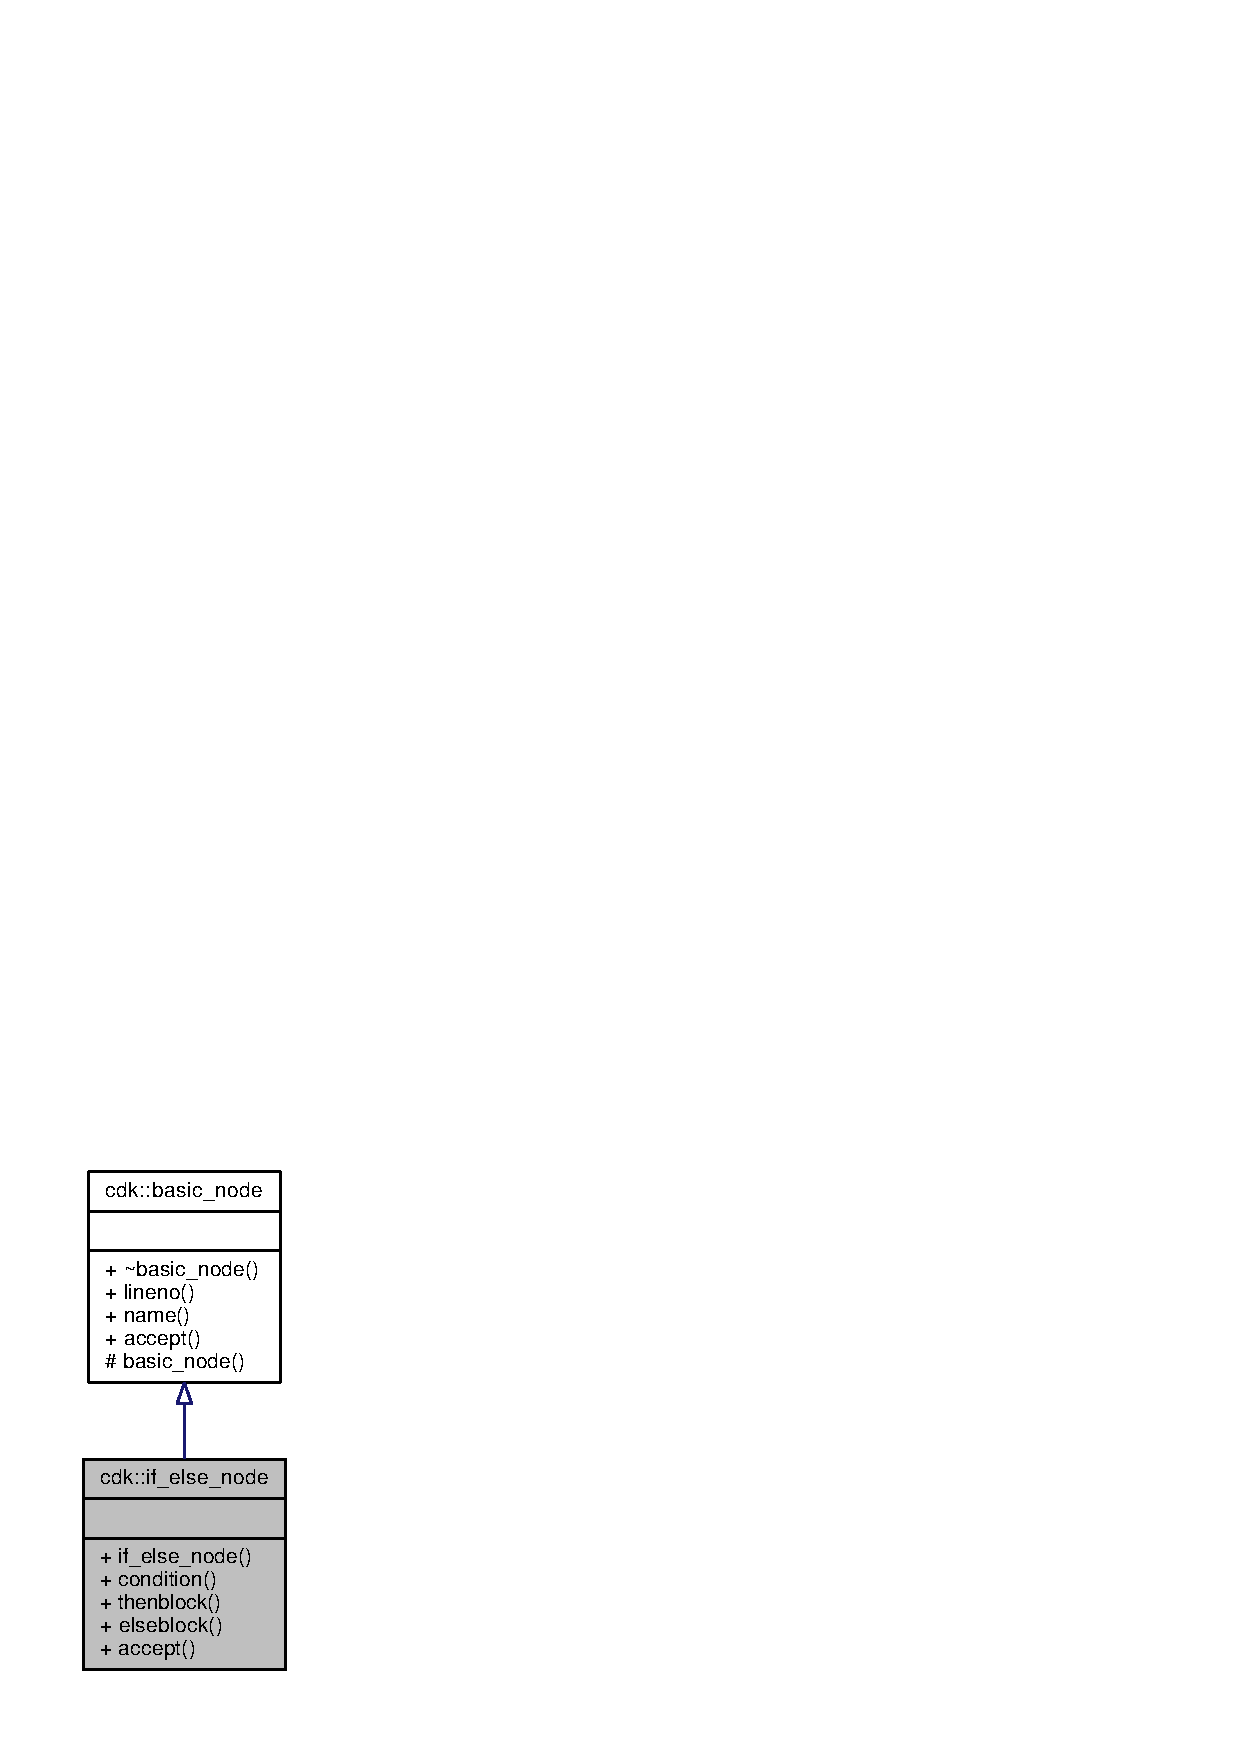
\includegraphics[width=141pt]{classcdk_1_1if__else__node__inherit__graph}
\end{center}
\end{figure}


Collaboration diagram for cdk\+:\+:if\+\_\+else\+\_\+node\+:
\nopagebreak
\begin{figure}[H]
\begin{center}
\leavevmode
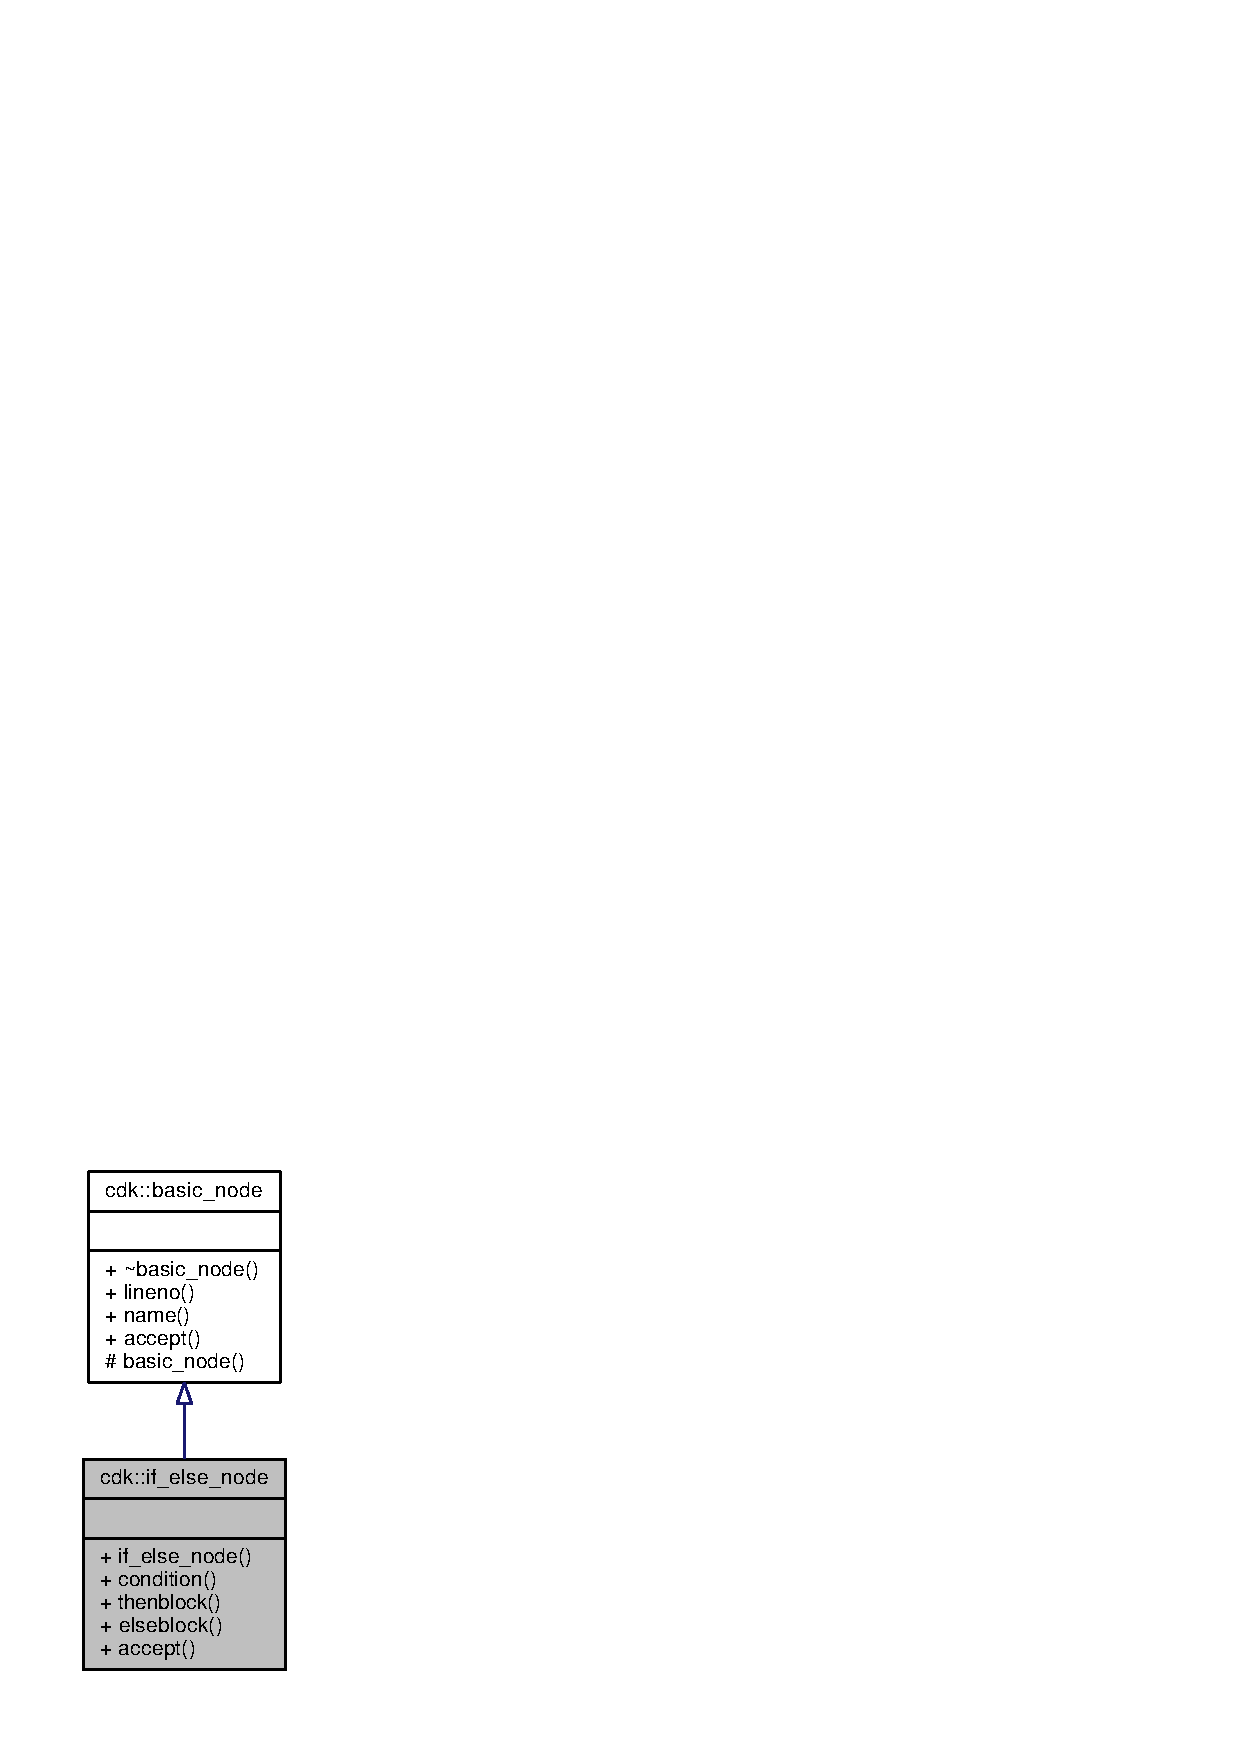
\includegraphics[width=141pt]{classcdk_1_1if__else__node__coll__graph}
\end{center}
\end{figure}
\subsection*{Public Member Functions}
\begin{DoxyCompactItemize}
\item 
{\bfseries if\+\_\+else\+\_\+node} (int {\bf lineno}, {\bf expression\+\_\+node} $\ast$condition, {\bf basic\+\_\+node} $\ast$thenblock, {\bf basic\+\_\+node} $\ast$elseblock)\label{classcdk_1_1if__else__node_a65d1fba860ae3c8bb5e793b76d7b2921}

\item 
{\bf expression\+\_\+node} $\ast$ {\bfseries condition} ()\label{classcdk_1_1if__else__node_a1d7ef51acf621b820e720488ca37bd5c}

\item 
{\bf basic\+\_\+node} $\ast$ {\bfseries thenblock} ()\label{classcdk_1_1if__else__node_a601df4f07b8a93995744f0262b69e63b}

\item 
{\bf basic\+\_\+node} $\ast$ {\bfseries elseblock} ()\label{classcdk_1_1if__else__node_a71bd0be67c2d9eaf83ed7896250e1e38}

\item 
void {\bf accept} ({\bf basic\+\_\+ast\+\_\+visitor} $\ast$sp, int level)
\end{DoxyCompactItemize}
\subsection*{Additional Inherited Members}


\subsection{Detailed Description}
Class for describing if-\/then-\/else nodes. 

Definition at line 12 of file if\+\_\+else\+\_\+node.\+h.



\subsection{Member Function Documentation}
\index{cdk\+::if\+\_\+else\+\_\+node@{cdk\+::if\+\_\+else\+\_\+node}!accept@{accept}}
\index{accept@{accept}!cdk\+::if\+\_\+else\+\_\+node@{cdk\+::if\+\_\+else\+\_\+node}}
\subsubsection[{accept}]{\setlength{\rightskip}{0pt plus 5cm}void cdk\+::if\+\_\+else\+\_\+node\+::accept (
\begin{DoxyParamCaption}
\item[{{\bf basic\+\_\+ast\+\_\+visitor} $\ast$}]{sp, }
\item[{int}]{level}
\end{DoxyParamCaption}
)\hspace{0.3cm}{\ttfamily [inline]}, {\ttfamily [virtual]}}\label{classcdk_1_1if__else__node_a348ea45d822a94125a12156c92db48a0}
Every node must provide this method.


\begin{DoxyParams}{Parameters}
{\em sp} & semantic processor visitor \\
\hline
{\em level} & syntactic tree level \\
\hline
\end{DoxyParams}


Implements {\bf cdk\+::basic\+\_\+node} \doxyref{}{p.}{classcdk_1_1basic__node_ab38adcbc95c46b809961278afae3bf05}.



Definition at line 32 of file if\+\_\+else\+\_\+node.\+h.



The documentation for this class was generated from the following file\+:\begin{DoxyCompactItemize}
\item 
ast/if\+\_\+else\+\_\+node.\+h\end{DoxyCompactItemize}

\section{cdk\+:\+:if\+\_\+node Class Reference}
\label{classcdk_1_1if__node}\index{cdk\+::if\+\_\+node@{cdk\+::if\+\_\+node}}


{\ttfamily \#include $<$if\+\_\+node.\+h$>$}



Inheritance diagram for cdk\+:\+:if\+\_\+node\+:
\nopagebreak
\begin{figure}[H]
\begin{center}
\leavevmode
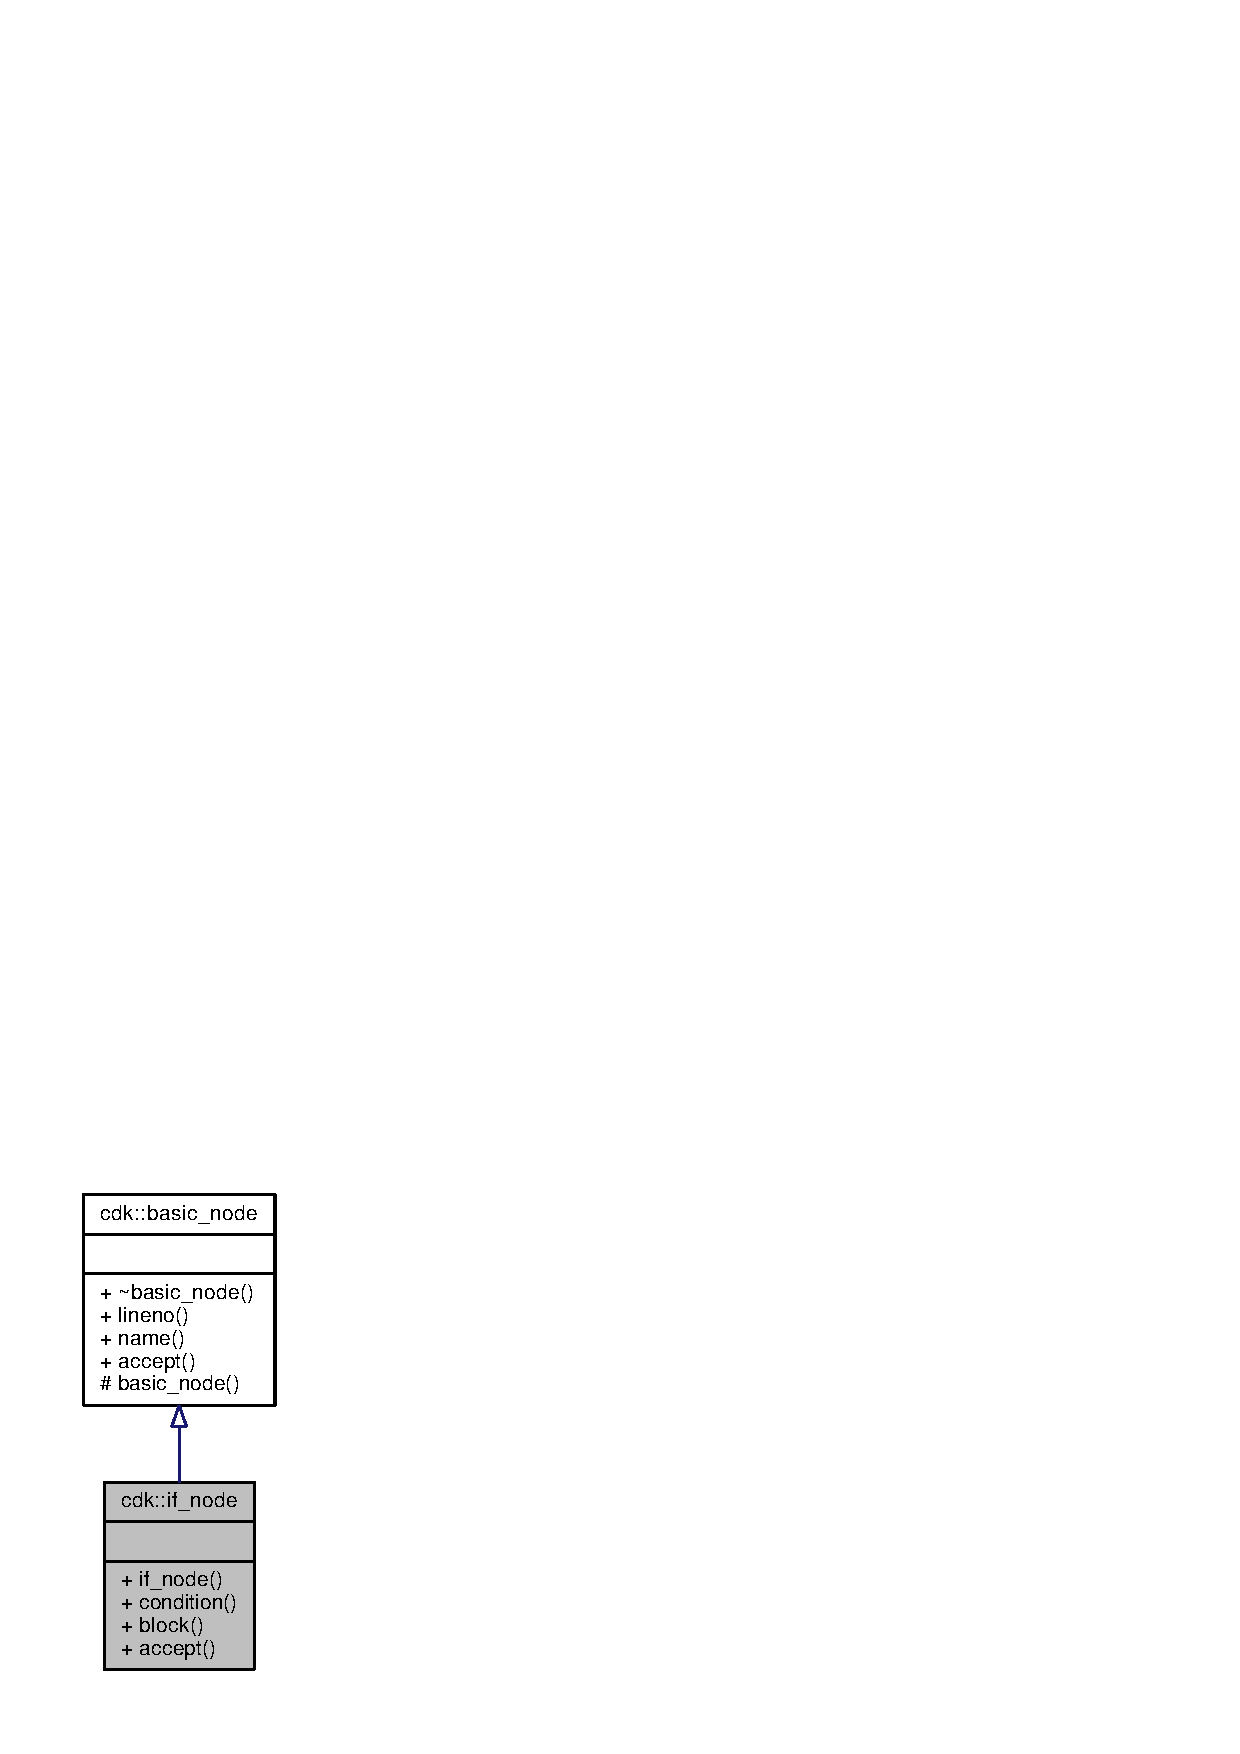
\includegraphics[width=136pt]{classcdk_1_1if__node__inherit__graph}
\end{center}
\end{figure}


Collaboration diagram for cdk\+:\+:if\+\_\+node\+:
\nopagebreak
\begin{figure}[H]
\begin{center}
\leavevmode
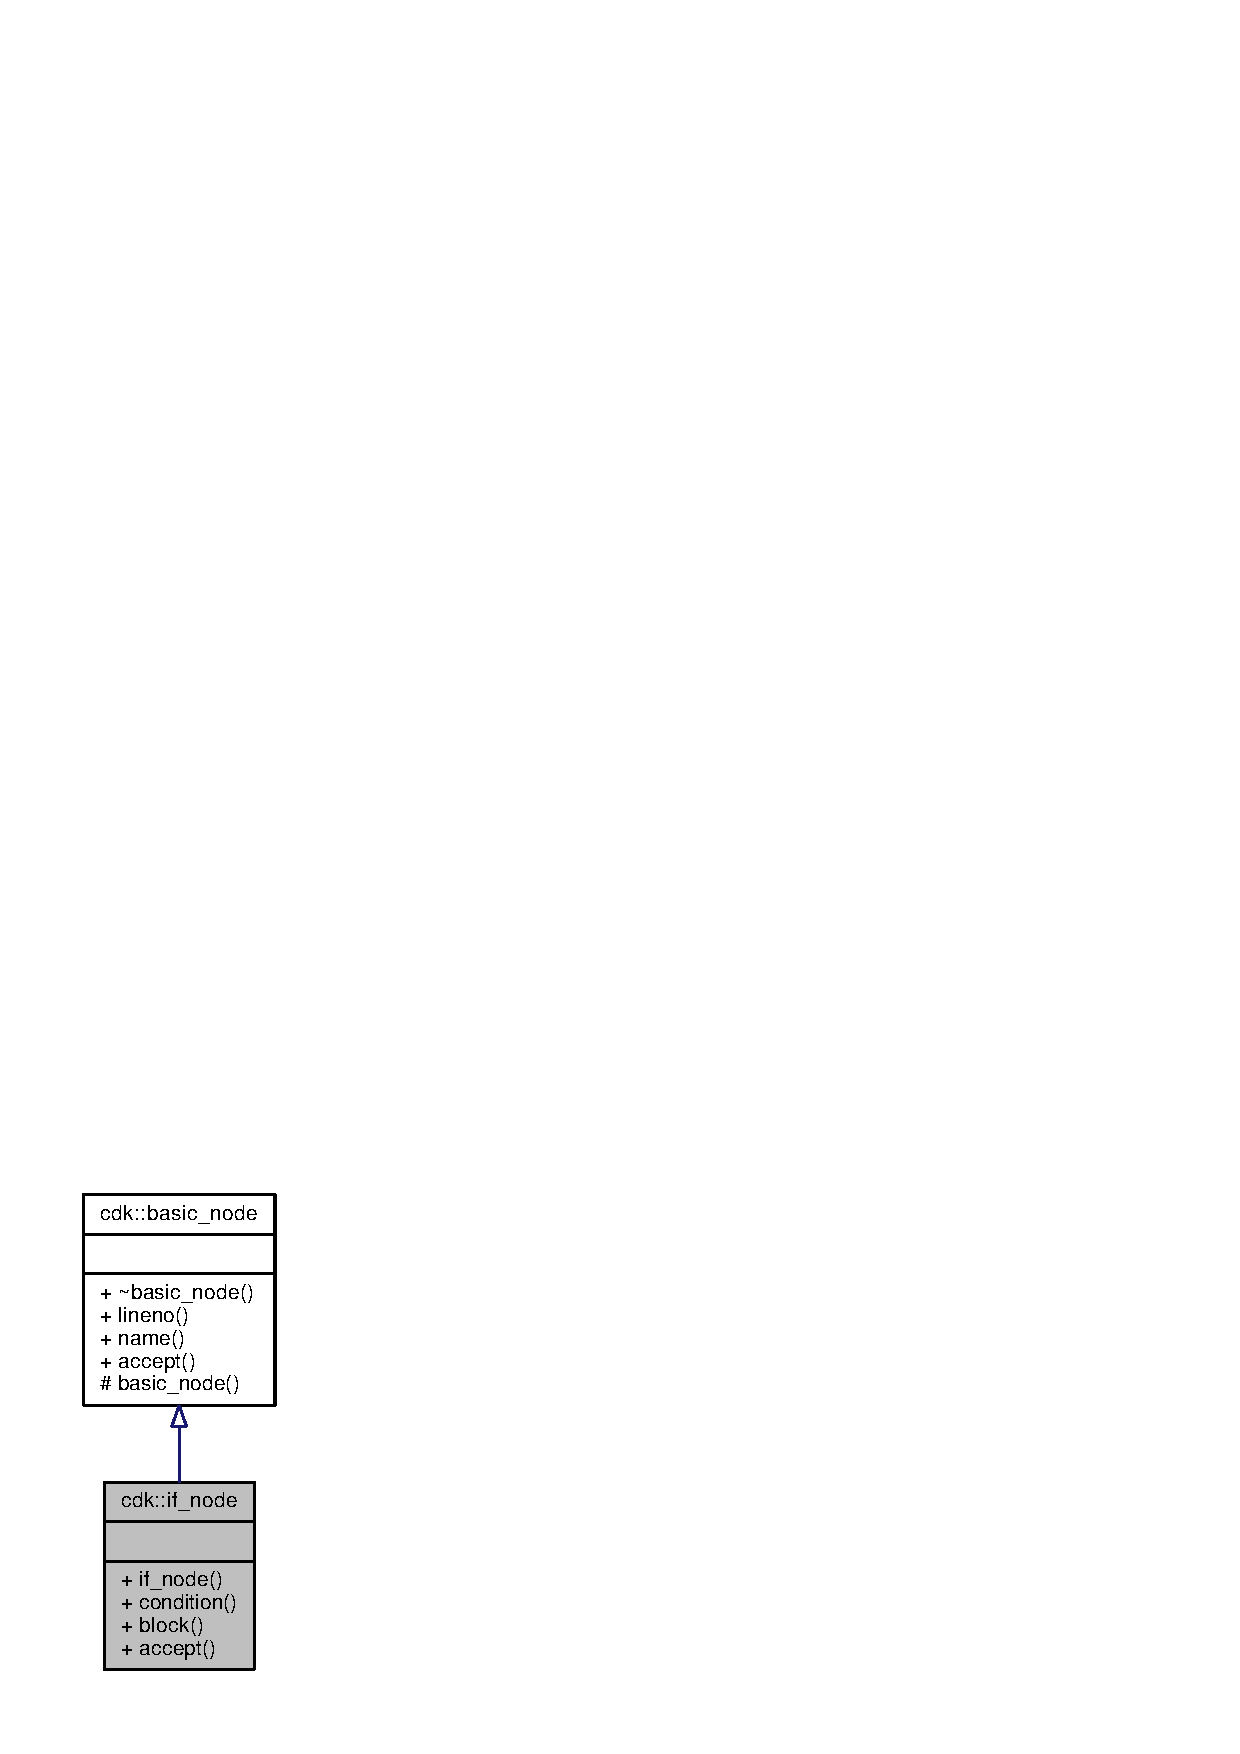
\includegraphics[width=136pt]{classcdk_1_1if__node__coll__graph}
\end{center}
\end{figure}
\subsection*{Public Member Functions}
\begin{DoxyCompactItemize}
\item 
{\bfseries if\+\_\+node} (int {\bf lineno}, {\bf expression\+\_\+node} $\ast$condition, {\bf basic\+\_\+node} $\ast$block)\label{classcdk_1_1if__node_a3a6b0c87cd8d0da3fea721d54552cf35}

\item 
{\bf expression\+\_\+node} $\ast$ {\bfseries condition} ()\label{classcdk_1_1if__node_a8f50b8064038b79a90a8e6f8fb6ba931}

\item 
{\bf basic\+\_\+node} $\ast$ {\bfseries block} ()\label{classcdk_1_1if__node_af9ac4278a9f42105d7f58555c5ebefe3}

\item 
void {\bf accept} ({\bf basic\+\_\+ast\+\_\+visitor} $\ast$sp, int level)
\end{DoxyCompactItemize}
\subsection*{Additional Inherited Members}


\subsection{Detailed Description}
Class for describing if-\/then nodes. 

Definition at line 12 of file if\+\_\+node.\+h.



\subsection{Member Function Documentation}
\index{cdk\+::if\+\_\+node@{cdk\+::if\+\_\+node}!accept@{accept}}
\index{accept@{accept}!cdk\+::if\+\_\+node@{cdk\+::if\+\_\+node}}
\subsubsection[{accept}]{\setlength{\rightskip}{0pt plus 5cm}void cdk\+::if\+\_\+node\+::accept (
\begin{DoxyParamCaption}
\item[{{\bf basic\+\_\+ast\+\_\+visitor} $\ast$}]{sp, }
\item[{int}]{level}
\end{DoxyParamCaption}
)\hspace{0.3cm}{\ttfamily [inline]}, {\ttfamily [virtual]}}\label{classcdk_1_1if__node_a3fee89ddd665238ed4db37fd73d01d81}
Every node must provide this method.


\begin{DoxyParams}{Parameters}
{\em sp} & semantic processor visitor \\
\hline
{\em level} & syntactic tree level \\
\hline
\end{DoxyParams}


Implements {\bf cdk\+::basic\+\_\+node} \doxyref{}{p.}{classcdk_1_1basic__node_ab38adcbc95c46b809961278afae3bf05}.



Definition at line 29 of file if\+\_\+node.\+h.



The documentation for this class was generated from the following file\+:\begin{DoxyCompactItemize}
\item 
ast/if\+\_\+node.\+h\end{DoxyCompactItemize}

\section{cdk\+:\+:integer\+\_\+node Class Reference}
\label{classcdk_1_1integer__node}\index{cdk\+::integer\+\_\+node@{cdk\+::integer\+\_\+node}}


{\ttfamily \#include $<$integer\+\_\+node.\+h$>$}



Inheritance diagram for cdk\+:\+:integer\+\_\+node\+:
\nopagebreak
\begin{figure}[H]
\begin{center}
\leavevmode
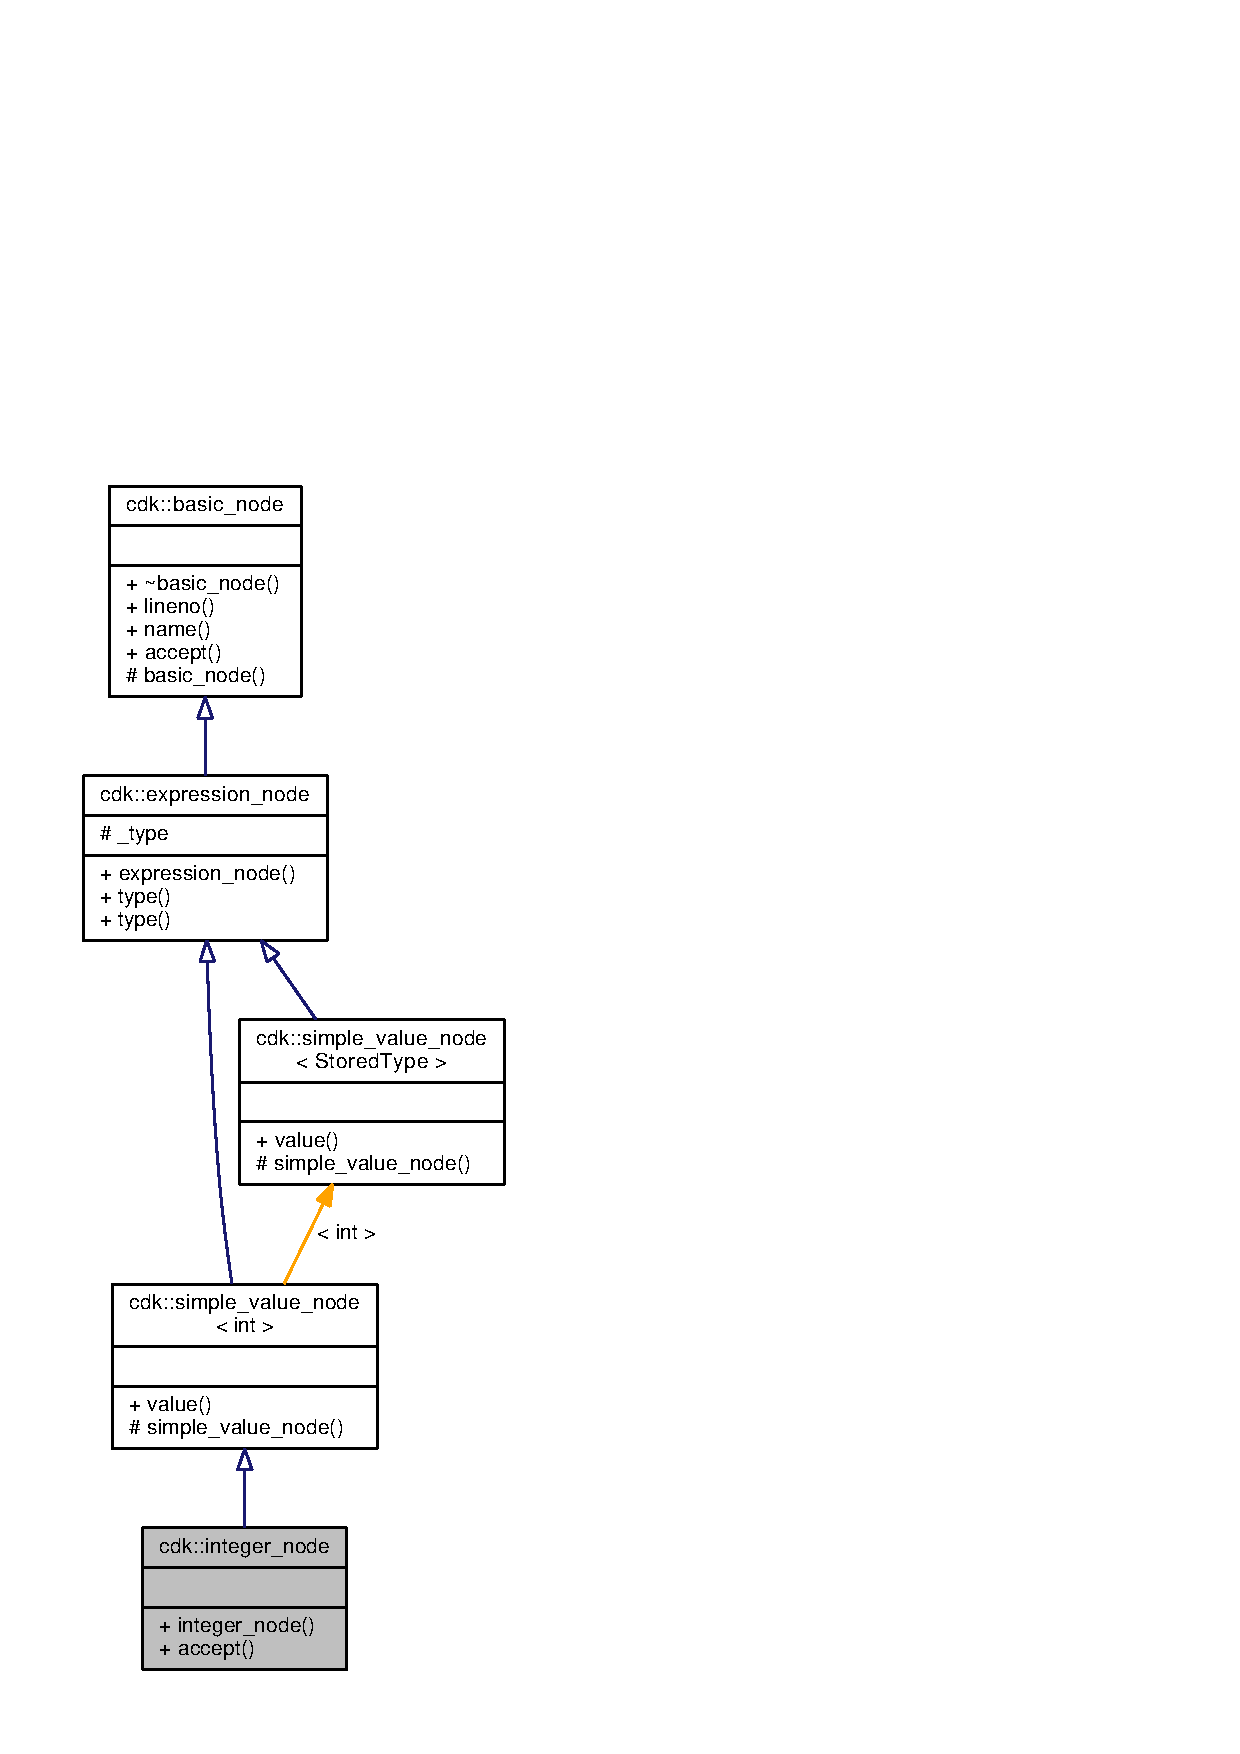
\includegraphics[height=550pt]{classcdk_1_1integer__node__inherit__graph}
\end{center}
\end{figure}


Collaboration diagram for cdk\+:\+:integer\+\_\+node\+:
\nopagebreak
\begin{figure}[H]
\begin{center}
\leavevmode
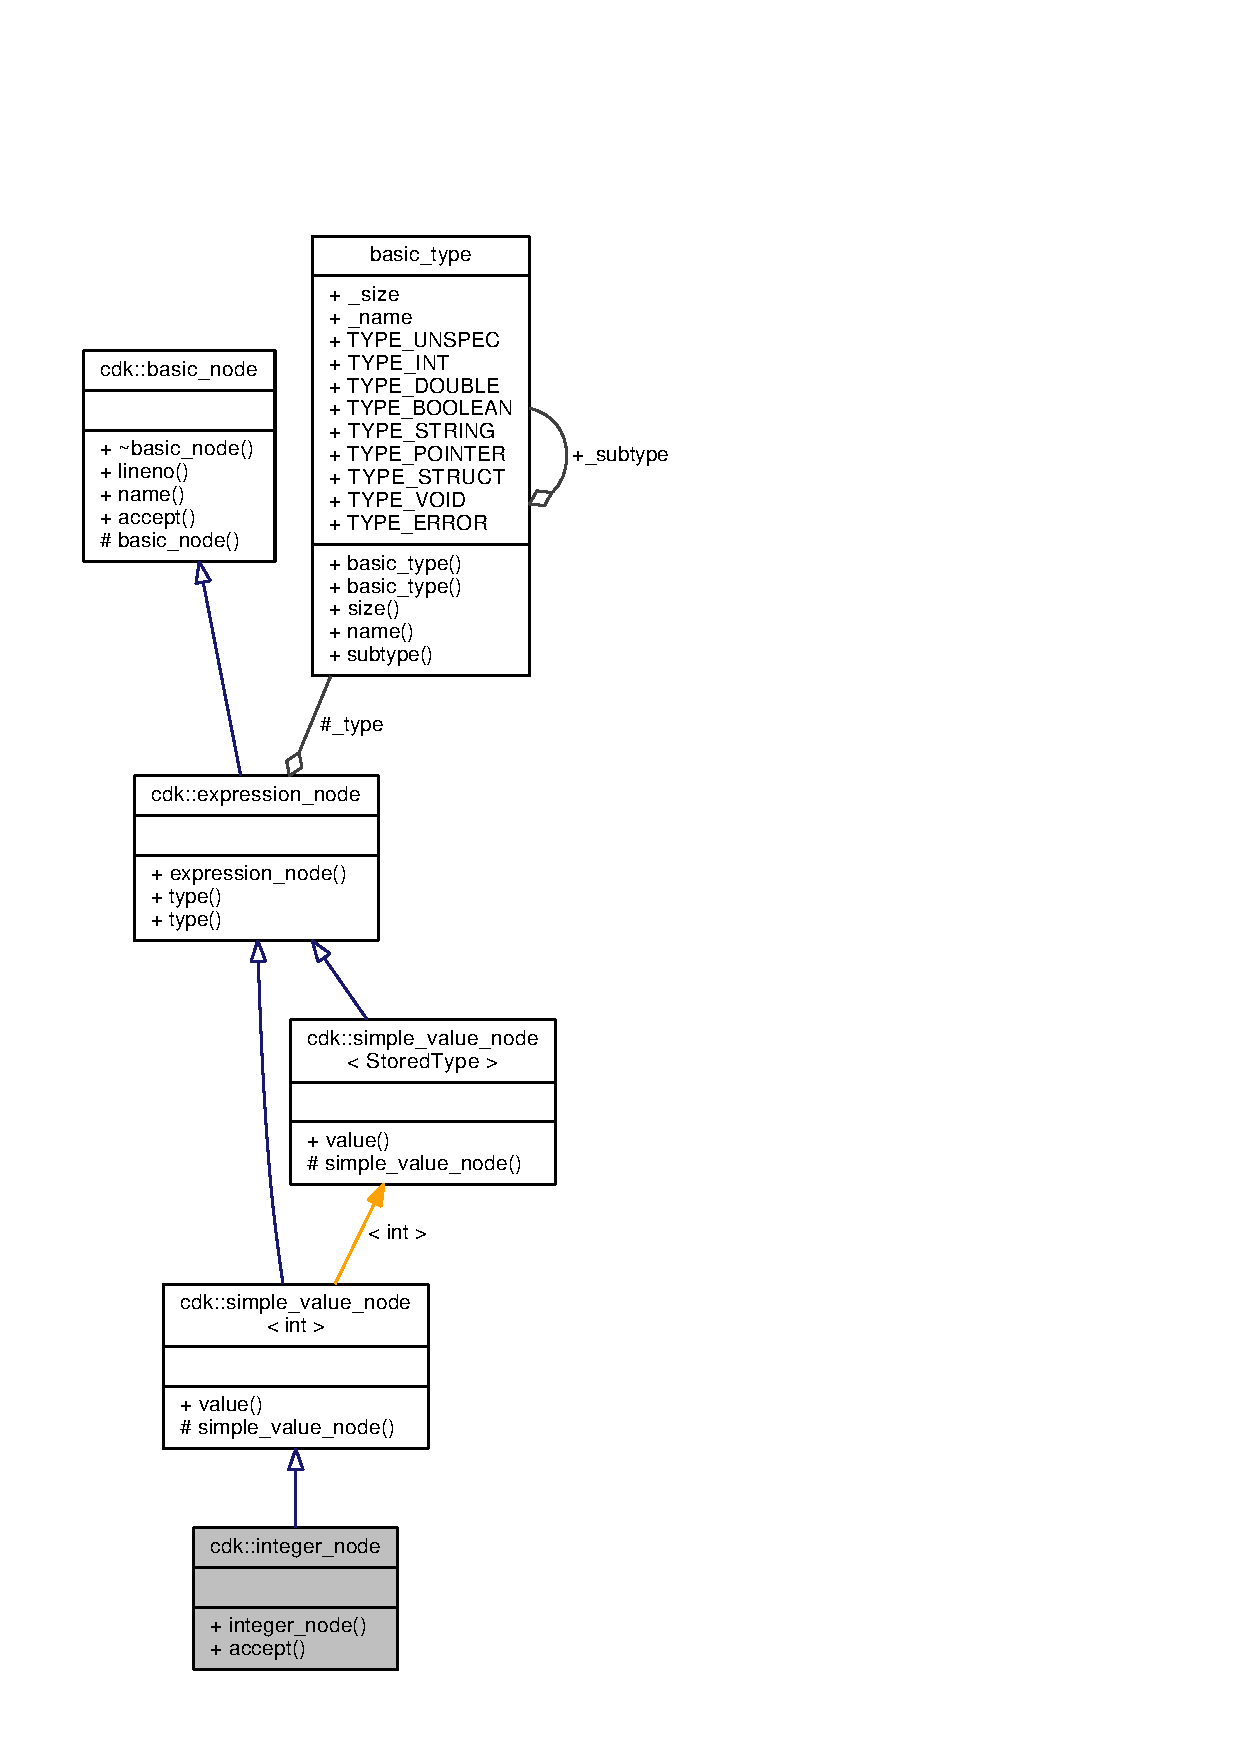
\includegraphics[height=550pt]{classcdk_1_1integer__node__coll__graph}
\end{center}
\end{figure}
\subsection*{Public Member Functions}
\begin{DoxyCompactItemize}
\item 
{\bfseries integer\+\_\+node} (int {\bf lineno}, int i)\label{classcdk_1_1integer__node_abb8794adaa28de8eb14f84e3cd3dbfde}

\item 
void {\bf accept} ({\bf basic\+\_\+ast\+\_\+visitor} $\ast$sp, int level)
\end{DoxyCompactItemize}
\subsection*{Additional Inherited Members}


\subsection{Detailed Description}
Class for describing syntactic tree leaves for holding integer values. 

Definition at line 12 of file integer\+\_\+node.\+h.



\subsection{Member Function Documentation}
\index{cdk\+::integer\+\_\+node@{cdk\+::integer\+\_\+node}!accept@{accept}}
\index{accept@{accept}!cdk\+::integer\+\_\+node@{cdk\+::integer\+\_\+node}}
\subsubsection[{accept}]{\setlength{\rightskip}{0pt plus 5cm}void cdk\+::integer\+\_\+node\+::accept (
\begin{DoxyParamCaption}
\item[{{\bf basic\+\_\+ast\+\_\+visitor} $\ast$}]{sp, }
\item[{int}]{level}
\end{DoxyParamCaption}
)\hspace{0.3cm}{\ttfamily [inline]}, {\ttfamily [virtual]}}\label{classcdk_1_1integer__node_a6b47d4c572b80bbaed62604a8c68788d}

\begin{DoxyParams}{Parameters}
{\em sp} & semantic processor visitor \\
\hline
{\em level} & syntactic tree level \\
\hline
\end{DoxyParams}


Implements {\bf cdk\+::basic\+\_\+node} \doxyref{}{p.}{classcdk_1_1basic__node_ab38adcbc95c46b809961278afae3bf05}.



Definition at line 22 of file integer\+\_\+node.\+h.



The documentation for this class was generated from the following file\+:\begin{DoxyCompactItemize}
\item 
ast/integer\+\_\+node.\+h\end{DoxyCompactItemize}

\section{cdk\+:\+:le\+\_\+node Class Reference}
\label{classcdk_1_1le__node}\index{cdk\+::le\+\_\+node@{cdk\+::le\+\_\+node}}


{\ttfamily \#include $<$le\+\_\+node.\+h$>$}



Inheritance diagram for cdk\+:\+:le\+\_\+node\+:
\nopagebreak
\begin{figure}[H]
\begin{center}
\leavevmode
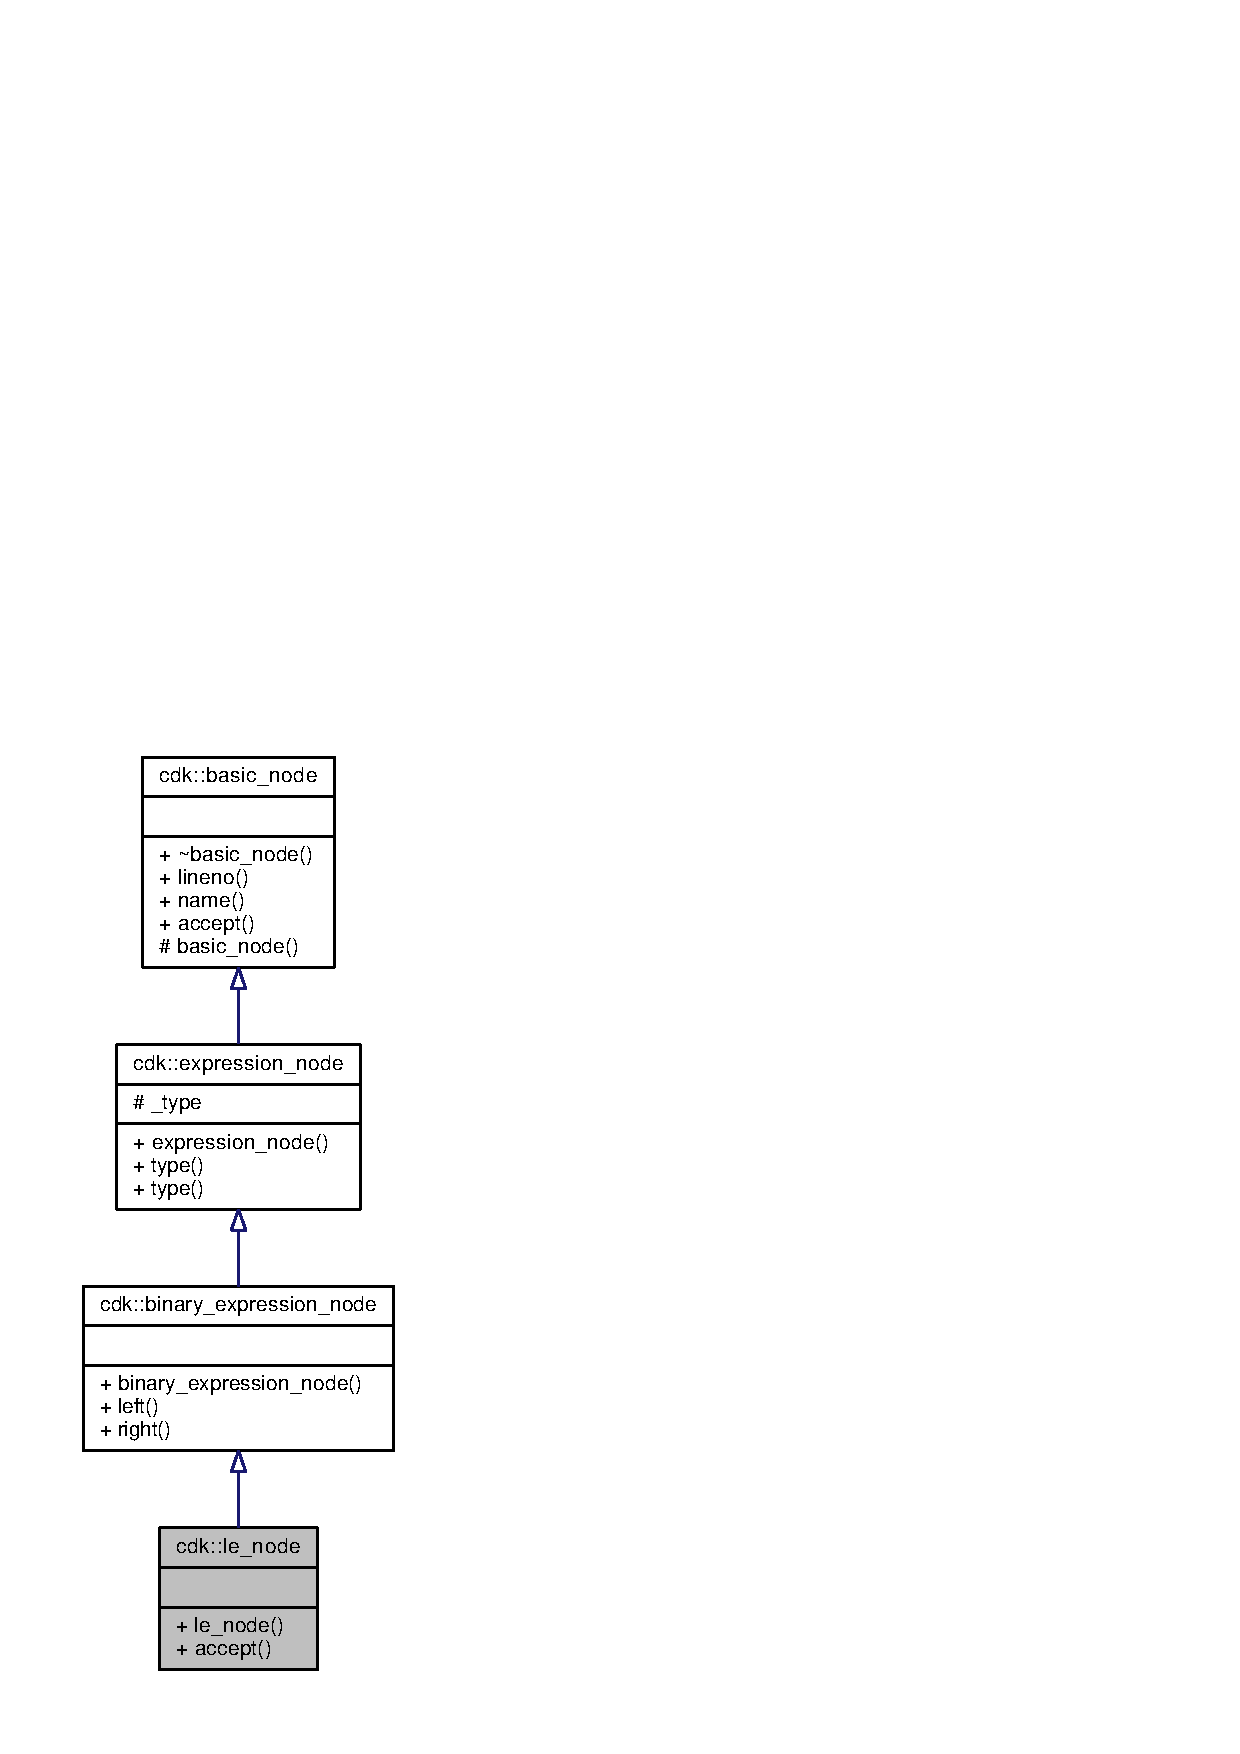
\includegraphics[width=193pt]{classcdk_1_1le__node__inherit__graph}
\end{center}
\end{figure}


Collaboration diagram for cdk\+:\+:le\+\_\+node\+:
\nopagebreak
\begin{figure}[H]
\begin{center}
\leavevmode
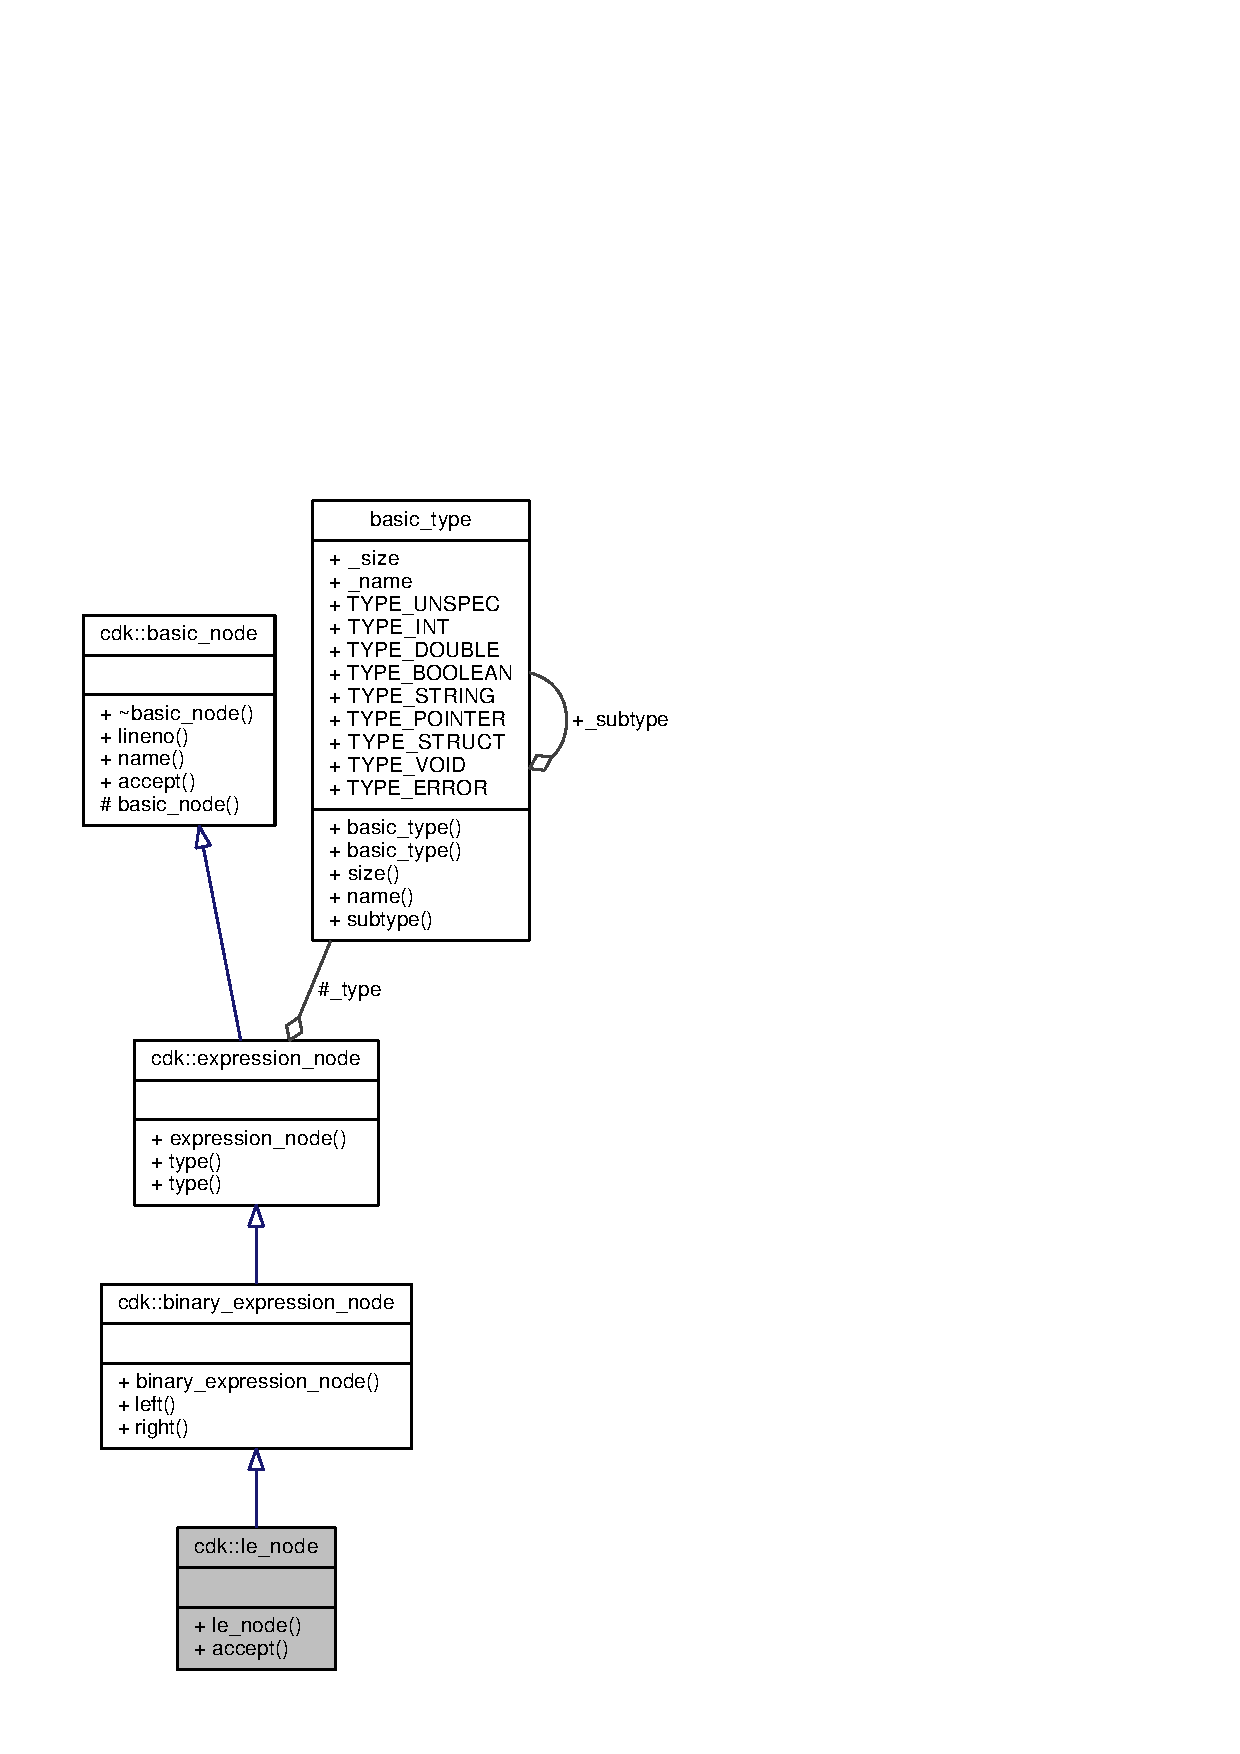
\includegraphics[height=550pt]{classcdk_1_1le__node__coll__graph}
\end{center}
\end{figure}
\subsection*{Public Member Functions}
\begin{DoxyCompactItemize}
\item 
{\bf le\+\_\+node} (int {\bf lineno}, {\bf expression\+\_\+node} $\ast$left, {\bf expression\+\_\+node} $\ast$right)
\item 
void {\bf accept} ({\bf basic\+\_\+ast\+\_\+visitor} $\ast$sp, int level)
\end{DoxyCompactItemize}
\subsection*{Additional Inherited Members}


\subsection{Detailed Description}
Class for describing the lower-\/than-\/or-\/equal operator 

Definition at line 12 of file le\+\_\+node.\+h.



\subsection{Constructor \& Destructor Documentation}
\index{cdk\+::le\+\_\+node@{cdk\+::le\+\_\+node}!le\+\_\+node@{le\+\_\+node}}
\index{le\+\_\+node@{le\+\_\+node}!cdk\+::le\+\_\+node@{cdk\+::le\+\_\+node}}
\subsubsection[{le\+\_\+node}]{\setlength{\rightskip}{0pt plus 5cm}cdk\+::le\+\_\+node\+::le\+\_\+node (
\begin{DoxyParamCaption}
\item[{int}]{lineno, }
\item[{{\bf expression\+\_\+node} $\ast$}]{left, }
\item[{{\bf expression\+\_\+node} $\ast$}]{right}
\end{DoxyParamCaption}
)\hspace{0.3cm}{\ttfamily [inline]}}\label{classcdk_1_1le__node_a2582bc8b99e25493ad4646156c3bed2d}

\begin{DoxyParams}{Parameters}
{\em lineno} & source code line number for this node \\
\hline
{\em left} & first operand \\
\hline
{\em right} & second operand \\
\hline
\end{DoxyParams}


Definition at line 19 of file le\+\_\+node.\+h.



\subsection{Member Function Documentation}
\index{cdk\+::le\+\_\+node@{cdk\+::le\+\_\+node}!accept@{accept}}
\index{accept@{accept}!cdk\+::le\+\_\+node@{cdk\+::le\+\_\+node}}
\subsubsection[{accept}]{\setlength{\rightskip}{0pt plus 5cm}void cdk\+::le\+\_\+node\+::accept (
\begin{DoxyParamCaption}
\item[{{\bf basic\+\_\+ast\+\_\+visitor} $\ast$}]{sp, }
\item[{int}]{level}
\end{DoxyParamCaption}
)\hspace{0.3cm}{\ttfamily [inline]}, {\ttfamily [virtual]}}\label{classcdk_1_1le__node_a4d3a01246f47dcb95ab7535a9047c9d6}

\begin{DoxyParams}{Parameters}
{\em sp} & semantic processor visitor \\
\hline
{\em level} & syntactic tree level \\
\hline
\end{DoxyParams}


Implements {\bf cdk\+::basic\+\_\+node} \doxyref{}{p.}{classcdk_1_1basic__node_ab38adcbc95c46b809961278afae3bf05}.



Definition at line 27 of file le\+\_\+node.\+h.



The documentation for this class was generated from the following file\+:\begin{DoxyCompactItemize}
\item 
ast/le\+\_\+node.\+h\end{DoxyCompactItemize}

\section{cdk\+:\+:lt\+\_\+node Class Reference}
\label{classcdk_1_1lt__node}\index{cdk\+::lt\+\_\+node@{cdk\+::lt\+\_\+node}}


{\ttfamily \#include $<$lt\+\_\+node.\+h$>$}



Inheritance diagram for cdk\+:\+:lt\+\_\+node\+:
\nopagebreak
\begin{figure}[H]
\begin{center}
\leavevmode
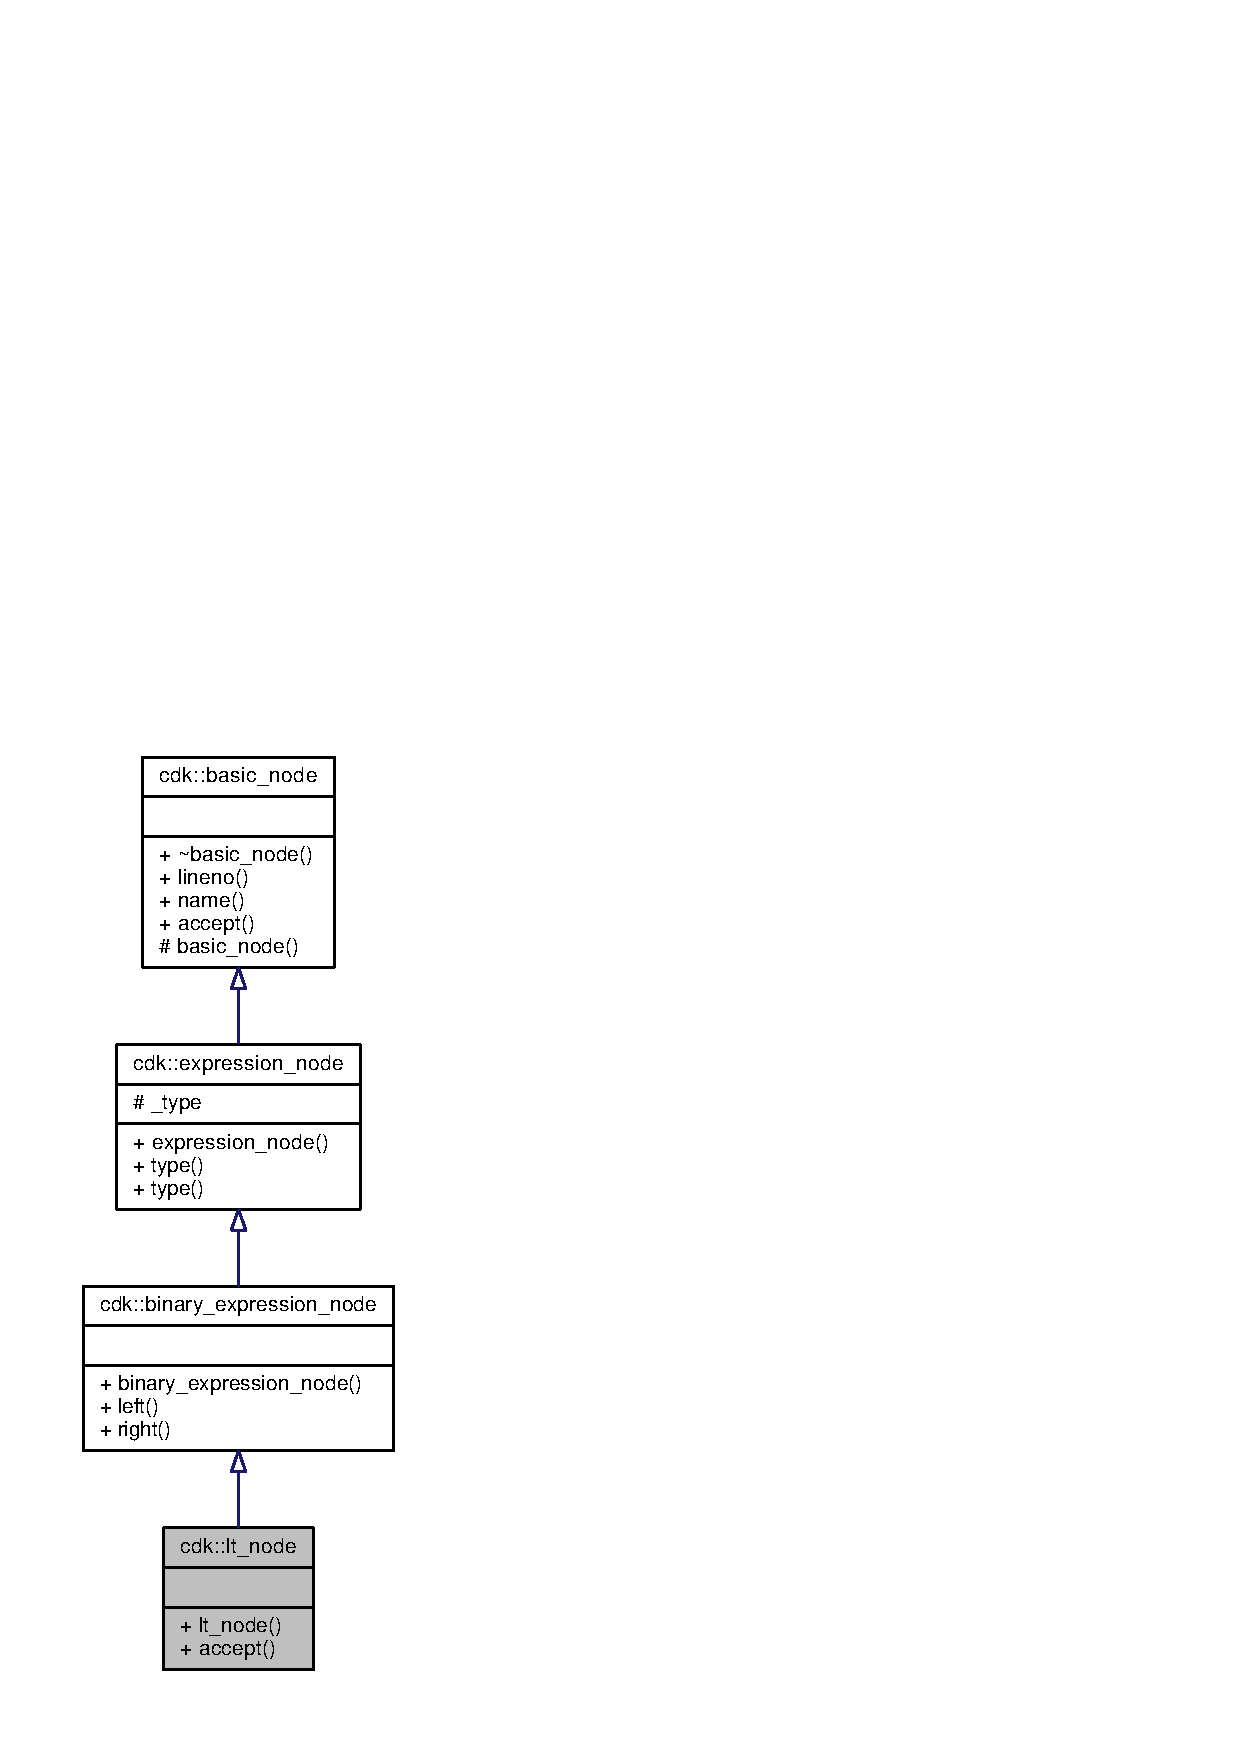
\includegraphics[width=193pt]{classcdk_1_1lt__node__inherit__graph}
\end{center}
\end{figure}


Collaboration diagram for cdk\+:\+:lt\+\_\+node\+:
\nopagebreak
\begin{figure}[H]
\begin{center}
\leavevmode
\includegraphics[height=550pt]{classcdk_1_1lt__node__coll__graph}
\end{center}
\end{figure}
\subsection*{Public Member Functions}
\begin{DoxyCompactItemize}
\item 
{\bf lt\+\_\+node} (int {\bf lineno}, {\bf expression\+\_\+node} $\ast$left, {\bf expression\+\_\+node} $\ast$right)
\item 
void {\bf accept} ({\bf basic\+\_\+ast\+\_\+visitor} $\ast$sp, int level)
\end{DoxyCompactItemize}
\subsection*{Additional Inherited Members}


\subsection{Detailed Description}
Class for describing the lower-\/than operator 

Definition at line 12 of file lt\+\_\+node.\+h.



\subsection{Constructor \& Destructor Documentation}
\index{cdk\+::lt\+\_\+node@{cdk\+::lt\+\_\+node}!lt\+\_\+node@{lt\+\_\+node}}
\index{lt\+\_\+node@{lt\+\_\+node}!cdk\+::lt\+\_\+node@{cdk\+::lt\+\_\+node}}
\subsubsection[{lt\+\_\+node}]{\setlength{\rightskip}{0pt plus 5cm}cdk\+::lt\+\_\+node\+::lt\+\_\+node (
\begin{DoxyParamCaption}
\item[{int}]{lineno, }
\item[{{\bf expression\+\_\+node} $\ast$}]{left, }
\item[{{\bf expression\+\_\+node} $\ast$}]{right}
\end{DoxyParamCaption}
)\hspace{0.3cm}{\ttfamily [inline]}}\label{classcdk_1_1lt__node_a2c3e8e72fb6385cc25ea2bc3cd594bc5}

\begin{DoxyParams}{Parameters}
{\em lineno} & source code line number for this node \\
\hline
{\em left} & first operand \\
\hline
{\em right} & second operand \\
\hline
\end{DoxyParams}


Definition at line 19 of file lt\+\_\+node.\+h.



\subsection{Member Function Documentation}
\index{cdk\+::lt\+\_\+node@{cdk\+::lt\+\_\+node}!accept@{accept}}
\index{accept@{accept}!cdk\+::lt\+\_\+node@{cdk\+::lt\+\_\+node}}
\subsubsection[{accept}]{\setlength{\rightskip}{0pt plus 5cm}void cdk\+::lt\+\_\+node\+::accept (
\begin{DoxyParamCaption}
\item[{{\bf basic\+\_\+ast\+\_\+visitor} $\ast$}]{sp, }
\item[{int}]{level}
\end{DoxyParamCaption}
)\hspace{0.3cm}{\ttfamily [inline]}, {\ttfamily [virtual]}}\label{classcdk_1_1lt__node_a6af8ca3130c12e7a38860c9e92aaaa97}

\begin{DoxyParams}{Parameters}
{\em sp} & semantic processor visitor \\
\hline
{\em level} & syntactic tree level \\
\hline
\end{DoxyParams}


Implements {\bf cdk\+::basic\+\_\+node} \doxyref{}{p.}{classcdk_1_1basic__node_ab38adcbc95c46b809961278afae3bf05}.



Definition at line 27 of file lt\+\_\+node.\+h.



The documentation for this class was generated from the following file\+:\begin{DoxyCompactItemize}
\item 
ast/lt\+\_\+node.\+h\end{DoxyCompactItemize}

\section{cdk\+:\+:mod\+\_\+node Class Reference}
\label{classcdk_1_1mod__node}\index{cdk\+::mod\+\_\+node@{cdk\+::mod\+\_\+node}}


{\ttfamily \#include $<$mod\+\_\+node.\+h$>$}



Inheritance diagram for cdk\+:\+:mod\+\_\+node\+:
\nopagebreak
\begin{figure}[H]
\begin{center}
\leavevmode
\includegraphics[width=193pt]{classcdk_1_1mod__node__inherit__graph}
\end{center}
\end{figure}


Collaboration diagram for cdk\+:\+:mod\+\_\+node\+:
\nopagebreak
\begin{figure}[H]
\begin{center}
\leavevmode
\includegraphics[height=550pt]{classcdk_1_1mod__node__coll__graph}
\end{center}
\end{figure}
\subsection*{Public Member Functions}
\begin{DoxyCompactItemize}
\item 
{\bf mod\+\_\+node} (int {\bf lineno}, {\bf expression\+\_\+node} $\ast$left, {\bf expression\+\_\+node} $\ast$right)
\item 
void {\bf accept} ({\bf basic\+\_\+ast\+\_\+visitor} $\ast$sp, int level)
\end{DoxyCompactItemize}
\subsection*{Additional Inherited Members}


\subsection{Detailed Description}
Class for describing the modulus operator 

Definition at line 12 of file mod\+\_\+node.\+h.



\subsection{Constructor \& Destructor Documentation}
\index{cdk\+::mod\+\_\+node@{cdk\+::mod\+\_\+node}!mod\+\_\+node@{mod\+\_\+node}}
\index{mod\+\_\+node@{mod\+\_\+node}!cdk\+::mod\+\_\+node@{cdk\+::mod\+\_\+node}}
\subsubsection[{mod\+\_\+node}]{\setlength{\rightskip}{0pt plus 5cm}cdk\+::mod\+\_\+node\+::mod\+\_\+node (
\begin{DoxyParamCaption}
\item[{int}]{lineno, }
\item[{{\bf expression\+\_\+node} $\ast$}]{left, }
\item[{{\bf expression\+\_\+node} $\ast$}]{right}
\end{DoxyParamCaption}
)\hspace{0.3cm}{\ttfamily [inline]}}\label{classcdk_1_1mod__node_a1c91715c67e3c28da9cfaeee494d5ad2}

\begin{DoxyParams}{Parameters}
{\em lineno} & source code line number for this node \\
\hline
{\em left} & first operand \\
\hline
{\em right} & second operand \\
\hline
\end{DoxyParams}


Definition at line 19 of file mod\+\_\+node.\+h.



\subsection{Member Function Documentation}
\index{cdk\+::mod\+\_\+node@{cdk\+::mod\+\_\+node}!accept@{accept}}
\index{accept@{accept}!cdk\+::mod\+\_\+node@{cdk\+::mod\+\_\+node}}
\subsubsection[{accept}]{\setlength{\rightskip}{0pt plus 5cm}void cdk\+::mod\+\_\+node\+::accept (
\begin{DoxyParamCaption}
\item[{{\bf basic\+\_\+ast\+\_\+visitor} $\ast$}]{sp, }
\item[{int}]{level}
\end{DoxyParamCaption}
)\hspace{0.3cm}{\ttfamily [inline]}, {\ttfamily [virtual]}}\label{classcdk_1_1mod__node_a990120f568275fb78d9adf66ec46434a}

\begin{DoxyParams}{Parameters}
{\em sp} & semantic processor visitor \\
\hline
{\em level} & syntactic tree level \\
\hline
\end{DoxyParams}


Implements {\bf cdk\+::basic\+\_\+node} \doxyref{}{p.}{classcdk_1_1basic__node_ab38adcbc95c46b809961278afae3bf05}.



Definition at line 27 of file mod\+\_\+node.\+h.



The documentation for this class was generated from the following file\+:\begin{DoxyCompactItemize}
\item 
ast/mod\+\_\+node.\+h\end{DoxyCompactItemize}

\section{cdk\+:\+:mul\+\_\+node Class Reference}
\label{classcdk_1_1mul__node}\index{cdk\+::mul\+\_\+node@{cdk\+::mul\+\_\+node}}


{\ttfamily \#include $<$mul\+\_\+node.\+h$>$}



Inheritance diagram for cdk\+:\+:mul\+\_\+node\+:
\nopagebreak
\begin{figure}[H]
\begin{center}
\leavevmode
\includegraphics[width=193pt]{classcdk_1_1mul__node__inherit__graph}
\end{center}
\end{figure}


Collaboration diagram for cdk\+:\+:mul\+\_\+node\+:
\nopagebreak
\begin{figure}[H]
\begin{center}
\leavevmode
\includegraphics[height=550pt]{classcdk_1_1mul__node__coll__graph}
\end{center}
\end{figure}
\subsection*{Public Member Functions}
\begin{DoxyCompactItemize}
\item 
{\bf mul\+\_\+node} (int {\bf lineno}, {\bf expression\+\_\+node} $\ast$left, {\bf expression\+\_\+node} $\ast$right)
\item 
void {\bf accept} ({\bf basic\+\_\+ast\+\_\+visitor} $\ast$sp, int level)
\end{DoxyCompactItemize}
\subsection*{Additional Inherited Members}


\subsection{Detailed Description}
Class for describing the multiplication operator 

Definition at line 12 of file mul\+\_\+node.\+h.



\subsection{Constructor \& Destructor Documentation}
\index{cdk\+::mul\+\_\+node@{cdk\+::mul\+\_\+node}!mul\+\_\+node@{mul\+\_\+node}}
\index{mul\+\_\+node@{mul\+\_\+node}!cdk\+::mul\+\_\+node@{cdk\+::mul\+\_\+node}}
\subsubsection[{mul\+\_\+node}]{\setlength{\rightskip}{0pt plus 5cm}cdk\+::mul\+\_\+node\+::mul\+\_\+node (
\begin{DoxyParamCaption}
\item[{int}]{lineno, }
\item[{{\bf expression\+\_\+node} $\ast$}]{left, }
\item[{{\bf expression\+\_\+node} $\ast$}]{right}
\end{DoxyParamCaption}
)\hspace{0.3cm}{\ttfamily [inline]}}\label{classcdk_1_1mul__node_a60637c0f4c7c68d97c5b895aa3b1c047}

\begin{DoxyParams}{Parameters}
{\em lineno} & source code line number for this node \\
\hline
{\em left} & first operand \\
\hline
{\em right} & second operand \\
\hline
\end{DoxyParams}


Definition at line 19 of file mul\+\_\+node.\+h.



\subsection{Member Function Documentation}
\index{cdk\+::mul\+\_\+node@{cdk\+::mul\+\_\+node}!accept@{accept}}
\index{accept@{accept}!cdk\+::mul\+\_\+node@{cdk\+::mul\+\_\+node}}
\subsubsection[{accept}]{\setlength{\rightskip}{0pt plus 5cm}void cdk\+::mul\+\_\+node\+::accept (
\begin{DoxyParamCaption}
\item[{{\bf basic\+\_\+ast\+\_\+visitor} $\ast$}]{sp, }
\item[{int}]{level}
\end{DoxyParamCaption}
)\hspace{0.3cm}{\ttfamily [inline]}, {\ttfamily [virtual]}}\label{classcdk_1_1mul__node_a82daadfc3194683a75c2e0630d09318d}

\begin{DoxyParams}{Parameters}
{\em sp} & semantic processor visitor \\
\hline
{\em level} & syntactic tree level \\
\hline
\end{DoxyParams}


Implements {\bf cdk\+::basic\+\_\+node} \doxyref{}{p.}{classcdk_1_1basic__node_ab38adcbc95c46b809961278afae3bf05}.



Definition at line 27 of file mul\+\_\+node.\+h.



The documentation for this class was generated from the following file\+:\begin{DoxyCompactItemize}
\item 
ast/mul\+\_\+node.\+h\end{DoxyCompactItemize}

\section{cdk\+:\+:ne\+\_\+node Class Reference}
\label{classcdk_1_1ne__node}\index{cdk\+::ne\+\_\+node@{cdk\+::ne\+\_\+node}}


{\ttfamily \#include $<$ne\+\_\+node.\+h$>$}



Inheritance diagram for cdk\+:\+:ne\+\_\+node\+:
\nopagebreak
\begin{figure}[H]
\begin{center}
\leavevmode
\includegraphics[width=193pt]{classcdk_1_1ne__node__inherit__graph}
\end{center}
\end{figure}


Collaboration diagram for cdk\+:\+:ne\+\_\+node\+:
\nopagebreak
\begin{figure}[H]
\begin{center}
\leavevmode
\includegraphics[height=550pt]{classcdk_1_1ne__node__coll__graph}
\end{center}
\end{figure}
\subsection*{Public Member Functions}
\begin{DoxyCompactItemize}
\item 
{\bf ne\+\_\+node} (int {\bf lineno}, {\bf expression\+\_\+node} $\ast$left, {\bf expression\+\_\+node} $\ast$right)
\item 
void {\bf accept} ({\bf basic\+\_\+ast\+\_\+visitor} $\ast$sp, int level)
\end{DoxyCompactItemize}
\subsection*{Additional Inherited Members}


\subsection{Detailed Description}
Class for describing the inequality operator 

Definition at line 12 of file ne\+\_\+node.\+h.



\subsection{Constructor \& Destructor Documentation}
\index{cdk\+::ne\+\_\+node@{cdk\+::ne\+\_\+node}!ne\+\_\+node@{ne\+\_\+node}}
\index{ne\+\_\+node@{ne\+\_\+node}!cdk\+::ne\+\_\+node@{cdk\+::ne\+\_\+node}}
\subsubsection[{ne\+\_\+node}]{\setlength{\rightskip}{0pt plus 5cm}cdk\+::ne\+\_\+node\+::ne\+\_\+node (
\begin{DoxyParamCaption}
\item[{int}]{lineno, }
\item[{{\bf expression\+\_\+node} $\ast$}]{left, }
\item[{{\bf expression\+\_\+node} $\ast$}]{right}
\end{DoxyParamCaption}
)\hspace{0.3cm}{\ttfamily [inline]}}\label{classcdk_1_1ne__node_ac7f41c158358fedaf2542936cc34e543}

\begin{DoxyParams}{Parameters}
{\em lineno} & source code line number for this node \\
\hline
{\em left} & first operand \\
\hline
{\em right} & second operand \\
\hline
\end{DoxyParams}


Definition at line 19 of file ne\+\_\+node.\+h.



\subsection{Member Function Documentation}
\index{cdk\+::ne\+\_\+node@{cdk\+::ne\+\_\+node}!accept@{accept}}
\index{accept@{accept}!cdk\+::ne\+\_\+node@{cdk\+::ne\+\_\+node}}
\subsubsection[{accept}]{\setlength{\rightskip}{0pt plus 5cm}void cdk\+::ne\+\_\+node\+::accept (
\begin{DoxyParamCaption}
\item[{{\bf basic\+\_\+ast\+\_\+visitor} $\ast$}]{sp, }
\item[{int}]{level}
\end{DoxyParamCaption}
)\hspace{0.3cm}{\ttfamily [inline]}, {\ttfamily [virtual]}}\label{classcdk_1_1ne__node_a66ac549e9cc152c1d4c23dfe0c3c3830}

\begin{DoxyParams}{Parameters}
{\em sp} & semantic processor visitor \\
\hline
{\em level} & syntactic tree level \\
\hline
\end{DoxyParams}


Implements {\bf cdk\+::basic\+\_\+node} \doxyref{}{p.}{classcdk_1_1basic__node_ab38adcbc95c46b809961278afae3bf05}.



Definition at line 27 of file ne\+\_\+node.\+h.



The documentation for this class was generated from the following file\+:\begin{DoxyCompactItemize}
\item 
ast/ne\+\_\+node.\+h\end{DoxyCompactItemize}

\section{cdk\+:\+:neg\+\_\+node Class Reference}
\label{classcdk_1_1neg__node}\index{cdk\+::neg\+\_\+node@{cdk\+::neg\+\_\+node}}


{\ttfamily \#include $<$neg\+\_\+node.\+h$>$}



Inheritance diagram for cdk\+:\+:neg\+\_\+node\+:
\nopagebreak
\begin{figure}[H]
\begin{center}
\leavevmode
\includegraphics[width=191pt]{classcdk_1_1neg__node__inherit__graph}
\end{center}
\end{figure}


Collaboration diagram for cdk\+:\+:neg\+\_\+node\+:
\nopagebreak
\begin{figure}[H]
\begin{center}
\leavevmode
\includegraphics[height=550pt]{classcdk_1_1neg__node__coll__graph}
\end{center}
\end{figure}
\subsection*{Public Member Functions}
\begin{DoxyCompactItemize}
\item 
{\bfseries neg\+\_\+node} (int {\bf lineno}, {\bf expression\+\_\+node} $\ast$arg)\label{classcdk_1_1neg__node_a08a049e7ffb26ab54087f63f67a9f66d}

\item 
void {\bf accept} ({\bf basic\+\_\+ast\+\_\+visitor} $\ast$sp, int level)
\end{DoxyCompactItemize}
\subsection*{Additional Inherited Members}


\subsection{Detailed Description}
Class for describing the negation operator 

Definition at line 12 of file neg\+\_\+node.\+h.



\subsection{Member Function Documentation}
\index{cdk\+::neg\+\_\+node@{cdk\+::neg\+\_\+node}!accept@{accept}}
\index{accept@{accept}!cdk\+::neg\+\_\+node@{cdk\+::neg\+\_\+node}}
\subsubsection[{accept}]{\setlength{\rightskip}{0pt plus 5cm}void cdk\+::neg\+\_\+node\+::accept (
\begin{DoxyParamCaption}
\item[{{\bf basic\+\_\+ast\+\_\+visitor} $\ast$}]{sp, }
\item[{int}]{level}
\end{DoxyParamCaption}
)\hspace{0.3cm}{\ttfamily [inline]}, {\ttfamily [virtual]}}\label{classcdk_1_1neg__node_ac49b8a32b9edaccfe38000cdb23d44c2}

\begin{DoxyParams}{Parameters}
{\em sp} & semantic processor visitor \\
\hline
{\em level} & syntactic tree level \\
\hline
\end{DoxyParams}


Implements {\bf cdk\+::basic\+\_\+node} \doxyref{}{p.}{classcdk_1_1basic__node_ab38adcbc95c46b809961278afae3bf05}.



Definition at line 22 of file neg\+\_\+node.\+h.



The documentation for this class was generated from the following file\+:\begin{DoxyCompactItemize}
\item 
ast/neg\+\_\+node.\+h\end{DoxyCompactItemize}

\section{cdk\+:\+:nil\+\_\+node Class Reference}
\label{classcdk_1_1nil__node}\index{cdk\+::nil\+\_\+node@{cdk\+::nil\+\_\+node}}


{\ttfamily \#include $<$nil\+\_\+node.\+h$>$}



Inheritance diagram for cdk\+:\+:nil\+\_\+node\+:
\nopagebreak
\begin{figure}[H]
\begin{center}
\leavevmode
\includegraphics[width=136pt]{classcdk_1_1nil__node__inherit__graph}
\end{center}
\end{figure}


Collaboration diagram for cdk\+:\+:nil\+\_\+node\+:
\nopagebreak
\begin{figure}[H]
\begin{center}
\leavevmode
\includegraphics[width=136pt]{classcdk_1_1nil__node__coll__graph}
\end{center}
\end{figure}
\subsection*{Public Member Functions}
\begin{DoxyCompactItemize}
\item 
{\bf nil\+\_\+node} (int {\bf lineno})
\item 
void {\bf accept} ({\bf basic\+\_\+ast\+\_\+visitor} $\ast$sp, int level)
\end{DoxyCompactItemize}
\subsection*{Additional Inherited Members}


\subsection{Detailed Description}
Class for describing empty nodes (leaves). The only data recorded by this type of node is the node's attribute (i.\+e., the mnemonic) and the source code line number. 

Definition at line 15 of file nil\+\_\+node.\+h.



\subsection{Constructor \& Destructor Documentation}
\index{cdk\+::nil\+\_\+node@{cdk\+::nil\+\_\+node}!nil\+\_\+node@{nil\+\_\+node}}
\index{nil\+\_\+node@{nil\+\_\+node}!cdk\+::nil\+\_\+node@{cdk\+::nil\+\_\+node}}
\subsubsection[{nil\+\_\+node}]{\setlength{\rightskip}{0pt plus 5cm}cdk\+::nil\+\_\+node\+::nil\+\_\+node (
\begin{DoxyParamCaption}
\item[{int}]{lineno}
\end{DoxyParamCaption}
)\hspace{0.3cm}{\ttfamily [inline]}}\label{classcdk_1_1nil__node_af83598e078cf7beb480658f7748f5529}
Simple constructor.


\begin{DoxyParams}{Parameters}
{\em lineno} & the source code line number corresponding to the node \\
\hline
\end{DoxyParams}


Definition at line 23 of file nil\+\_\+node.\+h.



\subsection{Member Function Documentation}
\index{cdk\+::nil\+\_\+node@{cdk\+::nil\+\_\+node}!accept@{accept}}
\index{accept@{accept}!cdk\+::nil\+\_\+node@{cdk\+::nil\+\_\+node}}
\subsubsection[{accept}]{\setlength{\rightskip}{0pt plus 5cm}void cdk\+::nil\+\_\+node\+::accept (
\begin{DoxyParamCaption}
\item[{{\bf basic\+\_\+ast\+\_\+visitor} $\ast$}]{sp, }
\item[{int}]{level}
\end{DoxyParamCaption}
)\hspace{0.3cm}{\ttfamily [inline]}, {\ttfamily [virtual]}}\label{classcdk_1_1nil__node_a98fe1eb1acb00d40f91a75a18db2e86d}

\begin{DoxyParams}{Parameters}
{\em sp} & semantic processor visitor \\
\hline
{\em level} & syntactic tree level \\
\hline
\end{DoxyParams}


Implements {\bf cdk\+::basic\+\_\+node} \doxyref{}{p.}{classcdk_1_1basic__node_ab38adcbc95c46b809961278afae3bf05}.



Definition at line 31 of file nil\+\_\+node.\+h.



The documentation for this class was generated from the following file\+:\begin{DoxyCompactItemize}
\item 
ast/nil\+\_\+node.\+h\end{DoxyCompactItemize}

\section{cdk\+:\+:null\+\_\+deleter Struct Reference}
\label{structcdk_1_1null__deleter}\index{cdk\+::null\+\_\+deleter@{cdk\+::null\+\_\+deleter}}


Collaboration diagram for cdk\+:\+:null\+\_\+deleter\+:
\nopagebreak
\begin{figure}[H]
\begin{center}
\leavevmode
\includegraphics[width=135pt]{structcdk_1_1null__deleter__coll__graph}
\end{center}
\end{figure}
\subsection*{Public Member Functions}
\begin{DoxyCompactItemize}
\item 
void {\bfseries operator()} (void $\ast$const)\label{structcdk_1_1null__deleter_ac230eb90b96a0413d7ca6c99b86c5fa2}

\end{DoxyCompactItemize}


\subsection{Detailed Description}


Definition at line 10 of file null\+\_\+deleter.\+h.



The documentation for this struct was generated from the following file\+:\begin{DoxyCompactItemize}
\item 
null\+\_\+deleter.\+h\end{DoxyCompactItemize}

\section{cdk\+:\+:postfix\+\_\+debug\+\_\+emitter Class Reference}
\label{classcdk_1_1postfix__debug__emitter}\index{cdk\+::postfix\+\_\+debug\+\_\+emitter@{cdk\+::postfix\+\_\+debug\+\_\+emitter}}


{\ttfamily \#include $<$postfix\+\_\+debug\+\_\+emitter.\+h$>$}



Inheritance diagram for cdk\+:\+:postfix\+\_\+debug\+\_\+emitter\+:
\nopagebreak
\begin{figure}[H]
\begin{center}
\leavevmode
\includegraphics[width=175pt]{classcdk_1_1postfix__debug__emitter__inherit__graph}
\end{center}
\end{figure}


Collaboration diagram for cdk\+:\+:postfix\+\_\+debug\+\_\+emitter\+:
\nopagebreak
\begin{figure}[H]
\begin{center}
\leavevmode
\includegraphics[width=175pt]{classcdk_1_1postfix__debug__emitter__coll__graph}
\end{center}
\end{figure}
\subsection*{Public Member Functions}
\begin{DoxyCompactItemize}
\item 
{\bfseries postfix\+\_\+debug\+\_\+emitter} (std\+::shared\+\_\+ptr$<$ {\bf compiler} $>$ \&{\bf compiler})\label{classcdk_1_1postfix__debug__emitter_ac144735dc1f967bd20d744ffc0006173}

\item 
void {\bfseries N\+O\+P} ()\label{classcdk_1_1postfix__debug__emitter_a3e2d86d30acf20ad5e8f1be90a464267}

\item 
void {\bfseries I\+N\+T} (int value)\label{classcdk_1_1postfix__debug__emitter_aab41a379957410b22b9915d7bcec405c}

\item 
void {\bfseries A\+D\+D} ()\label{classcdk_1_1postfix__debug__emitter_acad44057642996220d6991b955d0093f}

\item 
void {\bfseries S\+U\+B} ()\label{classcdk_1_1postfix__debug__emitter_a33d06ea7f5cc549ac9e6ae1b167d9366}

\item 
void {\bfseries M\+U\+L} ()\label{classcdk_1_1postfix__debug__emitter_ab9cbfa670707bea5cc5c98b0f7f9e9ea}

\item 
void {\bfseries D\+I\+V} ()\label{classcdk_1_1postfix__debug__emitter_a9166f30498740a0cf68173403875d728}

\item 
void {\bfseries M\+O\+D} ()\label{classcdk_1_1postfix__debug__emitter_a907a9c934dbe3744ad35b15557a0fc24}

\item 
void {\bfseries N\+E\+G} ()\label{classcdk_1_1postfix__debug__emitter_a603424a28230bf855c5680c16ac9c7ca}

\item 
void {\bfseries I\+N\+C\+R} (int value)\label{classcdk_1_1postfix__debug__emitter_a61f2e8993c1ac409114c5fdc433d8afc}

\item 
void {\bfseries D\+E\+C\+R} (int value)\label{classcdk_1_1postfix__debug__emitter_a45561c2c7f047ba6ae56579c280a1f65}

\item 
void {\bfseries G\+T} ()\label{classcdk_1_1postfix__debug__emitter_a6f01655f64ec4ca8ae610336154456df}

\item 
void {\bfseries G\+E} ()\label{classcdk_1_1postfix__debug__emitter_ac34e43628aa82b73251e14330ffe721c}

\item 
void {\bfseries L\+T} ()\label{classcdk_1_1postfix__debug__emitter_a48b0c29bc5fd178e8b23c590932a2b80}

\item 
void {\bfseries L\+E} ()\label{classcdk_1_1postfix__debug__emitter_a5883aa92c57dbdf1e4e39047fbf769db}

\item 
void {\bfseries E\+Q} ()\label{classcdk_1_1postfix__debug__emitter_a7d15c8c4ce6a6ced7748235f757d14ac}

\item 
void {\bfseries N\+E} ()\label{classcdk_1_1postfix__debug__emitter_a6033aded8929a944139ec7e70ee2b32f}

\item 
void {\bfseries A\+N\+D} ()\label{classcdk_1_1postfix__debug__emitter_a4a07204f2a05d81b4de3bc9935cf2904}

\item 
void {\bfseries O\+R} ()\label{classcdk_1_1postfix__debug__emitter_ad5e485369a95936f0d61ac7c2f24885f}

\item 
void {\bfseries X\+O\+R} ()\label{classcdk_1_1postfix__debug__emitter_a67c741da04d3e8c25783057f12fd5599}

\item 
void {\bfseries N\+O\+T} ()\label{classcdk_1_1postfix__debug__emitter_a1057eaae46a7aab6520d16032d129f81}

\item 
void {\bfseries R\+O\+T\+L} ()\label{classcdk_1_1postfix__debug__emitter_a3c74910b999ca2cad18052d8ab680837}

\item 
void {\bfseries R\+O\+T\+R} ()\label{classcdk_1_1postfix__debug__emitter_a4542c82531104b8cc9b3173f9051ca95}

\item 
void {\bfseries S\+H\+T\+L} ()\label{classcdk_1_1postfix__debug__emitter_a92a68458c967de963bb8c342ac67ba3b}

\item 
void {\bfseries S\+H\+T\+R\+U} ()\label{classcdk_1_1postfix__debug__emitter_a3638869152e91dbdb4ab68b180fe3ef9}

\item 
void {\bfseries S\+H\+T\+R\+S} ()\label{classcdk_1_1postfix__debug__emitter_aa8cfb68e6777133c790e0520fffadaeb}

\item 
void {\bfseries L\+O\+C\+A\+L} (int offset)\label{classcdk_1_1postfix__debug__emitter_a8b610509b95584c10d5c25e55ba75ae6}

\item 
void {\bfseries A\+D\+D\+R} (std\+::string label)\label{classcdk_1_1postfix__debug__emitter_a2c518b2fe083bf65223c7fc91d26907f}

\item 
void {\bfseries L\+O\+C\+V} (int offset)\label{classcdk_1_1postfix__debug__emitter_a0c07dfe4d651eaf8f672d38342bcd341}

\item 
void {\bfseries A\+D\+D\+R\+V} (std\+::string label)\label{classcdk_1_1postfix__debug__emitter_aaec34ef3f0a391104b8f9af14daf5ca3}

\item 
void {\bfseries L\+O\+C\+A} (int offset)\label{classcdk_1_1postfix__debug__emitter_ad24a4b5f3e3b87b3ac88a05108449b0b}

\item 
void {\bfseries A\+D\+D\+R\+A} (std\+::string label)\label{classcdk_1_1postfix__debug__emitter_aee4882bb988c2d2a6d7e7ad7948aaf08}

\item 
void {\bfseries L\+O\+A\+D} ()\label{classcdk_1_1postfix__debug__emitter_a87bfb50e52a0a6ed47e40654d2c113a4}

\item 
void {\bfseries S\+T\+O\+R\+E} ()\label{classcdk_1_1postfix__debug__emitter_a8e05c912ff34e61c9e61a245cc16e59f}

\item 
void {\bfseries L\+D\+C\+H\+R} ()\label{classcdk_1_1postfix__debug__emitter_a506ab67b1b719eae355ea6224f201872}

\item 
void {\bfseries S\+T\+C\+H\+R} ()\label{classcdk_1_1postfix__debug__emitter_a5667149a9fbb967b7d1bc2eff02d9666}

\item 
void {\bfseries L\+D16} ()\label{classcdk_1_1postfix__debug__emitter_ac25b8369942931e7977ea4d65feabcb1}

\item 
void {\bfseries S\+T16} ()\label{classcdk_1_1postfix__debug__emitter_a80cee2f2e8c697ef4e388c34709731d7}

\item 
void {\bfseries E\+N\+T\+E\+R} (size\+\_\+t bytes)\label{classcdk_1_1postfix__debug__emitter_aa0505817dba170c445f7d3c02cd7761c}

\item 
void {\bfseries S\+T\+A\+R\+T} ()\label{classcdk_1_1postfix__debug__emitter_a8f8fdac9a23ed75ed2df84d45b6836d0}

\item 
void {\bfseries A\+L\+L\+O\+C} ()\label{classcdk_1_1postfix__debug__emitter_af7c79d2f91f8f076addee1448be7f3c0}

\item 
void {\bfseries L\+E\+A\+V\+E} ()\label{classcdk_1_1postfix__debug__emitter_acad51aef16c01ee7d661bc90d09764a1}

\item 
void {\bfseries T\+R\+A\+S\+H} (int bytes)\label{classcdk_1_1postfix__debug__emitter_aa001d57e41d7d2c1d6ccc49f1d8d1e5e}

\item 
void {\bfseries C\+A\+L\+L} (std\+::string label)\label{classcdk_1_1postfix__debug__emitter_af09a47feb77467af88827f3fc8235625}

\item 
void {\bfseries R\+E\+T} ()\label{classcdk_1_1postfix__debug__emitter_a1ce768b85cc4bbefd7d4933c93704bdb}

\item 
void {\bfseries R\+E\+T\+N} (int bytes)\label{classcdk_1_1postfix__debug__emitter_a31cd54b8fed6bba134d9fa10295883a4}

\item 
void {\bfseries B\+R\+A\+N\+C\+H} ()\label{classcdk_1_1postfix__debug__emitter_aa4f9705c5db8565e9a83ed0ee1b08111}

\item 
void {\bfseries L\+E\+A\+P} ()\label{classcdk_1_1postfix__debug__emitter_acfc3aac9990b4ea6922dff2f658ba190}

\item 
void {\bfseries J\+M\+P} (std\+::string label)\label{classcdk_1_1postfix__debug__emitter_a9afb5e038b173b61723bb8ec4d377e97}

\item 
void {\bfseries J\+Z} (std\+::string label)\label{classcdk_1_1postfix__debug__emitter_a972c12217f05ebaaa00a2c021deb7a67}

\item 
void {\bfseries J\+N\+Z} (std\+::string label)\label{classcdk_1_1postfix__debug__emitter_a096187b72529a08bc0bf89cf9e768443}

\item 
void {\bfseries D\+U\+P} ()\label{classcdk_1_1postfix__debug__emitter_a92c2bee56314cf3df7bd00dedee0c84b}

\item 
void {\bfseries D\+D\+U\+P} ()\label{classcdk_1_1postfix__debug__emitter_ae430e45e7d9a9d4c51fe6a5dd748d1da}

\item 
void {\bfseries S\+W\+A\+P} ()\label{classcdk_1_1postfix__debug__emitter_af269d2d51b70848f0692b0695a6b41d4}

\item 
void {\bfseries S\+P} ()\label{classcdk_1_1postfix__debug__emitter_a6097d5e307a1b38c78ca8b2f26331ef2}

\item 
void {\bfseries P\+U\+S\+H} ()\label{classcdk_1_1postfix__debug__emitter_aa7a62b6532215faeadd94537a614f3e3}

\item 
void {\bfseries P\+O\+P} ()\label{classcdk_1_1postfix__debug__emitter_a6755eb8b0a4d83e8c11a97d49a9be68c}

\item 
void {\bfseries I2\+D} ()\label{classcdk_1_1postfix__debug__emitter_ad5d2004706c5cbcacd65bd737040c150}

\item 
void {\bfseries F2\+D} ()\label{classcdk_1_1postfix__debug__emitter_a87c7b74b6656022abc832d97577da230}

\item 
void {\bfseries D2\+I} ()\label{classcdk_1_1postfix__debug__emitter_a857d2e54ae5f743c6ce85d6921af9f83}

\item 
void {\bfseries D2\+F} ()\label{classcdk_1_1postfix__debug__emitter_a6f72556c60dd8100ea5eb7497a8a7a54}

\item 
void {\bfseries D\+A\+D\+D} ()\label{classcdk_1_1postfix__debug__emitter_a273979aaa6eafddd89609bf684b791fa}

\item 
void {\bfseries D\+S\+U\+B} ()\label{classcdk_1_1postfix__debug__emitter_ac41d5ba49b202bbb4412bd57b5019102}

\item 
void {\bfseries D\+M\+U\+L} ()\label{classcdk_1_1postfix__debug__emitter_ae1e775dbef6aa1848ecce580a629a169}

\item 
void {\bfseries D\+D\+I\+V} ()\label{classcdk_1_1postfix__debug__emitter_a8306a6613addf517e6b3ad3c412bcf7c}

\item 
void {\bfseries D\+C\+M\+P} ()\label{classcdk_1_1postfix__debug__emitter_a5b1e0d4c015447886236a327eeea9428}

\item 
void {\bfseries D\+N\+E\+G} ()\label{classcdk_1_1postfix__debug__emitter_a2f2582118db3dc3f9d15de3180702162}

\item 
void {\bfseries D\+L\+O\+A\+D} ()\label{classcdk_1_1postfix__debug__emitter_a13020985435cc5600dfeee8084180f4f}

\item 
void {\bfseries D\+S\+T\+O\+R\+E} ()\label{classcdk_1_1postfix__debug__emitter_aa288d93a5edffc955aaaf4dd208dc67a}

\item 
void {\bfseries D\+P\+U\+S\+H} ()\label{classcdk_1_1postfix__debug__emitter_a1b88107d91c403e5ee1e383513e65775}

\item 
void {\bfseries D\+P\+O\+P} ()\label{classcdk_1_1postfix__debug__emitter_a3c6c230ecd69cf5d418f73aa478131fd}

\item 
void {\bfseries N\+I\+L} ()\label{classcdk_1_1postfix__debug__emitter_a6d39b6d8db806d5695d6559b4498a765}

\item 
void {\bfseries T\+E\+X\+T} ()\label{classcdk_1_1postfix__debug__emitter_a3c93f49ec6c06df44864a96efa19d1f0}

\item 
void {\bfseries R\+O\+D\+A\+T\+A} ()\label{classcdk_1_1postfix__debug__emitter_a5cd431f11fa3ab52823592f475e78570}

\item 
void {\bfseries D\+A\+T\+A} ()\label{classcdk_1_1postfix__debug__emitter_aa96a83413d0e44ed18656bf18212f2ee}

\item 
void {\bfseries B\+S\+S} ()\label{classcdk_1_1postfix__debug__emitter_ac1ecf31945f1afa75f88082b963b14d5}

\item 
void {\bfseries A\+L\+I\+G\+N} ()\label{classcdk_1_1postfix__debug__emitter_ae3a086cce1afc1ba3b8a82f3888e9448}

\item 
void {\bfseries E\+X\+T\+E\+R\+N} (std\+::string label)\label{classcdk_1_1postfix__debug__emitter_ad19790fc7c413f55d3503c30c12375f1}

\item 
void {\bfseries C\+O\+M\+M\+O\+N} (int value)\label{classcdk_1_1postfix__debug__emitter_a82b2aec820b210bd6ec018d81e61c368}

\item 
void {\bfseries G\+L\+O\+B\+A\+L} (const char $\ast$label, std\+::string type)\label{classcdk_1_1postfix__debug__emitter_a3f9f8b1fd4fbfd78daa80728d11f9df1}

\item 
void {\bfseries G\+L\+O\+B\+A\+L} (std\+::string label, std\+::string type)\label{classcdk_1_1postfix__debug__emitter_a77403bf1f70e78b766c32a9b6e73cacc}

\item 
void {\bfseries L\+A\+B\+E\+L} (std\+::string label)\label{classcdk_1_1postfix__debug__emitter_ac005b818e2054e0d339ac4cbc148b064}

\item 
void {\bfseries C\+O\+N\+S\+T} (int value)\label{classcdk_1_1postfix__debug__emitter_a3be7c77942d9c7cb56cdf002d24f02c6}

\item 
void {\bfseries S\+T\+R} (std\+::string value)\label{classcdk_1_1postfix__debug__emitter_afe9fc20b8599f6b552c25d495a82da17}

\item 
void {\bfseries C\+H\+A\+R} (char value)\label{classcdk_1_1postfix__debug__emitter_a698c0180e1ecd9065cea7da81f5d4025}

\item 
void {\bfseries I\+D} (std\+::string label)\label{classcdk_1_1postfix__debug__emitter_a704cf2ee915fe5856d357ec2be35e9db}

\item 
void {\bfseries B\+Y\+T\+E} (int value)\label{classcdk_1_1postfix__debug__emitter_a2b75e17bbe158f5dbe6501f3fdecf3b5}

\item 
void {\bfseries F\+L\+O\+A\+T} (float value)\label{classcdk_1_1postfix__debug__emitter_ac1c06771b22cda667bb39a2d6304ac18}

\item 
void {\bfseries D\+O\+U\+B\+L\+E} (double value)\label{classcdk_1_1postfix__debug__emitter_aa5a7258ebbdd242d83c5a18511021581}

\item 
void {\bfseries U\+L\+D\+C\+H\+R} ()\label{classcdk_1_1postfix__debug__emitter_ac88d7c6b314c4b5e6832751d3d4faaba}

\item 
void {\bfseries U\+L\+D16} ()\label{classcdk_1_1postfix__debug__emitter_ac10c70509ceff4fa2e0d920f6de55a9a}

\item 
void {\bfseries U\+D\+I\+V} ()\label{classcdk_1_1postfix__debug__emitter_a4858c2c539de032e8dccc916bd3593e7}

\item 
void {\bfseries U\+M\+O\+D} ()\label{classcdk_1_1postfix__debug__emitter_a47fdc2e1fd410e89449a478b23b93cc1}

\item 
void {\bfseries U\+G\+T} ()\label{classcdk_1_1postfix__debug__emitter_abc8f2232c81ebae09924f227f2921de0}

\item 
void {\bfseries U\+G\+E} ()\label{classcdk_1_1postfix__debug__emitter_a738f7fd41b171b437070c32ab426e2d2}

\item 
void {\bfseries U\+L\+T} ()\label{classcdk_1_1postfix__debug__emitter_a86469610a1393ce449efb5a6b2dc89a0}

\item 
void {\bfseries U\+L\+E} ()\label{classcdk_1_1postfix__debug__emitter_abb016b0a0afe01737a6967d1498c073f}

\item 
void {\bfseries J\+E\+Q} (std\+::string label)\label{classcdk_1_1postfix__debug__emitter_a802f8efe07633ca4fb912ebe00d36de3}

\item 
void {\bfseries J\+N\+E} (std\+::string label)\label{classcdk_1_1postfix__debug__emitter_a87f047742cf68c950b3617ca0ec200d5}

\item 
void {\bfseries J\+G\+T} (std\+::string label)\label{classcdk_1_1postfix__debug__emitter_ae1216ab573747c1f50e7bbabd8b2b8f2}

\item 
void {\bfseries J\+G\+E} (std\+::string label)\label{classcdk_1_1postfix__debug__emitter_afbca64d657a622c1a80a5a47a1b66ed5}

\item 
void {\bfseries J\+L\+T} (std\+::string label)\label{classcdk_1_1postfix__debug__emitter_addfe997b95fbeca594e83a8b747cc9c6}

\item 
void {\bfseries J\+L\+E} (std\+::string label)\label{classcdk_1_1postfix__debug__emitter_a34aef2e9f9a6fa93d96a4a2c2aff5317}

\item 
void {\bfseries J\+U\+G\+T} (std\+::string label)\label{classcdk_1_1postfix__debug__emitter_a0eaf22e4cec8840b6d44c549681f4a12}

\item 
void {\bfseries J\+U\+G\+E} (std\+::string label)\label{classcdk_1_1postfix__debug__emitter_af7b2bbf8a7ca1694ea75158534ded20f}

\item 
void {\bfseries J\+U\+L\+T} (std\+::string label)\label{classcdk_1_1postfix__debug__emitter_a1dcc7605e58d588c27e5b8e57a88ca15}

\item 
void {\bfseries J\+U\+L\+E} (std\+::string label)\label{classcdk_1_1postfix__debug__emitter_af6246322b38e28dbba72983f9e008524}

\end{DoxyCompactItemize}
\subsection*{Additional Inherited Members}


\subsection{Detailed Description}
Class \doxyref{postfix\+\_\+debug\+\_\+emitter}{p.}{classcdk_1_1postfix__debug__emitter}\+: generate P\+F assembly (debug only). \begin{DoxySeeAlso}{See also}
\doxyref{basic\+\_\+postfix\+\_\+emitter}{p.}{classcdk_1_1basic__postfix__emitter} 
\end{DoxySeeAlso}


Definition at line 13 of file postfix\+\_\+debug\+\_\+emitter.\+h.



The documentation for this class was generated from the following file\+:\begin{DoxyCompactItemize}
\item 
emitters/postfix\+\_\+debug\+\_\+emitter.\+h\end{DoxyCompactItemize}

\section{cdk\+:\+:postfix\+\_\+ix86\+\_\+emitter Class Reference}
\label{classcdk_1_1postfix__ix86__emitter}\index{cdk\+::postfix\+\_\+ix86\+\_\+emitter@{cdk\+::postfix\+\_\+ix86\+\_\+emitter}}


{\ttfamily \#include $<$postfix\+\_\+ix86\+\_\+emitter.\+h$>$}



Inheritance diagram for cdk\+:\+:postfix\+\_\+ix86\+\_\+emitter\+:
\nopagebreak
\begin{figure}[H]
\begin{center}
\leavevmode
\includegraphics[width=175pt]{classcdk_1_1postfix__ix86__emitter__inherit__graph}
\end{center}
\end{figure}


Collaboration diagram for cdk\+:\+:postfix\+\_\+ix86\+\_\+emitter\+:
\nopagebreak
\begin{figure}[H]
\begin{center}
\leavevmode
\includegraphics[width=175pt]{classcdk_1_1postfix__ix86__emitter__coll__graph}
\end{center}
\end{figure}
\subsection*{Public Member Functions}
\begin{DoxyCompactItemize}
\item 
{\bfseries postfix\+\_\+ix86\+\_\+emitter} (std\+::shared\+\_\+ptr$<$ {\bf compiler} $>$ \&{\bf compiler})\label{classcdk_1_1postfix__ix86__emitter_aa7d7bf9c95b4b2e4f1a963baa06700f2}

\item 
void {\bfseries O\+R\+I\+G} (int pos)\label{classcdk_1_1postfix__ix86__emitter_a046a6b984956e48ed3071bfdcba14ac5}

\item 
void {\bfseries E\+Q\+U} (std\+::string label, int value)\label{classcdk_1_1postfix__ix86__emitter_a9822a6ba2da140ccbc77cc48c51c3409}

\item 
void {\bfseries W\+O\+R\+D} (std\+::string label, int value)\label{classcdk_1_1postfix__ix86__emitter_aee8c89e354c578bb69c7be509ed19aef}

\item 
void {\bfseries S\+T\+R} (std\+::string label, std\+::string value)\label{classcdk_1_1postfix__ix86__emitter_a0cbf82132ad51092eb516f279b7691f1}

\item 
void {\bfseries T\+A\+B} (std\+::string label, int value)\label{classcdk_1_1postfix__ix86__emitter_a6b906cf332180a194ce60a42a9093c59}

\item 
void {\bfseries A\+D\+D} ()\label{classcdk_1_1postfix__ix86__emitter_a07351ab388d89aa51819a4dcb9472afe}

\item 
void {\bfseries A\+D\+D\+C} ()\label{classcdk_1_1postfix__ix86__emitter_a1548906d6384a16814d5bc3c07ec7c4e}

\item 
void {\bfseries A\+N\+D} ()\label{classcdk_1_1postfix__ix86__emitter_ae57d4ba81a42454fb2522cba9f1a47dc}

\item 
void {\bfseries B\+R\+C\+O\+N\+D} (std\+::string cond, std\+::string value)\label{classcdk_1_1postfix__ix86__emitter_a4521aeb29218e86a013ec9d81fcaeb68}

\item 
void {\bfseries B\+R} (std\+::string label)\label{classcdk_1_1postfix__ix86__emitter_ae75e5da6525aca913dc6db8a6646ebbd}

\item 
void {\bfseries C\+A\+L\+L} (std\+::string value)\label{classcdk_1_1postfix__ix86__emitter_aaa7e0ec5934b34b8ae5ed439f437cf99}

\item 
void {\bfseries C\+A\+L\+L\+C\+O\+N\+D} (std\+::string cond, std\+::string value)\label{classcdk_1_1postfix__ix86__emitter_a068d7e0d8ad1f00affa3f5b9cc2e5a14}

\item 
void {\bfseries C\+L\+C} ()\label{classcdk_1_1postfix__ix86__emitter_a40419d9fc89d0d8d1c05859d939e6bf0}

\item 
void {\bfseries C\+M\+C} ()\label{classcdk_1_1postfix__ix86__emitter_a0b69d7464befa541de661049966ee68a}

\item 
void {\bfseries C\+M\+P} ()\label{classcdk_1_1postfix__ix86__emitter_a894beb37b1c8624b6cb8253deae581d9}

\item 
void {\bfseries C\+O\+M} ()\label{classcdk_1_1postfix__ix86__emitter_a3ef1c20dad5c507b3cc7c3de320405b5}

\item 
void {\bfseries D\+E\+C} ()\label{classcdk_1_1postfix__ix86__emitter_ad9b1451ee73063a0bea38d494e891259}

\item 
void {\bfseries D\+I\+V} ()\label{classcdk_1_1postfix__ix86__emitter_a26325e9e51eda2ee46afb8243012ca46}

\item 
void {\bfseries D\+S\+I} ()\label{classcdk_1_1postfix__ix86__emitter_ae3a1e0c69d145c86901795aa32c8461a}

\item 
void {\bfseries E\+N\+I} ()\label{classcdk_1_1postfix__ix86__emitter_a421530fa8eb9a7846c7fdfb7a072c25a}

\item 
void {\bfseries I\+N\+C} ()\label{classcdk_1_1postfix__ix86__emitter_a7f20c5c7ac162239491c17eabb6d0c50}

\item 
void {\bfseries I\+N\+T} (int value)\label{classcdk_1_1postfix__ix86__emitter_ad96ca972823798ee328b54879f37a305}

\item 
void {\bfseries J\+M\+P} (std\+::string value)\label{classcdk_1_1postfix__ix86__emitter_a8c0dd44eaffa149c6001ad30fe7bd997}

\item 
void {\bfseries J\+M\+P\+C\+O\+N\+D} (std\+::string cond, std\+::string value)\label{classcdk_1_1postfix__ix86__emitter_a395e075bbf612b6f54782acd9a3aa143}

\item 
void {\bfseries M\+O\+V} ()\label{classcdk_1_1postfix__ix86__emitter_a09c2e45b1bc6942dc62e128b25aa6b16}

\item 
void {\bfseries M\+U\+L} ()\label{classcdk_1_1postfix__ix86__emitter_a81a8b9634cff7bccdec7c047ff8e87dd}

\item 
void {\bfseries M\+V\+B\+H} ()\label{classcdk_1_1postfix__ix86__emitter_aa5a94bb163081a20c307bbc06a6b3639}

\item 
void {\bfseries M\+V\+B\+L} ()\label{classcdk_1_1postfix__ix86__emitter_a5b455ac012866ac9503510c7919f63cb}

\item 
void {\bfseries N\+E\+G} ()\label{classcdk_1_1postfix__ix86__emitter_a9b9ab201deb2975ebffbd1b4ed065fd6}

\item 
void {\bfseries N\+O\+P} ()\label{classcdk_1_1postfix__ix86__emitter_ae5ae25018f54e7d86ff8eec7e8e07ab1}

\item 
void {\bfseries O\+R} ()\label{classcdk_1_1postfix__ix86__emitter_a51f69ea808217820156f791f6f2dda2c}

\item 
void {\bfseries P\+O\+P} ()\label{classcdk_1_1postfix__ix86__emitter_aae72dae4135373ba7ae257a704912068}

\item 
void {\bfseries P\+U\+S\+H} (int value)\label{classcdk_1_1postfix__ix86__emitter_ad94868e98d4d9d17f627b5708f5efc1c}

\item 
void {\bfseries R\+E\+T} ()\label{classcdk_1_1postfix__ix86__emitter_a9598410e14e2e5e228087de94f0c089f}

\item 
void {\bfseries R\+E\+T\+N} (int value)\label{classcdk_1_1postfix__ix86__emitter_a7543cacc44dab659e2af52aed17fc466}

\item 
void {\bfseries R\+O\+L} (int value)\label{classcdk_1_1postfix__ix86__emitter_a6fec0fe2b77a638bfd2bac5615ae6692}

\item 
void {\bfseries R\+O\+L\+C} (int value)\label{classcdk_1_1postfix__ix86__emitter_a114b69cc38c31e285199effc2830a442}

\item 
void {\bfseries R\+O\+R} (int value)\label{classcdk_1_1postfix__ix86__emitter_a7cb314439d29095043cb2dfdf834f5fc}

\item 
void {\bfseries R\+O\+R\+C} (int value)\label{classcdk_1_1postfix__ix86__emitter_ad19672467e41ddc54f0d462dc612f1ef}

\item 
void {\bfseries R\+T\+I} ()\label{classcdk_1_1postfix__ix86__emitter_aa653911e44c26b24734e55baf74e2b1a}

\item 
void {\bfseries S\+H\+L} (int value)\label{classcdk_1_1postfix__ix86__emitter_a7dcfd116cc994d75df8d854c8bf30626}

\item 
void {\bfseries S\+H\+L\+A} (int value)\label{classcdk_1_1postfix__ix86__emitter_af763b5a579af6cea068f66873f68e1fa}

\item 
void {\bfseries S\+H\+R} (int value)\label{classcdk_1_1postfix__ix86__emitter_ab4a8e8d14b5cd921fa1ddb147187a3b2}

\item 
void {\bfseries S\+H\+R\+A} (int value)\label{classcdk_1_1postfix__ix86__emitter_aa06aab08d636711b7c9b859c2e5c0e59}

\item 
void {\bfseries S\+T\+C} ()\label{classcdk_1_1postfix__ix86__emitter_a644dc25a9380242f858fef15e348c477}

\item 
void {\bfseries S\+U\+B} ()\label{classcdk_1_1postfix__ix86__emitter_a5211ce64f64abdf55e80461ae1c00c10}

\item 
void {\bfseries S\+U\+B\+B} ()\label{classcdk_1_1postfix__ix86__emitter_aa055d7d9905e2692f2e046cdc7580715}

\item 
void {\bfseries T\+E\+S\+T} ()\label{classcdk_1_1postfix__ix86__emitter_acc30425a8a791462ba68c56ce36f918e}

\item 
void {\bfseries X\+C\+H} ()\label{classcdk_1_1postfix__ix86__emitter_a9530b2bf9e03a75c8a8ff55ce9e8b106}

\item 
void {\bfseries X\+O\+R} ()\label{classcdk_1_1postfix__ix86__emitter_a331861f7d167d6d153528a3ed5fb8a68}

\item 
void {\bfseries L\+A\+B\+E\+L} (std\+::string label)\label{classcdk_1_1postfix__ix86__emitter_a3f4f32b93246b93aa7ee284b367ff03b}

\end{DoxyCompactItemize}
\subsection*{Additional Inherited Members}


\subsection{Detailed Description}
Class \doxyref{postfix\+\_\+ix86\+\_\+emitter}{p.}{classcdk_1_1postfix__ix86__emitter}\+: emitter for yasm/nasm code. 

Definition at line 14 of file postfix\+\_\+ix86\+\_\+emitter.\+h.



The documentation for this class was generated from the following file\+:\begin{DoxyCompactItemize}
\item 
emitters/postfix\+\_\+ix86\+\_\+emitter.\+h\end{DoxyCompactItemize}

\section{cdk\+:\+:sequence\+\_\+node Class Reference}
\label{classcdk_1_1sequence__node}\index{cdk\+::sequence\+\_\+node@{cdk\+::sequence\+\_\+node}}


{\ttfamily \#include $<$sequence\+\_\+node.\+h$>$}



Inheritance diagram for cdk\+:\+:sequence\+\_\+node\+:
\nopagebreak
\begin{figure}[H]
\begin{center}
\leavevmode
\includegraphics[width=157pt]{classcdk_1_1sequence__node__inherit__graph}
\end{center}
\end{figure}


Collaboration diagram for cdk\+:\+:sequence\+\_\+node\+:
\nopagebreak
\begin{figure}[H]
\begin{center}
\leavevmode
\includegraphics[width=157pt]{classcdk_1_1sequence__node__coll__graph}
\end{center}
\end{figure}
\subsection*{Public Member Functions}
\begin{DoxyCompactItemize}
\item 
{\bf sequence\+\_\+node} (int {\bf lineno}, {\bf basic\+\_\+node} $\ast$item, {\bf sequence\+\_\+node} $\ast$sequence=nullptr)
\item 
{\bf $\sim$sequence\+\_\+node} ()
\item 
{\bf basic\+\_\+node} $\ast$ {\bfseries node} (size\+\_\+t i)\label{classcdk_1_1sequence__node_a017eab5a8c90230655352b1551309719}

\item 
sequence\+\_\+type \& {\bfseries nodes} ()\label{classcdk_1_1sequence__node_ab98d492dfee088fb31299b93731027b4}

\item 
size\+\_\+t {\bfseries size} ()\label{classcdk_1_1sequence__node_ae59040d020ea3e42311595c267ca2486}

\item 
void {\bf accept} ({\bf basic\+\_\+ast\+\_\+visitor} $\ast$sp, int level)
\end{DoxyCompactItemize}
\subsection*{Additional Inherited Members}


\subsection{Detailed Description}
Class representing a node sequence, for instance, in an instruction block or in an argument list. 

Definition at line 14 of file sequence\+\_\+node.\+h.



\subsection{Constructor \& Destructor Documentation}
\index{cdk\+::sequence\+\_\+node@{cdk\+::sequence\+\_\+node}!sequence\+\_\+node@{sequence\+\_\+node}}
\index{sequence\+\_\+node@{sequence\+\_\+node}!cdk\+::sequence\+\_\+node@{cdk\+::sequence\+\_\+node}}
\subsubsection[{sequence\+\_\+node}]{\setlength{\rightskip}{0pt plus 5cm}cdk\+::sequence\+\_\+node\+::sequence\+\_\+node (
\begin{DoxyParamCaption}
\item[{int}]{lineno, }
\item[{{\bf basic\+\_\+node} $\ast$}]{item, }
\item[{{\bf sequence\+\_\+node} $\ast$}]{sequence = {\ttfamily nullptr}}
\end{DoxyParamCaption}
)\hspace{0.3cm}{\ttfamily [inline]}}\label{classcdk_1_1sequence__node_a908eb5510745a1b8182df52d97cc46e6}
Example\+: constructor for a left recursive production node\+: 
\begin{DoxyPre}
sequence: item \{\$\$ = new Sequence(LINE, \$1);\}* | sequence item \{\$\$ = new Sequence(LINE, \$2, \$1);\}* \end{DoxyPre}
 The constructor of a sequence node takes the same first two arguments as any other node. The third argument is the number of child nodes\+: this argument is followed by the child nodes themselves. Note that no effort is made to ensure that the given number of children matches the actual children passed to the function. {\bfseries You have been warned...}


\begin{DoxyParams}{Parameters}
{\em lineno} & the source code line number that originated the node \\
\hline
{\em item} & is the single element to be added to the sequence \\
\hline
{\em sequence} & is a previous sequence (nodes will be imported) \\
\hline
\end{DoxyParams}


Definition at line 36 of file sequence\+\_\+node.\+h.

\index{cdk\+::sequence\+\_\+node@{cdk\+::sequence\+\_\+node}!````~sequence\+\_\+node@{$\sim$sequence\+\_\+node}}
\index{````~sequence\+\_\+node@{$\sim$sequence\+\_\+node}!cdk\+::sequence\+\_\+node@{cdk\+::sequence\+\_\+node}}
\subsubsection[{$\sim$sequence\+\_\+node}]{\setlength{\rightskip}{0pt plus 5cm}cdk\+::sequence\+\_\+node\+::$\sim$sequence\+\_\+node (
\begin{DoxyParamCaption}
{}
\end{DoxyParamCaption}
)\hspace{0.3cm}{\ttfamily [inline]}}\label{classcdk_1_1sequence__node_a9264ba91bd669954d565626d3a66b1bc}
This is the destructor for sequence nodes. Note that this destructor also causes the destruction of the node's children. 

Definition at line 49 of file sequence\+\_\+node.\+h.



\subsection{Member Function Documentation}
\index{cdk\+::sequence\+\_\+node@{cdk\+::sequence\+\_\+node}!accept@{accept}}
\index{accept@{accept}!cdk\+::sequence\+\_\+node@{cdk\+::sequence\+\_\+node}}
\subsubsection[{accept}]{\setlength{\rightskip}{0pt plus 5cm}void cdk\+::sequence\+\_\+node\+::accept (
\begin{DoxyParamCaption}
\item[{{\bf basic\+\_\+ast\+\_\+visitor} $\ast$}]{sp, }
\item[{int}]{level}
\end{DoxyParamCaption}
)\hspace{0.3cm}{\ttfamily [inline]}, {\ttfamily [virtual]}}\label{classcdk_1_1sequence__node_a65774c75d4f946c18222043a14968190}

\begin{DoxyParams}{Parameters}
{\em sp} & semantic processor visitor \\
\hline
{\em level} & syntactic tree level \\
\hline
\end{DoxyParams}


Implements {\bf cdk\+::basic\+\_\+node} \doxyref{}{p.}{classcdk_1_1basic__node_ab38adcbc95c46b809961278afae3bf05}.



Definition at line 70 of file sequence\+\_\+node.\+h.



The documentation for this class was generated from the following file\+:\begin{DoxyCompactItemize}
\item 
ast/sequence\+\_\+node.\+h\end{DoxyCompactItemize}

\section{cdk\+:\+:simple\+\_\+value\+\_\+node$<$ Stored\+Type $>$ Singleton Reference}
\label{classcdk_1_1simple__value__node}\index{cdk\+::simple\+\_\+value\+\_\+node$<$ Stored\+Type $>$@{cdk\+::simple\+\_\+value\+\_\+node$<$ Stored\+Type $>$}}


{\ttfamily \#include $<$simple\+\_\+value\+\_\+node.\+h$>$}



Inheritance diagram for cdk\+:\+:simple\+\_\+value\+\_\+node$<$ Stored\+Type $>$\+:
\nopagebreak
\begin{figure}[H]
\begin{center}
\leavevmode
\includegraphics[width=350pt]{classcdk_1_1simple__value__node__inherit__graph}
\end{center}
\end{figure}


Collaboration diagram for cdk\+:\+:simple\+\_\+value\+\_\+node$<$ Stored\+Type $>$\+:
\nopagebreak
\begin{figure}[H]
\begin{center}
\leavevmode
\includegraphics[width=325pt]{classcdk_1_1simple__value__node__coll__graph}
\end{center}
\end{figure}
\subsection*{Public Member Functions}
\begin{DoxyCompactItemize}
\item 
const Stored\+Type \& {\bfseries value} () const \label{classcdk_1_1simple__value__node_afc5c9ca681442aa1bd91f46e9e1e6580}

\end{DoxyCompactItemize}
\subsection*{Protected Member Functions}
\begin{DoxyCompactItemize}
\item 
{\bfseries simple\+\_\+value\+\_\+node} (int {\bf lineno}, const Stored\+Type \&value)\label{classcdk_1_1simple__value__node_a2b4713db4a16386e934c5842b0197c13}

\end{DoxyCompactItemize}
\subsection*{Additional Inherited Members}


\subsection{Detailed Description}
\subsubsection*{template$<$typename Stored\+Type$>$singleton cdk\+::simple\+\_\+value\+\_\+node$<$ Stored\+Type $>$}

Class for describing syntactic tree leaves for holding simple (atomic) types. This is a template class that will be instantiated by the various classes for holding specific leaves.


\begin{DoxyParams}{Parameters}
{\em Visitor\+Type} & is the type for visitor classes \\
\hline
{\em Stored\+Type} & is the type held by the leaf \\
\hline
\end{DoxyParams}
\begin{DoxySeeAlso}{See also}
Double, Integer, String 
\end{DoxySeeAlso}


Definition at line 19 of file simple\+\_\+value\+\_\+node.\+h.



The documentation for this singleton was generated from the following file\+:\begin{DoxyCompactItemize}
\item 
ast/simple\+\_\+value\+\_\+node.\+h\end{DoxyCompactItemize}

\section{cdk\+:\+:string\+\_\+node Class Reference}
\label{classcdk_1_1string__node}\index{cdk\+::string\+\_\+node@{cdk\+::string\+\_\+node}}


{\ttfamily \#include $<$string\+\_\+node.\+h$>$}



Inheritance diagram for cdk\+:\+:string\+\_\+node\+:
\nopagebreak
\begin{figure}[H]
\begin{center}
\leavevmode
\includegraphics[height=550pt]{classcdk_1_1string__node__inherit__graph}
\end{center}
\end{figure}


Collaboration diagram for cdk\+:\+:string\+\_\+node\+:
\nopagebreak
\begin{figure}[H]
\begin{center}
\leavevmode
\includegraphics[height=550pt]{classcdk_1_1string__node__coll__graph}
\end{center}
\end{figure}
\subsection*{Public Member Functions}
\begin{DoxyCompactItemize}
\item 
{\bfseries string\+\_\+node} (int {\bf lineno}, const char $\ast$s)\label{classcdk_1_1string__node_a0f00d7549a2474fceac33a2c5bce31f5}

\item 
{\bfseries string\+\_\+node} (int {\bf lineno}, const std\+::string \&s)\label{classcdk_1_1string__node_ac87fb6ec875c7f759824ee95d81a9cea}

\item 
{\bfseries string\+\_\+node} (int {\bf lineno}, const std\+::string $\ast$s)\label{classcdk_1_1string__node_a4334e71756e51cd5048b1c7dbff67b2f}

\item 
void {\bf accept} ({\bf basic\+\_\+ast\+\_\+visitor} $\ast$sp, int level)
\end{DoxyCompactItemize}
\subsection*{Additional Inherited Members}


\subsection{Detailed Description}
Class for describing syntactic tree leaves for holding string values. 

Definition at line 14 of file string\+\_\+node.\+h.



\subsection{Member Function Documentation}
\index{cdk\+::string\+\_\+node@{cdk\+::string\+\_\+node}!accept@{accept}}
\index{accept@{accept}!cdk\+::string\+\_\+node@{cdk\+::string\+\_\+node}}
\subsubsection[{accept}]{\setlength{\rightskip}{0pt plus 5cm}void cdk\+::string\+\_\+node\+::accept (
\begin{DoxyParamCaption}
\item[{{\bf basic\+\_\+ast\+\_\+visitor} $\ast$}]{sp, }
\item[{int}]{level}
\end{DoxyParamCaption}
)\hspace{0.3cm}{\ttfamily [inline]}, {\ttfamily [virtual]}}\label{classcdk_1_1string__node_a8ddaf8a19a75e2ff892eadd1606cb16f}

\begin{DoxyParams}{Parameters}
{\em sp} & semantic processor visitor \\
\hline
{\em level} & syntactic tree level \\
\hline
\end{DoxyParams}


Implements {\bf cdk\+::basic\+\_\+node} \doxyref{}{p.}{classcdk_1_1basic__node_ab38adcbc95c46b809961278afae3bf05}.



Definition at line 30 of file string\+\_\+node.\+h.



The documentation for this class was generated from the following file\+:\begin{DoxyCompactItemize}
\item 
ast/string\+\_\+node.\+h\end{DoxyCompactItemize}

\section{cdk\+:\+:sub\+\_\+node Class Reference}
\label{classcdk_1_1sub__node}\index{cdk\+::sub\+\_\+node@{cdk\+::sub\+\_\+node}}


{\ttfamily \#include $<$sub\+\_\+node.\+h$>$}



Inheritance diagram for cdk\+:\+:sub\+\_\+node\+:
\nopagebreak
\begin{figure}[H]
\begin{center}
\leavevmode
\includegraphics[width=193pt]{classcdk_1_1sub__node__inherit__graph}
\end{center}
\end{figure}


Collaboration diagram for cdk\+:\+:sub\+\_\+node\+:
\nopagebreak
\begin{figure}[H]
\begin{center}
\leavevmode
\includegraphics[height=550pt]{classcdk_1_1sub__node__coll__graph}
\end{center}
\end{figure}
\subsection*{Public Member Functions}
\begin{DoxyCompactItemize}
\item 
{\bf sub\+\_\+node} (int {\bf lineno}, {\bf expression\+\_\+node} $\ast$left, {\bf expression\+\_\+node} $\ast$right)
\item 
void {\bf accept} ({\bf basic\+\_\+ast\+\_\+visitor} $\ast$sp, int level)
\end{DoxyCompactItemize}
\subsection*{Additional Inherited Members}


\subsection{Detailed Description}
Class for describing the subtraction operator. 

Definition at line 10 of file sub\+\_\+node.\+h.



\subsection{Constructor \& Destructor Documentation}
\index{cdk\+::sub\+\_\+node@{cdk\+::sub\+\_\+node}!sub\+\_\+node@{sub\+\_\+node}}
\index{sub\+\_\+node@{sub\+\_\+node}!cdk\+::sub\+\_\+node@{cdk\+::sub\+\_\+node}}
\subsubsection[{sub\+\_\+node}]{\setlength{\rightskip}{0pt plus 5cm}cdk\+::sub\+\_\+node\+::sub\+\_\+node (
\begin{DoxyParamCaption}
\item[{int}]{lineno, }
\item[{{\bf expression\+\_\+node} $\ast$}]{left, }
\item[{{\bf expression\+\_\+node} $\ast$}]{right}
\end{DoxyParamCaption}
)\hspace{0.3cm}{\ttfamily [inline]}}\label{classcdk_1_1sub__node_adc7ced463973b669aca3087de1e4d605}

\begin{DoxyParams}{Parameters}
{\em lineno} & source code line number for this node \\
\hline
{\em left} & first operand \\
\hline
{\em right} & second operand \\
\hline
\end{DoxyParams}


Definition at line 17 of file sub\+\_\+node.\+h.



\subsection{Member Function Documentation}
\index{cdk\+::sub\+\_\+node@{cdk\+::sub\+\_\+node}!accept@{accept}}
\index{accept@{accept}!cdk\+::sub\+\_\+node@{cdk\+::sub\+\_\+node}}
\subsubsection[{accept}]{\setlength{\rightskip}{0pt plus 5cm}void cdk\+::sub\+\_\+node\+::accept (
\begin{DoxyParamCaption}
\item[{{\bf basic\+\_\+ast\+\_\+visitor} $\ast$}]{sp, }
\item[{int}]{level}
\end{DoxyParamCaption}
)\hspace{0.3cm}{\ttfamily [inline]}, {\ttfamily [virtual]}}\label{classcdk_1_1sub__node_a6200490aef72dc9483ac91047ba78e12}

\begin{DoxyParams}{Parameters}
{\em sp} & semantic processor visitor \\
\hline
{\em level} & syntactic tree level \\
\hline
\end{DoxyParams}


Implements {\bf cdk\+::basic\+\_\+node} \doxyref{}{p.}{classcdk_1_1basic__node_ab38adcbc95c46b809961278afae3bf05}.



Definition at line 25 of file sub\+\_\+node.\+h.



The documentation for this class was generated from the following file\+:\begin{DoxyCompactItemize}
\item 
ast/sub\+\_\+node.\+h\end{DoxyCompactItemize}

\section{cdk\+:\+:symbol\+\_\+table$<$ Symbol $>$ Class Template Reference}
\label{classcdk_1_1symbol__table}\index{cdk\+::symbol\+\_\+table$<$ Symbol $>$@{cdk\+::symbol\+\_\+table$<$ Symbol $>$}}


Collaboration diagram for cdk\+:\+:symbol\+\_\+table$<$ Symbol $>$\+:
\nopagebreak
\begin{figure}[H]
\begin{center}
\leavevmode
\includegraphics[width=148pt]{classcdk_1_1symbol__table__coll__graph}
\end{center}
\end{figure}
\subsection*{Public Member Functions}
\begin{DoxyCompactItemize}
\item 
virtual {\bf $\sim$symbol\+\_\+table} ()
\item 
void {\bf push} ()
\item 
void {\bf pop} ()
\item 
bool {\bf insert} (const std\+::string \&name, std\+::shared\+\_\+ptr$<$ Symbol $>$ symbol)
\item 
bool {\bf replace\+\_\+local} (const std\+::string \&name, std\+::shared\+\_\+ptr$<$ Symbol $>$ symbol)
\item 
bool {\bf replace} (const std\+::string \&name, std\+::shared\+\_\+ptr$<$ Symbol $>$ symbol)
\item 
std\+::shared\+\_\+ptr$<$ Symbol $>$ {\bf find\+\_\+local} (const std\+::string \&name)
\item 
std\+::shared\+\_\+ptr$<$ Symbol $>$ {\bf find} (const std\+::string \&name, size\+\_\+t from=0) const 
\end{DoxyCompactItemize}


\subsection{Detailed Description}
\subsubsection*{template$<$typename Symbol$>$class cdk\+::symbol\+\_\+table$<$ Symbol $>$}



Definition at line 14 of file symbol\+\_\+table.\+h.



\subsection{Constructor \& Destructor Documentation}
\index{cdk\+::symbol\+\_\+table@{cdk\+::symbol\+\_\+table}!````~symbol\+\_\+table@{$\sim$symbol\+\_\+table}}
\index{````~symbol\+\_\+table@{$\sim$symbol\+\_\+table}!cdk\+::symbol\+\_\+table@{cdk\+::symbol\+\_\+table}}
\subsubsection[{$\sim$symbol\+\_\+table}]{\setlength{\rightskip}{0pt plus 5cm}template$<$typename Symbol $>$ virtual {\bf cdk\+::symbol\+\_\+table}$<$ Symbol $>$\+::$\sim${\bf symbol\+\_\+table} (
\begin{DoxyParamCaption}
{}
\end{DoxyParamCaption}
)\hspace{0.3cm}{\ttfamily [inline]}, {\ttfamily [virtual]}}\label{classcdk_1_1symbol__table_af25f5665467f9bb061b83ca997fd13e6}
Destroy the symbol table and all symbols it contains. Note that S\+Y\+M\+B\+O\+L\+S A\+R\+E A\+L\+S\+O D\+E\+L\+E\+T\+E\+D!! Again\+: the death of a table also means the death of its symbols. Hint\+: do not symbols anywhere other than on their native table. Hint\+: do not share symbols with other tables or other data structures. Remember\+: symbols are tightly connected to tables\+: they die with them. $\ast$$\ast$$\ast$$\ast$ Y O U H A V E B E E N W A R N E D $\ast$$\ast$$\ast$$\ast$ 

Definition at line 45 of file symbol\+\_\+table.\+h.



References cdk\+::symbol\+\_\+table$<$ Symbol $>$\+::pop().



Here is the call graph for this function\+:
\nopagebreak
\begin{figure}[H]
\begin{center}
\leavevmode
\includegraphics[width=305pt]{classcdk_1_1symbol__table_af25f5665467f9bb061b83ca997fd13e6_cgraph}
\end{center}
\end{figure}




\subsection{Member Function Documentation}
\index{cdk\+::symbol\+\_\+table@{cdk\+::symbol\+\_\+table}!find@{find}}
\index{find@{find}!cdk\+::symbol\+\_\+table@{cdk\+::symbol\+\_\+table}}
\subsubsection[{find}]{\setlength{\rightskip}{0pt plus 5cm}template$<$typename Symbol $>$ std\+::shared\+\_\+ptr$<$Symbol$>$ {\bf cdk\+::symbol\+\_\+table}$<$ Symbol $>$\+::find (
\begin{DoxyParamCaption}
\item[{const std\+::string \&}]{name, }
\item[{size\+\_\+t}]{from = {\ttfamily 0}}
\end{DoxyParamCaption}
) const\hspace{0.3cm}{\ttfamily [inline]}}\label{classcdk_1_1symbol__table_ac4792b79a9a4ce233a30c64e740c2393}
Search for a symbol in the avaible contexts, starting with the first one and proceeding until reaching the outermost context.


\begin{DoxyParams}{Parameters}
{\em name} & the symbol's name. \\
\hline
{\em from} & how many contexts up from the current one (zero). \\
\hline
\end{DoxyParams}
\begin{DoxyReturn}{Returns}
{\ttfamily nullptr} if the symbol cannot be found in any of the contexts; or the symbol and corresponding attributes. 
\end{DoxyReturn}


Definition at line 179 of file symbol\+\_\+table.\+h.

\index{cdk\+::symbol\+\_\+table@{cdk\+::symbol\+\_\+table}!find\+\_\+local@{find\+\_\+local}}
\index{find\+\_\+local@{find\+\_\+local}!cdk\+::symbol\+\_\+table@{cdk\+::symbol\+\_\+table}}
\subsubsection[{find\+\_\+local}]{\setlength{\rightskip}{0pt plus 5cm}template$<$typename Symbol $>$ std\+::shared\+\_\+ptr$<$Symbol$>$ {\bf cdk\+::symbol\+\_\+table}$<$ Symbol $>$\+::find\+\_\+local (
\begin{DoxyParamCaption}
\item[{const std\+::string \&}]{name}
\end{DoxyParamCaption}
)\hspace{0.3cm}{\ttfamily [inline]}}\label{classcdk_1_1symbol__table_a7b5a83e2dfef11c7c3ffef952267b012}
Search for a symbol in the local (current) context.


\begin{DoxyParams}{Parameters}
{\em name} & the symbol's name. \\
\hline
{\em symbol} & the symbol. \\
\hline
\end{DoxyParams}
\begin{DoxyReturn}{Returns}
{\ttfamily true} if the symbol exists; {\ttfamily false} if the symbol does not exist in the current context. 
\end{DoxyReturn}


Definition at line 162 of file symbol\+\_\+table.\+h.

\index{cdk\+::symbol\+\_\+table@{cdk\+::symbol\+\_\+table}!insert@{insert}}
\index{insert@{insert}!cdk\+::symbol\+\_\+table@{cdk\+::symbol\+\_\+table}}
\subsubsection[{insert}]{\setlength{\rightskip}{0pt plus 5cm}template$<$typename Symbol $>$ bool {\bf cdk\+::symbol\+\_\+table}$<$ Symbol $>$\+::insert (
\begin{DoxyParamCaption}
\item[{const std\+::string \&}]{name, }
\item[{std\+::shared\+\_\+ptr$<$ Symbol $>$}]{symbol}
\end{DoxyParamCaption}
)\hspace{0.3cm}{\ttfamily [inline]}}\label{classcdk_1_1symbol__table_ab0d7ace7cea6530192dc426b0d02dca5}
Define a new identifier in the local (current) context.


\begin{DoxyParams}{Parameters}
{\em name} & the symbol's name. \\
\hline
{\em symbol} & the symbol. \\
\hline
\end{DoxyParams}
\begin{DoxyReturn}{Returns}
{\ttfamily true} if new identifier (may be defined in an upper context); {\ttfamily false} if identifier already exists in the current context. 
\end{DoxyReturn}


Definition at line 102 of file symbol\+\_\+table.\+h.

\index{cdk\+::symbol\+\_\+table@{cdk\+::symbol\+\_\+table}!pop@{pop}}
\index{pop@{pop}!cdk\+::symbol\+\_\+table@{cdk\+::symbol\+\_\+table}}
\subsubsection[{pop}]{\setlength{\rightskip}{0pt plus 5cm}template$<$typename Symbol $>$ void {\bf cdk\+::symbol\+\_\+table}$<$ Symbol $>$\+::pop (
\begin{DoxyParamCaption}
{}
\end{DoxyParamCaption}
)\hspace{0.3cm}{\ttfamily [inline]}}\label{classcdk_1_1symbol__table_a950073cad906b2f40046f386b70d5a84}
Destroy the current context\+: the previous context becomes the current one. If the first context is reached no operation is performed. 

Definition at line 83 of file symbol\+\_\+table.\+h.



Referenced by cdk\+::symbol\+\_\+table$<$ Symbol $>$\+::$\sim$symbol\+\_\+table().

\index{cdk\+::symbol\+\_\+table@{cdk\+::symbol\+\_\+table}!push@{push}}
\index{push@{push}!cdk\+::symbol\+\_\+table@{cdk\+::symbol\+\_\+table}}
\subsubsection[{push}]{\setlength{\rightskip}{0pt plus 5cm}template$<$typename Symbol $>$ void {\bf cdk\+::symbol\+\_\+table}$<$ Symbol $>$\+::push (
\begin{DoxyParamCaption}
{}
\end{DoxyParamCaption}
)\hspace{0.3cm}{\ttfamily [inline]}}\label{classcdk_1_1symbol__table_a7fb69759db941faf1c57631110263988}
Create a new context and make it current. 

Definition at line 72 of file symbol\+\_\+table.\+h.

\index{cdk\+::symbol\+\_\+table@{cdk\+::symbol\+\_\+table}!replace@{replace}}
\index{replace@{replace}!cdk\+::symbol\+\_\+table@{cdk\+::symbol\+\_\+table}}
\subsubsection[{replace}]{\setlength{\rightskip}{0pt plus 5cm}template$<$typename Symbol $>$ bool {\bf cdk\+::symbol\+\_\+table}$<$ Symbol $>$\+::replace (
\begin{DoxyParamCaption}
\item[{const std\+::string \&}]{name, }
\item[{std\+::shared\+\_\+ptr$<$ Symbol $>$}]{symbol}
\end{DoxyParamCaption}
)\hspace{0.3cm}{\ttfamily [inline]}}\label{classcdk_1_1symbol__table_a887f0b22fc52c38db603edc2204c578e}
Replace the data corresponding to a symbol (look for the symbol in all available contexts, starting with the innermost one).


\begin{DoxyParams}{Parameters}
{\em name} & the symbol's name. \\
\hline
{\em symbol} & the symbol. \\
\hline
\end{DoxyParams}
\begin{DoxyReturn}{Returns}
{\ttfamily true} if the symbol exists; {\ttfamily false} if the symbol does not exist in any of the contexts. 
\end{DoxyReturn}


Definition at line 140 of file symbol\+\_\+table.\+h.

\index{cdk\+::symbol\+\_\+table@{cdk\+::symbol\+\_\+table}!replace\+\_\+local@{replace\+\_\+local}}
\index{replace\+\_\+local@{replace\+\_\+local}!cdk\+::symbol\+\_\+table@{cdk\+::symbol\+\_\+table}}
\subsubsection[{replace\+\_\+local}]{\setlength{\rightskip}{0pt plus 5cm}template$<$typename Symbol $>$ bool {\bf cdk\+::symbol\+\_\+table}$<$ Symbol $>$\+::replace\+\_\+local (
\begin{DoxyParamCaption}
\item[{const std\+::string \&}]{name, }
\item[{std\+::shared\+\_\+ptr$<$ Symbol $>$}]{symbol}
\end{DoxyParamCaption}
)\hspace{0.3cm}{\ttfamily [inline]}}\label{classcdk_1_1symbol__table_af15e8e2e900c8661a94f72a71978f16e}
Replace the data corresponding to a symbol in the current context.


\begin{DoxyParams}{Parameters}
{\em name} & the symbol's name. \\
\hline
{\em symbol} & the symbol. \\
\hline
\end{DoxyParams}
\begin{DoxyReturn}{Returns}
{\ttfamily true} if the symbol exists; {\ttfamily false} if the symbol does not exist in any of the contexts. 
\end{DoxyReturn}


Definition at line 120 of file symbol\+\_\+table.\+h.



The documentation for this class was generated from the following file\+:\begin{DoxyCompactItemize}
\item 
symbol\+\_\+table.\+h\end{DoxyCompactItemize}

\section{cdk\+:\+:unary\+\_\+expression\+\_\+node Class Reference}
\label{classcdk_1_1unary__expression__node}\index{cdk\+::unary\+\_\+expression\+\_\+node@{cdk\+::unary\+\_\+expression\+\_\+node}}


{\ttfamily \#include $<$unary\+\_\+expression\+\_\+node.\+h$>$}



Inheritance diagram for cdk\+:\+:unary\+\_\+expression\+\_\+node\+:
\nopagebreak
\begin{figure}[H]
\begin{center}
\leavevmode
\includegraphics[width=191pt]{classcdk_1_1unary__expression__node__inherit__graph}
\end{center}
\end{figure}


Collaboration diagram for cdk\+:\+:unary\+\_\+expression\+\_\+node\+:
\nopagebreak
\begin{figure}[H]
\begin{center}
\leavevmode
\includegraphics[width=325pt]{classcdk_1_1unary__expression__node__coll__graph}
\end{center}
\end{figure}
\subsection*{Public Member Functions}
\begin{DoxyCompactItemize}
\item 
{\bfseries unary\+\_\+expression\+\_\+node} (int {\bf lineno}, {\bf expression\+\_\+node} $\ast$arg)\label{classcdk_1_1unary__expression__node_ae8b80218d68be7ff2c876ad24dc63a3d}

\item 
{\bf expression\+\_\+node} $\ast$ {\bfseries argument} ()\label{classcdk_1_1unary__expression__node_ac0d970616c9475447bb6ab11669e18bf}

\end{DoxyCompactItemize}
\subsection*{Additional Inherited Members}


\subsection{Detailed Description}
Class for describing unary operators. 

Definition at line 10 of file unary\+\_\+expression\+\_\+node.\+h.



The documentation for this class was generated from the following file\+:\begin{DoxyCompactItemize}
\item 
ast/unary\+\_\+expression\+\_\+node.\+h\end{DoxyCompactItemize}

\section{cdk\+:\+:while\+\_\+node Class Reference}
\label{classcdk_1_1while__node}\index{cdk\+::while\+\_\+node@{cdk\+::while\+\_\+node}}


{\ttfamily \#include $<$while\+\_\+node.\+h$>$}



Inheritance diagram for cdk\+:\+:while\+\_\+node\+:
\nopagebreak
\begin{figure}[H]
\begin{center}
\leavevmode
\includegraphics[width=136pt]{classcdk_1_1while__node__inherit__graph}
\end{center}
\end{figure}


Collaboration diagram for cdk\+:\+:while\+\_\+node\+:
\nopagebreak
\begin{figure}[H]
\begin{center}
\leavevmode
\includegraphics[width=136pt]{classcdk_1_1while__node__coll__graph}
\end{center}
\end{figure}
\subsection*{Public Member Functions}
\begin{DoxyCompactItemize}
\item 
{\bfseries while\+\_\+node} (int {\bf lineno}, {\bf expression\+\_\+node} $\ast$condition, {\bf basic\+\_\+node} $\ast$block)\label{classcdk_1_1while__node_a49b2464dddbbee1a6d21b7d06a5504c5}

\item 
{\bf expression\+\_\+node} $\ast$ {\bfseries condition} ()\label{classcdk_1_1while__node_a1e2de76db62ff3789fd4583543a94f22}

\item 
{\bf basic\+\_\+node} $\ast$ {\bfseries block} ()\label{classcdk_1_1while__node_a5d668de77d4014b47d4988e4e97bb427}

\item 
void {\bf accept} ({\bf basic\+\_\+ast\+\_\+visitor} $\ast$sp, int level)
\end{DoxyCompactItemize}
\subsection*{Additional Inherited Members}


\subsection{Detailed Description}
Class for describing while-\/cycle nodes. 

Definition at line 12 of file while\+\_\+node.\+h.



\subsection{Member Function Documentation}
\index{cdk\+::while\+\_\+node@{cdk\+::while\+\_\+node}!accept@{accept}}
\index{accept@{accept}!cdk\+::while\+\_\+node@{cdk\+::while\+\_\+node}}
\subsubsection[{accept}]{\setlength{\rightskip}{0pt plus 5cm}void cdk\+::while\+\_\+node\+::accept (
\begin{DoxyParamCaption}
\item[{{\bf basic\+\_\+ast\+\_\+visitor} $\ast$}]{sp, }
\item[{int}]{level}
\end{DoxyParamCaption}
)\hspace{0.3cm}{\ttfamily [inline]}, {\ttfamily [virtual]}}\label{classcdk_1_1while__node_a7599c47777a5423a5889c3e708bb13bb}
Every node must provide this method.


\begin{DoxyParams}{Parameters}
{\em sp} & semantic processor visitor \\
\hline
{\em level} & syntactic tree level \\
\hline
\end{DoxyParams}


Implements {\bf cdk\+::basic\+\_\+node} \doxyref{}{p.}{classcdk_1_1basic__node_ab38adcbc95c46b809961278afae3bf05}.



Definition at line 29 of file while\+\_\+node.\+h.



The documentation for this class was generated from the following file\+:\begin{DoxyCompactItemize}
\item 
ast/while\+\_\+node.\+h\end{DoxyCompactItemize}

\section{cdk\+:\+:yy\+\_\+factory$<$ Lexer\+Type $>$ Class Template Reference}
\label{classcdk_1_1yy__factory}\index{cdk\+::yy\+\_\+factory$<$ Lexer\+Type $>$@{cdk\+::yy\+\_\+factory$<$ Lexer\+Type $>$}}


{\ttfamily \#include $<$yy\+\_\+factory.\+h$>$}



Inheritance diagram for cdk\+:\+:yy\+\_\+factory$<$ Lexer\+Type $>$\+:
\nopagebreak
\begin{figure}[H]
\begin{center}
\leavevmode
\includegraphics[width=196pt]{classcdk_1_1yy__factory__inherit__graph}
\end{center}
\end{figure}


Collaboration diagram for cdk\+:\+:yy\+\_\+factory$<$ Lexer\+Type $>$\+:
\nopagebreak
\begin{figure}[H]
\begin{center}
\leavevmode
\includegraphics[width=196pt]{classcdk_1_1yy__factory__coll__graph}
\end{center}
\end{figure}
\subsection*{Protected Member Functions}
\begin{DoxyCompactItemize}
\item 
{\bfseries yy\+\_\+factory} (const std\+::string \&language)\label{classcdk_1_1yy__factory_acd730771562f9848e404c9c3d0020702}

\item 
std\+::shared\+\_\+ptr$<$ {\bf basic\+\_\+parser} $>$ {\bf create\+\_\+parser} ()
\item 
std\+::shared\+\_\+ptr$<$ {\bf basic\+\_\+scanner} $>$ {\bf create\+\_\+scanner} ()
\end{DoxyCompactItemize}
\subsection*{Additional Inherited Members}


\subsection{Detailed Description}
\subsubsection*{template$<$typename Lexer\+Type$>$class cdk\+::yy\+\_\+factory$<$ Lexer\+Type $>$}

This class implements the compiler factory for the byacc/flex compilers. 

Definition at line 15 of file yy\+\_\+factory.\+h.



\subsection{Member Function Documentation}
\index{cdk\+::yy\+\_\+factory@{cdk\+::yy\+\_\+factory}!create\+\_\+parser@{create\+\_\+parser}}
\index{create\+\_\+parser@{create\+\_\+parser}!cdk\+::yy\+\_\+factory@{cdk\+::yy\+\_\+factory}}
\subsubsection[{create\+\_\+parser}]{\setlength{\rightskip}{0pt plus 5cm}template$<$typename Lexer\+Type $>$ std\+::shared\+\_\+ptr$<${\bf basic\+\_\+parser}$>$ {\bf cdk\+::yy\+\_\+factory}$<$ Lexer\+Type $>$\+::create\+\_\+parser (
\begin{DoxyParamCaption}
{}
\end{DoxyParamCaption}
)\hspace{0.3cm}{\ttfamily [inline]}, {\ttfamily [protected]}, {\ttfamily [virtual]}}\label{classcdk_1_1yy__factory_a9a051ba49001a7dbb9822b64c45135e9}

\begin{DoxyParams}{Parameters}
{\em name} & name of the input file (for debug only) \\
\hline
\end{DoxyParams}
\begin{DoxyReturn}{Returns}
parser object pointer 
\end{DoxyReturn}
\begin{DoxySeeAlso}{See also}
create\+Compiler 
\end{DoxySeeAlso}


Implements {\bf cdk\+::basic\+\_\+factory} \doxyref{}{p.}{classcdk_1_1basic__factory_afc8f88801455bf131cc4039271e6b741}.



Definition at line 28 of file yy\+\_\+factory.\+h.

\index{cdk\+::yy\+\_\+factory@{cdk\+::yy\+\_\+factory}!create\+\_\+scanner@{create\+\_\+scanner}}
\index{create\+\_\+scanner@{create\+\_\+scanner}!cdk\+::yy\+\_\+factory@{cdk\+::yy\+\_\+factory}}
\subsubsection[{create\+\_\+scanner}]{\setlength{\rightskip}{0pt plus 5cm}template$<$typename Lexer\+Type $>$ std\+::shared\+\_\+ptr$<${\bf basic\+\_\+scanner}$>$ {\bf cdk\+::yy\+\_\+factory}$<$ Lexer\+Type $>$\+::create\+\_\+scanner (
\begin{DoxyParamCaption}
{}
\end{DoxyParamCaption}
)\hspace{0.3cm}{\ttfamily [inline]}, {\ttfamily [protected]}, {\ttfamily [virtual]}}\label{classcdk_1_1yy__factory_a6132d875a397d6207727b070ed4155de}
Create a scanner object for the Compact language. 
\begin{DoxyParams}{Parameters}
{\em name} & name of the input file (for debug only) \\
\hline
\end{DoxyParams}
\begin{DoxyReturn}{Returns}
scanner object pointer 
\end{DoxyReturn}
\begin{DoxySeeAlso}{See also}
create\+Compiler 
\end{DoxySeeAlso}


Implements {\bf cdk\+::basic\+\_\+factory} \doxyref{}{p.}{classcdk_1_1basic__factory_a25f3a81be472baccf2ab5ffb2f363608}.



Definition at line 38 of file yy\+\_\+factory.\+h.



The documentation for this class was generated from the following file\+:\begin{DoxyCompactItemize}
\item 
yy\+\_\+factory.\+h\end{DoxyCompactItemize}

\section{cdk\+:\+:yy\+\_\+parser$<$ Lexer\+Type $>$ Class Template Reference}
\label{classcdk_1_1yy__parser}\index{cdk\+::yy\+\_\+parser$<$ Lexer\+Type $>$@{cdk\+::yy\+\_\+parser$<$ Lexer\+Type $>$}}


{\ttfamily \#include $<$yy\+\_\+parser.\+h$>$}



Inheritance diagram for cdk\+:\+:yy\+\_\+parser$<$ Lexer\+Type $>$\+:
\nopagebreak
\begin{figure}[H]
\begin{center}
\leavevmode
\includegraphics[width=195pt]{classcdk_1_1yy__parser__inherit__graph}
\end{center}
\end{figure}


Collaboration diagram for cdk\+:\+:yy\+\_\+parser$<$ Lexer\+Type $>$\+:
\nopagebreak
\begin{figure}[H]
\begin{center}
\leavevmode
\includegraphics[width=195pt]{classcdk_1_1yy__parser__coll__graph}
\end{center}
\end{figure}
\subsection*{Public Member Functions}
\begin{DoxyCompactItemize}
\item 
{\bf yy\+\_\+parser} (const std\+::string \&language)
\item 
int {\bf parse} ()
\end{DoxyCompactItemize}
\subsection*{Additional Inherited Members}


\subsection{Detailed Description}
\subsubsection*{template$<$typename Lexer\+Type$>$class cdk\+::yy\+\_\+parser$<$ Lexer\+Type $>$}

This class corresponds to the parser as implemented by a tool such as byacc. 

Definition at line 21 of file yy\+\_\+parser.\+h.



\subsection{Constructor \& Destructor Documentation}
\index{cdk\+::yy\+\_\+parser@{cdk\+::yy\+\_\+parser}!yy\+\_\+parser@{yy\+\_\+parser}}
\index{yy\+\_\+parser@{yy\+\_\+parser}!cdk\+::yy\+\_\+parser@{cdk\+::yy\+\_\+parser}}
\subsubsection[{yy\+\_\+parser}]{\setlength{\rightskip}{0pt plus 5cm}template$<$typename Lexer\+Type $>$ {\bf cdk\+::yy\+\_\+parser}$<$ Lexer\+Type $>$\+::{\bf yy\+\_\+parser} (
\begin{DoxyParamCaption}
\item[{const std\+::string \&}]{language}
\end{DoxyParamCaption}
)\hspace{0.3cm}{\ttfamily [inline]}}\label{classcdk_1_1yy__parser_a03b8b5287fbc172a80751390a7f7936d}

\begin{DoxyParams}{Parameters}
{\em language} & is the name of the parsed language. \\
\hline
\end{DoxyParams}


Definition at line 25 of file yy\+\_\+parser.\+h.



\subsection{Member Function Documentation}
\index{cdk\+::yy\+\_\+parser@{cdk\+::yy\+\_\+parser}!parse@{parse}}
\index{parse@{parse}!cdk\+::yy\+\_\+parser@{cdk\+::yy\+\_\+parser}}
\subsubsection[{parse}]{\setlength{\rightskip}{0pt plus 5cm}template$<$typename Lexer\+Type $>$ int {\bf cdk\+::yy\+\_\+parser}$<$ Lexer\+Type $>$\+::parse (
\begin{DoxyParamCaption}
{}
\end{DoxyParamCaption}
)\hspace{0.3cm}{\ttfamily [inline]}, {\ttfamily [virtual]}}\label{classcdk_1_1yy__parser_a998a98a7b38a6772fb24ae0eeb87ef17}
Parse algorithm\+: the compiler object stores the result. 
\begin{DoxyParams}{Parameters}
{\em compiler} & the compiler object this parser belongs to. \\
\hline
\end{DoxyParams}
\begin{DoxyReturn}{Returns}
true if the operation is successful 
\end{DoxyReturn}


Implements {\bf cdk\+::basic\+\_\+parser} \doxyref{}{p.}{classcdk_1_1basic__parser_a974c94ef048509a80bd042ee9c783513}.



Definition at line 29 of file yy\+\_\+parser.\+h.



The documentation for this class was generated from the following file\+:\begin{DoxyCompactItemize}
\item 
yy\+\_\+parser.\+h\end{DoxyCompactItemize}

\section{cdk\+:\+:yy\+\_\+scanner$<$ Lexer\+Type $>$ Class Template Reference}
\label{classcdk_1_1yy__scanner}\index{cdk\+::yy\+\_\+scanner$<$ Lexer\+Type $>$@{cdk\+::yy\+\_\+scanner$<$ Lexer\+Type $>$}}


{\ttfamily \#include $<$yy\+\_\+scanner.\+h$>$}



Inheritance diagram for cdk\+:\+:yy\+\_\+scanner$<$ Lexer\+Type $>$\+:
\nopagebreak
\begin{figure}[H]
\begin{center}
\leavevmode
\includegraphics[width=202pt]{classcdk_1_1yy__scanner__inherit__graph}
\end{center}
\end{figure}


Collaboration diagram for cdk\+:\+:yy\+\_\+scanner$<$ Lexer\+Type $>$\+:
\nopagebreak
\begin{figure}[H]
\begin{center}
\leavevmode
\includegraphics[width=202pt]{classcdk_1_1yy__scanner__coll__graph}
\end{center}
\end{figure}
\subsection*{Public Member Functions}
\begin{DoxyCompactItemize}
\item 
{\bfseries yy\+\_\+scanner} (const std\+::string \&language)\label{classcdk_1_1yy__scanner_ae5a8b6bae1ae9c82bd676f58ba76ca9f}

\item 
Lexer\+Type $\ast$ {\bfseries lexer} ()\label{classcdk_1_1yy__scanner_af233c30070ae174214fa3795c456e2dd}

\item 
void {\bfseries lexer} (Lexer\+Type $\ast$lexer)\label{classcdk_1_1yy__scanner_a6223af202ec351a9753396b3664a5e72}

\item 
void {\bf switch\+\_\+streams} ()
\item 
int {\bf scan} ()
\item 
int {\bf lineno} () const 
\end{DoxyCompactItemize}
\subsection*{Additional Inherited Members}


\subsection{Detailed Description}
\subsubsection*{template$<$typename Lexer\+Type$>$class cdk\+::yy\+\_\+scanner$<$ Lexer\+Type $>$}

This class corresponds to the scanner as implemented by Flex. 

Definition at line 13 of file yy\+\_\+scanner.\+h.



\subsection{Member Function Documentation}
\index{cdk\+::yy\+\_\+scanner@{cdk\+::yy\+\_\+scanner}!lineno@{lineno}}
\index{lineno@{lineno}!cdk\+::yy\+\_\+scanner@{cdk\+::yy\+\_\+scanner}}
\subsubsection[{lineno}]{\setlength{\rightskip}{0pt plus 5cm}template$<$typename Lexer\+Type $>$ int {\bf cdk\+::yy\+\_\+scanner}$<$ Lexer\+Type $>$\+::lineno (
\begin{DoxyParamCaption}
{}
\end{DoxyParamCaption}
) const\hspace{0.3cm}{\ttfamily [inline]}, {\ttfamily [virtual]}}\label{classcdk_1_1yy__scanner_a5a4af647608bcfbcb1c022c75b6ce093}
Return the current source line. 

Implements {\bf cdk\+::basic\+\_\+scanner} \doxyref{}{p.}{classcdk_1_1basic__scanner_a958d6207e97b29606410fba4204a60db}.



Definition at line 51 of file yy\+\_\+scanner.\+h.

\index{cdk\+::yy\+\_\+scanner@{cdk\+::yy\+\_\+scanner}!scan@{scan}}
\index{scan@{scan}!cdk\+::yy\+\_\+scanner@{cdk\+::yy\+\_\+scanner}}
\subsubsection[{scan}]{\setlength{\rightskip}{0pt plus 5cm}template$<$typename Lexer\+Type $>$ int {\bf cdk\+::yy\+\_\+scanner}$<$ Lexer\+Type $>$\+::scan (
\begin{DoxyParamCaption}
{}
\end{DoxyParamCaption}
)\hspace{0.3cm}{\ttfamily [inline]}, {\ttfamily [virtual]}}\label{classcdk_1_1yy__scanner_af3a3f2fc181718ef27ea44870474e3ec}
Scan the input. 

Implements {\bf cdk\+::basic\+\_\+scanner} \doxyref{}{p.}{classcdk_1_1basic__scanner_aad8bc66ab0e2247392a91057b1bd55cf}.



Definition at line 44 of file yy\+\_\+scanner.\+h.

\index{cdk\+::yy\+\_\+scanner@{cdk\+::yy\+\_\+scanner}!switch\+\_\+streams@{switch\+\_\+streams}}
\index{switch\+\_\+streams@{switch\+\_\+streams}!cdk\+::yy\+\_\+scanner@{cdk\+::yy\+\_\+scanner}}
\subsubsection[{switch\+\_\+streams}]{\setlength{\rightskip}{0pt plus 5cm}template$<$typename Lexer\+Type $>$ void {\bf cdk\+::yy\+\_\+scanner}$<$ Lexer\+Type $>$\+::switch\+\_\+streams (
\begin{DoxyParamCaption}
{}
\end{DoxyParamCaption}
)\hspace{0.3cm}{\ttfamily [inline]}, {\ttfamily [virtual]}}\label{classcdk_1_1yy__scanner_a523200ba3ded52143ecf27750f5a8288}
Update the scanner's input and output streams. F\+I\+X\+M\+E\+: \&$\ast$ is awful and probably bug-\/prone! 

Implements {\bf cdk\+::basic\+\_\+scanner} \doxyref{}{p.}{classcdk_1_1basic__scanner}.



Definition at line 34 of file yy\+\_\+scanner.\+h.



The documentation for this class was generated from the following file\+:\begin{DoxyCompactItemize}
\item 
yy\+\_\+scanner.\+h\end{DoxyCompactItemize}

%--- End generated contents ---

% Index
\newpage
\phantomsection
\addcontentsline{toc}{chapter}{Index}
\printindex

\end{document}
